\documentclass[11pt]{article}
\pdfinfoomitdate=1
\pdftrailerid{}
\pdfsuppressptexinfo=15
\usepackage[T1]{fontenc}
\usepackage[utf8]{inputenc}
\usepackage{lmodern}
\usepackage{amsmath,amssymb,amsthm,mathtools,mathrsfs}
\usepackage[margin=1in]{geometry}
\usepackage{booktabs,longtable,array}
\usepackage{graphicx,tikz}
\usepackage{microtype,needspace}
\usepackage[colorlinks=true,linkcolor=blue!50!black,citecolor=blue!50!black,urlcolor=blue!50!black]{hyperref}
\usepackage{bookmark}
\makeatletter
\renewcommand*\l@subsection{\@dottedtocline{2}{1.5em}{3.6em}}
\renewcommand*\l@subsubsection{\@dottedtocline{3}{3.8em}{4.6em}}
\makeatother
\hypersetup{pdfauthor={OpenAI},pdftitle={Signed cylinder propagation and marked polygons on the honeycomb lattice}}
\allowdisplaybreaks[2]
\numberwithin{equation}{section}
\newtheorem{theorem}{Theorem}[section]
\newtheorem{lemma}[theorem]{Lemma}
\newtheorem{proposition}[theorem]{Proposition}
\newtheorem{corollary}[theorem]{Corollary}
\newtheorem{claim}[theorem]{Claim}
\theoremstyle{definition}
\newtheorem{definition}[theorem]{Definition}
\theoremstyle{remark}
\newtheorem{remark}[theorem]{Remark}
\DeclareMathOperator{\Pf}{Pf}
\DeclareMathOperator{\Tr}{Tr}
\DeclareMathOperator{\Res}{Res}
\DeclareMathOperator{\diam}{diam}
\DeclareMathOperator{\dist}{dist}
\DeclareMathOperator{\supp}{supp}
\DeclareMathOperator{\rank}{rank}
\DeclareMathOperator{\Span}{span}
\title{Signed cylinder propagation and marked polygons on the honeycomb lattice}
\author{OpenAI}
\date{September 26, 2026}
\begin{document}
\maketitle
\begin{abstract}
At the critical activity and loop fugacity two, we prove a $1/6$ partition exponent for disjoint honeycomb polygons separating opposite marks on a balanced infinite cylinder, and a $1/12$ planar nesting exponent. For ordered first-exit chords in a regular hexagon of side $R$, with both boundary ports summed and diameter at least $R/10$, the finite critical partition is $R^{3/4+o(1)}$ and the normalized mean length is $R^{4/3+o(1)}$. A separate two-bond estimate on tilted cylinders with controlled site proportions bounds the length-square mass of planar polygons of diameter at most $H$, modulo translations, by $H^{2/3+o(1)}$.
\end{abstract}
\tableofcontents
\clearpage
\section{Introduction}

Critical honeycomb walks and polygons have positive geometric weights,
while exact transfer representations of their partitions can involve
signed auxiliary weights. We study how cancellations in such a
representation can be controlled well enough to prove power laws. Our
principal cylinder estimate yields a planar nesting exponent. An
independent boundary calculation supplies the normalization and visit
identity needed for conclusions about lengths of finite chords. A separate
two-bond calculation controls the length-square mass of planar polygons.

\subsection{The physical observables}

Let $\mathbb H$ be the honeycomb graph formed by the centers of the
triangles of a regular triangular tessellation of side length one.
Planar distances and diameters refer to this Euclidean embedding.
A port is the midpoint of a tessellation side on the boundary of a region.
A port-to-port walk traverses distinct triangle centers and stops at its
first boundary exit. If it visits $N$ centers, its critical weight is
$x^N$, where
\[
 x=(2+\sqrt2)^{-1/2}.
\]
For a closed polygon, $|\lambda|$ denotes its number of bonds, which is
also its number of vertices. All polygon sums below count unoriented,
unrooted cycles. A sum modulo translations counts each lattice
translation class once.
Two cycles are incompatible if they share a vertex; a cycle is
incompatible with itself. Their basic pair weight is
$x^{|\lambda|+|\lambda'|}$.

Identify horizontal tessellation coordinates modulo $M=2m$, with $m$
even. Mark the face centers $O=(0,0)$ and $O'=(m,0)$ on a horizontal cut.
Call the $2m$ tessellation sides along this cut its sites. Write $A$ for
the $m$ sites from $O$ to $O'$ in eastward order and $B$ for the remaining
$m$ sites.
Let $G_m(g)$ be the sum over collections of disjoint simple cylinder
cycles, each separating $O$ from $O'$, with weight
\[
 \prod_{\lambda}g x^{|\lambda|}.
\]
The empty collection contributes one; Figure~\ref{j:fig-cylinder} shows
the two site intervals. The cylinder is infinite in the
vertical direction; equivalently take increasing finite cylinders with
closed rims, meaning that every port on either rim is unused. The proof
below establishes finiteness and identifies this limit. Because each
cycle crosses the cut between the marks, $G_m$ is a polynomial in $g$
of degree at most $2m$.

\begin{figure}[ht]
\centering
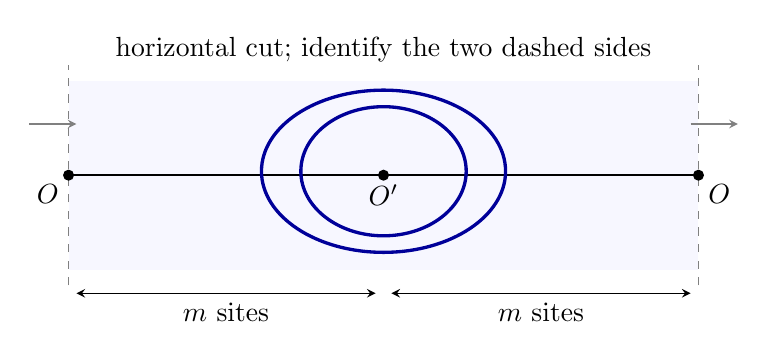
\begin{tikzpicture}[x=1cm,y=1cm,>=stealth]
 \fill[blue!3] (0,-1.2) rectangle (8,1.2);
 \draw[dashed,gray] (0,-1.4)--(0,1.4);
 \draw[dashed,gray] (8,-1.4)--(8,1.4);
 \draw[thick] (0,0)--(8,0);
 \fill (0,0) circle(2pt) node[below left] {$O$};
 \fill (4,0) circle(2pt) node[below] {$O'$};
 \fill (8,0) circle(2pt) node[below right] {$O$};
 \draw[<->] (.1,-1.5)--(3.9,-1.5) node[midway,below] {$m$ sites};
 \draw[<->] (4.1,-1.5)--(7.9,-1.5) node[midway,below] {$m$ sites};
 \draw[very thick,blue!60!black] (4,.05) ellipse (1.05 and .82);
 \draw[very thick,blue!60!black] (4,.05) ellipse (1.55 and 1.03);
 \draw[->,gray] (-.5,.65)--(.1,.65);
 \draw[->,gray] (7.9,.65)--(8.5,.65);
 \node at (4,1.6) {horizontal cut; identify the two dashed sides};
\end{tikzpicture}

\caption{The balanced cylinder, shown cut open along its seam. The two
marks split a period into equal site lists. The drawn nested cycles
separate the marks; the definition also permits noncontractible
separating cycles. The drawing is schematic rather than a lattice
embedding.}\label{j:fig-cylinder}
\end{figure}

For a regular tessellation hexagon $D_R$ of integer side length $R$, let
$\mathcal Z(R)$ be the partition of disjoint polygons contained in $D_R$
and surrounding its central face, each weighted by $2x^{|\lambda|}$;
the empty collection contributes one. Let $\mathcal C_R$ consist of
the ordered first-exit chords of $D_R$ whose diameter is at least $R/10$.
Both boundary ports are free: the sum includes every starting port and
every possible first-exit port, retaining the direction from start to
exit. Define the finite partition and probability law by
\[
 Z_R^{\rm chord}=\sum_{\gamma\in\mathcal C_R}x^{N(\gamma)},\qquad
 \mathbb P_R^{\rm chord}(\gamma)
   =\frac{x^{N(\gamma)}}{Z_R^{\rm chord}}\quad(\gamma\in\mathcal C_R).
\]

For a positive quantity $F(R)$, the notation $F(R)=R^{a+o(1)}$ means
$\log F(R)/\log R\to a$. An upper bound $F(R)\le R^{a+o(1)}$ means
that for every $\epsilon>0$ it is at most $C_\epsilon R^{a+\epsilon}$.
Uniform occurrences of this notation have constants and thresholds
independent of the indicated geometric data.

\begin{theorem}[Cylinder pressure and planar nesting]\label{j:cylinder}
As $m\to\infty$ through even integers,
\[
 G_m(2)=m^{1/6+o(1)},\qquad
 -\left.\frac{d^2}{dg^2}\log G_m(g)\right|_{g=0}=O(\log m).
\]
The derivative is the total basic weight of ordered incompatible pairs
of separating cycles, including a cycle paired with itself. Locally
uniformly for complex $\Theta$ with $|\Re\Theta|<\pi$,
\[
 |G_m(2\cos\Theta)|
 \le m^{\Re(1/6-2\Theta^2/(3\pi^2))+o(1)}.
\]
The planar partition satisfies $\mathcal Z(R)=R^{1/12+o(1)}$ as $R$ tends
to infinity through integers.
\end{theorem}

\begin{theorem}[Finite chords and marked polygons]\label{j:hexagon}
For the chord law just defined,
\[
 Z_R^{\rm chord}=R^{3/4+o(1)},\qquad
 \mathbb E_R^{\rm chord}N=R^{4/3+o(1)}.
\]
Uniformly for honeycomb vertices $v$ at distance at most $R/10$ from the
hexagon center,
\[
 \mathbb P_R^{\rm chord}(v\in\gamma)=R^{-2/3+o(1)}.
\]
Furthermore, for planar polygons modulo lattice translations,
\begin{equation}\label{j:polygon-square}
 \sum_{\operatorname{diam}\lambda\le H}
      x^{|\lambda|}|\lambda|^2\le H^{2/3+o(1)}.
\end{equation}
\end{theorem}

The chord conclusions describe this finite law, which is normalized
over all lengths allowed by the domain and the diameter cutoff. The
visit estimate concerns the stated bulk vertices. The final inequality
sums closed polygons modulo translations. Its proof uses the
positive mass of single polygons passing through two specified bonds
on a tilted cylinder. Theorem~\ref{j:unequal}, stated at the start of
Section~\ref{c7:marked}, gives the precise restrictions on the two site
lists and the uniform estimate used for this purpose.

\subsection{Earlier work}

Nienhuis's analysis of the dilute $O(n)$ model predicted the
two-dimensional self-avoiding-walk exponents \cite{Nienhuis1982}.
The conventional spatial prediction is $\nu=3/4$: the mean-square
displacement of a uniform length-$n$ walk is expected to be
$n^{2\nu+o(1)}$ \cite[Equation~(8)]{DuminilCopinSmirnov2012}.
The reciprocal $1/\nu=4/3$ motivates the length exponent in our finite
chord law, whose normalization and boundary conditions are specified above.
Duminil-Copin and Smirnov proved the exact honeycomb connective constant
by a parafermionic local cancellation and a boundary-flux argument
\cite{DuminilCopinSmirnov2012}. Their theorem determines the critical
activity used here. The local cancellation also gives a positive bound
on a convex boundary partition; the chord law requires quantitative
control of the part carried by macroscopic exits.
The vanishing of critical bridge mass was proved by Beaton,
Bousquet-M\'elou, de Gier, Duminil-Copin and Guttmann
\cite{BeatonEtAl2014}. For honeycomb bridges, Glazman and Manolescu
subsequently obtained a logarithmic subsequence bound. For their specified
columnwise rhombic half-plane tilings they also proved invariance of boundary
two-point functions \cite[Theorem~1 and Proposition~1.1]{GlazmanManolescu2017}.
Krachun and Panagiotis obtained a polynomial upper bound on the critical
bridge partition and used it to prove quantitative sub-ballisticity for
uniform length-$n$ honeycomb walks \cite{KrachunPanagiotis2026}.
These results concern distinct normalizations and precision levels;
our boundary proof establishes the radius-arch exponent with arbitrary
exponent slack.

The extension to rhombic weights connects this cancellation to
Yang--Baxter methods \cite{GlazmanManolescu2017}. Our local-weight and
fusion calculations keep the physical normalization explicit.

Grimm and Pearce developed a two-colour braid--monoid formulation of
dilute loop models and its Yang--Baxterization
\cite[Sections~4.2 and~4.6]{GrimmPearce1993}. The trigonometric weights
underlying the rhombic model trace back to Nienhuis
\cite{Nienhuis1990CriticalMulticritical,GlazmanManolescu2017}.
Finite-size corrections to periodic dilute-loop transfer-matrix spectra
have integrable-model predecessors \cite{ZhouBatchelor1997}.
For an open-strip dilute $O(1)$ model, Feh\'er and Nienhuis derive fusion
and current recursions \cite{FeherNienhuis2018}. Their current interpolation
in Section~6 uses rapidity-symmetry hypotheses stated in Section~5;
Appendix~E supplies a boundary fusion construction and explains why that
construction does not establish the current symmetries. The finite observable
here is different, and the symmetry within each of its two site groups is
proved directly. These earlier spectral and current formulas do not by
themselves identify its marked vacuum pairing or physical normalization.

The fermionic contractions and bosonic oscillator conversion belong to
the classical Wick and boson--fermion methods
\cite{Wick1950,Frenkel1981,FrenkelJingWang2000}; we compute their
twist, charge conventions and analytic limits in the normalization
needed here.

\subsection{Proof strategy}

The cylinder calculation begins by orienting occupied edges, with the
three states empty, forward and backward. Phases attached to turns,
seam crossings, and crossings of $A$ make the two orientations of a
loop cancel unless it separates the marks; a separating loop contributes
$g$. Long stacks with empty rims converge to vectors indexed by spin
configurations on the cut, whose pairing with the cut insertion gives
the partition. Finiteness of the total half-plane arch weight, proved in
Section~\ref{j:local}, justifies their limits. Section~\ref{c7:finite}
then uses local exchange and fusion, a spectral projector, and
polynomial interpolation to obtain an exact finite sum over three-valued
site spins. It temporarily allows arbitrary consecutive lists $A,B$
and nonzero complex spectral variables at their sites. The balanced
honeycomb case is recovered by choosing equal list sizes and setting
all site spectral variables to $1$.

Individual terms in this spin sum have poles when these variables
coincide, although the combined expression is regular.
Sections~\ref{c7:contour} and \ref{c7:boson} replace the sum by contour
residues, separate the coincident sites, and express the contractions
as an angular fermion trace. Evaluating that trace in oscillator
coordinates gives a gas on a horizontal circle of auxiliary length
$T$. Its particles have two species, corresponding to $A$ and $B$,
and carry integer charges. The gas records a running total charge, an
integer that changes by minus each particle's total charge as particles are
crossed. The resulting weights are signed or complex.
For the balanced cylinder, the limit $T\to\infty$ is taken at each fixed
site count; the estimates in the site count come afterward.

Section~\ref{c7:stability} controls the absolute gas weights by a
quadratic cost in the number of particles in each box and in this
running total charge at box boundaries. Section~\ref{c7:compact} uses
this estimate to form a
compact block propagator, with a contracting auxiliary coordinate
carrying the interaction with earlier blocks exactly. The site factors
suppress certain particle types on a central interval of length
proportional to $\log m$. The limiting operator there omits those types;
the exterior operator allows all types. Their propagation rates therefore
produce a power of $m$.

The exterior operator still has signed weights, and its eigenvalues of
maximal modulus may have Jordan blocks. At fixed $m$, the finite identity
supplies a limit in which the perturbed trace minus the normalized
physical value times the unperturbed trace tends to zero.
After normalization by the spectral radius,
Lemma~\ref{j:trace-extraction} expands the $n$th power of the exterior operator into
factors $\zeta^n$ with $|\zeta|=1$, multiplied by polynomials in $n$,
and compares the polynomial coefficients in the trace identity. This
retains all Jordan terms and bounds the
physical value without dividing by a trace that may cancel.
The Pfaffian scalar computed in Section~\ref{c7:pfaffian}, the exact
normalization $G_m(0)=1$, and positivity of the coefficients of $G_m$
then give the cylinder exponent and the incompatible-pair bound.

The chord mean also requires the size of its own finite partition
$Z_R^{\rm chord}$. The local boundary balance controls the total exit
weight from a port; the chord partition requires the part carried by
macroscopic exits. Write $W_R$ for the total critical weight of
first-exit same-boundary arches in a half-plane bounded by a horizontal
tessellation line that start at a fixed port and reach distance at least
$R$. Section~\ref{c7:boundary}
determines $W_R$ by an argument depending on the local transfer
identities and independent of the compact propagator. The added-row
expansion identifies the derivative of a one-row auxiliary cylinder increment
with its circumference $M$ times the deficit left in the boundary
balance by half-plane arches that embed in that cylinder. Fusion gives
functional relations for the increment, which determine the derivative
through a positive density on ordered points $0<k_1<\cdots<k_M$ whose
additional factor is an average over unitary conjugates. Comparison
with ensembles whose orthogonal polynomials can be evaluated gives the
derivative exponent $3/4$. The resulting deficit recovers the full
mass in the boundary balance and gives an upper bound for the endpoint tail
and a lower bound for the radius tail. A wedge comparison supplies the
matching radius upper bound, hence $W_R=R^{-1/4+o(1)}$. A boundary
comparison transfers this estimate to macroscopic hexagon exits;
summing over the free starting ports gives
$Z_R^{\rm chord}=R^{3/4+o(1)}$.

Proposition~\ref{j:visit} applies the boundary balance after removing
the triangle centered at a honeycomb vertex $v$ not adjacent to a
boundary port. It compares the raw weight of chords visiting $v$ with
the sum of the nesting partitions around its three incident
faces. For vertices within $R/10$ of the hexagon center, every such
chord meets the diameter cutoff when $R$ is sufficiently large.
Summing over vertices bounds the mean below by a constant times
$R^2\mathcal Z(\lfloor R/2\rfloor)/Z_R^{\rm chord}$ and above by a
constant times $R^2\mathcal Z(3R)/Z_R^{\rm chord}+R$; the additive term
accounts for vertices adjacent to boundary ports.
Section~\ref{c7:localization} uses the $O(\log m)$ incompatible-pair
bound to show that the sum of $x^{|\lambda|}$ over all noncontractible
separating cycles and all contractible cycles whose disk lifts are not
confined within a fixed multiple of $m$ around their enclosed mark is
$O(\sqrt{\log m})$. Their contribution costs a subpower factor.
The remaining cycles lift near one of the marks, giving upper and
lower comparisons of $G_m(2)$ with products of planar nesting
partitions at comparable radii. This gives
the exponent $1/12$; the visit comparison and chord normalization then
give the mean and bulk-visit exponents.

The length-square mass is handled through the positive sum of
$x^{|\lambda|}$ over single polygons using two specified bonds. After
a lattice rotation or reflection, the marked estimate in
Theorem~\ref{j:unequal} applies to cylinders whose cuts use horizontal
tessellation steps and steps tilted by $\pi/3$. Both marked bonds cross
horizontal steps, and the proportions of the two directions in each
unmarked list satisfy the restrictions in that theorem.
Sections~\ref{c7:marked}--\ref{c7:shifted} derive the matrix and
horizontal representations of this two-bond sum, including their
scalar normalization and uniform suppression for those lists. If
their sizes are $m$ and $n$, the two suppression
intervals have lengths proportional to $\log m$ and $\log n$. On the
parts covered by only the longer interval, the mixed propagator allows
all types in one species and only the unsuppressed types in the other.
Section~\ref{c7:mixed} bounds this propagator by a separate calculation
with one species. Monotonicity of the running total charge
controls the central region where both suppressions act. The final
counting argument sums the marked estimate over selected bond pairs whose
displacements fit these cuts and
separately bounds polygons for which too few such pairs are available.
This proves
\eqref{j:polygon-square}.

\section{Boundary balance and local transfer identities}\label{j:local}

We first prove the local identities used by both cylinder observables. The boundary balance also shows that the total half-plane arch weight is finite; this finiteness justifies the vacuum limits in Section~\ref{c7:finite}. The sharper arch exponent is proved in Section~\ref{c7:boundary}.

We keep the lattice, ports and first-exit convention of the introduction.
In particular a walk traversing $N$ triangle centers has weight $x^N$,
where $x=(2+\sqrt2)^{-1/2}$. The local turning balance is the
Duminil-Copin--Smirnov parafermionic cancellation. The extension to
rhombic tiles uses the Yang--Baxter weights discussed by Glazman and
Manolescu \cite{DuminilCopinSmirnov2012,GlazmanManolescu2017}.

The boundary estimate ultimately obtained in Section~\ref{c7:boundary} is: in the half-plane bounded by a horizontal tessellation line, the total weight $W_R$ of boundary-to-boundary walks from a fixed port reaching Euclidean distance $R$ or more from that port satisfies
\[
W_R=R^{-1/4+o(1)}.
\]

\label{j:convex-balance}
Write $s=3/8$, $\alpha=\pi/8$, so $2x\cos(s\pi/3)=1$. For any finite convex tessellation polygon $D$ and starting port $a$, the sum over all SAWs to ports, with the extra factor $e^{isT}$ for total turning $T$, is 1. In fact, extend the nonbacktracking walk from vertex to vertex, with factors $xe^{\pm is\pi/3}$ summing to 1, and stop before traversing an already visited vertex. Ends of this tree due to first collision cancel: after a common incoming stem there are two ways around the newly formed simple loop, and the stem approaches the loop from outside. The turn at closure would be $\pm\pi/3$ (unused third branch outside means a convex corner); thus other loop vertices contribute $\pm5\pi/3$ and the turn from the stem onto the loop $\mp\pi/3$. The extra factor therefore sums to $2\cos(4\pi s/3)=0$. For the walks to ports $b$, $T=\Delta-\pi$ where $\Delta$ is the counterclockwise boundary tangent turn accumulated from $a$ to $b$ (close the walk along the boundary from $b$ to $a$, giving positive orientation and two extra quarter turns). In particular $\cos(sT)\ge\sin\alpha>0$. This turning calculation is the local parafermionic balance in path form. \cite{DuminilCopinSmirnov2012}

Let $H(d)$ denote the half-plane arch weight from a port to a port $d$ steps to the right. Reflection gives the same weight to the left; by convex exhaustions $2\sin\alpha\sum_{d>0}H(d)\le1$.

\subsection{An auxiliary cylinder and spectral equation}
Take a cylinder obtained by identifying modulo $M$ steps horizontally, tiled by rows of $M$ rhombi each, with basis $1,e^{i\theta}$ and potentially a different $\theta$ per row. Connections inside a tile link pairs of bond midpoints on distinct sides, using each at most once, noncrossingly. The empty weight is 1, a straight connection between opposite sides weighs $v$, the single turns of absolute angles $\theta,\pi-\theta$ weigh $u,d$ respectively (port directions normal to sides); and two simultaneous turns weigh $a$ for the pairing left--down and up--right, or $b$ for left--up and right--down. With $\phi=3\theta/8$, $s_k=\sin(\phi+k\alpha)$, $h=\sin(2\alpha)$, use the trigonometric SAW weights
\[
(u,d,v,a,b)=\frac{(h s_5,h s_0,s_0s_5,s_5s_6,-s_0s_7)}{s_2s_3}.
\]
At $\phi=\alpha$ these are $(x,x^2,x^2,x^2,0)$, exactly the original lattice rules (split each tile into the two equilateral triangles). The relation between rhombic geometry, parafermionic cancellation and
integrable loop weights was developed by Ikhlef and Cardy
\cite{IkhlefCardy2009}. Glazman's corrected general loop-weight formulas
\cite[Section~5]{Glazman2015} give a useful comparison; the five weights
and their critical specialization here are checked directly below.
See also the boundary two-point results in \cite{GlazmanManolescu2017}.

For a finite stack, close both rims (require unused ports). The partition $Z$ of \textbf{one noncontractible polygon only} (unoriented, unrooted) is the linear coefficient in fugacity $n$ of the full loop sum giving weight zero to contractible loops and weight $n$ per noncontractible loop. For real angles $0<\theta<\pi$, orient loops with factor $\exp(-iT/4)$ and twist $p$ to the power signed number of seam crossings (east positive); summing orientations effects precisely these loop weights for $n=p+p^{-1}$. Indeed disjoint arcs can be drawn in tiles with the indicated tangent turns; an embedded loop in the flat cylinder is either contractible with turn $\pm2\pi$ or has winding $\pm1$ and turn zero. For instance the latter follows by mapping conformally by an exponential to a round annulus and using the plane turning formula there. These identities then extend algebraically. 

The oriented matrix, with spins $0,\pm1$ on horizontal-flow and descending-flow bonds (respectively across the sides parallel to $e^{i\theta}$ and to $1$), has row indices (left, up), column indices (right, down), positive signs meaning left to right or up to down. Remove the phase $e^{i\theta(\text{left}-\text{right})/4}$ (telescoping). The resulting $R(\phi)$ conserves the sum, with blocks, $\lambda=e^{-2i\alpha}$:
\[
\begin{array}{c|c}
(s',s')\quad(s'=\pm1)& a\\
(s',0),(0,s')&\begin{pmatrix}v&u\\u&v\end{pmatrix}\\
(1,-1),(0,0),(-1,1)&
\begin{pmatrix}
 b&d\lambda& b\lambda^2+a\\
 d\lambda^{-1}&1&d\lambda\\
 b\lambda^{-2}+a&d\lambda^{-1}&b
\end{pmatrix}
\end{array}
\]
(the turns connecting left to down have magnitude $\theta$, those connecting left to up have magnitude $\pi-\theta$).

\subsection{Local exchange and fusion}

The matrix identities below have two uses. Exchange lets us interchange
two rows of local matrices. Fusion identifies the action on a smaller auxiliary
space; at a matching site the action on the quotient vanishes. We treat
these as meromorphic identities, including at the rank-deficient fusion
matrices.

Let $V=\mathbb C^3$ with basis $|0\rangle,|+\rangle,|-\rangle$, and use
subscripts to indicate an ordered pair of tensor factors. On a copy
$V_i$, let $s_i|k\rangle_i=k|k\rangle_i$. Write $P_{ij}$ for the
interchange of factors $i,j$, and put
\[
\Delta_R(\psi)=\sin(\psi+2\alpha)\sin(\psi+3\alpha).
\]
\begin{lemma}[Local exchange and fusion]\label{j:local-exchange-fusion}
The entries of $R(\psi)$ are meromorphic, with possible poles at
$\Delta_R(\psi)=0$. The following are identities of meromorphic matrix
functions:
\[
\begin{split}
R_{12}(t)R_{13}(t+\phi)R_{23}(\phi)
 &=R_{23}(\phi)R_{13}(t+\phi)R_{12}(t),\\
R_{12}(\phi)R_{21}(-\phi)&=I.
\end{split}
\]
In particular the second equality is a pointwise inverse identity
where both factors are regular, and $R_{12}(0)=P_{12}$.

For $\delta=2,3$, let $E_2=V$, $E_3=\mathbb C$, and define injective
maps $J_\delta:E_\delta\to V\otimes V$ by
\[
\begin{aligned}
J_2|0\rangle&=|00\rangle+x\sum_{k=\pm1}\lambda^k|k,-k\rangle,
&J_2|k\rangle&=x(|k,0\rangle+|0,k\rangle)\quad(k=\pm1),\\
J_3(1)&=\sum_{k=0,\pm1}\lambda^k|k,-k\rangle.
\end{aligned}
\]
On $E_2$ let $s_{\rm f}|k\rangle=k|k\rangle$, and on $E_3$ let
$s_{\rm f}=0$.
Then $R_{12}(\delta\alpha)=J_\delta J_\delta^*$ and, writing $J=J_\delta$,
\[
R_{23}(\phi)R_{13}(\phi+\delta\alpha)(J\otimes I)
 =(J\otimes I)R_{\rm f}(\phi),\qquad
R_{\rm f}(\phi)=
\begin{cases}
R(\phi+\alpha),&\delta=2,\\
I,&\delta=3.
\end{cases}
\]
The intertwining equality is again meromorphic in $\phi$.
\end{lemma}
\begin{proof}
At $0,2\alpha,3\alpha$ the five weights are, respectively,
$(1,0,0,1,0)$, $(x^2,x,x^2,0,x^2)$ and $(0,1,0,0,1)$.
The blocks give $R_{12}(0)=P_{12}$ and the two factorizations directly. For example,
the charge-zero column of $J_2$ is
$(x\lambda,1,x\lambda^{-1})^T$, and the charge-$\pm1$ columns are
$x(1,1)^T$. These are embeddings rather than isometries:
$J_2^*J_2=\operatorname{diag}(3-\sqrt2,2-\sqrt2,2-\sqrt2)$ in the
displayed basis, and $J_3^*J_3=3$.

For regular $\phi$ and $-\phi$, unitarity follows by block multiplication,
using $\lambda^4=-1$. With primes denoting $-\phi$, the required scalar
relations are
\[
aa'=1,\quad ab'+ba'+dd'=0,\quad ad'+d=a'd+d'=0,
 \quad vv'+uu'=1,\quad vu'+uv'=0
\]
by $s'_j=s_{8-j}$ and the sine products above. For instance the first
diagonal entry of the charge-zero product is
$aa'+\lambda^2(ab'+ba'+dd')$, and its adjacent entry is
$\lambda(ad'+d)$. Since these are rational trigonometric identities,
unitarity follows meromorphically as stated.

Writing $B(i,l;j,k;\phi)$ for entries of $R$, the same blocks give
\[
B(i,l;r,k;\phi+3\alpha)=\lambda^{k-l}B(l,-r;k,-i;-\phi)
\]
(weights swap $u,d$ and $a,b$, keeping $v$). Thus for the single column intertwining, the coefficient is
\[
\sum_r B(j,m;-r,l;\phi) B(i,l;r,k;\phi+3\alpha)\lambda^r
=\lambda^i\delta_{j,-i}\delta_{m,k},\qquad l=r+k-i,
\]
with out-of-range entries zero.

For the other intertwining, denote the five weights at $\phi+2\alpha$ by $U,D,V,A,B_0$, at $\phi+\alpha$ by $w,X,g,e,f$. To detail the block multiplication, the components with inputs fused spin $r$ and site spin $k$, outputs $i,j,m$ ($i+j+m=r+k$) are
\[
\sum_t J_{t,r-t;r}\, R(\phi+2\alpha)_{i,t+k-i;t,k}\,R(\phi)_{j,m;r-t,t+k-i}
 = J_{i,j;i+j} R(\phi+\alpha)_{i+j,m;r,k}.
\]
It suffices (opposite spins conjugate the phases) to check the following scalar identities for each group after substitution and $\lambda^2+\lambda^{-2}=0$:
{\small
\[
\begin{array}{c|l}
(r,k) &\\ \hline
(1,1) & Va=Av+Uu=e,\quad Au+Uv=0\\
(1,0)& Da=w,\quad x(Uv+u)=w,\quad Uu+v=Dd+V=g,\quad Db+Vd=0\\
(0,1)& B_0 a=g,\quad x D u+Vv=g,\quad x Dv+Vu=xw,\quad x(Aa+B_0 b)+Ud=0,\quad xB_0 d+U=xw\\
(1,-1)& B_0 v=Dd+V b=f,\quad B_0 u=x(D+Vd)=X,\quad Va=Av+Uu=e,\quad Au+Uv=0\\
(0,0)& x Ua+d=x X,\quad D u+x Vv=x,\quad Dv+x Vu=x X
\end{array}
\]
}
For clarity $U,D,V,A,B_0$ have numerators $(h s_7,h s_2,s_2 s_7,-s_0s_7,s_2s_1)$ over $s_4s_5$, and $w,X,g,e,f$ numerators $(h s_6,h s_1,s_1s_6,s_6s_7,s_1s_0)$ over $s_3s_4$. Direct common factors cancel; the remaining identities reduce to
\[
\begin{gathered}
 s_2s_6=h^2-s_0^2=x(s_0s_7+s_4s_5),
 \quad s_1s_5=h^2-s_7^2=x(s_0s_7+s_2s_3),\\
 s_1-s_7=s_0/x,\quad s_6-s_0=s_7/x,\\
 s_0s_1+s_4s_5=s_2s_3+s_6s_7=s_1s_2+s_5s_6=h^2/x,\\
 s_1s_6-s_0s_7=h^2 x,\quad s_3s_4-s_0s_7=h^2/x,\quad
 x(s_5s_6-s_0s_1)=s_3s_7,\quad x(s_1s_2-s_6s_7)=s_0s_4,
\end{gathered}
\]
all by product-to-sum.

For regular real parameters the matrices are Hermitian. The intertwining
and its adjoint therefore give the three-space exchange at
$t=2\alpha,3\alpha$; the swap gives it at $t=0$. Interchange spaces
2 and 3 in these equalities and apply unitarity at a generic $\phi$.
This gives exchange also at $t+\phi=0,2\alpha,3\alpha$.

It remains to see why these special values determine the identity.
Every entry of $\Delta_R(\psi)R(\psi)$ has Fourier exponents between
$-2$ and $2$. Moreover, if $Z|k\rangle=(-1)^{k^2}|k\rangle$, then
$R(\psi+\pi)=Z_1R(\psi)Z_1$: only the single-turn weights change
sign. After multiplying the exchange difference by
$\Delta_R(t)\Delta_R(t+\phi)\Delta_R(\phi)$, each entry consequently
has exponents between $-4$ and $4$ in $e^{it}$, all of one parity.
After a monomial factor it is a polynomial in $e^{2it}$ of degree at
most $4$. The six values
$0,2\alpha,3\alpha,-\phi,2\alpha-\phi,3\alpha-\phi$ are distinct
modulo $\pi$ for generic real $\phi$, so the polynomial vanishes.
Continuation in the two parameters proves the meromorphic identity.
\end{proof}

\begin{lemma}[Restriction and quotient at fusion]\label{j:local-restriction}
Fix $\delta\in\{2,3\}$, put $W_\delta=\operatorname{im}J_\delta
\subset V_1\otimes V_2$, and for another factor $V_k$ set
\[
F_{\delta,k}(\psi)=R_{2k}(\psi)R_{1k}(\psi+\delta\alpha).
\]
At regular parameters the subspace $W_\delta\otimes V_k$ is invariant,
and transporting the restriction through $J_\delta\otimes I$ gives $R_{\rm f}(\psi)$ from
Lemma~\ref{j:local-exchange-fusion}. At $\psi=0$ the full image of
$F_{\delta,k}(0)$ lies in this subspace. Hence the induced operator on
$\bigl((V_1\otimes V_2)/W_\delta\bigr)\otimes V_k$ is zero there and, near
$z=e^{2i\psi}=1$, is holomorphic and divisible by $z-1$.

The twist restricts by
$p^{s_1+s_2}J_2=J_2p^{s_{\rm f}}$ and
$p^{s_1+s_2}J_3=J_3$ for every $p\ne0$.
There is also the meromorphic site intertwining
\begin{equation}\label{j:site-fusion}
R_{a1}(\psi)R_{a2}(\psi+\delta\alpha)(I_a\otimes J_\delta)
 =(I_a\otimes J_\delta)
\begin{cases}
R_{a{\rm f}}(\psi+\alpha),&\delta=2,\\
I_a,&\delta=3.
\end{cases}
\end{equation}
\end{lemma}
\begin{proof}
Invariance and the restricted action are the preceding intertwining.
Write $J_{\delta,1k}$ for the embedding on factors 1 and $k$, with
the other factor unchanged.
At the matching point the factorization supplies the stronger inclusion
\[
F_{\delta,k}(0)=P_{2k}R_{1k}(\delta\alpha)
 =P_{2k}J_{\delta,1k}J_{\delta,1k}^*,
\qquad
\operatorname{im}F_{\delta,k}(0)\subseteq W_\delta\otimes V_k.
\]
Indeed $P_{2k}$ carries the image of $J_{\delta,1k}$ to that of
$J_{\delta,12}$. The quotient operator is holomorphic near zero because
the local parameters $0,\delta\alpha$ are regular. Its vanishing gives
the claimed factor in the local coordinate $z-1$. The twist formulas
follow because every term of $J_2|s_{\rm f}\rangle$ has total spin
$s_{\rm f}$ and every term of $J_3$ has total spin zero.

For real regular parameters the blocks give
$\overline{R_{ij}}=R_{ji}$ and $P_{12}\overline{J_\delta}=J_\delta$.
Conjugating the row intertwining and exchanging spaces 1 and 2 gives
\eqref{j:site-fusion}; continuation gives its meromorphic form.
\end{proof}


\subsection{A Fourier identity for the scalar kernels}

The finite vacuum normalization and the later boundary moment problem
use the same elementary transform. Recording it here makes both
calculations independent of their order.

\begin{lemma}\label{j:fourier-kernel}
For $0<\beta<\pi$ and $|\Im y|<\pi-\beta$,
\[
 \int_{\mathbb R}e^{iky}\frac{\sinh(\beta k)}{\sinh(\pi k)}\,dk
 =\frac{\sin\beta}{\cosh y+\cos\beta}.
\]
The integral and its parameter derivatives converge locally uniformly
on the indicated strip.
\end{lemma}
\begin{proof}
For real $y>0$, close the contour by rectangles in the upper half-plane
with upper edges at half-integer heights. The ratio of hyperbolic sines
decays exponentially on the vertical edges as their real coordinates
tend to infinity; the factor $e^{iky}$ controls the upper edge as its
height tends to infinity. The residues at $k=in$, $n\ge1$, give
\[
 2\sum_{n\ge1}(-1)^{n+1}\sin(n\beta)e^{-ny}
 =\frac{\sin\beta}{\cosh y+\cos\beta}.
\]
The geometric series proves the last equality. Evenness extends it to
negative real $y$, and dominated convergence covers $y=0$.
Exponential decay in $|k|$ proves local uniform convergence and
parameter differentiation on smaller strips. Analytic continuation
then gives the asserted domain.
\end{proof}

\section{The two-puncture observable and its finite spin formula}\label{c7:finite}

We construct the finite cylinder observable that determines the nesting
partition. Orienting the loops expresses it as a pairing of two vacuum
vectors. We then identify the scalar factor that clears the denominators
of these particular vectors and use their polynomial degrees and fusion
values to determine the spin formula. The same vector statement will
also supply the regularity needed for the two marked bonds.

Keep the honeycomb cylinder of circumference $M$, first with finite height on either side of a cut along a horizontal tessellation line. Mark two face centers (tessellation vertices) $O,O'$ on the cut, the first at the seam, dividing the sites into consecutive groups $A,B$ in eastward order starting at $O$. Close both rims. Use any collection of disjoint simple cycles, \emph{each separating} $O,O'$, with weight $x^{|\gamma|}g$ per cycle, $x$ the critical weight above. Write $G_{A,B}(g)$ for this partition including the empty term, with the height sent to infinity. We use $g=h+h^{-1}$ (in this part $h$ denotes a twist parameter, not the sine constant in the weights). The degree in $g$ is bounded by $M$ since the cycles must intersect the arc of the cut from $O$ to $O'$.

Here and below matrices of oriented weights and their spectral parameter $\phi$ refer to $R(\phi)$ above, $\lambda=e^{-2i\alpha}$ and $\alpha=\pi/8$. The rhombic Yang--Baxter setting and periodic dilute-loop spectra have the precedents \cite{GlazmanManolescu2017,ZhouBatchelor1997}. The current calculation of \cite[Section~6]{FeherNienhuis2018} is a related recursion under a rapidity-symmetry hypothesis; our finite observable and its symmetry are derived below.

\subsection{The oriented observable and its vacuum limits}

Put $q=e^{2i\alpha}=\lambda^{-1}$, introduce site variables $x_j=e^{2i\phi_j}$ (not vertex fugacities), and, with $w=e^{2i\xi}$, set
\[
T_p(w)=\mathrm{Tr}_a\, p^{s_a} R_{a1}(\xi-\phi_1)R_{a2}(\xi-\phi_2)\cdots R_{aM}(\xi-\phi_M),
 \qquad p\in\{i,-i\}.
\]
Here $s_j$ is the diagonal spin, index $a$ the auxiliary space. We work
on the total site charge zero subspace
\[
\mathcal H_M=\operatorname{Span}\{|\sigma\rangle:
\sigma\in\{-1,0,1\}^M,\ \sum_j\sigma_j=0\}
\]
and denote its empty vector by $|0\rangle$. Choices of square roots of
the variables are understood. For each fixed $p$, the rows commute by
Lemma~\ref{j:local-exchange-fusion}. The vacuum matrix element satisfies
\[
\langle0|T_{p_1}(w_1)\cdots T_{p_L}(w_L)|0\rangle=1
\]
for arbitrary words in the two twists, at regular parameters. Indeed the
oriented phases in the blocks can still be drawn on the reference tiling
with fixed angle $\pi/3$, keeping the angle-independent phases after
removing the telescoping factor and varying only the scalar weights of
the tile pictures. Each contractible loop has phase $\pm i$ before seam
signs, and each noncontractible one has turn zero and winding $\pm1$.
Seam factors for either orientation are those for uniform twist $i$,
times the same sign from the layers of twist $-i$. All loops therefore
cancel.

We will use this word identity in two ways. First, every linear
combination $A$ of operators $T_p(w)-I$, even with the two twists mixed,
has zero as an eigenvalue: $\langle0|A^k|0\rangle=0$ for $k\ge1$, and
the characteristic polynomial would contradict this if its constant
term were nonzero. Second, fix one twist $p$. Choose finitely many row
deviations spanning the linear span of all $T_p(w)-I$ in
$\operatorname{End}\mathcal H_M$ and simultaneously triangularize them. For every
choice of coefficients, one diagonal character of the corresponding
linear combination vanishes. A finite union of proper hyperplanes
cannot cover the coefficient space, so one character vanishes
identically. Thus this fixed-twist family has the simultaneous
eigencharacter $T_p(w)=1$.

For physical site variables all one, use twist $p=-i$ above the cut and $p=i$ below, with the insertion
\[
D_A=(ih)^{\sum_{j\in A}s_j}.
\]
To check the weight, orient a contractible simple cycle counterclockwise or a noncontractible one eastward, and let $I_1,I_2$ indicate whether $O,O'$ belong to its left component (interior or upper, respectively). The signed cut crossings in $A$ (downward positive) give $I_2-I_1$. Signed seam crossings above and below $O$ (eastward positive) give $-I_1,I_1$ in the contractible case and $1-I_1,I_1$ otherwise. These numbers follow by moving along the corresponding transverse arcs from component to component. Including turn, seam and insertion, the phase is $(-i)(-1)^{I_1}(ih)^{I_2-I_1}$, with its inverse for reversed orientation. Thus it cancels unless the cycle separates the marks, and then sums to $g$.

The top and bottom vacuum vectors tend to finite limits
$L_-^{\rm phys},R_+^{\rm phys}$; the subscripts $+,-$ on vacuum vectors
stand for twists $i,-i$. Untouched closed loops separately cancel,
leaving disjoint arcs connecting ports on the cut in each half-cylinder.
Any lift of such an arc has port separation less than $M$: otherwise its
endpoints interlace those of a period translate, contradicting
noncrossing. Products of finitely many half-plane arch sums $H(d)$ from
Section~\ref{j:local} therefore dominate the absolute weights.

These physical vectors have the simultaneous eigencharacter $T=1$ for
their respective twists. For example, insert a regular row $T_i(w)$
just below the cut and commute it to the far closed rim. With the rim
ports empty that row uses no double turn, so its absolute weights are
bounded by the physical weights times a constant depending on $M,w$.
An arc affected by the row must reach the receding rim. Its total weight
tends to zero by the same arch summability. The inserted row thus leaves
the limit unchanged, and the top vector is treated in the same way.
Both vacuum components are 1. This proves the height limit and finite
coefficient sums (for example by taking $g>0$), with
\[
G_{A,B}=L_-^{\rm phys}D_A R_+^{\rm phys}.
\]

\subsection{Fusion and the algebraic vacuum projector}

Write $H_p=T_p-I$. We first record the behavior of a local matrix when
$z=w/x_j$ tends to zero or infinity. Directly from the sine weights,
\[
\begin{array}{c|c|c}
 & (a,b,v)&(u,d)\\ \hline
z\to0&(q^{-3},q^3,1)&O(z^{1/2})\\
z\to\infty&(q^3,q^{-3},1)&O(z^{-1/2}).
\end{array}
\]
The entries are holomorphic in $z^{1/2}$ at zero and in $z^{-1/2}$ at
infinity. On a state with auxiliary spin $r$ and site spin $s$, the
diagonal limit is $q^{3rs}$ at infinity and $q^{-3rs}$ at zero. The
only surviving off-diagonal entry at infinity changes the auxiliary
spin from $-1$ to $1$ and the site spin from $1$ to $-1$ (row minus
column); at zero this move is reversed. In particular every surviving
move at an inactive site preserves its vacancy parity.

Square-root factors occur only in the single turns, which change
auxiliary vacancy parity. Their number in an auxiliary trace is even,
so $H_p(w)$ is rational in $w$, with possible simple poles
$q^5x_j,q^6x_j$ at generic sites. The same observation for a site says
that changing a square-root sign conjugates $T_p$ by
$P_j=(-1)^{s_j^2}$. At either endpoint of the row parameter, a closed
auxiliary trace cannot use a strictly one-directional off-diagonal
move. On $\mathcal H_M$ the remaining diagonal trace is
$\sum_{r=-1}^1p^r q^{\pm3r\sum_j s_j}=1$. Thus
$T_p(0)=T_p(\infty)=I$. With $C_\ell(z,b)=z/(z-q^\ell b)$ we obtain
\[
H_p(w)=\sum_{j=1}^M\sum_{t=0}^1 C_{5+t}(w,x_j) U_{jt},
\]
where the coefficient operators commute. The basis functions vanish at
zero and have distinct poles; the condition at infinity additionally
gives $\sum_{j,t}U_{jt}=0$.

The two embeddings and row fusion above give at any site $x_j$, generically,
\[
T_p(x_j)T_p(q^2x_j)=T_p(qx_j),\qquad T_p(x_j)T_p(q^3x_j)=I.
\]
Indeed the combined auxiliary monodromy has local factors
$R_{2k}(\phi)R_{1k}(\phi+\delta\alpha)$, with the lower parameter on
the left. Lemma~\ref{j:local-restriction} identifies their restriction
to $\operatorname{im}J_\delta$ and shows that the quotient factor at
site $j$ is zero: its full image is already in
$\operatorname{im}J_\delta\otimes V_j$. The quotient monodromy therefore
has zero trace. On the restriction the twist is the fused twist, or the
identity for $\delta=3$, giving the two formulas. This is a trace of
the restriction transported through $J_\delta$, so no isometry factor
enters. Square roots can be chosen consistently; shifting a whole row
parameter by $\pi$ leaves $T_p$ unchanged.

Set $T_j=T_p(x_j)$. Expanding the fusion formulas in the commuting
coefficients $U_{kt}$ gives a homogeneous system $\mathcal L(T)U=0$.
Its two rows for site $j$, with column site $k$, type $t$, and
$C_\ell=C_\ell(x_j,x_k)$, are
\[
\begin{split}
 C_{5+t}-C_{4+t}+T_j C_{3+t},\\
 C_{4+t}+T_j(C_{2+t}-C_{3+t}).
 \end{split}
\]
The second is the rank-one fusion equation minus the first. At $T=1$
these rows are $C_5+C_3-C_4$ on the same row and column list
$Y=(x_1,q x_1,\ldots,x_M,q x_M)$. Subtracting the constant $1/2$ gives
the skew kernel
\[
S(u,v)=\frac{(u-v)(2(u+v)^2-d(u,v))}{2(u+v)d(u,v)},\qquad d(u,v)=u^2+\sqrt2uv+v^2.
\]
The adjugate of an even skew matrix is skew. Adding a matrix with
constant entries therefore does not change its determinant, and
$\det\mathcal L(1)=(\operatorname{Pf}S(Y))^2$. Whenever this scalar
denominator is nonzero,
\[
\Pi_p=\frac{\det\mathcal L(T)}{\det\mathcal L(1)}
\]
is a projector onto the common fixed space. Indeed the determinant is
taken in the commutative algebra generated by the rows. The adjugate
identity for $\mathcal L(T)U=0$ shows that $\Pi_p$ annihilates every
$U_{jt}$, while on their joint kernel $T_j=1$ and $\Pi_p=1$. Hence its
image is exactly that kernel and it is idempotent. Evaluating its
polynomial numerator by the arbitrary-word vacuum identity also gives
\[
\langle0|\Pi_p|0\rangle
 =\langle0|\Pi_p\Pi_{p'}|0\rangle=1
\qquad(p,p'\in\{i,-i\}).
\]

\subsection{The scalar normalizers}

The denominator of the projector is governed by three scalar functions.
The factorization below separates the factor $N$, which will clear the
two selected vacuum vectors, from the additional factor $N_2^*$ present
for the full projector.

We use the Pfaffian of an even skew matrix: it is the signed matching
sum, equivalently the coefficient of the oriented volume form in the
normalized top power of its two-form. It transforms under simultaneous
row and column change by the determinant, and its square is the
determinant, as follows by reduction to two-dimensional skew blocks.
For the site list $X$, put
$\mathcal P(X)=\prod_{j<k}d(x_j,x_k)/(x_j-x_k)$ and define
\[
\begin{split}
 N(X)&=\mathcal P(X)\operatorname{Pf}_{j,k}\frac{x_j^2-x_k^2}{d(x_j,x_k)},\\
 N_2^*(X)&=\mathcal P(X)^2\det_{j,k}\frac{(2+\sqrt2)x_jx_k}{d(x_j,x_k)},\\
 \mathcal J(X)&=S(1,q)^{-M}\operatorname{Pf} S(Y)\prod_{j<k}P_*(x_j,x_k),\\
 P_*(u,v)&=\frac{(u+v)(u^2+v^2)d(u,v)^2}{(u-v)^2(u^2-\sqrt2uv+v^2)} .
 \end{split}
\]
When $M$ is odd, pad the Pfaffian defining $N$ by a last index whose
column entries above the diagonal are 1. All empty-list normalizations
are 1. Write $N_1=N$, $N_2=N_2^*$, $N_3=\mathcal J$, and set
\[
\ell_2(u,z)=z-q^5u,\qquad
\ell_3(u,z)=(z-q^5u)(z-q^6u).
\]
\begin{lemma}[Scalar normalizers]\label{j:scalar-normalizers}
For every list size $M$, the functions $N_l$ are symmetric homogeneous
polynomials of individual degree at most $l(M-1)$ for $M\ge1$, and
\[
\mathcal J=N N_2^*.
\]
For $l=1,2$ and $X=(u,Z)$ of size $M\ge1$, their deletion values are
\begin{equation}\label{j:normalizer-deletion}
N_l(0,Z)=\left(\prod_{z\in Z}z^l\right)N_l(Z),
\qquad [u^{l(M-1)}]N_l(u,Z)=N_l(Z).
\end{equation}
For $\delta=2,3$ all three satisfy
\begin{equation}\label{j:normalizer-fusion}
N_l(u,q^\delta u,Z)=N_l(u,q^\delta u)\ \prod_{z\in Z}\ell_\delta(u,z)^l\ N_l(X_{\rm red}),\qquad
 X_{\rm red}=\begin{cases}(qu,Z)&\delta=2,\\Z&\delta=3.\end{cases}
\end{equation}
At two sites,
\[
N(u,v)=u+v,\qquad
N_2^*(u,v)=u^2+2(1+\sqrt2)uv+v^2.
\]
Finally, $N$ and $N_2^*$ are nonzero at every homogeneous list
$(b,\ldots,b)$ with $b\ne0$.
\end{lemma}
\begin{proof}
We first remove the apparent poles. For $N$ and $N_2^*$ all $d$
denominators are cleared by $\mathcal P$ or $\mathcal P^2$. The
remaining numerator vanishes on equal sites by alternating rows, or by
alternating rows and columns, so it is divisible by the corresponding
Vandermonde factors.
The sign from a site interchange in the Pfaffian is canceled by that
of $\mathcal P$; the determinant has the corresponding row and column
signs. For $\mathcal J$, interchanging two paired blocks is an even
permutation. Thus all three functions are symmetric.

For $\mathcal J$, fix a pair of sites $u,v$ with $v=q^\delta u$ and
keep all other sites generic. In the skew kernel on the paired list
$Y$, repeated rows and columns give a zero of order at least two at
$\delta=0$ and at least one at $\delta=\pm1$. At $\delta=2$ the only singular
cross coupling is between $u,qv$, so there is at most a simple
Pfaffian pole. At $\delta=3$ there is at most a double pole, and the
reflected cases have the same bounds. At $\delta=4$ the $2\times2$
cross residue, up to a common scalar, has diagonal entries 1 and
off-diagonal entries $-1$. Its rank is one, so the potential double
pole cancels. The factors in
\[
P_*(u,v)=
\frac{(v-q^4u)(v-q^2u)(v-q^6u)
      (v-q^3u)^2(v-q^5u)^2}
     {(v-u)^2(v-qu)(v-q^7u)}
\]
clear these possible orders. These calculations are at generic points
of each possible divisor. Unique factorization then removes every
irreducible denominator; simultaneous intersections are included by
this polynomial conclusion.

Homogeneity follows from the displayed formulas, and the individual
degree bounds follow by taking a variable to infinity. For the paired rows of $\operatorname{Pf}S(Y)$
the cross rows have identical limits, so they decouple from the rest
of the Pfaffian. The deletion rules for $N,N_2^*$ follow in the same
way at zero and infinity. The extra determinant index decouples.
For the Pfaffian, place the varied variable first. Its row on the other
sites has constant limit $-1$ at zero and $1$ at infinity. Without
padding it becomes the padding row after reordering; with padding the
two constant rows pair off since their mutual coupling is 1. The signs
cancel those from $\mathcal P$, giving \eqref{j:normalizer-deletion}.

We next prove the reductions. For $\mathcal J$ the leading pole at
$\delta=3$ removes both pairs of site indices, while at $\delta=2$ the
pole between $u,q^3u$ leaves $qu,q^2u$, the pair for the reduced site.
The internal scalar is the two-site value. The remaining factors are
\[
P_*(u,z)P_*(q^3u,z)=\ell_3(u,z)^3,\qquad
\frac{P_*(u,z)P_*(q^2u,z)}{P_*(qu,z)}=\ell_2(u,z)^3.
\]
For $\delta=3$, the $d$ pole and $\mathcal P$ give the same reduction
for the first two polynomials.

For $N$ at $\delta=2$, first divide out
$\prod_{z\in Z}(z-q^5u)$. At each $z=q^5u$ the prefactor has two
zeros, whereas the Pfaffian has at most one pole because the two
singular entries share the index $z$. After division, compare the two
sides as polynomials of degree at most $M-2$ in one spectator $z$,
inductively in $M$. The deletion rules give their values at zero and
their top coefficients. At $z=q^{\pm3}y$ for every other spectator
$y$, the already proved $\delta=3$ reduction and induction give
equality, using
\[
\frac{\ell_3(y,u)\ell_3(y,q^2u)}
     {(y-q^5u)(q^3y-q^5u)}=\ell_3(y,qu).
\]
These evaluations suffice for $M\ge3$; for $M=2$ the formula is
tautological.

For $N_2^*$ at $\delta=2$, write its determinant kernel as
\[
K(x,y)=(2+\sqrt2)\frac{\langle f(x), f(y)\rangle}{x^4+y^4},\qquad
 f(x)=(x,x^2,x^3),\quad \langle a,b\rangle=a_1b_3+a_3b_1-\sqrt2a_2b_2.
\]
The two vectors at $u,q^2u$ span the orthogonal complement of the
nonisotropic vector at $qu$. Here $u^4=(q^2u)^4=U$, while
$(qu)^4=-U$. Eliminate the first two rows and columns by a Schur
complement. On their span, the subtracted scalar factor is
$2U/[(x^4+U)(y^4+U)]$, and
\[
\frac1{x^4+y^4}-\frac{2U}{(x^4+U)(y^4+U)}
 =\frac{r(x)r(y)}{x^4+y^4},\qquad
r(x)=\frac{x^4-U}{x^4+U}.
\]
The orthogonal line is unchanged. Eliminating instead the single
$qu$ in the reduced determinant leaves the complement unchanged and
multiplies the line pairing by $1/(r(x)r(y))$. Thus multiplying each
spectator row and column of that Schur matrix by $r$ gives the first
Schur matrix. Their determinants differ by $\prod r^2$, and inserting
$\mathcal P^2$ gives \eqref{j:normalizer-fusion}.

The stated two-site formulas follow directly from the Pfaffian and
determinant. Their product agrees with $\mathcal J$: by symmetry and
homogeneity it suffices to expand at $(1,v)$ through first order.
Here
$P_*(1,v)=1+(3+3\sqrt2)v+\cdots$,
$S(1,v)=1/2+(1-\sqrt2)v+\cdots$, and
$S(1,q)=-i(2-\sqrt2)/2$. The cross contractions
$-S(1,v)S(q,qv)+S(1,qv)S(q,v)$ shift the linear coefficient by
$-\sqrt2$, giving the product. The one-site values are 1.
Induction using the common reductions now proves
$\mathcal J=NN_2^*$: in one variable there are $4(M-1)$ evaluations
at $q^{\pm2},q^{\pm3}$ times the other variables, more than its degree
$3(M-1)$.

Finally consider confluence at a nonzero homogeneous list. In log
variables the Pfaffian kernel is
$B(t)=\sinh t/(\cosh t+\cos\beta)$, with $\beta=\pi/4$, and the
determinant kernel is a positive multiple of
$(\cosh t+\cos\beta)^{-1}$. Dividing the Vandermondes takes confluent
row and column derivatives, up to nonzero constants.
Lemma~\ref{j:fourier-kernel} gives the latter kernel a strictly
positive Fourier density with all moments finite, so its derivative
matrix is a nondegenerate Gram matrix. Applying
$\cos\beta+\sin\beta\,\partial_\beta$ to that transform gives
\[
\widehat{B'}(k)=\frac{2\pi k\cosh(\beta k)}{\sinh(\pi k)}.
\]
This is also a strictly positive even density. For even $M$, the
cross matrix of even and odd derivative orders of $B$ is, up to
row and column signs, its moment Gram matrix on even powers; the
other entries vanish. For odd $M$ the padding pairs with derivative
order zero and the remaining cross matrix has the same form with the
positive weight multiplied by $k^2$. Both are nondegenerate.
\end{proof}

\subsection{The fixed vacuum lines}

We use widely separated site magnitudes to identify the fixed character
and to locate the possible poles of its projection. The following
description also records the common similarity needed when the sites of
a scale are interspersed in the cyclic order.

\begin{lemma}[Separated scales]\label{j:separated-scales}
Let positive scales $\rho_1,\ldots,\rho_r$ satisfy
$\rho_{k+1}/\rho_k\to\infty$, and suppose
$x_i/\rho_{k_i}$ tends to a finite nonzero limit. Choose consistent
local square roots. Probe with $w/\rho_j$ tending to a finite nonzero
limit for which the active local matrices are regular. The limiting
row matrices are triangular in the grading $\sum_i k_i s_i$, with row
grade at least column grade. Their diagonal grade blocks preserve every
scale total $S_k=\sum_{i:k_i=k}s_i$ and act on the active scale $j$
with effective twist
\[
p_j=p q^{3\sum_{k\ne j}\operatorname{sgn}(j-k) S_k} .
\]
Each block entry is the corresponding active-transfer entry multiplied
by $F(s^{\rm row})/F(s^{\rm col})$, using the same diagonal matrix
for every probe and twist, where
\[
F(s)=q^{(3/2)\sum_{l<i}\operatorname{sgn}(k_l-k_i)s_l s_i} ,
\]
restricted to the block in question.
\end{lemma}
\begin{proof}
Let $\Delta s_i=s_i^{\rm row}-s_i^{\rm col}$. At an inactive site on a
smaller scale than $j$, the local limit gives $\Delta s_i\le0$; on a
larger scale it gives $\Delta s_i\ge0$. Total charge conservation gives
\[
\Delta\!\left(\sum_i k_i s_i\right)
 =\sum_i(k_i-j)\Delta s_i\ge0.
\]
The inequality is strict if any inactive charge changes. Thus a
diagonal grade block fixes the inactive spins and conserves the total
on the active scale.

At an inactive site the diagonal factor is
$q^{3\operatorname{sgn}(j-k_i)h_i s_i}$, where the incoming horizontal
spin is
$h_i=h_0+\sum_{l<i}(s_l^{\rm row}-s_l^{\rm col})$.
The $h_0$ contribution changes the seam twist to $p_j$. For the
remaining contribution all changes lie on the active scale and sum
to zero. In the exponent of $F(s^{\rm row})/F(s^{\rm col})$, an
inactive site receives equal contributions from the active sites
before and after it, because those two charge changes have opposite
sums. Their combined exponent is
$3\operatorname{sgn}(j-k_i)s_i\sum_{l<i}\Delta s_l$, exactly the
remaining local factor. This proves the stated common similarity.
\end{proof}

Take all scales to be singletons and probe at each singleton's swap
point. On a diagonal block its eigenvalue is $p_j^{S_j}$. If
$S_j=\pm1$, total charge zero implies
$\sum_{k\ne j}\operatorname{sgn}(j-k)S_k$ is odd. Since
$p=q^{2}$ or $q^{6}$, the exponent of $q$ in $p_j$ is odd, and
$p_j^{S_j}\ne1$. Only the all-empty block can have the simultaneous
character, with multiplicity one. A generic linear combination of
these finitely many probe deviations therefore has a simple zero
eigenvalue in the limit and for sufficiently separated actual sites;
zero is always an eigenvalue by the vacuum argument. Rationality in
square-root coordinates proves generic simplicity, with no Jordan
extension at the fixed character.

Consequently the generic projector has rank one. Set
\[
L_p=\langle0|\Pi_p,\qquad R_p=\Pi_p|0\rangle.
\]
Vacuum normalization gives
$\Pi_p=R_pL_p$ and $L_pR_{p'}=1$ for both twists.
We use $R_+=R_i$, $L_-=L_{-i}$ and the corresponding shorthand for
the other two vectors.

\paragraph{Homogeneous sites.}
At a list $(b,\ldots,b)$ with $b\ne0$, the determinant projector has
a confluent form. The pole basis for $H_p$ consists of
$C_5(w,b),C_6(w,b)$ and their $b$-derivatives through order $M-1$;
these are independent partial fractions with value zero at $w=0$.
Use identical rapidity branches near the common site. By
Lemma~\ref{j:local-restriction}, each quotient factor in the fusion
monodromy is analytic and divisible by $w-b$. The product of the
$M$ factors is therefore $O((w-b)^M)$. Both row fusion identities,
viewed as functions of the probe $w$, hold through derivatives of
order $M-1$ at $b$.

Apply these derivatives to the rows of $\mathcal L$, differentiating
$T_p(w)$ as well, and apply the corresponding derivatives to its pole
columns. The resulting system annihilates the confluent pole
coefficients. Its scalar determinant is the limit of
$\det\mathcal L(1)$ after division by two row and two column
Vandermondes. To see its value, put
$\Delta(X)=\prod_{j<k}(x_j-x_k)$. The product
$P_*(u,v)(u-v)^2$ is analytic and nonzero near $u=v=b\ne0$.
Thus $\det\mathcal L(1)/\Delta(X)^4$ is a nonvanishing analytic
factor times $(NN_2^*)^2$, and is nonzero at the homogeneous list
by Lemma~\ref{j:scalar-normalizers}.
The same row and column divided differences in the numerator show
that the determinant quotient is the ordinary limit of the generic
$\Pi_p$: all functions involved are jointly analytic near the
differentiation points. The limit is a rank-one projector with vacuum
normalization. At $X=(1,\ldots,1)$ its fixed vectors are therefore
the physical limits $L_-^{\rm phys},R_+^{\rm phys}$ constructed above.

\subsection{Selected vacuum vectors and polynomial degrees}

The projector denominator contains both $N$ and $N_2^*$. We now show
that $N$ alone removes the poles of the particular column $R_i$ and
row $L_{-i}$, after accounting for their square-root parity. This
component statement will give the degree bound for the scalar pairing.

\begin{lemma}[Selected vacuum vectors]\label{j:selected-vacuum-vectors}
Let $M\ge1$, let $X=(x_1,\ldots,x_M)$ be generic and nonzero, and choose
$t_j$ with $t_j^2=x_j$. For
$\sigma\in\{-1,0,1\}^M$ with $\sum_j\sigma_j=0$, define from the
vacuum-normalized vectors $R_i=\Pi_i|0\rangle$ and
$L_{-i}=\langle0|\Pi_{-i}$ the functions
\[
V_\sigma^R(X)=
\frac{N(X)(R_i)_\sigma}{\prod_jt_j^{\sigma_j^2}},
\qquad
V_\sigma^L(X)=
\frac{N(X)(L_{-i})_\sigma}{\prod_jt_j^{\sigma_j^2}}.
\]
They are independent of the choices of square-root signs and extend
to polynomials in $\mathbb C[x_1,\ldots,x_M]$ satisfying
\[
\deg_{x_j}V_\sigma^\epsilon\le M-1-\sigma_j^2
\qquad(\epsilon=R,L).
\]
Write $X_{\widehat j}$ and $\widehat\sigma$ for deletion of coordinate
$j$, and set $V_\varnothing^R=V_\varnothing^L=1$. If $\sigma_j=0$,
then for either superscript
\[
\left.V_\sigma(X)\right|_{x_j=0}
 =\left(\prod_{k\ne j}x_k\right)V_{\widehat\sigma}(X_{\widehat j}),
\qquad
[x_j^{M-1}]V_\sigma(X)=V_{\widehat\sigma}(X_{\widehat j}).
\]
\end{lemma}
\begin{proof}
Site sign covariance gives
$\Pi_p(-t_j)=P_j\Pi_p(t_j)P_j$. Since the empty vector has even
vacancy parity,
\[
(R_p)_\sigma(-t_j)=(-1)^{\sigma_j^2}(R_p)_\sigma(t_j),\qquad
(L_p)_\sigma(-t_j)=(-1)^{\sigma_j^2}(L_p)_\sigma(t_j).
\]
The determinant formula makes the functions in the statement rational
in the $t_j$, and they are invariant under every sign change. The
invariant rational field is
$\mathbb C(t_1^2,\ldots,t_M^2)=\mathbb C(X)$, so they are rational in
the ordinary variables.

We locate their possible nonzero finite poles one variable at a time,
with generic spectators. Fix all sites except $\zeta$ on widely
separated singleton scales. At a putative pole, suppose a regular
linear combination of commuting probe deviations has a simple zero
eigenvalue. Its eigenprojection agrees nearby with $\Pi_p$, since it
projects onto the same fixed line, and is regular there. Such a probe
rules out a pole of every normalized row and column.

If the varied site shares a scale with one spectator, the singleton
tests in Lemma~\ref{j:separated-scales} require every other site to
be empty in a diagonal block carrying the fixed character. The active
pair then has total zero and original twist $p$. Write its coordinates
in left-to-right order as $u,v$ and put $z=u/v$. The probe $w=u$ is
the twisted swap reduction
$R(\phi_u-\phi_v)\operatorname{diag}(p^{s_{\rm first}})$. Its neutral
block has eigenvalues $1,a,-a$, where
\[
a=q^3\frac{(z-q^2)(z-q^3)}{(z-q^6)(z-q^5)}.
\]
Indeed it has eigenvalue 1 by the vacuum character, trace 1, and
trace of its square $1+2a^2$. In this pair block, normalize the
right and left fixed vectors $r,l$ at the state $(0,0)$, and let their
subscripts $+,-$ denote states $(1,-1),(-1,1)$. Direct multiplication
gives
\[
r_-=ir_+,\qquad l_-=il_+,\qquad
r_+=\frac{d_{\rm tile}\lambda}{1-ia/p},\qquad
l_+=\frac{d_{\rm tile}p/\lambda}{1-iap}.
\]
Here $d_{\rm tile}$ is the local single-turn weight, a nonzero constant
times $\sqrt z(z-1)/[(z-q^6)(z-q^5)]$, and is distinct from the
quadratic $d(u,v)$. These formulas also give $lr=1$.

At a pole of $a$, the reverse probe $w=v$ is regular and has
$a(1/z)=0$; moving the seam cyclically only conjugates the pair.
Thus the fixed eigenvalue is simple there. If
$D(z)=(z-q^5)(z-q^6)$, the remaining crossings are explicit:
\[
a-1=\frac{(q^3-1)(z^2-1)}{D(z)},\qquad
a+1=\frac{(q^3+1)(z^2+2(1+\sqrt2)z+1)}{D(z)}.
\]
At $z=1$ use identical rapidity branches and also probe at $w=qu$.
On the two-dimensional 1-space of the twisted swap, this probe has
trace $1+v_{\rm tile}^2+a_{\rm tile}^2+b_{\rm tile}^2$, with weights
at $\alpha$. Its polar diagonal entries are $v_{\rm tile}^2$ and
its polar cross entries are $(b_{\rm tile}^2+a_{\rm tile}^2)p^{\pm1}$.
One eigenvalue is 1 and the other is
$v_{\rm tile}^2+a_{\rm tile}^2+b_{\rm tile}^2\ne1$. Joint simplicity
therefore holds. All these pair calculations concern the diagonal
block with empty spectators.

To make the localization uniform, consider any sequence of generic
spectator lists whose scale gaps tend to infinity and any associated
putative poles $\zeta\ne0,\infty$. After a subsequence, $\zeta$ is
either on a separated singleton scale or in a pair whose ratio tends
to a finite nonzero limit. The corresponding scale probes converge
locally analytically in a square-root chart. In the singleton case
and at every jointly simple pair ratio, a probe combination has a
simple zero in the limit and hence for sufficiently large gaps.
The only ratios left are $-1$ and the two negative roots of
$z^2+2(1+\sqrt2)z+1$.

Around one of these three ratios take a small complex $z$-disk and
use the pair probe $w=u$ together with the spectator singleton probes.
For generic constants set
\[
A(z)=\sum_\nu c_\nu(T_p(w_\nu)-I),\qquad
d_A(z)=\left.\partial_\rho\det(\rho I-A(z))\right|_{\rho=0}.
\]
Here $d_A$ is a scalar derivative, unrelated to the insertion $D_A$.
The singleton tests keep every block with a charged spectator
invertible for $A$. In the remaining block the singleton probes are
identity and the pair eigenvalues cross transversely by the displayed
factorizations. Thus the limiting $d_A$ has a simple zero at the
central ratio. Convergence on the boundary and the argument principle
give exactly one zero counted with multiplicity for sufficiently large
gaps, so any zero is unique and simple. Zero is an exact eigenvalue throughout;
on the simple set its projector is
\[
\Pi_p=\frac{\operatorname{adj}(-A)}{d_A}.
\]
The entire projector therefore has at most one simple pole in this
disk.

At either quadratic root, the pair formula for $L_i$ has denominator
$1+a$ and nonzero numerator. Its polarized component with all
spectators empty converges uniformly on the disk boundary to $l_+$,
with nonzero residue, because the limiting projection is simple there.
Triangularity ensures this entry uses only the diagonal grade block,
and $F=1$ there. Its Cauchy integral is consequently
nonzero for sufficiently large gaps, so $L_i$ has a pole inside the
disk. Every vector pole is a projector pole because the vectors are its
vacuum row and column. Since $\Pi_i=R_iL_i$ has at most one simple pole,
$R_i$ is analytic there: poles in both factors would give a nonzero
double-pole outer product. For $p=-i$ it is $R_{-i}$ whose pair denominator is
$1+a$; the same argument proves analyticity of $L_{-i}$.

Near $-1$, $N_2^*$ is nonzero for sufficiently separated spectators.
Its normalized determinant decouples into the pair and singleton
diagonal entries, and its pair value at $(u,-u)$ is
$-2\sqrt2\,u^2$. Away from exact shifted-site coincidences, the
determinant criterion and $\mathcal J=NN_2^*$ put every projector
pole at a zero of $N$. At the sole shift in this disk, $v=-u$, retain
the first row type of $\mathcal L$ and the sum of its two row types,
and multiply the first type for each of the two sites by $u+v$.
The resulting matrix is analytic. The first type had at most a simple
kernel pole; the sum is the rank-one inversion row, using only probes
$x_j,q^3x_j$, which meet no local pole here, and $T_p(x_j)$ is regular.
The factor $(u+v)^2$ in its scalar determinant exactly removes the
Pfaffian denominator poles. The new scalar determinant is nonzero
at the shift whenever $\mathcal J\ne0$. Thus a pole here also requires
a zero of $N$. As the projector has at most a simple pole, one factor
$N$ clears every component of each selected vector.

It remains to control zero and infinity in the varied coordinate.
Keep the other sites generic on one scale and put $\zeta$ on a separate
singleton scale. The only block carrying the character has the
singleton vacant and the other list in its generically simple fixed
character. Choose enough probes to isolate this simple zero. In the
coordinates $t=\sqrt\zeta$ near zero and $t^{-1}$ near infinity,
the original probe matrices are holomorphic by the local limits
recorded above, including the moving singleton probe $w=\zeta$.
Their simple spectral projection, and hence its vacuum row and column,
are holomorphic at the endpoint.

These limiting probes preserve the singleton's vacancy parity. If
the singleton is inactive its only possible change is by 2; if it is
active, all inactive changes are even and total charge conservation
makes its change even as well. The sign covariance then gives the
precise endpoint orders: a coordinate with $\sigma_j=\pm1$ is
$O(t)$ at zero and $O(t^{-1})$ at infinity, whereas one with
$\sigma_j=0$ is bounded. In the singleton-vacant diagonal block the
similarity $F$ is 1 and the projection is exactly the reduced
projection. Every coordinate with $\sigma_j=0$ therefore tends to
the corresponding reduced coordinate at both endpoints.

For sufficiently separated generic spectators, these arguments clear
all nonzero finite poles of $N(R_i)_\sigma$ and $N(L_{-i})_\sigma$.
Otherwise a sequence of counterexamples with growing scale gaps
would contradict the simple-probe and disk analysis. After dividing
by the displayed half powers, the endpoint orders give no pole at
zero. At infinity, $\deg_{x_j}N\le M-1$ gives degree at most
$M-1-\sigma_j^2$. The set of separated generic spectator values is
Zariski dense. A relatively prime numerator and denominator in
$x_j$ remain relatively prime for generic specializations of the
spectators, so the one-variable conclusion holds over their
coefficient field. Applying this to every $j$ removes every
irreducible denominator and proves joint polynomiality. This last
step includes simultaneous divisor intersections; the simple-pole
analysis was only needed at generic divisor points. Finally the
coordinate limits and \eqref{j:normalizer-deletion} give the stated
deletion values and top coefficients.
\end{proof}

At any nonzero site list with $N(X)\ne0$, this lemma gives
componentwise continuation of $R_i$ and $L_{-i}$ through the
polynomial formulas, including at simultaneous shifted-site
coincidences. This is the continuation used later for tilted physical
lists; the homogeneous determinant confluence above is a separate
construction.

\begin{corollary}[The scalar vacuum polynomial]\label{j:scalar-vacuum-polynomial}
For two consecutive lists $A,B$, allowing either to be empty, and
$h\ne0$, put
$\mathscr G(X;A,B)=L_-D_A R_+$. Then
\[
\begin{split}
N(X)^2\mathscr G(X;A,B)
 =\sum_{\substack{\sigma\in\{-1,0,1\}^M\\ \sum_j\sigma_j=0}}
 (ih)^{\sum_{j\in A}\sigma_j}
 \left(\prod_jx_j^{\sigma_j^2}\right)
 V_\sigma^L(X)V_\sigma^R(X).
\end{split}
\]
The empty-list value is 1. For $M\ge1$ it is a polynomial in $X$ with
Laurent polynomial coefficients in $h$, of individual degree at most
$2(M-1)$. For a deleted site $j$,
its value at $x_j=0$ is the reduced polynomial times
$\prod_{k\ne j}x_k^2$, and its coefficient of $x_j^{2(M-1)}$ is
the reduced polynomial. Moreover $\mathscr G$ itself tends to the
reduced $\mathscr G$ as $x_j\to0,\infty$ with generic spectators.
\end{corollary}
\begin{proof}
Expand the diagonal insertion in the physical spin basis and apply
Lemma~\ref{j:selected-vacuum-vectors}. A summand has degree at most
$2(M-1)-\sigma_j^2$ in $x_j$. Only $\sigma_j=0$ can contribute
to the value at zero or to the stated top coefficient, and its two
vector deletion rules give the claims. The normalized coordinate
limits in the proof of the lemma give the last assertion, also when
a group becomes empty.
\end{proof}

\subsection{Fusion of the scalar observable}

The function $\mathscr G$ is symmetric within each group. At generic
sites the Yang--Baxter similarity interchanges adjacent site
parameters, preserves charge on that pair, and works for both twists.
It therefore commutes with $D_A$ for a same-group interchange.
The fixed lines transform by this similarity; their normalization
scalars cancel in $L_-D_A R_+$ because $L_-R_+=1$ before and after
the interchange.

For a same-group pair $u,q^\delta u$, $\delta=2,3$, the function
$\mathscr G$ reduces to $\mathscr G(X_{\rm red})$. By symmetry place
$q^\delta u$ immediately before $u$. Equation~\eqref{j:site-fusion}
then intertwines the full row with a row whose site is $qu$ for
$\delta=2$, or with both sites removed for $\delta=3$. Full and
reduced fixed lines are simple at generic points of this
specialization: separate the other scales and use the active pair
test, where $a(q^\delta)=0$. Thus the specialization is taken by
regular eigenprojection. The full right vector is $J_\delta$ applied
to the reduced one, since the vacuum row of $J_\delta$ extracts the
vacuum. The full left vector restricts along $J_\delta$ to the
reduced left vector; its scalar is 1 by the overlap $L_-R_+=1$.
The insertion commutes through $J_\delta$ because the pair lies in
one group. These generic evaluations, together with
\eqref{j:normalizer-fusion}, give exact fusion evaluations of the
cleared scalar polynomial.

\subsection{Normalization on paired scales}

When the groups have equal size, the fusion and deletion evaluations
leave one scalar coefficient undetermined. We determine it by putting
one site of each group on each separated scale, with generic fixed
ratios. A charged scale block cannot carry the character. For an odd
pair total $S_j=\pm1$, the product of the two regular site probes is
$p_j^{S_j}\ne1$ by the parity test. Indeed the two transfers on active
spaces 1,2 are $R_{12}p_j^{s_1}$ and $p_j^{s_2}R_{21}$ at opposite
differences, and unitarity gives the product. For $S_j=\pm2$, the
first probe gives $p_j^{\pm1}a\ne1$ at a generic ratio.

There is consequently an isolated simple character in the product of
neutral pair blocks, with the original twists. In the vacuum matrix
element only its vacuum grade block contributes. The insertion $D_A$
is diagonal and commutes with the common diagonal similarity $F$.
That similarity therefore cancels between the two projections, and
its entry on the empty vector is 1. The result is a product of pair
projections. For a pair
whose first coordinate $u$ is in $A$ and second coordinate $v$ is
in $B$, the formulas for $l,r$ and the sine weights give
\[
\frac{d_{\rm tile}^2}{(1-a)^2}
 =(2-\sqrt2)\frac{uv}{(u+v)^2}.
\]
Thus the paired-scale limit is
\begin{equation}\label{j:paired-vacuum-limit}
\mathscr G\ \longrightarrow\ \prod_{\rm pairs}\left(1+
 (2-\sqrt2)(h+h^{-1})\frac{uv}{(u+v)^2}\right)
\end{equation}
(read at the limiting ratios).

\subsection{The scalar characterization}

Put $\mathscr F_{A,B}=N(X)^2\mathscr G(X;A,B)$, and write
$e_k(u,v)=v-q^ku$. In a deletion or fusion, the remaining coordinates
keep their groups and cyclic order; a fused site belongs to the group
of its two predecessors.

\begin{lemma}[Scalar characterization]\label{j:scalar-characterization}
The family $\mathscr F_{A,B}$ is the unique family in
$\mathbb C(h)[X]$ with the following properties. The empty-list value
is 1. For $M=|A|+|B|\ge1$, each polynomial is symmetric within the
two groups and has individual degree at most $2(M-1)$. Deleting a
site $j$ gives
\[
\left.\mathscr F_{A,B}\right|_{x_j=0}
 =\left(\prod_{k\ne j}x_k^2\right)\mathscr F_{\widehat j},
\qquad
[x_j^{2(M-1)}]\mathscr F_{A,B}=\mathscr F_{\widehat j}.
\]
For two sites $u,q^\delta u$ in one group, $\delta=2,3$, it satisfies
\[
\mathscr F_{A,B}(u,q^\delta u,Z)
 =(u+q^\delta u)^2
 \left(\prod_{z\in Z}\ell_\delta(u,z)^2\right)
 \mathscr F_{\rm red}(X_{\rm red}),
\]
with $X_{\rm red}$ as in \eqref{j:normalizer-fusion}. When
$|A|=|B|$, its quotient by $N^2$ has the paired-scale limit
\eqref{j:paired-vacuum-limit} at generic fixed pair ratios.
\end{lemma}
\begin{proof}
The preceding corollary, fusion argument and paired normalization
show that $\mathscr F_{A,B}$ has these properties. For uniqueness,
induct on $M$ and take the difference of two such families. If the
larger group has size $n>M/2$, vary one of its sites. Induction gives
zeros at the $4(n-1)$ fusion points $q^{\pm2},q^{\pm3}$ times the
other sites of that same group and at zero. Its top coefficient also vanishes,
so its degree is at most $2M-3$. Since $4(n-1)+1>2M-3$, the
difference is zero.

If the two groups have size $n$, then $M=2n$ and the vanished top
coefficient reduces the degree in each variable to at most $2M-3$.
The zero at the origin and the four zeros for each same-group partner
give degree
$1+4(n-1)=4n-3=2M-3$. Divisibility by these distinct linear
factors therefore shows that the difference is a constant in the site
variables times
\[
\prod_i x_i\prod_{\text{same-group pairs }i,j}
 e_2(x_i,x_j)e_3(x_i,x_j)e_5(x_i,x_j)e_6(x_i,x_j).
\]
To determine the constant, put matched coordinates $u_j,v_j$ on
successive increasing scales $\rho_j$. At generic ratios,
\[
N(X)\sim
\prod_j(u_j+v_j)\prod_{j<k}(u_kv_k)^2.
\]
Indeed group the pairs in the Pfaffian. Their two cross rows toward
each external pair have identical limits, so the Pfaffian factors
into its internal pair terms; $\mathcal P$ supplies the displayed
cross-scale powers. If the coefficient of the possible difference is
nonzero, its quotient by $N^2$ has nonzero limit, that coefficient times
$\prod_j u_jv_j/(u_j+v_j)^2$. The common paired-scale normalization
forces that constant to vanish.
\end{proof}

\subsection{Finite spin sum}
We now verify an explicit family with the properties of
Lemma~\ref{j:scalar-characterization}. Use indices $s,t=-1,0,1$
(symbols $-,0,+$ in tables), and let
$\kappa_{st}\in\{-1,0,1\}$ be congruent to $s-t$ modulo 3. Define
\[
p_{st}(u,v)=q^{-\kappa_{st}}P_{st},\qquad p'_{st}(u,v)=q^{\kappa_{st}}P'_{st}
\]
by the following products, listing ascending order; for descending use the swapped-index products with $k\mapsto-k$ throughout.
\[
\begin{array}{c|cc}
(st)&P&P'\\ \hline
(--),(++)&e_2 e_3 e_5 e_6&1\\
(00)&e_2 e_3 e_5 e_6/(e_1e_7)&e_4^2\\
(-0),(0+)&e_3 e_5 e_6/e_0&e_5^2\\
(-+)&e_5e_6/(e_0e_1)&(e_5 e_6)^2
\end{array}
\]
Both phased products are symmetric under simultaneous swap of spins and
arguments, since $e_k(v,u)=-q^k e_{-k}(u,v)$. Set $c=2-\sqrt2$ and
$d_{\rm a}=i\sqrt c,\ d_{\rm b}=-i\sqrt c$ on the two groups.

\begin{theorem}[Finite spin sum]\label{j:finite-spin-formula}
For $h\ne0$ and the two-list vacuum observable at generic sites,
\begin{equation}\label{j:finite-spin-sum}
\begin{aligned}
N(X)^2\mathscr G
 ={}&\sum_{\substack{(s_i)\\ \sum_{i\in A}s_i=\sum_{i\in B}s_i=Q}}
 h^Q \prod_i (d_{\sigma(i)}x_i)^{s_i^2}\\
 &\qquad\cdot\prod_{\text{same-group pairs }i,j}p_{s_i s_j}(x_i,x_j)
 \prod_{\text{cross pairs }i,j}p'_{s_i s_j}(x_i,x_j),
\end{aligned}
\end{equation}
where $\sigma(i)={\rm a},{\rm b}$ indicates group and $Q$ ranges freely
subject to the displayed equality. These auxiliary spins in group $B$
use the equal-sum convention. The combined expression is evaluated
at same-group coincidences by its polynomial limit.
\end{theorem}
\begin{proof}
We verify the properties in Lemma~\ref{j:scalar-characterization}.
Pair degrees in the same-group and cross factors are $2+2st$ and
$2-2st$. The charge constraint therefore gives termwise growth degree
at most $2(M-1)-s^2$ in a variable of spin $s$.

Poles can occur only between same-group sites. At equal sites the sum
is symmetric and has at most a simple pole, so its residue is zero.
At $v=qu$ the two singular types are $(-,+)$ and $(0,0)$. Their
spectator $P$ products agree, as do their spectator $P'$ products:
shift the indices $k$ in the second site's factors up by 1. The
phased ratios for a spectator of spin $t$ are $q^{-3t}$ in the same
group and $q^{3t}$ in the other group; their total is 1 by the
equal-sum constraint. The internal ratio of residues, including
site factors, is
\[
-c\,\frac{q-q^7}{(q-1)(q-q^2)(q-q^3)}=-1.
\]
The two residues cancel, and symmetry gives the reverse shift.
These generic divisor cancellations remove all denominators of the
sum. At zero and in the top coefficient only spin 0 survives.
Its phases against the other sites cancel by the sum constraint,
giving the reduced sum times $\prod_{j\ne i}x_j^2$ at zero and
the reduced sum in the top coefficient.

At $v=q^\delta u$ within a group the surviving terms fuse bijectively
to reduced configurations. Write their spins as $a,b$ and the
reduced spin as $\gamma$, with $*$ for a removed pair. For a spectator
spin $t$ at $w$, divide its two couplings by the reduced coupling when
there is one. The result is the monic factor $\ell_\delta(u,w)^2$
times $q^{\nu t}$ for a same-group spectator or $q^{-\nu t}$ for a
cross spectator. Divide the internal site and pair factors by the
reduced site factor, when present, and by $(u+q^\delta u)^2$; call
the result $I$. The possibilities are
\[
\begin{array}{c|cc|c|rc}
\delta&a&b&\gamma&\nu&I\\ \hline
2&-&0&-&1&q^{-1}\\
2&0&+&+&1&q\\
2&-&+&0&-2&1\\
3&-&+&*&-1&1
\end{array}
\]
All other types have a zero $e_\delta$. To check the spectator factors,
add the index multisets for $(a,t)$ and the $\delta$-shifted multiset
for $(b,t)$, counting denominator multiplicities negatively. For
$\delta=2$ subtract the 1-shifted multiset for $(\gamma,t)$. The
remaining indices are $2[5]$ or $2[5]+2[6]$, respectively, and the
$\kappa$ differences give the displayed phases. Internally,
\[
p_{-0}(1,q^2)=p_{0+}(1,q^2)=(1+q^2)^2,\quad
p_{-+}(1,q^2)=-2/c,\quad p_{-+}(1,q^3)=-1,
\]
using $(q-1)^2=-cq$. The spectator phases and $I$ cancel by the
charge constraint, and $Q$ is unchanged. This is the required fusion
multiplier.

It remains to check the paired-scale normalization. For a term with
spins $s_j,t_j$ on matched coordinates $u_j,v_j$, put
$H_j=\sum_{k\le j}(s_k-t_k)$, so $H_0=H_n=0$. Its net scaling after
division by $N^2$ is
\[
\prod_j\rho_j^{H_j^2-H_{j-1}^2}
 =\prod_{j<n}\left(\frac{\rho_j}{\rho_{j+1}}\right)^{H_j^2}.
\]
It vanishes unless every $s_j=t_j$. In that case the cross-scale
phases cancel, as do the monomials against the asymptotic for $N^2$
in the characterization proof. Inside a pair the neutral numerator
is $(u_j+v_j)^2$, and the two polarized numerators are
$c u_jv_j h^{\pm1}$. The resulting product is
\eqref{j:paired-vacuum-limit}. The empty-list sum is 1, so all properties
of Lemma~\ref{j:scalar-characterization} hold and the formula follows.
At the physical homogeneous point its quotient by $N^2$ is
$G_{A,B}$ by the homogeneous projector identification.
\end{proof}

\section{Contour currents and angular transfer}\label{c7:contour}

The finite spin formula is regular at equal site coordinates, although its individual terms have poles there. We first replace the combined homogeneous value by a periodic Pfaffian contour expression. For each fixed number of sites, its limit as the period tends to infinity recovers the finite spin formula. We then identify the periodic expression, conditional on its Gaussian fields, with a fermionic trace propagating in the imaginary direction. Section~\ref{c7:boson} evaluates that trace, and Section~\ref{c7:stability} supplies the absolute estimate needed to integrate its reorganized series.

Use balanced groups of size $m$ each, with $m\in\mathbb N_0$. Write $\eta=\pi/4,\ p_0=2+\sqrt2,\ c=2-\sqrt2$, and put $z=e^{i\theta}$ and $h=z^{-2}$ for $\theta\in\mathbb C$. The logarithmic site coordinates are $x_j=\exp(\eta w_j)$. Normalize \eqref{j:finite-spin-sum} by its all-zero-spin term. Its value at homogeneous rapidities $w_j=0$ is
\[
P_0=p_0^{-2m}(4p_0^2)^{m^2}.
\]

\subsection{Defects and their pair kernels}

We split the factors between nonzero spins into a Schur Pfaffian and a Gaussian quadratic form. The accompanying one-site factor will provide the poles whose residues select the sites carrying nonzero spins.

First let both groups have the same generic distinct real coordinates $(w_i)_{i=1}^m$. Regard nonzero spin as a defect labeled $\delta=-s=\pm1$ with centered argument $v_i=w_i+i\delta/2$ (in shifts $i$ denotes the imaginary unit). Define
\[
\begin{split}
 V_-(w)&=\frac{e_1 e_7 e_3^2}{e_0 e_6 e_4^2},\qquad
 V_+(w)=\frac{e_1 e_7 e_5^2}{e_0 e_2 e_4^2}=\frac1{V_-(w+i)},\qquad e_k=1-q^k e^{\eta w},\\
 L(d)&=\frac{(y-x)^2(y^2+x^2)}{xy(y^2-\sqrt2xy+x^2)},\qquad
 J(d)=\frac{xy(y+x)^2}{(y^2+\sqrt2xy+x^2)^2},\qquad y/x=e^{\eta d}.
 \end{split}
\]
Then the normalized sum uses one factor
\[
z^\delta\,\frac{p_0\sqrt c}{4}\prod_{l\ne i}V_\delta(w_i-w_l)
\]
per defect and pair factors $L(v_j-v_i)^{\delta_i\delta_j}$ for the same group (species), $J(v_j-v_i)^{\delta_i\delta_j}$ across species, subject to equal total $\delta$.

Indeed remove powers $(xy)^{st}$ from same-group pairs of the table, $(xy)^{-st}$ across, and $x^{s^2}$ per site (total 1). For $s=+$ against two matched zeros the same-group ratio to baseline is $q^{-1}e_1e_7/(e_0e_6)$ and the cross ratio $q e_3^2/e_4^2$; for $s=-$ reflect $q$. At its own matched coordinate only the second contributes ($p_0/4$). Dividing the two-defect ratio by the two corresponding one-defect ratios gives $(\delta_i\delta_j)L(v_j-v_i)^{\delta_i\delta_j}$ or $(\delta_i\delta_j)J(v_j-v_i)^{\delta_i\delta_j}$ from the pair table (the argument shift multiplies $y/x$ by $q^{(s_i-s_j)/2}$). Total defect number is even, so the signs multiply to $(-1)^{n_-}$ with $n_-$ counting negative $\delta$. This cancels the site phase $i^{n_{\rm a}-n_{\rm b}}$ ($n_{\rm a},n_{\rm b}$ the defect counts per group) by equal total charges.

Introduce
\[
\begin{gathered}
a_*=\pi/6,\quad C(s)=\tanh(a_*s),\\
R^0(s)=C(s)^2/[C(s+i)C(s-i)],\\
G_d(s)=\log(R^0(s)/L(s)),\quad G_c(s)=-\log J(s).
\end{gathered}
\]
Take the real logarithms on the real line, with the limiting value at $s=0$, and then their analytic continuations. The matrix kernel $G$ has diagonal $G_d$ and off-diagonal $G_c$, with $G_d(0)=-\log A_*$, $A_*=3/(2c)$. At infinity $G_d(s)+\eta|s|,\ G_c(s)-\eta|s|$ decay exponentially. In Fourier notation $\widehat f(k)=\int e^{-ikv} f(v)\,dv$, the transforms of $G_d,G_c$ themselves at $k\ne0$, in units of $2\pi/k$, are
\[
g_d=\frac{\cosh4k+\cosh2k-\cosh3k}{\sinh4k}
 -\frac{\cosh3k-\cosh2k+\cosh k-1}{\sinh3k},\qquad g_c=\frac{1-2\cosh k}{\sinh4k}.
\]
The difference channel is used as covariance only with neutral tests. For instance $\log[2(\cosh(\eta v)-\cos(\eta b))]$, $0\le b\le4$, gives $-(2\pi/k)\cosh((4-b)k)/\sinh(4k)$ off zero, by expanding the log after subtracting $\eta|v|$ (sum of rational transforms is the elementary cosine series of $\cosh((4-b)k)$ on $0\le b\le4$). The same rule at period 6 gives the terms of $\log R^0$ using absolute values paired for conjugates. Constants at infinity fix transforms of integrable combinations; a residual linear $|v|$ part uses the usual neutral kernel by integrating $(1-\cos(kv))/k^2$. The covariance is positive in both channels; for $k>0,\ t=e^{-k}$,
\[
g_d+g_c=\frac{t^4(1-t)}{(1+t)(1+t^2)(1+t^4)(1-t+t^2)},\qquad g_c<0.
\]
Write $\widehat G_\pm=\widehat G_d\pm\widehat G_c$. The same formulas give
\begin{equation}\label{c7:gaussian-symbol-bounds}
\begin{aligned}
\widehat G_+(k)&=\pi/4+O(k^2),&
\widehat G_-(k)&=\pi/k^2+O(1) &&(k\longrightarrow0),\\
\widehat G_+(k)&=O(e^{-4|k|}/|k|),&
\widehat G_-(k)&=O(e^{-3|k|}/|k|) &&(|k|\longrightarrow\infty).
\end{aligned}
\end{equation}
Thus the common channel has the ordinary value $\widehat G_+(0)=\pi/4$, whereas the difference channel is applied to tests of total mass zero. The neutral formulas continue analytically for differences of arguments in $|\Im s|<3$.

For $k\ne0$, define multipliers
\[
E(k)=\frac{\cosh(3k/2)}{2\sinh(k/2)\cosh k},\qquad D(k)=\frac{k}{2\pi}E(k),
\]
and decaying functions $a,\lambda_0$ by odd real transforms, at $k>0$ given by
\[
\widehat a(k)=\frac{2\pi}{k}\frac{t^{1/2}(1-t)(1-t^4)}{(1+t^3)^2},\qquad
 \widehat\lambda_0=D\widehat a=\frac{\sinh k}{\cosh(3k/2)}.
\]
Both transforms have value zero at $k=0$. In particular $a$ and $\lambda_0$ are purely imaginary on the real line.
Define
\[
U_\delta(w)=V_\delta(w)\exp\!\left(\delta[(G_d+G_c)*\lambda_0](w+i\delta/2)\right).
\]
We claim that, for $|\Im v|<1/2$,
\[
U_-(v+i/2)=e^{a(v)},\qquad U_+(v-i/2)=e^{-a(v)}.
\]
For the first identity, note that $\log V_-(v+i/2)$ is decaying with zero winding near the real $v$ line: factors $1-e^{\eta(v+i b)}$ at $0<b<8$ have phase change $\eta b-\pi$, and the signed multiplicities at $1.5,7.5,3.5,0.5,6.5,4.5$ are respectively $(1,1,2,-1,-1,-2)$, balanced also in the sums of $b$. In fact if a sum of such logs (plus a constant) has multiplicities $n_b$ with $\sum n_b=0$, its derivative decays exponentially at both horizontal infinities and is $8i$-periodic with residues $n_b$ at $-ib$ modulo period. Shifting the derivative transform down by $8i$ (positive $k$) thus gives the log transform $-(2\pi/k)\sum_b n_b t^b/(1-t^8)$ there. This off-zero calculation also applies for bounded logs with step limits by taking the transform via differentiation. For our decaying log it gives the expression $(2\pi/k)t^{1/2}(1-t)(1-t^3)^2/(1-t^8)$ (extended oddly). This equals $(1+D(\widehat G_d+\widehat G_c))\widehat a$. The Fourier bounds give the stated strip continuation, and $V_+(w)=V_-(w+i)^{-1}$ gives the second identity. In particular
$U_+(w)=U_-(w+i)^{-1}$ meromorphically. The decays and strip continuations also follow by shifting Fourier integrals; the convolution in $U$ continues well beyond $|\Im|<2$.

\subsection{A fixed-site periodic Pfaffian}

Fix a horizontal period $T>0$. For a decaying function, subscript $T$ denotes the sum over translates by $T$; for a meromorphic function tending to $1$ exponentially at both horizontal infinities, it denotes the product over those translates. These sums and products converge locally uniformly on the strips used below, away from their stated poles. An integral $\int_T dx$ is over one full period and is unnormalized. For $k=2\pi n/T$, the coefficient of $e^{ikx}$ in a periodized decaying function is $\widehat f(k)/T$.

Let $P_\pm$ be the orthogonal projections on the spans of $(1,1)^t$ and $(1,-1)^t$. Take centered real Gaussian oscillators
\[
\chi_\sigma(v)=\sum_{k=2\pi n/T\ne0}\chi_{\sigma,k}e^{ikv},
\qquad \chi_{\sigma,-k}=\overline{\chi_{\sigma,k}},
\]
whose covariance between the coefficients at $k,-k$ is $\widehat G(k)/T$, and whose other mode covariances vanish. Positivity follows from the two channels above. By \eqref{c7:gaussian-symbol-bounds},
\[
\mathbb E\sum_{k\ne0}|\chi_{\sigma,k}|e^{\rho|k|}<\infty
\qquad(0\le\rho<3/2).
\]
Consequently these series are almost surely analytic on $|\Im v|<3/2$, with absolute convergence on every smaller closed strip.

Choose a centered common Gaussian vector with covariance $\widehat G_+(0)P_+/T$ and a uniform vector $(t_0,-t_0)$ with $0\le t_0<2\pi$, independently of each other and of $\chi$. Their sum is denoted by $(\varphi_{01},\varphi_{02})$. Independently of all preceding variables, choose
\[
\boldsymbol\ell=(\ell_1,\ell_2)=(j,-j),\quad j\in8\mathbb Z,\qquad
\mathbb P(j)=D_\ell^{-1}e^{-4\pi j^2/T},\quad
D_\ell=\sum_{j\in8\mathbb Z}e^{-4\pi j^2/T},
\]
and set
\[
\varphi_\sigma(v)=\varphi_{0\sigma}+(2\pi/T)\ell_\sigma v+\chi_\sigma(v).
\]
We write $\varphi(v)=(\varphi_1(v),\varphi_2(v))^t$.

For each species use a Wick expectation: the expectation of an ordered list of an even number of fields is the Pfaffian of their two-point entries, and odd expectations are zero. Its two-point function is
\[
\langle\psi(u)\psi(v)\rangle_T=C^{[T]}(v-u),\qquad
C^{[T]}(d)=\sum_{n\in\mathbb Z}
 \frac{\pi}{a_*T\sin(\pi(d+3i+6in)/T)}.
\]
For fixed $T$ the image series converges locally uniformly away from its poles. It is odd, $6i$-periodic, horizontally antiperiodic, and has residue $1/a_*$ at $3i$.

To define the contour expression also at coalescing sites, choose
\[
0<r<\min\{1/8,T/8\},\qquad |w_l|<r/4\quad(1\le l\le m),
\]
initially with distinct real $w_l$, and let $\gamma_r$ be the positive circle $|w|=r$. Put $W=(w_1,\ldots,w_m)$ and
\[
\Lambda_W(x)=\sum_{l=1}^m\lambda_{0,T}(x-w_l).
\]
Define, at first as its Wick expansion,
\begin{equation}\label{c7:contour-current}
\mathcal C_{\sigma,T}(W)=
\left\langle\exp\left(
a_*\sum_{\delta=\pm1}\oint_{\gamma_r}\frac{dw}{2\pi i}
 (-z^\delta)e^{i\delta\varphi_\sigma(w+i\delta/2)}
 \prod_{l=1}^m U_{\delta,T}(w-w_l)\,
 \psi(w+3i)\psi(w+i\delta)\right)\right\rangle_T .
\end{equation}
The same list $W$ is used for both species. The normalized expression is
\begin{equation}\label{c7:regulated-contour}
\mathfrak C_T(W;\theta)=
\frac{\mathbb E\!\left[
 e^{i\int_T\Lambda_W(x)(\chi_1+\chi_2)(x)\,dx}
 \mathcal C_{1,T}(W)\mathcal C_{2,T}(W)\right]}
{\mathbb E e^{i\int_T\Lambda_W(x)(\chi_1+\chi_2)(x)\,dx}}.
\end{equation}
At $W=0^m=(0,\ldots,0)$ write $\mathcal C_\sigma=\mathcal C_{\sigma,T}(0^m)$ and $\mathfrak C_{m,T}=\mathfrak C_T(0^m;\theta)$.
For comparison with the finite formula put
\[
x_l=e^{\eta w_l},\qquad
X(W)=(x_1,\ldots,x_m,x_1,\ldots,x_m),\qquad
P_0(W)=\prod_{i<j}p_{00}(x_i,x_j)^2
       \prod_{i,j}p'_{00}(x_i,x_j).
\]
This is the all-zero term for the matched list. The displayed domain avoids its zeros and poles, and its value at $W=0^m$ is $P_0$.
The first and second copies in $X(W)$ belong to $A$ and $B$, respectively.

\begin{proposition}[Fixed-site regulated Pfaffian]\label{c7:regulated-pfaffian}
For every fixed $T>0$, $m\in\mathbb N_0$, and $\theta\in\mathbb C$, on the full-probability event of analytic samples described above, the Wick expansion in \eqref{c7:contour-current} terminates after order $m$ in each species. Its value is independent of the admissible circle enclosing $W$, and its contour coefficients extend holomorphically to the coalescing lists $|w_l|<r/4$. The average \eqref{c7:regulated-contour} is holomorphic there and its denominator is nonzero. In particular $\mathfrak C_{0,T}=1$.

For fixed $m\ge1$ and $\theta\in\mathbb C$,
\begin{equation}\label{c7:regulated-limit}
\lim_{T\longrightarrow\infty}\mathfrak C_{m,T}
=\frac{N(1,\ldots,1)^2}{P_0}\,
G_{A,B}(h+h^{-1}),\qquad |A|=|B|=m.
\end{equation}
This limit is locally uniform in $\theta$.
\end{proposition}

\begin{proof}
For any distinct complex list with $|w_l|<r/4$, the only poles of each current variable inside $\gamma_r$ are the simple site poles. The Pfaffian is analytic there in all current variables: its nearest inter-current poles require an imaginary difference $\pm1$ between the unshifted variables, whereas their differences in this disk have imaginary part less than $2r<1$. If two residues in the same species select the same site, their first fields $\psi(w+3i)$ coincide, so the Pfaffian vanishes. Thus at most $m$ currents occur in each species. Cauchy's theorem applied to each coefficient also shows independence of the admissible circle. On $\gamma_r$ every coefficient is holomorphic in the $w_l$ for $|w_l|<r/4$. The coefficients of higher orders vanish there by continuity from distinct lists, proving termination at confluence as well. If $m=0$, there are no enclosed site poles and $\mathcal C_\sigma=1$.

We next compute the Gaussian factor of any one of these finitely many terms. If its current variables are $\omega_a\in\gamma_r$, let $v_a=\omega_a+i\delta_a/2$ and set
\[
q_a=\delta_a e_{\sigma_a},\quad
Q(k)=\sum_aq_a e^{-ikv_a},\quad Q_0=Q(0),\quad
V_Q=\sum_aq_a v_a,\quad \mathbf1=(1,1)^t,\quad \mathbf e_-=(1,-1)^t,
\]
where $e_1,e_2$ are the species basis vectors. The Fourier transform of the source is
\[
S_W(k)=\widehat\lambda_0(k)\sum_l e^{-ikw_l}\mathbf1.
\]
For $k=2\pi n/T\ne0$, the exact ratio, including the constant and winding modes, is
\begin{equation}\label{c7:gaussian-coefficient}
\begin{aligned}
&\frac{\mathbb E\exp\!\left(
 i\int_T\Lambda_W(\chi_1+\chi_2)+i\sum_aq_a^t\varphi(v_a)\right)}
 {\mathbb E\exp\!\left(i\int_T\Lambda_W(\chi_1+\chi_2)\right)}
\\
&\quad=
\exp\!\left\{-\frac1{2T}\sum_{k\ne0}
 \left[Q(-k)^t\widehat G(k)Q(k)
       +2S_W(-k)^t\widehat G(k)Q(k)\right]\right\}
\\
&\qquad\quad{}\times
\mathbf1_{\{(Q_0)_1=(Q_0)_2\}}\,
\exp\!\left[-\frac{\widehat G_+(0)}{2T}Q_0^tP_+Q_0\right]
\frac1{D_\ell}\sum_{j\in8\mathbb Z}
 e^{-4\pi j^2/T+(2\pi i j/T)\mathbf e_-^tV_Q}.
\end{aligned}
\end{equation}
All pairings in this formula are bilinear, without complex conjugation. The uniform mode gives the charge constraint exactly at each $T$. The oscillator part is the elementary centered Gaussian exponential identity, first on finitely many modes and then in the limit. Its denominator is
\[
\exp\!\left[-\frac1{2T}\sum_{k\ne0}
 S_W(-k)^t\widehat G(k)S_W(k)\right],
\]
which is nonzero; for real $W$ it is positive. The covariance sums converge absolutely, since $|\Im v_a|\le1/2+r<3/2$, while $\widehat\lambda_0(k)=O(e^{-|k|/2})$ and $|\Im w_l|<r/4$ control the source. Together with \eqref{c7:gaussian-symbol-bounds}, these estimates give an exponential margin and finite exponential moments uniformly on the compact contours for each fixed $T$. They also make the coefficient sums holomorphic in $W$. The winding sum is dominated by $e^{-4\pi j^2/T+C|j|/T}$. Thus the Gaussian and contour integrations in the finite expansion are justified.

The cross term with $S_W$ in \eqref{c7:gaussian-coefficient} is
\[
-\sum_a\delta_a\sum_l
 [(G_d+G_c)*\lambda_0]_T(v_a-w_l).
\]
The zero Fourier coefficient of $\lambda_0$ vanishes, so the periodized convolution here is exactly the periodic convolution arising from the source. The definition of $U_\delta$ and the normally convergent periodized products therefore show that this cross term converts every $U_{\delta,T}$ factor to $V_{\delta,T}$ already at finite $T$.

It remains to take the limit of the combined quadratic in \eqref{c7:gaussian-coefficient}. On the terms surviving the uniform mode, $P_-Q(0)=0$, and hence $P_-Q(k)=O(k)$ uniformly on the contours. This cancels the $k^{-2}$ singularity of $\widehat G_-$ inside the complete quadratic. The common channel is regular at zero. At high frequency the pairwise imaginary differences have absolute value at most $1+2r<3$. Consequently the Riemann sums converge uniformly to the neutral Fourier integral, giving
\begin{equation}\label{c7:neutral-limit}
\frac1T\sum_{k\ne0}Q(-k)^t\widehat G(k)Q(k)
\longrightarrow
\sum_{a,b}q_a^tG(v_b-v_a)q_b.
\end{equation}
Here the common channel uses its ordinary Fourier inverse, and the difference channel uses its zero-total-mass interpretation described above. Combining the quadratic before the limit is essential: the periodic difference-channel variance at a single point grows as $\pi T/12$. Formula \eqref{c7:neutral-limit}, rather than separate limits of its discrete self and pair terms, permits the self and pair decomposition of the limiting $G$ form.

The constant Gaussian factor in \eqref{c7:gaussian-coefficient} tends to $1$. The winding factor does as well, uniformly for bounded $V_Q$: its distribution has $\mathbb E|j|=O(\sqrt T)$ and each fixed exponential moment of $|j|/\sqrt T$ is bounded as $T$ grows. The periodized scalar factors tend locally uniformly to their unperiodized versions. For the fermion kernel, pair the image terms with imaginary shifts $\pm(3+6n)i$. The sine derivative bound gives a uniform $O((n+1)^{-2})$ bound on each paired term for $d$ in a compact set off the poles. Termwise limits and the elementary partial fractions of $\tanh$ give $C^{[T]}(d)\to C(d)$ there.

The limiting Wick Pfaffian has the Schur product form
\[
\left\langle\psi(u_1)\cdots\psi(u_{2s})\right\rangle
=\prod_{a<b}C(u_b-u_a).
\]
Indeed, after $y_a=e^{2a_*u_a}$, its kernel is $(y_b-y_a)/(y_b+y_a)$. Alternating Vandermonde divisibility and induction at a pairing pole prove that its Pfaffian is the full pair product. Within a current the product gives $C(i\delta-3i)=1/C(i\delta)$. Between two currents it gives $R^0(v_b-v_a)^{\delta_a\delta_b}$. In the representation \eqref{c7:neutral-limit}, each self term gives $\exp(-G_d(0)/2)=\sqrt{A_*}$, and the pair terms change these factors to $L^{\delta_a\delta_b}$ within a species and $J^{\delta_a\delta_b}$ across species. Finally
\[
C(i\delta)=i\delta/\sqrt3,\qquad
-a_*\operatorname{Res}_{w=0}V_\delta(w)
 \frac{\sqrt{A_*}}{C(i\delta)}
=\frac1{2\sqrt c}=\frac{p_0\sqrt c}{4},
\]
using $\operatorname{Res}_0V_\delta=-i\delta\sqrt2/(4\eta)$ and $cp_0=2$. For distinct sites these are exactly the one-defect and pair factors derived from the finite spin sum.

For the confluence to the homogeneous value, keep one fixed circle $\gamma_r$ with $0<r<1/8$, let $|w_l|\le r/8$, and take $T>8r$ to infinity. All the covariance, image, and scalar convergence just used is uniform on this circle and polydisk. These local estimates permit the limiting contour expression to be evaluated at $W=0^m$. At distinct real $W$ the residue calculation identifies it with the normalized finite spin expression. By Section~\ref{c7:finite}, the numerator $N(X(W))^2\mathscr G(X(W);A,B)$ has a polynomial continuation and $P_0(W)$ is nonzero here. Holomorphic uniqueness in the auxiliary coordinates therefore identifies the value at $W=0^m$, giving \eqref{c7:regulated-limit}. Compact sets of $\theta$ cause only bounded factors in this finite expansion, proving the stated local uniformity.
\end{proof}

The proposition takes the infinite-period limit at fixed $m$, before introducing any infinite expansion of trace operators. The identities in the rest of this section hold for each fixed $T>0$. Their use as an absolutely integrated horizontal gas will require the later stability estimate, which is needed only for sufficiently large integer block periods.

\subsection{A conditional angular trace}

We now fix $T>0$, $m$, $\theta$, and one analytic sample of the fields, and use homogeneous sites. The contraction rule is the normal-ordering principle of Wick~\cite{Wick1950}; here we compute its periodic covariance and trace realization. Suppress the species index. Fold the imaginary coordinate into six sheets, indexed cyclically by $j=1,\ldots,6$, and write $j^*=j+3$. On the fermionic exterior space take
\[
\{\Psi_{j,r},\Psi_{l,s}\}=\delta_{j^*,l}\delta_{r,-s},
\qquad
\Psi_{j,r}^*=\Psi_{j^*,-r},
\qquad r,s\in\tfrac12+\mathbb Z,
\qquad
\Psi_j(v)=\sum_r\Psi_{j,r}y^{-r},\quad y=e^{2\pi i v/T}.
\]
The modes with $r>0$ annihilate the vacuum. Let $L_0$ be total creation energy, let $\mathbf q=e^{-2\pi/T}$, and let $\mathcal U$ fix the vacuum and send $\Psi_j$ to $-\Psi_{j-1}$ under conjugation. Put $\Gamma=\mathbf q^{L_0}\mathcal U$.

For the off-diagonal roots below define
\[
X_{bc}(f)=-\sum_{n\in\mathbb Z}f_n
 \sum_{r+s=n}\Psi_{b^*,r}\Psi_{c,s}
=-\int_T\frac{dv}{T}\,f(v)\Psi_{b^*}(v)\Psi_c(v),
\qquad
J_{bc}=\mathrm e_{bc}-\mathrm e_{c^*b^*},
\]
where $f(v)=\sum_nf_ny^n$ is analytic and periodic and the integral means its modewise Fourier integral. We only use $b\notin\{c,c^*\}$. The notation $X_{bc}(f;\gamma)$ uses a shifted horizontal line $\gamma$; it gives the same Fourier integral when $f$ is analytic between the lines. As a formal mode series, the commutator of $X_{bc}(f)$ with the column of fields is $fJ_{bc}$ times that column. Thus the matrices of conjugations multiply in the reverse order from the operators.

For the fixed sample set
\[
b(v)=z^{-1}e^{-i\varphi(v)}[U_{-,T}(v+i/2)]^m,
\qquad b_\pm(v)=b(v\pm i).
\]
This function is periodic, since $\ell\in8\mathbb Z$. For $U_{-,T}(v+i/2)$, the nearest zero and pole occur at $v=i/2$ and $v=-i/2$ modulo $T$, respectively; the next divisors occur at $v=\pm3i/2$ modulo $T$. Its exponential factor is nonzero wherever it is analytic. Combining these facts with the sample strip $|\Im v|<3/2$ shows that $b,b_+,b_-$ and their inverses are analytic on $|\Im v|<1/2$, bounded on each smaller closed strip over one period. These are conditional bounds depending on the sample and the fixed parameters.

\begin{lemma}[Conditional angular trace]\label{c7:angular-trace}
Fix $T>0$, $m\in\mathbb N_0$, $\theta\in\mathbb C$, and a homogeneous analytic sample as above. The normalizing trace is
\[
Z_\Gamma:=\operatorname{Tr}\Gamma
=\prod_{r\in\frac12+\mathbb N_0}(1-\mathbf q^{6r})>0.
\]
For $s\ge1$, if the folded coordinates have strictly increasing imaginary parts with total range less than $1$, then
\begin{equation}\label{c7:angular-wick}
\left(-\frac{2\pi i}{a_*T}\right)^s
\frac{\operatorname{Tr}\bigl(\Gamma\Psi_{j_1}(v_1)\cdots
 \Psi_{j_{2s}}(v_{2s})\bigr)}{Z_\Gamma}
=
\operatorname{Pf}_{1\le a,b\le2s}
 C^{[T]}\bigl(v_b-v_a+i(j_b-j_a)\bigr).
\end{equation}
The trace in this display denotes its absolutely convergent ordered mode sum. For $s=0$ both sides are $1$. The formula at other nonsingular coordinates is its meromorphic continuation; odd products vanish.

Let $P_N$ project onto the energy-$N$ subspace, for $N\in\frac12\mathbb N_0$. For a fixed finite word $Y$ of exponentials of the currents $X_{bc}(f)$, with periodic coefficients analytic on a common strip of positive width, there are $C,c>0$ such that
\begin{equation}\label{c7:graded-current-bound}
\|P_{N'}YP_N\|\le C e^{C\sqrt{N+1}}e^{-c|N'-N|}.
\end{equation}
The constants can be taken locally uniform in numerical parameters multiplying the currents in the exponentials. In particular the energy-level trace with $\Gamma$ is absolutely convergent, as are its exponential series of scalar trace coefficients.

For the homogeneous contour expression \eqref{c7:contour-current} and the fixed analytic sample,
\begin{equation}\label{c7:four-current-trace}
\mathcal C_\sigma
=\frac1{Z_\Gamma}\operatorname{Tr}_{\rm gr}\!\left(
 \Gamma e^{X_{23}(b_+^{-1})}e^{X_{21}(b)}
 e^{-X_{12}(b^{-1})}e^{-X_{16}(b_-)}\right).
\end{equation}
Here the absolutely convergent trace furnished by \eqref{c7:graded-current-bound} is
\[
\operatorname{Tr}_{\rm gr}(\Gamma Y)
=\sum_N\mathbf q^N
 \operatorname{tr}_{P_N\mathcal F}(\mathcal U P_NYP_N),
\]
where $\mathcal F$ is the fermionic exterior space. The convergence assertions concern this fixed sample.
\end{lemma}

\begin{proof}
The operator $\mathbf q^{L_0}$ is trace class because
$\prod_{r>0}(1+\mathbf q^r)^6<\infty$, and $\mathcal U$ is unitary. The trace of the exterior space at each positive energy $r$ is the determinant of $I$ plus the one-particle action. That action is $-\mathbf q^r$ times a six-cycle, so its determinant is $1-\mathbf q^{6r}$. Since $\sum_{r>0}\mathbf q^{6r}<\infty$, this proves the product for $Z_\Gamma$ and its positivity.

Cyclicity for bounded individual CAR modes gives, for $r>0$,
\[
\frac{\operatorname{Tr}(\Gamma\Psi_{j,r}\Psi_{l,-r})}{Z_\Gamma}
=\sum_{n\ge0}\mathbf q^{rn}\delta_{l-n,j^*}.
\]
Indeed the left side, denoted $C_{jl}$, obeys
$C_{jl}=\delta_{l,j^*}+\mathbf q^r C_{j+1,l}$.
The CAR then give
$-\sum_{n\ge1}\mathbf q^{-rn}\delta_{l+n,j^*}$ for $r<0$.
Other energy pairings vanish. For $0<\Im(v-u)<1$, summing the half-integer modes yields
\[
\frac{\operatorname{Tr}(\Gamma\Psi_j(u)\Psi_l(v))}{Z_\Gamma}
=\frac{i}{2}
 \sum_{\substack{n\in\mathbb Z\\n\equiv l-j-3\pmod6}}
 \frac1{\sin(\pi(v-u+in)/T)}.
\]
Here the positive and negative geometric sums converge respectively on the two sides of the annulus. Multiplication by $-2\pi i/(a_*T)$ gives
$C^{[T]}(v-u+i(l-j))$. Moving one mode cyclically in a higher product, contracting it by the CAR, and solving the same six-step recurrence gives Wick's Pfaffian rule. For two ordered heights $\eta_a<\eta_b$, direct contractions have decay from $\eta_b-\eta_a$, and contractions wrapping through $\Gamma$ have decay from $1-(\eta_b-\eta_a)$. Both are positive in the stated strip, which makes the finite products of mode sums absolute. This proves \eqref{c7:angular-wick}; graded alternation gives its meromorphic continuation.

We give the estimates needed for the integrated currents. Suppose $f$ is bounded and analytic on a closed strip of width $\rho>0$. Its coefficients obey
$|f_n|\le C e^{-2\pi\rho|n|/T}$. The quadratic mode with $r+s=n$ changes energy by $-n$. On energy $N$ its norm is at most
\[
C(\sqrt{N+1}+|n|).
\]
For the creator-annihilator part this is the second-quantized norm of a bounded one-particle shift times the particle count, which is $O(\sqrt{N+1})$ by exclusion. The two-creator and two-annihilator parts have $O(|n|)$ terms. Normal ordering adds no contraction for these roots.

We also need a bound before summing the constituent mode pairs. On an occupation state of energy $N$, at most $O(N+|n|+1)$ pairs $r+s=n$ can act: in the mixed-sign part the annihilator must meet an occupied mode, and the same-sign part has $O(|n|)$ pairs. Each constituent has norm at most one. This coarser count, the Fourier exponential, and the energy damping below give absolute sums of occupation-basis terms for any fixed monomial of currents.

For a product of $s$ quadratic modes, let $u$ be the sum of the absolute energy movements. Absorbing the individual $|n|$ factors into part of the Fourier exponential leaves a bound
$C^s(1+\sqrt N+\sqrt u)^s$. Absorbing another part and summing the movements gives
\[
C_1^s(1+\sqrt N+\sqrt s)^s e^{-c|N'-N|}
\]
before the exponential-series factorials. Summing in $s$ gives \eqref{c7:graded-current-bound}: splitting $(1+\sqrt N+\sqrt s)^s$ into the two terms with bases $1+\sqrt N$ and $\sqrt s$, and using the factorial, bounds the sum by $e^{C\sqrt{N+1}}$. Finite-energy dimensions are bounded by $e^{C\sqrt{N+1}}$, as follows by evaluating the exterior generating product at nome $e^{-1/\sqrt{N+1}}$. The factor $\mathbf q^N$ therefore makes the energy-level trace absolute. The same estimates are locally uniform in numerical exponential parameters, so commutators, differentiation in those parameters, and the conjugations below can be verified by convergent coefficients. The argument also applies to the nonzero normally ordered Cartan modes used below.

It remains to relate the contour to those currents. Use $0<\varepsilon<1/8$ and expand $\gamma_r$ to the boundary of the band $|\Im w|<1/2-\varepsilon$ in $\mathbb C/T\mathbb Z$. No inter-current pole is crossed, since all unshifted differences have imaginary part strictly between $-1$ and $1$. The Gaussian arguments remain inside $|\Im v|<3/2$. Each bilinear is periodic horizontally, so the vertical sides cancel. On the top set $v=w-i/2$ and on the bottom set $v=w+i/2$. The identification in \eqref{c7:angular-wick} is
\[
\psi(v+i(j-3/2))
\longleftrightarrow
\left(-\frac{2\pi i}{a_*T}\right)^{1/2}\Psi_j(v).
\]
A positive boundary runs west along the top and east along the bottom. Using $U_+(w)=U_-(w+i)^{-1}$, the four contributions are
\begin{center}
\small
\begin{tabular}{@{}llll@{}}
\toprule
boundary and defect&folded line&ordered sheets&current\\
\midrule
top, $\delta=-1$&$w=v+i/2,\ \Im v=-\varepsilon$&$(5,1)$&$X_{21}(b)$\\
top, $\delta=+1$&$w=v+i/2,\ \Im v=-\varepsilon$&$(5,3)$&$X_{23}(b_+^{-1})$\\
bottom, $\delta=+1$&$w=v-i/2,\ \Im v=\varepsilon$&$(4,2)$&$-X_{12}(b^{-1})$\\
bottom, $\delta=-1$&$w=v-i/2,\ \Im v=\varepsilon$&$(4,6)$&$-X_{16}(b_-)$\\
\bottomrule
\end{tabular}
\end{center}
For example, the coefficient on the unoriented top line for $\delta=-1$ is $-b(v)$, and reversing that line changes it to $b(v)$. The pair of physical field multipliers changes $a_*\,dv/(2\pi i)$ to $-dv/T$, exactly the normalization in $X_{bc}$.

Within either line there are no dual field pairs, so its bilinears have no internal contraction poles and may be separated infinitesimally. The top folded line is below the bottom folded line and their range is $2\varepsilon<1$, as required by \eqref{c7:angular-wick}. Match first each coefficient after inserting one numerical parameter multiplying all contour currents. The contour deformation and Wick rule give the corresponding coefficient of the four current exponentials; exchanging entire bilinears costs no sign because they are even. The two top roots commute, and so do the two bottom roots. The graded estimate makes the trace series entire in the numerical parameter. Summing the matched coefficients at parameter $1$ proves \eqref{c7:four-current-trace}.
\end{proof}

\subsection{The seam operator and outgoing coefficients}

The four-current trace can be reorganized so that one operator carries the exchange of sheets $1,2$. Define
\[
W_b=e^{-X_{12}(b^{-1})}e^{X_{21}(b)}e^{-X_{12}(b^{-1})}.
\]
It acts on the formal field series by the matrix $P_b$ whose blocks on sheets $1,2$ and $4,5$ are
\[
P_b|_{1,2}=\begin{pmatrix}0&-b^{-1}\\ b&0\end{pmatrix},
\qquad
P_b|_{4,5}=\begin{pmatrix}0&-b\\ b^{-1}&0\end{pmatrix}
=(P_b|_{1,2})^{-t},
\]
and which fixes sheets $3,6$. The exact operator identity is
\begin{equation}\label{c7:seam-factorization}
\begin{aligned}
&e^{X_{23}(b_+^{-1})}e^{X_{21}(b)}
 e^{-X_{12}(b^{-1})}e^{-X_{16}(b_-)}
\\
&\qquad=
e^{X_{26}(bb_-)}e^{X_D}W_b
 e^{-X_{13}((bb_+)^{-1})},\\
&X_D=X_{12}(b^{-1})+X_{13}((bb_+)^{-1})
       -X_{16}(b_-)+X_{15}(b_-/b_+).
\end{aligned}
\end{equation}
We verify the scalar as well as the field action. Put
$A_{\rm r}=X_{23}(b_+^{-1})$, $B_{\rm r}=X_{26}(bb_-)$, and
$C_{\rm r}=X_{12}(b^{-1})$. Isolating the defining three-root word for $W_b$ and conjugating the left field of $X_{16}$ by $W_b$ writes the left side as
$e^{A_{\rm r}}e^{C_{\rm r}}e^{B_{\rm r}}W_b$.
The roots $A_{\rm r},B_{\rm r}$ commute, with no central term: their only possible single contraction leaves two copies of $\Psi_5$, and two contractions are impossible. Thus the middle exponent after moving them past it is
$e^{-\operatorname{ad}B_{\rm r}}e^{\operatorname{ad}A_{\rm r}}C_{\rm r}$.
In this conjugation $\Psi_4$ stays fixed and its partner changes by
\[
\Psi_2\longmapsto
\Psi_2+b_+^{-1}\Psi_3-bb_-\Psi_6+(bb_-/b_+)\Psi_5.
\]
Multiplying by $b^{-1}$ gives exactly $X_D$. Also
$W_b^{-1}A_{\rm r}W_b=-X_{13}((bb_+)^{-1})$.
Every transformed partner in these steps is nondual to its first field, so normal ordering produces no scalar contraction. The graded convergence in Lemma~\ref{c7:angular-trace} makes these conjugations identities of the operators used in the trace. The field calculation therefore fixes the scalar as well as the matrices $J_{bc}$ and proves \eqref{c7:seam-factorization}.

The part of $W_b$ depending on the oscillators will be evaluated in Section~\ref{c7:boson}. Periodizing $U_-(v+i/2)=e^{a(v)}$ gives $U_{-,T}(v+i/2)=e^{a_T(v)}$ on $|\Im v|<1/2$. Hence write
\[
b=b_w e^{\mathsf A},\qquad
b_w=b_0y^{-\ell},\qquad b_0=e^{-i(\theta+\varphi_0)},
\qquad \mathsf A=ma_T-i\chi=\sum_n\mathsf A_ny^n .
\]
Here $\mathsf A_0=0$ because $\widehat a(0)=0$ and $\chi$ has zero spatial mean. For $j=1,2,3$ use the normally ordered currents
\[
h_{j,n}=\sum_{r+s=n}:\Psi_{j,r}\Psi_{j^*,s}:,
\qquad [h_{j,n},\Psi_j(v)]=y^n\Psi_j(v).
\]
Then
\begin{equation}\label{c7:cartan-seam}
W_b=W_{b_w}
 \exp\!\left(\sum_n\mathsf A_n(-h_{1,n}+h_{2,n})\right).
\end{equation}
Indeed, with $K=\frac12\sum_n\mathsf A_n(h_{1,n}-h_{2,n})$, conjugating the defining root word for $W_{b_w}$ by $e^K$ changes its coefficients to those of $W_b$. The action of $W_{b_w}$ interchanges the nonzero $h_{1,n},h_{2,n}$, so $W_{b_w}KW_{b_w}^{-1}=-K$ and
$e^KW_{b_w}e^{-K}=W_{b_w}e^{-2K}$.
Only nonzero modes enter. At zero mode the Cartan difference would instead transform to
$-(h_{1,0}-h_{2,0})+2\ell$, which explains the use of $\mathsf A_0=0$.

Finally we put each fixed coefficient of the remaining three exponentials on the outgoing side of $W_b$. On the finite-energy core the mode identity is
\[
\Gamma\Psi_{j,r}\Gamma^{-1}=-\mathbf q^{-r}\Psi_{j-1,r}.
\]
Equivalently, as a formal mode series,
\[
\Gamma\Psi_j(v)\Gamma^{-1}=-\Psi_{j-1}(v+i).
\]
The corresponding current rule, including its scalar argument, is
\begin{equation}\label{c7:cyclic-current}
\Gamma X_{bc}(f;\gamma)\Gamma^{-1}
=X_{b-1,c-1}\bigl(f(\,\cdot-i\,);\gamma+i\bigr).
\end{equation}
The two field signs cancel and the orientation is unchanged. In a trace this identity is first applied to fixed modes; the movement estimates in the proof of Lemma~\ref{c7:angular-trace}, before factorial summation, give absolute sums for each fixed monomial and permit their reindexing and Fourier integration.

More explicitly, let $Y_L,Y_D,Y_U$ be fixed monomials from the leftmost, middle, and rightmost exponentials of \eqref{c7:seam-factorization}. Cyclicity gives
\[
\operatorname{Tr}_{\rm gr}(\Gamma Y_LY_DW_bY_U)
=\operatorname{Tr}_{\rm gr}
 \bigl(\Gamma W_bY_U(\Gamma Y_L\Gamma^{-1})
                       (\Gamma Y_D\Gamma^{-1})\bigr).
\]
The denominator remains $Z_\Gamma$. Call the rightmost root $U$, the cycled leftmost root $L$, and retain $D$ for the middle sum. Their outgoing order is $U,L,D$. One may initially put the unshifted $U$ pairs just above folded height $0$, and the incoming $L,D$ pairs on lines $-\rho_L,-\rho_D$ with $0<\rho_D<\rho_L<1/2$. After \eqref{c7:cyclic-current} these latter lines have heights $1-\rho_L,1-\rho_D$. Further infinitesimal separations realize strict order
\[
0<\eta_U<\eta_L<\eta_D<1
\]
for each fixed coefficient, within the original scalar analytic strips. Section~\ref{c7:boson} evaluates these ordered coefficients and establishes its further contour displacements from their paired analytic expressions.

Thus the Gaussian expectation of the total trace is defined by its equality to the finite contour polynomial. Passing that expectation through the reorganized infinite expansion requires the absolute estimate of Section~\ref{c7:stability}. The conditional trace identities here hold for every fixed $T>0$; the later integrated gas identity uses sufficiently large integer periods to which that estimate applies.

\section{Bosonization and the horizontal gas}\label{c7:boson}

The conditional angular trace from Section~\ref{c7:contour} will now be
rewritten as a gas on the horizontal circle.  This change of description
has two analytic stages.  We first evaluate each fixed current coefficient
and prove that the resulting series is absolutely integrable under a real
tilted Gaussian law on contours inside the field's analytic strip.  After this integration,
the resulting meromorphic terms can cross the collision divisor; its residue
creates one additional particle type.  The exact gas identity is then proved
at each fixed site count for the sufficiently large integer periods covered
by the stability estimate.  The later limit in the period uses the original
finite residue regulator, rather than a termwise limit of the gas.

The charged-fermion and oscillator descriptions below implement the
boson--fermion correspondence~\cite{Frenkel1981}; a primary treatment
connecting Clifford operators and Heisenberg fields is
\cite[Sections~6.4 and 8.1]{FrenkelJingWang2000}.  We include the mode calculation
because the charge shifts and phases determine the scalar normalization.
Throughout the conditional calculations, $T>0$ and the analytic loop
coefficients are fixed, and $\mathbf q=e^{-2\pi/T}$.

\subsection{Charge sectors and the seam trace}

Work first with one species.  Write
$\Psi_j^+=\Psi_j$ and $\Psi_j^-=\Psi_{j^*}$ for $j=1,2,3$.
The eigenvalues $c=(c_1,c_2,c_3)\in\mathbb Z^3$ of the three zero modes
$h_{j,0}$ label charge sectors.  In each sector the nonzero modes satisfy
\[
[h_{j,n},h_{l,s}]=n\delta_{n,-s}\delta_{jl},\qquad
h_{j,n}^*=h_{j,-n},
\]
and generate an oscillator space from a ground state $|c\rangle$ of energy
$|c|^2/2$.  To define this ground state, for each $j$ fill the creators of
sign $\operatorname{sgn}c_j$ up to energy $|c_j|-1/2$, with the largest
energy leftmost, and put the three lists in the order $j=1,2,3$.
The anticommutation relations give the displayed commutator: changing
normal order contributes exactly $n$ mode pairs for $n>0$.  The positive
oscillator modes kill $|c\rangle$.

These oscillator spaces account for all fermionic states.  For one value of
$j$, encode a configuration by occupied positions in $\tfrac12+\mathbb Z$,
starting with the negative positions filled.  A positive-sign creator inserts
a particle at a positive position, and a negative-sign creator deletes one at
a negative position.  In charge $c_j$, the occupied positions in decreasing
order are
\[
c_j+\tfrac12-k+\lambda_k,\qquad k\ge1,
\]
for a unique partition $(\lambda_k)$.  Every partition occurs, and its
excess energy is $\sum_k\lambda_k$.  These are exactly the multiplicities
generated by the negative oscillator modes.

Let $R_j$ raise $c_j$ by one, commute with nonzero modes, and act on the
charge basis with Klein sign $(-1)^{\sum_{l<j}c_l}$.  In matrix elements the
field is
\begin{equation}\label{c7:vertex-field}
\Psi_j^\epsilon(v)=y^{1/2}R_j^\epsilon y^{\epsilon h_{j,0}}
 \exp\!\left(\epsilon\sum_{n>0}y^n h_{j,-n}/n\right)
 \exp\!\left(-\epsilon\sum_{n>0}y^{-n}h_{j,n}/n\right),
\qquad y=e^{2\pi i v/T},\quad \epsilon=\pm1.
\end{equation}
Both sides have the same commutators with all nonzero $h$ modes.  Their
matrix elements between ground states agree by inserting or deleting the
largest filled mode, which fixes the remaining factor and sign.  Powers of
$y$ use the indicated coordinate before exponentiation.

Recall from the preceding section that
\[
b=b_w e^{\mathsf A},\qquad b_w=b_0y^{-\ell},\qquad
b_0=e^{-i(\theta+\varphi_0)},\qquad
\mathsf A=m a_T-i\chi,
\]
where $\mathsf A$ has zero spatial mean, and that
\[
W_b=W_{b_w}\exp\!\left(\sum_n\mathsf A_n(-h_{1,n}+h_{2,n})\right).
\]
We also retain $Z_\Gamma=\mathrm{tr}\Gamma$ from the conditional trace.
The action of $W_{b_w}$ on a ground state is
\begin{equation}\label{c7:weyl-ground}
W_{b_w}|c\rangle
=(-1)^{c_1+c_1c_2}b_0^{\ell+c_2-c_1}
  |c_2+\ell,c_1-\ell,c_3\rangle,
\end{equation}
and it swaps oscillator labels 1 and 2.  Here is a verification that also
fixes its scalar.  In the three-root word for $W_{b_w}$, the modes with
$r+s=\ell$ form commuting blocks $(1+F)(1+E')(1+F)$, where
\[
F=b_0^{-1}\Psi_{4,r}\Psi_{2,s},\qquad
E'=-b_0\Psi_{5,-s}\Psi_{1,-r}.
\]
When $r,s$ have opposite signs the block fixes the vacuum.  When both are
positive it contributes $E'$, and when both are negative it contributes
$F$.  Put the species-1 creator first in each contributing block.  The sign
for grouping creators by species cancels the sign for reversing the second
energy list, giving
$W_{b_w}|0\rangle=b_0^\ell|\ell,-\ell,0\rangle$.
This calculation can be made on finite occupation sets, since only finitely
many blocks act nontrivially there.  Conjugation of fields sends
$\Psi_1\mapsto-b_0^{-1}y^\ell\Psi_2$ and
$\Psi_2\mapsto b_0y^{-\ell}\Psi_1$.  With the Klein signs, increasing
$c_1$ changes the ground coefficient by $(-1)^{1+c_2}b_0^{-1}$ and
increasing $c_2$ changes it by $(-1)^{c_1}b_0$.  Increasing $c_3$ changes
nothing.  These ratios and the vacuum value prove
\eqref{c7:weyl-ground}; the evenness of $\ell\in8\mathbb Z$ is used here.

Rotation sends a ground charge $d$ to $(d_2,d_3,-d_1)$ with sign
$(-1)^{\sum d_j+d_1(d_2+d_3)}$.  The first part counts the minus sign on
each creator, and the second moves the first species list past the other
two.  Applying rotation to \eqref{c7:weyl-ground} therefore gives
\begin{equation}\label{c7:seam-ground}
\Gamma W_{b_w}|c\rangle
=\mathbf q^{|c''|^2/2}(-1)^{c_2+c_3+c_2c_3}
 b_0^{\ell+c_2-c_1}|c''\rangle,
\qquad c''=(c_1-\ell,c_3,-c_2-\ell).
\end{equation}
On creation oscillators of frequency $n>0$, in addition to this ground
state action, it acts by
\begin{equation}\label{c7:oscillator-twist}
B_n=\mathbf q^n\operatorname{diag}(1,R),\qquad
R=\begin{pmatrix}0&1\\-1&0\end{pmatrix}.
\end{equation}

Consider a fixed coefficient in the three current exponentials on the two
sides of $W_b$.  By the cyclic rule \eqref{c7:cyclic-current}, its outgoing
field pairs can be put to the right of $W_b$ in the order $U,L,D$.
Here $U$ denotes the rightmost root, $L$ the cycled leftmost root, and $D$
the middle exponential; their individual labels will be specified below.
Each $\Psi$ carries again the physical multiplier
$(-2\pi i/(a_*T))^{1/2}$.  Consequently a current $X_{bc}(f)$ contributes
$(a_*/(2\pi i))f(v)\,dv$ together with its pair of physical fields.
For a field of sign $\epsilon$ at folded coordinate $v$, define its centered
coordinate $w$ by
\begin{equation}\label{c7:centered-fields}
w=v-i/2\quad(j=1,\text{ short}),\qquad
w=v-i\quad(j=2,\text{ outer}),\qquad
w=v\quad(j=3,\text{ outer}).
\end{equation}

Let the total inserted charges of types $1,2,3$ be $(S_1,E_2,F_3)$, and let
$n=(n_1,n_2,n_3)$ be the ground charge to the right of the fields.  Applying
\eqref{c7:seam-ground} to $c=n+(S_1,E_2,F_3)$ and imposing trace closure
gives
\begin{equation}\label{c7:charge-closure}
S_1=\ell,\qquad
n_2=(F_3-E_2-\ell)/2,\qquad
n_3=(-F_3-E_2-\ell)/2.
\end{equation}
The last two values are integral: every current has two fields, so
$S_1+E_2+F_3$ is even, and $\ell$ is even.  The charge $n_1$ remains free.
The $b_0$ factor becomes $b_0^{(F_3+E_2-\ell)/2-n_1}$.

For later sign accounting, order all fields from left to right.  If $N_j$ is
the number of fields of type $j$, the Klein exponent apart from inversions
is $n_1(N_2+N_3)+n_2N_3$.  Add the exponent in
\eqref{c7:seam-ground} and substitute \eqref{c7:charge-closure}.  The result
modulo two is
\begin{equation}\label{c7:klein-sign}
(F_3+E_2)/2+\#(3\text{ before }2)
                 +\#(\text{outer before short}).
\end{equation}
For example, $N_2+N_3$ is even and the non-inversion remainder reduces to
$n_2+F_3\equiv(E_2+F_3)/2\pmod2$.  The initial ground-coordinate power on
field $i$ of type $j$ is
$y_i^{1/2+\epsilon_i(n_j+\sum_{l>i,\,j_l=j}\epsilon_l)}$.

\subsection{Oscillator contractions at fixed insertion order}

For normalized creators with coefficient vector $u$ followed by normalized
annihilators with coefficient vector $v'$, the oscillator trace with
propagator $B_n$, divided by its empty trace, is
\[
\exp\!\left({v'}^t B_n(I-B_n)^{-1}u\right).
\]
For one oscillator with multiplier $t$, cyclicity and the commutator give
$\langle(a^*)^l a^l\rangle=l!(t/(1-t))^l$ and zero for unbalanced moments;
diagonalizing the unitary part gives the vector formula.  Reordering two
exponentials adds the contraction of the earlier annihilator with the later
creator.  An unsplit exponential adds half of its internal contraction.

Apply these rules to the seam source
$\exp(\sum_n\mathsf A_n(-h_{1,n}+h_{2,n}))$.  For $k=2\pi n/T>0$ and
$s=(-1,1,0)^t$, \eqref{c7:oscillator-twist} gives
\[
s^t\left(\tfrac12+B_n(I-B_n)^{-1}\right)s
=\tfrac12\coth(k/2)+\tfrac12\tanh k
=\frac{\cosh(3k/2)}{2\sinh(k/2)\cosh k}=E(k).
\]
Since $D(k)=kE(k)/(2\pi)$, the source self-contraction is
$\exp(\tfrac12\int_T\mathsf A D\mathsf A)$.  Its cross contractions dress
a positive short and a positive outer field respectively by
\begin{equation}\label{c7:oscillator-dresses}
f_s^{\rm osc}(w)=-\sum_{k=2\pi n/T\ne0}
 \frac{\mathsf A_n e^{ikw}}{2\sinh(k/2)},\qquad
f_o^{\rm osc}(w)=\sum_{k=2\pi n/T\ne0}
 \frac{\mathsf A_n e^{ikw}}{2\cosh k}.
\end{equation}
A negative field receives the negative exponent.  To check the centering in
this formula, the creator contraction uses $s^t(I-B_n)^{-1}$ and the
annihilator contraction uses $B_n(I-B_n)^{-1}s$.  The short coordinate has
$y^n=\mathbf q^{n/2}e^{ikw}$; the two outer coordinates have
$y^n=\mathbf q^ne^{ikw}$ and $e^{ikw}$.  Substitution gives the two displayed
multipliers.  The empty oscillator trace is
\begin{equation}\label{c7:empty-oscillator}
D_W=\prod_{n\ge1}(1-\mathbf q^n)^{-1}(1+\mathbf q^{2n})^{-1}.
\end{equation}

For fields $i<l$ put $d'=w_l-w_i$ and $Z=e^{2\pi i d'/T}$.  Each short field
has self-factor $H_s=\prod_{n\ge1}(1-\mathbf q^n)$, and its pair base is
\[
F_s(Z)=(1-Z)\prod_{r\ge1}(1-\mathbf q^rZ)(1-\mathbf q^r/Z).
\]
Each outer field has self-factor
$H_o=\prod_{r\ge1}(1-\mathbf q^{2r})^{(-1)^r}$, and its pair base is
\[
F_o(Z)=(1-Z)\prod_{r\ge1}
 [(1-\mathbf q^{2r}Z)(1-\mathbf q^{2r}/Z)]^{(-1)^r}.
\]
Every pair base is raised to $\epsilon_i\epsilon_l$.  Use $F_o(Z^{-1})$
when a type-3 field precedes a type-2 field.  For example, the outer block of
$B_n(I-B_n)^{-1}$ at $t=\mathbf q^n$ is
$(tR-t^2I)/(1+t^2)$; combining it with the two centered $y$ powers gives
this orientation.  There is no oscillator pair contraction between a short
and an outer field.

These formulas hold for the fixed current coefficient under discussion.
Here are the convergence details needed for that assertion.  Start with
outgoing folded coordinates in strict strip order
$0<\eta_1<\cdots<\eta_a<1$, where $\eta_i=\Im v_i$.  The uncycled pairs
start slightly above zero; the cycled pairs start slightly below one.
Cyclicity may first be applied to individual mode pairs.  At fixed analytic
loop coefficients, a quadratic Fourier mode of energy increment $\Delta N$
has only $O(1+N+|\Delta N|)$ potentially acting terms on energy $N$.
Exponential Fourier decay and the graded kernel estimate of
Lemma~\ref{c7:angular-trace} therefore make the integrated sums absolute
under $\mathbf q^{L_0}$.  Cycling reindexes these absolutely convergent
energy and occupation sums.

At separated field coordinates, let $N_0$ be the energy just left of the
first field, $N_i$ the energy to the right of field $i$, and $N_a$ the
terminal energy.  A field mode $r$ changes energy by $-r$, so its coordinate
power together with $\Gamma$ supplies the damping
\[
\exp\!\left[-\frac{2\pi}{T}\left(
 \eta_1N_0+\sum_{i=1}^{a-1}(\eta_{i+1}-\eta_i)N_i
 +(1-\eta_a)N_a\right)\right].
\]
The energy dimensions and the remaining graded kernels grow only
subexponentially.  Inside one bilinear no internal contraction is possible;
if its two coordinates coincide, the intermediate energy is bounded by the
sum of its bracketing energies and the number of mode splittings is
polynomial.  The same formula is therefore integrable on the original nearby
lines, also by a coincident-coordinate limit within a bilinear.

One may equivalently sum the same finite-level matrix elements in oscillator
bases and first truncate the oscillator modes.  After replacing coefficients
by their absolute values, $B_n$ is bounded by $\mathbf q^n$ times a
permutation.  Direct creator--annihilator sums have the ordered-radius gap,
thermal wraps have the remaining annulus gap, and source terms have the
Fourier decay of $\mathsf A$.  Their large-$n$ logarithms are summable.
The ground sums have Gaussian decay at this fixed field list and winding.
This permits removal of the truncations and proves the oscillator formulas
on the initial lines.  Subsequent fixed-term moves use analytic continuation
of these formulas.  Absolute integration over the Gaussian samples will be
proved separately below.

\subsection{Changing the period}

The product formulas that turn the angular contractions into horizontal
ones are
\begin{equation}\label{c7:modular-products}
\begin{split}
Z^{-1/2}F_s(Z)/H_s^2
&=\frac{-i}{T}e^{-\pi d'^2/T}
 \frac{2\sinh\pi d'\prod_{r\ge1}
 (1-e^{-2\pi(rT+d')})(1-e^{-2\pi(rT-d')})}{H_*^2},\\
H_s&=\sqrt T\,e^{-\pi T/12+\pi/(12T)}H_*,
\qquad H_*=\prod_{r\ge1}(1-e^{-2\pi Tr}),\\
Z^{-1/2}F_o(Z)
&=-i\mathbf q^{-1/2}\tanh(\pi d'/4)
 \prod_{r\ge1}\tanh(\pi(rT+d')/4)\tanh(\pi(rT-d')/4),\\
H_o&=\sqrt{T/8}\,\mathbf q^{-1/4}
 \prod_{r\ge1}\tanh(\pi rT/4).
\end{split}
\end{equation}
For the first identity, the two sides have the same simple zeros and
multipliers under $d'\mapsto d'+T,d'+i$.  Their quotient is a pole-free
doubly periodic function, and the derivatives at zero fix it.  The scalar
formula for $H_s$ can be obtained in the same comparison: after removing the
zero, compare the quadratic logarithmic coefficients.  With
$U(p)=\sum_{r\ge1}p^r/(1-p^r)^2=\sum_{r\ge1}rp^r/(1-p^r)$, divisor
interchange gives
\[
-\frac{\pi^2}{6T^2}+\frac{4\pi^2}{T^2}U(\mathbf q)
=\frac{\pi^2}{6}-\frac\pi T-4\pi^2U(e^{-2\pi T}).
\]
Multiplying this equality by $-1/(2\pi)$ gives
$\partial_T\log(H_s/H_*)=1/(2T)-\pi/12-\pi/(12T^2)$;
equality at $T=1$ fixes the scalar constant.  For the outer identity, compare
divisors and multipliers under $+T,+4i$.  The product of the left side and
its $2i$ translate is $-\mathbf q^{-1}$, fixing the magnitude of the
constant; a small positive real $d'$ fixes its sign.  The derivative at zero
then gives the formula for $H_o$.

Write $\alpha_p=\theta+\varphi_0+2\pi p$ and $g_w=2\pi\ell/T$.  For the
short fields let $N_s$ be their count and $X_s=\sum_i\epsilon_iw_i$.
Extracting $Z^{1/2}$ from their pair bases changes the coordinate powers to
$y_i^{\epsilon_i(n_1+\ell/2)}$.  The identities
\[
2\sum_{i<l}\epsilon_i\epsilon_l=\ell^2-N_s,
\qquad
\sum_{i<l}\epsilon_i\epsilon_l(w_l-w_i)^2
=\ell\sum_i\epsilon_iw_i^2-X_s^2
\]
show that the net $H_s$ power is $\ell^2$ and describe the pair Gaussian.
Completing the heat and coordinate powers leaves
$\mathbf q^{(n_1+\ell/2)^2/2+\ell^2/8}$ and
$e^{-i\alpha_p\ell/2}$.  Since $\ell/2$ is integral, Poisson summation gives
\[
\sum_{n_1\in\mathbb Z}
\mathbf q^{(n_1+\ell/2)^2/2}
 e^{i(\theta+\varphi_0)(n_1+\ell/2)}
 e^{2\pi i(n_1+\ell/2)X_s/T}
=\sqrt T\sum_{p\in\mathbb Z}
 e^{-T\alpha_p^2/(4\pi)-\alpha_pX_s-\pi X_s^2/T}.
\]
The $X_s^2$ term cancels the pair Gaussian.  Including physical field
normalizations, the short contribution apart from
$\sqrt T e^{-T\alpha_p^2/(4\pi)}$ is as follows:
\[
\begin{gathered}
\text{field dress: }\quad
\epsilon_i(-\alpha_pw_i-g_ww_i^2/2),\\
\text{scalar: }\quad
\exp[-\pi T\ell^2/12-\pi\ell^2/(6T)-i\alpha_p\ell/2],\\
\text{per-field factor: }\quad (2\pi/a_*)^{1/2}H_*.
\end{gathered}
\]
The remaining short pair base is $2\sinh\pi d'$ with its two image factors
from \eqref{c7:modular-products}.  The possible phase
$(-i)^{\ell^2/2}$ is one for $\ell\in8\mathbb Z$.

For the outer fields put $Y_i=e^{2\pi iw_i/T}$.  Extract the inverse square
root when type 3 precedes type 2 and the ordinary square root otherwise.
The residual power of every $Y_i$ is $-\ell\epsilon_i/2$.  The ground and
coordinate exponent of $\mathbf q$ before the modular factors is
\[
\frac{n_2^2+n_3^2}{2}+E_2n_2+\frac{E_2^2}{2}
=\frac{(E_2+F_3)^2+\ell^2}{4}.
\]
The modular pair and self factors remove $(E_2+F_3)^2/4$.  Orient every
remaining odd outer base as $d'=w_l-w_i$; this contributes the
3-before-2 sign.  The outer contribution is
\[
\begin{gathered}
\text{field dress: }\quad -i\epsilon_i(\alpha_p+g_ww_i)/2,\\
\text{scalar and phase: }\quad
\mathbf q^{\ell^2/4}e^{i\alpha_p\ell/2}
(-i)^{(E_2+F_3)^2/2},\\
\text{per-field factor: }\quad
(\pi/(4a_*))^{1/2}\prod_{r\ge1}\tanh(\pi rT/4).
\end{gathered}
\]
The remaining pair base is $\tanh(\pi d'/4)$ with its images.
Writing $E_2+F_3=2h$, the displayed phase is $(-1)^h$.  It cancels the
charge sign in \eqref{c7:klein-sign}, and the reorientation cancels its
3-before-2 sign.  The sign left is exactly
$(-1)^{\#(\text{outer before short})}$.  In combination with the odd
like-family bases, it makes the coordinate expression alternating under
exchange of any neighboring fields.  Whole even current pairs may therefore
be reordered without a sign.  The total winding scalar per species is
\begin{equation}\label{c7:modular-winding}
\exp[-\pi T\ell^2/12-2\pi\ell^2/(3T)].
\end{equation}

\subsection{The tilted field and the first particle lists}

Return to the two species and put $\mathbf1=(1,1)^t$.  The source in the
regulator is $im\int_TDa_T\,\mathbf1\cdot\chi$, since
$\widehat\lambda_0=D\widehat a$.  The curvature just computed satisfies
\[
\frac12\int_T(ma_T\mathbf1-i\chi)^tD(ma_T\mathbf1-i\chi)
+im\int_TDa_T\,\mathbf1\cdot\chi
=m^2\int_Ta_TDa_T-\frac12\int_T\chi^tD\chi.
\]
This is an identity for the common factor of each fixed current coefficient.
The odd real transforms of $a$ and $\lambda_0$ make them purely imaginary
on the real line; $D$ is real and positive.  Thus the remaining quadratic
factor is a real Gaussian tilt.  Including division by the original source
expectation gives
\begin{equation}\label{c7:source-removal}
\widetilde G=(I+\widehat GD)^{-1}\widehat G,\qquad
D_g=\prod_{n\ge1}\det(I+E(k)g(k))^{-1},\qquad
\kappa_T=\int_T a_TD(I+(\widehat G_d+\widehat G_c)D)a_T,
\end{equation}
with overall scalar $D_g e^{m^2\kappa_T}$ and $k=2\pi n/T$ in the product.
The determinant has power $-1$ because each positive frequency represents
the two real modes $k,-k$.  The products converge at fixed period: the zero
frequency is excluded and $gE$ decays exponentially at high frequency.
We henceforth let $\chi$ have this centered real tilted law.  This operation
is performed on the common factor before summing the new integrated series.

Combine \eqref{c7:oscillator-dresses} with the mean/winding field dresses:
\[
f_s(w)=f_s^{\rm osc}(w)-\alpha_pw-g_ww^2/2,\qquad
f_o(w)=f_o^{\rm osc}(w)-i(\alpha_p+g_ww)/2.
\]
Their multipliers give
\[
e^{f_s(v-i/2)-f_s(v+i/2)}=b(v)^{-1},\qquad
e^{f_o(v-i)+f_o(v+i)}=b(v).
\]
Define $H(v)=e^{f_s(v+i/2)-f_o(v-i)}$.  The nonzero-mode multiplier in its
exponent is $-E$ on $\mathsf A$, while the mean/winding difference is
$-\alpha_pv-g_wv^2/2+5g_w/8$.  Therefore
\begin{equation}\label{c7:H-dress}
\begin{gathered}
H(v)=B_T(v)^m
 \exp(2\pi m/T+\xi(v)-\alpha_pv-g_wv^2/2+5g_w/8),\\
B(v)=\frac{\cosh(\pi v/3)-\sqrt3/2}
           {\cosh(\pi v/3)+\sqrt3/2},\qquad
\widehat\xi(k)=iE(k)\widehat\chi(k)\quad(k\ne0).
\end{gathered}
\end{equation}
Here $B_T$ is the periodized product.  Indeed
\[
\widehat{\log B}(k)=-(2\pi/k)\sinh k/\cosh(3k/2)
=-E(k)\widehat a(k),\qquad \widehat{\log B}(0)=-2\pi.
\]
Removing this zero coefficient accounts for $2\pi m/T$ in
\eqref{c7:H-dress}.  The field $\xi$ is real on the real line: $E$ is real
and odd.  Its high-frequency covariance below shows that it is analytic on
$|\Im v|<3/2$.  The displayed exponential recurrences continue from their
defining strips.  For example, for $1/2<\Im v<3/2$, the upper value of $H$
can also be written as $e^{f_s(v-i/2)-f_o(v-i)}b(v)$; the first recurrence
provides that continuation.  The lower continuation is analogous.

We now specify the current pairs as particles.  A short or outer entry
$(a,\epsilon)$ means a field at $w=x+ia$ of sign $\epsilon$; an $H$ entry
$(a,r)$ means the full factor $H(x+ia)^r$.  All entries in one row belong to
one species.  The four rows $P,M,O_+,O_-$ come from roots $12,15,13,16$ in
$D$.  The rows $U,L$ come from the rightmost root and the cycled leftmost
root respectively.  The separate sign is their scalar coefficient sign.
\begin{equation}\label{j:particle-list}
\begin{array}{c|c|c|c|l}
 &\text{shorts}&\text{outers}&\text{sign}&H\text{-charges}\\\hline
P &(1/2,1)&(1,1)&+&(0,1)\\
M &(1/2,-1)&(1,1)&+&(0,1),(1,-1),(-1,-1)\\
O_+&\varnothing&(1,1),(0,1)&+&(0,1),(1,-1)\\
O_-&\varnothing&(1,1),(0,-1)&-&(0,1),(-1,-1)\\
U &(d,-1)&(1/2+d,1)&-&(3/2+d,-1)\\
L &(-d,-1)&(-1/2-d,-1)&+&(-3/2-d,-1)
\end{array}
\end{equation}
The internal order puts the height-$1$ outer first in each $D$ row, and the
short first in $U,L$.  To verify the table, a cycled $D$ pair has fields
$\Psi_3\Psi_{j-1}$ at $x+i$ and its coefficient at $x$.  The recurrences
give the four dresses
\[
H(x),\quad \frac{H(x)}{H(x+i)H(x-i)},\quad
\frac{H(x)}{H(x+i)},\quad -\frac{H(x)}{H(x-i)}.
\]
For $U$ at folded coordinate $v=x+i(1/2+d)$ the dress is $-H(v+i)^{-1}$;
for $L$ at its pre-cycling coordinate $v=x-i(1/2+d)$ it is $H(v-i)^{-1}$.
These are exactly the listed heights and signs.

At this stage fix $d=d_-<0$ with $|d_-|$ sufficiently small.  Starting from
the outgoing ordered strip in the preceding subsection, move the folded
$U$ coordinates to imaginary part $1/2+d_-$, the cycled $L$ coordinates to
$1/2-d_-$, and the cycled $D$ coordinates to $1$ by a limit from below.
Repeated pairs retain close separations until their analytic coincident
limits are taken.  These moves remain in the ordered strip.  The original
$b$ coefficients have no poles there by their $U_\delta$ products, and a
possible dual-pair singularity between $D$ pairs is cancelled by the zero
from their common first field.  In particular the extreme $H$ heights have
absolute value $3/2-|d_-|<3/2$.  The moves and the table thus hold for every
fixed coefficient before Gaussian integration.

Let $e_1,e_2$ be the species basis.  For a particle $j$ in species $\sigma$
define $q_j$ as its total short charge times $e_\sigma$.  Inspection of the
table shows that the total of its $H$-charges is the same vector.  The six
values are $(1,-1,0,0,-1,-1)e_\sigma$.  Consequently the trace constraints
\eqref{c7:charge-closure} imply, for every contributing term,
\begin{equation}\label{c7:gas-charge-closure}
\sum_jq_j=\boldsymbol\ell=(\ell_1,\ell_2)\in8\mathbb Z(1,-1).
\end{equation}
This constraint is retained in all sums below.

\subsection{Absolute integration on the first contours}

We first record the covariance used in the absolute estimate.  Write
$P_+$ for the common and $P_-$ for the difference species projection.  At nonzero
frequency the covariance of $\xi$ has symbol $2\pi\mathsf h(k)/k$, where
\begin{equation}\label{c7:xi-symbol}
\begin{gathered}
\mathsf h=gE^2(I+gE)^{-1},\qquad
\mathcal S=P_-+P_+/9,\qquad \mathcal L=I-\mathcal S=(8/9)P_+,\\
\mathsf h(k)/k=\mathcal S/k^2+c_0+O(k^2),\qquad
c_{0,-}=-17/12,\quad c_{0,+}=-25/108.
\end{gathered}
\end{equation}
For example, $E=1/k+7k/12+O(k^3)$,
$g_+=k/8-43k^3/96+O(k^5)$, and
$g_-=1/(2k)-17k/24+O(k^3)$ give these expansions.  With $t=e^{-k}$ the
exact channel symbols are
\[
\mathsf h_+=\frac{t^4(t+1)}{(1-t)(1+t^2)(1-t+t^2)(1+t+t^2)^2},\qquad
\mathsf h_-=\frac{t^3(4t^4-7t^3+10t^2-7t+4)}
 {(1-t)(1+t)(1+t^2)(1-t+t^2)^3}.
\]

Define $K^r$ on the real line by transform
$2\pi(\mathsf h/k-\mathcal S/k^2)$.  It is continuous, even, and
exponentially decaying.  More precisely, for $s>0$,
\begin{equation}\label{c7:residual-series}
K^r(s)=\sum_{j\ge1}P_j(s)e^{-\pi j s/6},
\end{equation}
where the matrix polynomials have uniformly bounded degree and coefficients
of at most polynomial growth.  The series also defines $K^r$ for $\Re s>0$.
To see this, the transform is removable at zero and its other poles lie on
the imaginary $i\pi/6$ grid with bounded order.  Shift Fourier inversion to
lines between successive grid points.  On those lines $\mathsf h$ is
$O(e^{-3|\Re k|})$ uniformly, while the subtracted rational term is
integrable; the residues give \eqref{c7:residual-series}.  The principal
parts of the rational functions of $e^{-k}$ are periodic along the grid,
which gives the stated coefficient bounds.

The form convenient at coincident horizontal coordinates is
\begin{equation}\label{c7:K0}
K_0(s)=K^r(0)+\int_{\mathbb R}(\cos(ks)-1)\mathsf h(k)\frac{dk}{k}.
\end{equation}
It equals $K^r(s)-\pi|s|\mathcal S$ for real $s$.  It is analytic on
$|\Im s|<3$.  Since the leading high-frequency term is $4P_-e^{-3k}$ for
$k>0$, its continuation to $|\Im s|<4$ has the sole singular part
\begin{equation}\label{c7:K0-singular}
-4P_-\log(1+s^2/9).
\end{equation}
In particular the exponentials between integer species charges are
meromorphic in that wider strip.  The zero-mean periodic covariance is
\begin{equation}\label{c7:periodic-K}
K_T(s)=\sum_{j\in\mathbb Z}K^r(s+jT)
 +\pi(s^2/T-|s|+T/6)\mathcal S-2\pi c_0/T,
\qquad -T<s<T.
\end{equation}
Fourier series proves this identity.  At complex shifts the term involving
$K^r(s)-\pi|s|\mathcal S$ is read as $K_0(s)$ and the other terms continue
analytically.

The following calculation concerns one finite list of $H$-charges.  Write
$r_i$ for its signed species vector, $w_i=x_i+ia_i$, and
\[
X=\sum_i r_iw_i,\qquad X^{(2)}=\sum_i r_iw_i^2.
\]
All squares in analytic formulas are bilinear.  Wick's formula for this
list is $\exp(\tfrac12\sum_{i,l}r_i^tK_T(w_l-w_i)r_l)$.  Under
\eqref{c7:gas-charge-closure}, $\mathcal S\boldsymbol\ell=\boldsymbol\ell$.
The quadratic and constant terms of \eqref{c7:periodic-K} therefore
contribute
\begin{equation}\label{c7:wick-quadratic}
\exp\!\left[
\frac\pi T(\boldsymbol\ell\cdot X^{(2)}-X^t\mathcal S X)
+\frac{\pi T}{12}|\boldsymbol\ell|^2
+\frac{17\pi}{12T}|\boldsymbol\ell|^2\right].
\end{equation}
The first term cancels the $-g_ww_i^2/2$ dresses.  The remaining winding
terms cancel exactly: \eqref{c7:modular-winding} cancels the term of order
$T$, and the coefficients of $\pi|\boldsymbol\ell|^2/T$ from Wick, the
$5g_w/8$ dresses, the modular scalar, and the normalized regulator weight
are respectively
\[
\frac{17}{12}+\frac{15}{12}-\frac8{12}-\frac{24}{12}=0.
\]
The common factor $e^{2\pi m/T}$ in $H$ also cancels, since
$\mathbf1\cdot\boldsymbol\ell=0$.

We apply this algebra first to an absolute moment on the $d_-$ contours.
Write $r_i=t_i e_{\sigma_i}$ with $t_i\in\mathbb R$.  Because each
$\xi_\sigma$ is real on the real line,
\[
\left|e^{\sum_i t_i\xi_{\sigma_i}(x_i+ia_i)}\right|
=e^{\sum_i t_i\Re\xi_{\sigma_i}(x_i+ia_i)}.
\]
Writing $r@w$ for a signed species charge $r$ at $w$, its expectation under
the tilted law is precisely the ordinary Wick exponential obtained by
replacing each signed charge by two signed halves,
\begin{equation}\label{c7:symmetrized-charges}
r_i@(x_i+ia_i)\quad\longmapsto\quad
\tfrac12r_i@(x_i+ia_i)+\tfrac12r_i@(x_i-ia_i).
\end{equation}
No sign of $t_i$ is changed.  This is a finite real Gaussian moment: the
largest height is $3/2-|d_-|$, so the high-frequency variance has a positive
exponential gap against $\mathsf h_-(k)=O(e^{-3k})$.  In channel $\varepsilon=\pm$,
the resulting height kernel is
$-\mathsf h_\varepsilon(k)\cosh(a_i k)\cosh(a_l k)$ in the negative logarithm of
the residual magnitude.  No continuation term is present.

The symmetrized list has the same total $\boldsymbol\ell$, and its two
moments are
\begin{equation}\label{c7:symmetrized-moments}
\widetilde X=\Re X=\sum_i r_ix_i,\qquad
\widetilde X^{(2)}=\Re X^{(2)}=\sum_i r_i(x_i^2-a_i^2).
\end{equation}
In particular the second moment retains $-a_i^2$.  Substituting these
moments in \eqref{c7:wick-quadratic} proves exactly the same winding
cancellations for the absolute moment.  Once those cancellations are made,
$\boldsymbol\ell$ remains fixed by \eqref{c7:gas-charge-closure}; it is not
an additional unrestricted summation index.

The heat sum is bounded before integration over constant modes.  Write
$\theta=\vartheta+i\tau$, $X=Y+iZ$, and
$\boldsymbol\alpha_{\mathbf p}=a_{\mathbf p}+i\tau\mathbf1$ with
$a_{\mathbf p}$ real.  For each heat summand,
\begin{equation}\label{c7:absolute-heat}
\left|e^{-T\boldsymbol\alpha_{\mathbf p}^2/(4\pi)
              -\boldsymbol\alpha_{\mathbf p}\cdot X}\right|
=e^{-Ta_{\mathbf p}^2/(4\pi)-a_{\mathbf p}\cdot Y}
 e^{T\tau^2|\mathbf1|^2/(4\pi)+\tau\mathbf1\cdot Z}.
\end{equation}
The second factor costs $e^{O_\theta(T+N)}$, where $N$ is particle count,
because the height lists are bounded.  Apply the triangle inequality to the
heat sum.  At fixed $k_0=p_1+p_2$, the opposite uniform mode and the remaining
integer sum unfold to $du/(2\pi)$ on $(u,-u)$.  The common Gaussian has
covariance $\pi P_+/(4T)$.  Its real completion, including
$e^{-\pi Y^t\mathcal S Y/T}$, gives
\begin{equation}\label{c7:real-heat-completion}
\frac{\sqrt{8/9}}{\sqrt{2T}}\sum_{k_0\in\mathbb Z}
 e^{-T\beta_\vartheta^t\mathcal L\beta_\vartheta/(4\pi)
       -\beta_\vartheta^t\mathcal L Y},
\qquad \beta_\vartheta=(\vartheta+\pi k_0)\mathbf1.
\end{equation}
Here $Y_+=\mathbf1\cdot Y/\sqrt2$ and
$Y_-=(1,-1)\cdot Y/\sqrt2$.  The opposite integral contributes
$(2T)^{-1/2}e^{\pi Y_-^2/T}$, and the common integral contributes
$\sqrt{8/9}e^{\pi Y_+^2/(9T)}$ as well as the displayed terms.  These two
exponentials cancel the corresponding parts of $-\pi Y^t\mathcal S Y/T$.
The two factors $\sqrt T$ from Poisson summation have been kept outside this
calculation.

For this real majorant, order the real particle coordinates and put
$Q(x)=\sum_{x_j<x}q_j$.  The real long-distance short and $H$ terms are
\[
\pi\sum_{u<j}(x_j-x_u)q_u^t\mathcal Lq_j.
\]
For each $k_0$ summand in \eqref{c7:real-heat-completion}, its exponent
together with these terms is the exponent of the real state square below,
with $p(x)=p_0-Q(x)$ and $p_0\in\mathbb Z^2$ having sum $k_0$:
\[
\exp\!\left[-\pi\int_T
 (p+(\vartheta/(2\pi))\mathbf1)^t\mathcal L
 (p+(\vartheta/(2\pi))\mathbf1)\,dx\right].
\]
Closure holds modulo $8\mathbb Z(1,-1)$ by
\eqref{c7:gas-charge-closure}.  For each such path, the base real product
consists of this state square, the short and outer local and residual
magnitudes, and the local and residual Wick factors from the complete
symmetrized $H$ lists.  It is the weight
$W^{\rm pre}_{d_-,\vartheta}(\mathcal Y,p)$ in
Theorem~\ref{j:absolute-stability}, with state angle
$\vartheta=\Re\theta$.  The explicit second factor of
\eqref{c7:absolute-heat} is kept outside this product and bounded separately
by $e^{C_\Omega(T+N)}$ on a compact set $\Omega$ of angles.  The height
phases have disappeared under the modulus, so this base product has no Berry
factor.  In particular no signed phase formula is applied to the symmetrized
list, whose $H$ height moment is zero.

At fixed $m,T,d_-$ the deterministic $B_T$ factors on these contours have a
finite bound per particle.  The pre-collision clause of
Theorem~\ref{j:absolute-stability}, after absorbing the heat factor
$e^{C_\Omega(T+N)}$ and the deterministic linear count cost,
therefore proves the required absolute summability on its domain of integer
periods for every finite $m$.  The allowed periods are independent of $m$;
only the absorbed count cost changes.  More explicitly, let $\nu$ index a
finite current monomial with specified species and roots, with the winding fixed
by \eqref{c7:gas-charge-closure}.  Let $I_{\nu,\mathbf p}$ be its full
conditional scalar coefficient after the common factor in
\eqref{c7:source-removal} is extracted.  It includes the exponential
factorial, modular field, pair, and image factors, table signs and $H$
dresses, the $\mathbf p$ heat factor, and the original winding probability.
Then
\begin{equation}\label{c7:pre-tonelli}
\sum_\nu\sum_{\mathbf p\in\mathbb Z^2}
\int_{\Gamma_-^\nu}\int d\mu_{\rm const}\,
\mathbb E_{\rm tilt}|I_{\nu,\mathbf p}|<\infty.
\end{equation}
Here $\Gamma_-^\nu$ is the product of the fixed $d_-$ contours, integrated
with product arclength, equivalently $\prod_jdx_j$ on the shifted horizontal
lines, and
$d\mu_{\rm const}$ is the original common-Gaussian and opposite-uniform
constant-mode law.  To see the final summation explicitly, if $n_j$ counts
particles in unit box $j$ and $p_{c,j}=(p_1+p_2)/\sqrt2$ is the state at
its left endpoint, stability bounds the magnitude by
$\exp(CT-c\sum_j(n_j^2+p_{c,j}^2))$, up to the absorbed linear costs.
For a finite label count $J$, every box contributes at most a sum of the
form
\[
\sum_{n\ge0}\frac{J^n}{n!}e^{-cn^2+A_{m,T,d_-}n}<\infty.
\]
The initial-state sum is Gaussian in $k_0=\sqrt2p_{c,0}$ and has eight
quotient classes for each $k_0$.  Dropping other configuration constraints
only enlarges this bound.  There is no further winding multiplicity.
This proves \eqref{c7:pre-tonelli}, locally uniformly for $\theta$ in compact
sets.  Its constants may depend on the fixed $d_-$; it asserts no uniform
estimate as $d_-\uparrow0$.

Tonelli and Fubini now pass the conditional current identities through the
Gaussian and constant-mode integrations.  This is the point at which the
regulator becomes the sum of the signed Wick-integrated terms on the first
contours.  The conditional trace calculation alone was not used for that
interchange.

\subsection{Wick integration and the collision residue}

For each signed term furnished by \eqref{c7:pre-tonelli}, use the original
integer $H$-charges in Wick's formula.  Equation~\eqref{c7:wick-quadratic}
and its winding cancellations now hold with complex $X,X^{(2)}$.
The signed constant-mode integration is the analytic version of
\eqref{c7:real-heat-completion}:
\begin{equation}\label{c7:signed-heat-completion}
\frac{\sqrt{8/9}}{\sqrt{2T}}\sum_{k_0\in\mathbb Z}
 \exp[-T\beta^t\mathcal L\beta/(4\pi)-\beta^t\mathcal L X],
\qquad \beta=(\theta+\pi k_0)\mathbf1.
\end{equation}
The two Poisson factors $\sqrt T$ remain outside.  For a fixed finite field
list the full heat sum converges normally on compact contour regions, with a
bound of the form $e^{-cTk_0^2+C_N|k_0|}$.  Retaining this sum gives the
horizontal periodicity inherited from the original current expression.
This periodic meromorphic expression is the one used in the contour moves;
an individual heat summand need not be periodic.

We make the local normalization explicit before calculating the residue.
For a basic type $v$, let $N_s(v),N_o(v)$ be its field counts, let $I_v$
count outer-before-short pairs inside its displayed internal order, and let
$\tau_v$ be its table sign.  The global outer-before-short sign from
\eqref{c7:klein-sign} can be assigned locally as
$(-1)^{I_v}i^{N_s(v)\bmod2}$.  Indeed a particle has the same parity of
short and outer counts.  If $N_{\rm odd}$ particles have odd short count, the
interparticle inversion exponent is $N_{\rm odd}(N_{\rm odd}-1)/2$.  The
trace constraint makes $N_{\rm odd}$ even in each species, and then
$(-1)^{N_{\rm odd}(N_{\rm odd}-1)/2}=i^{N_{\rm odd}}$.

Put $K_{\rm diag}(s)=(K_0(s))_{\sigma\sigma}$, the same for either species,
and $\kappa_j^{\rm loc}=K_{\rm diag}(ji)$ for $j=0,1,2$.  For each type $v$, denote its
ordered short, outer, and $H$ lists by $\mathscr S_v,\mathscr O_v,\mathscr H_v$.
The constant local factor of a basic particle is
\begin{equation}\label{c7:local-factor-rule}
\begin{split}
\gamma_v={}&\frac{a_*}{2\pi i}\tau_v(-1)^{I_v}i^{N_s(v)\bmod2}
 \left(\frac{2\pi}{a_*}\right)^{N_s(v)/2}
 \left(\frac{\pi}{4a_*}\right)^{N_o(v)/2}\\
&\times\prod_{i<l\text{ in }\mathscr S_v}
 [2\sinh(\pi i(a_l-a_i))]^{\epsilon_i\epsilon_l}
 \prod_{i<l\text{ in }\mathscr O_v}
 [\tanh(\pi i(a_l-a_i)/4)]^{\epsilon_i\epsilon_l}\\
&\times\exp\!\left(\tfrac12\sum_{i,l\text{ in }\mathscr H_v}
 r_ir_l K_{\rm diag}(i(a_l-a_i))\right).
\end{split}
\end{equation}
The factor uses $K_0$ within a particle; image factors remain outside it.
Since $a_* /(2\pi i)=-i/12$, the short and outer field norms are
$\sqrt{12}$ and $\sqrt{3/2}$.  Substitution gives
\begin{equation}\label{c7:basic-activities}
\begin{aligned}
\gamma_P=\gamma_U&=-\frac{\sqrt2}{4}e^{\kappa_0^{\rm loc}/2},
&\gamma_L&=\frac{\sqrt2}{4}e^{\kappa_0^{\rm loc}/2},\\
\gamma_M&=-\frac{\sqrt2}{4}e^{3\kappa_0^{\rm loc}/2-2\kappa_1^{\rm loc}+\kappa_2^{\rm loc}},
&\gamma_{O_+}=\gamma_{O_-}&=-\frac18e^{\kappa_0^{\rm loc}-\kappa_1^{\rm loc}}.
\end{aligned}
\end{equation}
For the $O$ rows the outer base at height difference $-1$ is $-i$; its
inverse for $O_-$ accounts for the equality of the two constants.  In
particular $P$ and $M$ have nonzero local factors.

Choose a fixed $d_+>0$ in the post-collision stability range, with
$|d_-|<d_+$; both are small enough for the strips used below.  In each finite
term move the $U$ short-center contours upward first, from height $d_-$ to
$d_+$.  They cross the $L$ short-center contours, initially at height
$-d_-$.  Then move the remaining $L$ contours downward to $-d_+$ and move
any fused centers to the real line.  A lower horizontal contour minus an
upper one is the positive boundary of the intervening cylinder strip.
Thus a crossed pole contributes $+2\pi i$ times its residue in the $U$
center.

For a same-species $U,L$ pair write $\delta=z_U-z_L$, where $z_U,z_L$ are
their short centers.  Their ordered fields are
\[
(z_U,-)_{s},\quad(z_U+i/2,+)_{o},\quad
(z_L,-)_{s},\quad(z_L-i/2,-)_{o}.
\]
Their $H$-charges are $-1$ at $z_U+3i/2$ and $z_L-3i/2$.
The joint table sign is negative and the ordered union has one
outer-before-short inversion, so those two signs cancel.  Its two shorts
have even parity.  The current and field-norm factors together are $-1/8$.
Therefore the full local germ is
\begin{equation}\label{c7:fusion-germ}
-\frac18\,2\sinh(-\pi\delta)\,
\coth\!\left(-\frac{\pi(\delta+i)}4\right)
\exp[K_{\rm diag}(0)+K_{\rm diag}(\delta+3i)].
\end{equation}
Define $K_{\rm diag}^{\rm reg}(s)=K_{\rm diag}(s)+2\log(1+s^2/9)$ by continuation from the inner
strip.  By \eqref{c7:K0-singular} it is regular at $3i$, and
\[
e^{K_{\rm diag}(\delta+3i)}
=\frac{81e^{K_{\rm diag}^{\rm reg}(\delta+3i)}}{\delta^2(\delta+6i)^2}
\sim-\frac9{4\delta^2}e^{K_{\rm diag}^{\rm reg}(3i)}.
\]
Using $2\sinh(-\pi\delta)\sim-2\pi\delta$ and
$\coth(-i\pi/4)=i$, the residue of \eqref{c7:fusion-germ} in $z_U$ is
\[
-\frac{9\pi i}{16}\exp[K_{\rm diag}(0)+K_{\rm diag}^{\rm reg}(3i)].
\]
The fused local activity is hence
\begin{equation}\label{c7:fused-activity}
\gamma_{F_{\rm pair}}=\frac{9\pi^2}{8}\exp[K_{\rm diag}(0)+K_{\rm diag}^{\rm reg}(3i)]>0.
\end{equation}
The singular power is the integer $-2$, so it has no branch sign; also
$d\delta/dz_U=1$.  The regular value is real by continuation along $s=iy$
with $y<3$, proving the last inequality.

Call this fused particle $F_{\rm pair}$.  Its internal order is $U$ then
$L$, and its complete lists, at its real center $x$, are
\begin{equation}\label{c7:fused-list}
\begin{array}{c|c|c}
\text{shorts}&\text{outers}&H\text{-charges}\\\hline
(0,-1),(0,-1)&(1/2,1),(-1/2,-1)&(3/2,-1),(-3/2,-1).
\end{array}
\end{equation}
These are the lists $\mathscr S_{F_{\rm pair}},\mathscr O_{F_{\rm pair}},
\mathscr H_{F_{\rm pair}}$.  The local activity has already taken the residue
of the entire factor \eqref{c7:fusion-germ}; no internal pair product is
evaluated at its coincident short centers.
External interactions and nonzero images simply evaluate at equality and
combine into these union lists.  The constant \eqref{c7:fused-activity} is
independent of $T,m$ and the state.  In particular the local germ uses
$K_0$, before any long-distance separation; the corresponding constant
from $K^r$ alone would have an extra phase.

Here are all possible divisor crossings in these moves.  From
\eqref{c7:K0-singular}, two extreme $H$-charges of sign $-1$ in the same
species give a double pole at height difference $3$; in different species
they give a double zero.  The two negative shorts in a $U,L$ pair give one
zero, leaving exactly the simple same-species pole used above.  Against a
fused particle, $U$ or $L$ has two short zeros and at most one double
extreme-height pole.  Two fused particles have four short zeros and at most
two such double poles.  Thus these later encounters are regular and cannot
create a second fusion of the same particle.  A same-species $U,U$ or $L,L$
coincidence has like-charge short and outer zeros and equal $H$ heights; a
cross-species coincidence has only the regular equal-height $H$ factor.
Neither has a pole.

Among $D$ rows, a $P,M$ coincidence has one inverse short factor, cancelled
by the zero of their common height-$1$ outer field.  An $O_+,O_-$
coincidence has one inverse height-$0$ outer factor, cancelled by the same
common outer zero.  The other $D$ coincidences have no uncancelled inverse
factor.  Their $H$ height differences are at most $2$.  Mixed $D$ and
$U,L,F_{\rm pair}$ $H$ differences are at most $5/2+d_+<3$; the other
outer differences remain below $2$, and no other short divisor is crossed.
Finally
\begin{equation}\label{c7:B-recurrences}
B(v+i)B(v-i)=B(v),\qquad B(v+3i)=B(v)^{-1}
\end{equation}
gives the simplified $D$ factors $B(x),1,B(x-i),B(x+i)$ and makes the $U,L$
factors cancel at fusion.  The zeros of $B$ are at $i(\pm1/2+6n)$ and its
poles are at $i(\pm5/2+6n)$, $n\in\mathbb Z$.  The moving inverse $U,L$
arguments have heights in $(1,2)$ and $(-2,-1)$, respectively, while the
$D$ arguments have heights $0,\pm1$.  Thus these factors meet no divisor
during the collision moves.  The same statements hold for their periodized
products.  They account for every pair of rows in
\eqref{j:particle-list} and \eqref{c7:fused-list}.

At fixed particle number the preceding statements are identities of
periodic meromorphic contour integrals.  Each $U$ may fuse with at most one
$L$, and fusions occur only within a species.  For $u,l$ original particles
and $r$ disjoint pairs the multiplicity is
\begin{equation}\label{c7:fusion-factorial}
\frac{\binom ur\binom lr r!}{u!\,l!}
=\frac1{(u-r)!(l-r)!r!}.
\end{equation}
There is no additional $1/2$, because $U,L$ are distinct and the residue is
always in the $U$ center.  Reordering whole bilinears has even parity, and
each matching gives the same ordered union and sign.  Thus the formula also
counts the absolute values of the individual residue contributions.

\subsection{The post-collision data and endpoint summability}

From now on write $d=d_+>0$.  For a type $v$ define its scalar charge and
height moments by
\[
q_v=\sum_{(a,\epsilon)\in\mathscr S_v}\epsilon
    =\sum_{(a,r)\in\mathscr H_v}r,\qquad
s_v=\sum_{(a,\epsilon)\in\mathscr S_v}a\epsilon,\qquad
b_v=\sum_{(a,r)\in\mathscr H_v}ar.
\]
For a particle of this type in species $\sigma$, the vectors used below are
$q_j=q_ve_\sigma$, $s_j=s_ve_\sigma$, and $b_j=b_ve_\sigma$.
Let $\omega_v$ be the product of its $B$ factors with the signed $H$ powers.
The recurrences \eqref{c7:B-recurrences} give the complete table
\begin{equation}\label{c7:particle-data}
\begin{array}{c|r|r|r|l}
v&q_v&s_v&b_v&\omega_v(x)\\\hline
P&1&1/2&0&B(x)\\
M&-1&-1/2&0&1\\
O_+&0&0&-1&B(x-i)\\
O_-&0&0&1&B(x+i)\\
U&-1&-d&-3/2-d&B(x+i(3/2+d))^{-1}\\
L&-1&d&3/2+d&B(x-i(3/2+d))^{-1}\\
F_{\rm pair}&-2&0&0&1.
\end{array}
\end{equation}
The periodized product is denoted $\omega_{v,T}$, with value $1$ in the two
constant rows.  The original deterministic factor is exactly
$\omega_{v,T}(x)^m$.  These simplified expressions also specify the value
when separate factors in a ratio have cancelling zeros and poles.  The
physical fused particle has charge $-2e_\sigma$; the normalized half-fused
vector used in the matrix proof of stability is only a coordinate in that
proof.

For positive real separation $x$ and species-labelled types $u,v$, define
the forward residual factor using their complete lists by
\begin{equation}\label{c7:forward-residual}
\begin{split}
\mathscr R_{uv}(x)={}&
\prod_{\substack{(a,\epsilon)\in\mathscr S_u\\
                 (b,\epsilon')\in\mathscr S_v\\
                 \sigma_u=\sigma_v}}
 [1-e^{-2\pi(x+i(b-a))}]^{\epsilon\epsilon'}\\
&\times
\prod_{\substack{(a,\epsilon)\in\mathscr O_u\\
                 (b,\epsilon')\in\mathscr O_v\\
                 \sigma_u=\sigma_v}}
 [\tanh(\pi(x+i(b-a))/4)]^{\epsilon\epsilon'}\\
&\times\exp\!\left[
\sum_{\substack{(a,r)\in\mathscr H_u\\(b,r')\in\mathscr H_v}}
 rr'e_{\sigma_u}^tK^r(x+i(b-a))e_{\sigma_v}\right].
\end{split}
\end{equation}
An empty product is one.  The series \eqref{c7:residual-series} and the
logarithmic short and outer expansions make its log exponentially decaying
at large $x$.  On a periodic configuration, its forward product takes each
particle in one period as source and every strictly later particle in the
periodized sequence as target.  In particular it includes all nonzero
self-images.  Only the true diagonal at separation zero is omitted.

We next justify summing the finite contour identities.  For each summand of
\eqref{c7:signed-heat-completion}, write $\beta=\beta_\vartheta+i\tau\mathbf1$
and $X=Y+iZ$.  Its modulus is the real heat summand with $\vartheta$ and $Y$,
times
$\exp[T\tau^2\mathbf1^t\mathcal L\mathbf1/(4\pi)+\tau\mathbf1^t\mathcal L Z]$.
On a compact $\theta$ set the latter costs $e^{O_\theta(T+N)}$.
For distinct sorted particles let $A_{uv}(x)$ be the direct pair factor
obtained from $\mathscr R_{uv}(x)$ by replacing each short base by
$2\sinh(\pi(x+i(b-a)))$ and each $K^r$ by $K_0$.  The relation
$K_0(s)=K^r(s)-\pi s\mathcal S$ on $\Re s>0$ gives directly
\[
|A_{uv}(x)|=e^{\pi xq_u^t\mathcal Lq_v}|\mathscr R_{uv}(x)|.
\]
All height terms in the ratio are phases, also after continuation across
height $3$ for the integer $H$-charges.  The images are already residual
factors.  The real long-distance part therefore completes into the common
state square used above, and the remaining pair magnitudes are exactly
$|\mathscr R_{uv}|$ from the actual integer height lists.  The local magnitudes are those of
\eqref{c7:basic-activities} and \eqref{c7:fused-activity}.  This is exactly
the post-collision real pair/state/local weight estimated by
Theorem~\ref{j:absolute-stability}.  The bounded imaginary-angle costs are
linear in the count and are absorbed there.

The deterministic factors require no added count cost on these contours.
Writing $z=\cosh(\pi(x+ia)/3)$ and $r=\sqrt3/2$ shows
$|z-r|<|z+r|$ precisely when $\cos(\pi a/3)>0$.  Hence $|B(x+ia)|<1$ for
$|a|<3/2$ and $|B(x+ia)|>1$ just beyond those lines.  Every nonconstant row
of \eqref{c7:particle-data} has $|\omega_v(x)|<1$, and this remains true
image by image.  The post-collision stability bound and the same count and
state summation used in \eqref{c7:pre-tonelli} therefore prove absolute
summability at this fixed $d_+$ for all supported periods.

Each finite term has already been deformed with its residues.  Equation
\eqref{c7:fusion-factorial} shows that the sum of their absolute residue
contributions is bounded by the ordinary post-collision factorial series,
so the two endpoint bounds permit summation of all those identities.  No
estimate uniform between $d_-$ and $d_+$ is required.  In particular the
raw Gaussian field was evaluated only on the first contours; the contour
crossing used its Wick-integrated meromorphic functions.

\subsection{The exact horizontal gas}

It remains to express each signed post-collision term in variables local to
the horizontal direction.  Order its distinct real centers in one period.
For a positive separation $s=x+i(b-a)$, the full short factor splits as
$2\sinh\pi s=e^{\pi s}(1-e^{-2\pi s})$, and
$K_0(s)=K^r(s)-\pi s\mathcal S$ on $\Re s>0$.  Keep the full $K_0$ within a
particle.  For distinct particles $u<j$, summing the separated linear terms
from their lists gives
\[
\pi\sum_{u<j}(x_j-x_u)q_u^t\mathcal Lq_j
+i\pi\sum_j(s_j-\mathcal S b_j)\cdot
     (Q(x_j-)+Q(x_j+)-\boldsymbol\ell),
\qquad Q(x)=\sum_{x_j<x}q_j.
\]
The residual factors, including all images, are precisely
\eqref{c7:forward-residual}.

Choose $p_0\in\mathbb Z^2$ with $p_{0,1}+p_{0,2}=k_0$ and put
$p(x)=p_0-Q(x)$.  The real-coordinate linear term above and the heat and
mean terms of \eqref{c7:signed-heat-completion} complete to
\[
-\pi\int_T(p+(\theta/(2\pi))\mathbf1)^t\mathcal L
                 (p+(\theta/(2\pi))\mathbf1)\,dx.
\]
This follows by expanding the square, using
$\int_TQ\,dx=T\boldsymbol\ell-\sum_jq_jx_j$ and
$\mathcal L\boldsymbol\ell=0$.  The imaginary terms become
\[
-i\pi\sum_j(s_j-\mathcal S b_j)\cdot(p(x_j-)+p(x_j+))
-i\theta\mathbf1^t\mathcal L\sum_j b_j.
\]
To check the discarded phase exactly, \eqref{c7:particle-data} gives
\[
s_v-b_v=(1/2,-1/2,1,-1,3/2,-3/2,0)
\quad\text{for }P,M,O_+,O_-,U,L,F_{\rm pair}.
\]
It is congruent to $q_v/2$ modulo integers, so its total is integral in
each species by \eqref{c7:gas-charge-closure}.  The phase left by the
substitution is
\[
2\pi p_0\cdot\sum_j(s_j-b_j)
-\pi\boldsymbol\ell\cdot\sum_j(s_j-b_j),
\]
a multiple of $2\pi$.  Shifting $p_0$ by $8(1,-1)$ leaves each local weight
unchanged.  For a fixed sum $k_0$, the eight classes modulo this shift have
the same full-tour weight: shifting between them by $(1,-1)$ changes the
product phase by $2\pi$ times the same integral total.  This explains the
factor $1/8$ in the normalization below.

This computation also checks the fused local phase.  If $U$ precedes $L$
and $s=z_L-z_U=x-2id$, their full short and $H$ factors divided by their
residual factors give
\[
e^{\pi s-\pi\mathcal S_{\sigma\sigma}(s-3i)}
=e^{\pi\mathcal L_{\sigma\sigma}x}
 e^{i\pi(3\mathcal S_{\sigma\sigma}-2d\mathcal L_{\sigma\sigma})}.
\]
The first factor is their pair term in the state square.  The second is the
product of their local phases for successive states
$p,p+e_\sigma,p+2e_\sigma$; their $\theta$ phases cancel since $b_U+b_L=0$.
At collision this phase is already part of the full $K_0$ germ
\eqref{c7:fusion-germ}.  The fused row has $q=-2$, $s=b=0$ and therefore
requires no further local phase.

We can now define the post-collision gas.  Let
\[
\mathcal V=\{1,2\}\times\{P,M,O_+,O_-,U,L,F_{\rm pair}\}.
\]
A configuration $\mathcal Y=((x_j,v_j))_{j=1}^N$ consists of a finite number
of particles with $0\le x_j<T$ and $v_j\in\mathcal V$; coincident real
positions form a null set and are discarded.  For
$[p_0]\in\mathbb Z^2/8\mathbb Z(1,-1)$ let $p$ have the jumps $-q_j$ in
increasing order, using a consistent lift during the period, and impose
$p(T)=p(0)$ in the quotient.  Define
\begin{equation}\label{c7:state-weight}
\begin{split}
\mathcal Q_\theta(\mathcal Y,p)={}&
\exp\!\left[-\pi\int_T
 (p+(\theta/(2\pi))\mathbf1)^t\mathcal L
 (p+(\theta/(2\pi))\mathbf1)\,dx\right]\\
&\times\prod_j\exp\!\left[
-i\pi(s_j-\mathcal S b_j)\cdot(p(x_j-)+p(x_j+))
-i\theta\mathbf1^t\mathcal L b_j\right].
\end{split}
\end{equation}
The weight with the deterministic site factors omitted is
\begin{equation}\label{c7:horizontal-weight}
W_{d,\theta}(\mathcal Y,p)=\mathcal Q_\theta(\mathcal Y,p)
 \prod_j\gamma_{v_j}
 \prod_{\substack{1\le j,k\le N,\ n\in\mathbb Z\\x_k+nT>x_j}}
 \mathscr R_{v_jv_k}(x_k+nT-x_j).
\end{equation}
Thus $j=k,n=0$ is excluded and every
$j=k,n\ge1$ is included.  The constants $\gamma_v$ use
\eqref{c7:basic-activities} or \eqref{c7:fused-activity}, independently of
the species.  For the empty configuration the particle and residual products
are one, while the state heat factor remains.
For distinct positions the factors in \eqref{c7:horizontal-weight} are
continuous and nonzero: the local activities are nonzero, the short and
outer residual bases have no zero or pole at positive real separation, and
the remaining factors are exponentials.

For counts $(n_v)_{v\in\mathcal V}$ with $N=\sum_vn_v$, use any fixed
labeling of those particles in the integral and set
\begin{equation}\label{c7:gas-definition}
Z_{m,T}=\sum_{(n_v)\in\mathbb Z_{\ge0}^{\mathcal V}}
 \frac1{\prod_v n_v!}
 \sum_{[p_0]\in\mathbb Z^2/8\mathbb Z(1,-1)}
 \int_{[0,T)^N}\!\mathbf1_{\{p(T)=p(0)\}}
 W_{d,\theta}(\mathcal Y,p)
 \prod_{j=1}^N\omega_{v_j,T}(x_j)^m\,\prod_{j=1}^Ndx_j.
\end{equation}
The indicator uses quotient closure.  All definitions are independent of
the chosen lift by the preceding phase check.  The absolute endpoint bound
proves convergence of this series for the periods in the next proposition,
locally uniformly for $\theta$ in compact sets.  The local factors use
$K_0$ and the forward product uses $K^r$, so no complex convention for
$|s|$ is needed inside a particle.

\begin{proposition}[Exact gas representation]\label{c7:gas-identity}
Fix $d_-<0<d$ in the respective nonzero displacement ranges of
Theorem~\ref{j:absolute-stability}, with $0<|d_-|<d<1/2$.
Fix also a compact set $\Omega\subset\mathbb C$ of values of $\theta$.
There is an integer $T_0$, independent of $m$, such that for every integer
$T\ge T_0$ and every finite integer $m\ge0$, the gas
\eqref{c7:gas-definition} converges absolutely, uniformly for
$\theta\in\Omega$ at that $m,T$, and satisfies
\begin{equation}\label{c7:regulator-gas}
\mathfrak C_{m,T}=c(T)e^{m^2\kappa_T}Z_{m,T},\qquad
c(T)=\frac{\sqrt{8/9}}{8\sqrt{2T}\,D_\ell}
 \left(\frac{\sqrt T D_W}{Z_\Gamma}\right)^2D_g,
\qquad D_\ell=\sum_{j\in8\mathbb Z}e^{-4\pi j^2/T}.
\end{equation}
In particular it holds along $T=bn$ for any fixed integer block length
$b\ge T_0$ and every positive integer $n$.  This common period domain allows
$T$ to remain fixed while $m$ varies through finite integers.  The absolute
bounds may depend on $m,T$ and the fixed displacements; no bound uniform in
$m$ or limiting assertion as $d_-\uparrow0$ or $d\downarrow0$ is made.
\end{proposition}

\begin{proof}
The conditional trace and oscillator calculation gives each fixed current
coefficient, with two empty oscillator factors $D_W/Z_\Gamma$ and
two Poisson factors $\sqrt T$.  Source removal gives
$D_g e^{m^2\kappa_T}$.  Equation~\eqref{c7:pre-tonelli} justifies integrating
and summing these coefficients on the first contours.  Their signed Wick
and constant-mode integrations give \eqref{c7:signed-heat-completion}, with
factor $\sqrt{8/9}/\sqrt{2T}$, and cancel all winding-dependent exponentials,
leaving $D_\ell^{-1}$.

The finite periodic contour identities give precisely the basic and fused
terms with constants \eqref{c7:basic-activities}--\eqref{c7:fused-activity}.
Their endpoint absolute bounds and \eqref{c7:fusion-factorial} justify
summing them.  The signed algebra leading to
\eqref{c7:state-weight}--\eqref{c7:gas-definition} then identifies that sum
with $Z_{m,T}$.  The eight equal full-tour representatives supply the factor
$1/8$.  Multiplying the displayed constants proves
\eqref{c7:regulator-gas} on the supported periods.
\end{proof}

The table now exposes the properties used by the following sections.  There
are finitely many types with bounded integer jumps; the nonzero $P,M$
activities permit both signs of each species jump.  The two types whose
site multipliers are exactly one, $M,F_{\rm pair}$, have strictly negative
common charge.  Every other site multiplier has modulus below one on the
post-collision real line.  The forward residual log has the exponentially
decaying finite-degree expansion inherited from
\eqref{c7:residual-series}.  Theorem~\ref{j:absolute-stability} controls the
absolute closed-sequence weights, and Section~\ref{c7:compact} uses these
properties to build the horizontal operator.

\subsection{The scalar rates}

We finish by calculating the two scalar limits used in that operator
argument.  In terms of $t=e^{-k}$, the eigenvalues of $I+Eg$ are
\[
\frac{(1-t^6)^2}{(1-t^4)(1-t^8)},\qquad
\frac{(1+t^3)^4}{(1-t^4)(1-t^8)}.
\]
Riemann sums have only logarithmic endpoint singularities.  Using
\[
\int_0^\infty\log(1-e^{-ak})\,dk=-\frac{\pi^2}{6a},\qquad
\int_0^\infty\log(1+e^{-ak})\,dk=\frac{\pi^2}{12a},
\]
gives the rates $-13\pi/144$ for $D_g$ and $11\pi/144$ for each
$D_W/Z_\Gamma$.  The Gaussian sum has $D_\ell=\Theta(\sqrt T)$ by comparison
with its integral, so it and the powers of $T$ are subexponential.  Consequently
\begin{equation}\label{c7:c-rate}
\lim_{T\to\infty}\frac{\log c(T)}{T}=\frac\pi{16}.
\end{equation}

The symbols in \eqref{c7:source-removal}, with
$\widehat a(-k)=-\widehat a(k)$, similarly give
\begin{equation}\label{c7:kappa-rate}
\lim_{T\to\infty}\kappa_T
=-2\int_0^\infty
 \frac{t(1-t)(1-t^3)^2}{(1+t^2)(1+t^3)(1+t^4)}\frac{dk}{k}
=2\log\frac{2(2+\sqrt2)}9.
\end{equation}
Here is the evaluation of the integral.  Multiplying its rational function
of $t$ by $1-t^{24}$ gives coefficients $d_j=d_{24-j}$ for $1\le j\le23$,
whose first twelve values are
\[
(1,-1,-1,-2,3,3,1,-4,-3,-1,3,2).
\]
Their total after reflection is zero.  Let $R(t)$ denote the rational
function in the integrand, so $(1-t^{24})R(t)=\sum_jd_jt^j$.  The grouped
partial sum through period $N$ is
$R(e^{-k})(1-e^{-24(N+1)k})$.  After division by $k$ it is dominated by
$R(e^{-k})/k$, which is integrable because $R(e^{-k})=O(k^3)$ at zero and
$O(e^{-k})$ at infinity.  Dominated convergence therefore justifies the
period expansion.  Frullani's log difference on each block gives its
integral as $-\sum_jd_j\log(24n+j)$.  Pair $j$ with $24-j$,
using exponent $d_{12}/2$ at $j=12$.  The normalized product
\[
\frac{\prod_{n=0}^N(n+a)(n+1-a)}{N!(N+1)!}
\longrightarrow a\prod_{n\ge1}(1-a^2/n^2)=\frac{\sin\pi a}{\pi}
\]
then gives the exponentiated sum of the paired logarithms as
$\prod_{j=1}^{11}\sin(\pi j/24)^{d_j}$.  The sine product itself follows,
for example, by taking the limit in finite odd sine multiplication
\[
\frac{\sin x}{N'\sin(x/N')}=
\prod_{j=1}^{(N'-1)/2}
 \left(1-\frac{\sin^2(x/N')}{\sin^2(\pi j/N')}\right),
\qquad N'\text{ odd}.
\]
Writing $s_j=\sin(\pi j/24)$ and pairing complementary small angles reduces
the required product to
\[
\frac{(s_{11}s_5)^2}{s_9^2s_8^4}=
\frac{2(2+\sqrt2)}9,
\]
which proves \eqref{c7:kappa-rate}.  Proposition~\ref{c7:gas-identity}
combined with the fixed-site regulator limit of Section~\ref{c7:contour}
therefore supplies the period limit needed later, always at fixed $m$.

\section{Stability of the horizontal weights}\label{c7:stability}

The horizontal representation has signed and complex weights. Its use requires an absolute estimate: configurations with many particles or a large common charge must have a summable total weight. We prove that estimate directly from the signed height lists. The estimate applies both to the absolute Gaussian moment before collisions and to the Wick-evaluated gas after collisions.

For the post-collision gas, let \(W_{d,\theta}\) be the weight \eqref{c7:horizontal-weight}, with the deterministic \(B_T\)-powers omitted. Thus it includes the local constants, the state factor, and every forward residual pair factor, including nonzero self-images. We next define the precise real product needed before collision.

For a basic label \(v\) at a fixed \(-1/2<d<0\), let \(\widetilde{\mathscr H}_v\) be obtained from its signed \(H\)-list by replacing every entry \((a,r)\) by \((a,r/2),(-a,r/2)\), retaining multiplicities. Evaluate the basic short and outer lists at this same \(d\). Define \(\gamma_v^{\rm pre}\) to be the modulus of the right side of \eqref{c7:local-factor-rule} with its internal \(H\)-list replaced by \(\widetilde{\mathscr H}_v\), leaving those short and outer lists unchanged. Similarly, for \(x>0\), define \(\mathscr R^{\rm pre}_{uv}(x)\) as the modulus of the right side of \eqref{c7:forward-residual} with both \(H\)-lists replaced by their tilded lists, again leaving the short and outer lists at the same \(d\). Thus the internal \(H\) self-list is symmetrized as well as the external pairs. For example, for \(U\) with \(a=3/2+d\), its internal \(H\)-logarithm is
\[
\frac14\bigl(K_{\rm diag}(0)+K_{\rm diag}(2ia)\bigr),
\]
which is finite because \(|2a|<3\); it is generally different from the signed local logarithm \(K_{\rm diag}(0)/2\).

For a configuration \(\mathcal Y=((x_j,v_j))_{j=1}^N\) of basic labels and a compatible state path \(p\), define, for real \(\vartheta\),
\begin{equation}\label{j:pre-weight}
\begin{aligned}
W^{\rm pre}_{d,\vartheta}(\mathcal Y,p)
:={}&\exp\!\left[-\pi\int_T
(p+(\vartheta/(2\pi))\mathbf1)^t\mathcal L
(p+(\vartheta/(2\pi))\mathbf1)\,dx\right]\\
&\times\prod_j\gamma_{v_j}^{\rm pre}
\prod_{\substack{1\le j,k\le N,\ n\in\mathbb Z\\x_k+nT>x_j}}
\mathscr R^{\rm pre}_{v_jv_k}(x_k+nT-x_j).
\end{aligned}
\end{equation}
This is a nonnegative product and has no Berry factor. The common scalar prefactors from the real heat completion are outside this configuration weight.

\begin{theorem}[Absolute stability at a fixed displacement]\label{j:absolute-stability}
There is \(0<d_0<1/2\) with the following property. Fix a compact set \(\Theta\subset\mathbb C\), and fix either a pre-collision displacement \(-d_0<d<0\) or a post-collision displacement \(0<d<d_0\). There are constants \(c>0\) and \(C<\infty\), depending on \(d\) and \(\Theta\), such that the following holds for every positive integer \(T\) and \(\theta\in\Theta\).

Consider a finite configuration \(\mathcal Y\) with distinct real positions on \(\mathbb R/T\mathbb Z\), using the six basic labels in the pre-collision case and those labels together with \(F_{\rm pair}\) in the post-collision case. Give it a state path \(p\) with jumps \(-q_i\) and closure in \(\mathbb Z^2/8\mathbb Z(1,-1)\). Let \(n_j\) be the number of physical particles in \([j,j+1)\), and let
\[
p_{c,j}=\frac{p_1(j+)+p_2(j+)}{\sqrt2},
\qquad 0\le j<T.
\]
Then
\[
\left|W_{d,\theta}(\mathcal Y,p)\right|
\ \le\
\exp\!\left(CT-c\sum_{j=0}^{T-1}(n_j^2+p_{c,j}^2)\right)
\]
in the post-collision case. The same bound holds for \(W^{\rm pre}_{d,\Re\theta}(\mathcal Y,p)\) in the pre-collision case.
\end{theorem}

For the actual pre-collision Gaussian majorant, write \(\theta=\vartheta+i\tau\) and
\[
Z=\sum_j\sum_{(a,r)\in\mathscr H_{v_j}}ra\,e_{\sigma(v_j)}
=\Im X,
\]
using the original \(H\)-lists. The explicit factor from \eqref{c7:absolute-heat} that lies outside \eqref{j:pre-weight} is
\[
\exp\!\left(\frac{T\tau^2|\mathbf1|^2}{4\pi}
+\tau\mathbf1\cdot Z\right)
\le \exp(C_\Theta(T+N)).
\]
The inequality follows from bounded heights and charges per basic particle. This factor is absorbed by the theorem's quadratic count bound. The \(B_T\)-powers are outside both weights as well. They have modulus at most one on the post-collision contours: their simplified one-particle factors use \(B(v+i)B(v-i)=B(v)\), while \(|B(v)|<1\) for \(|\Im v|<3/2\) and \(|B(v)|>1\) just beyond either boundary line; the fused factor is one. Before collision they have a finite bound per particle at fixed \(T,m,d\), which gives a further absorbable linear count cost. These observations give the Gaussian integration at each fixed period and finite site count. The later marked application will use the separate proof at \(d=1/8\) in Section~\ref{c7:shifted}.

\subsection{The matrix of signed height measures}

Write \(\mu_i^s,\mu_i^o,\mu_i^H\) for the signed measures on real heights in the short, outer, and \(H\) columns of \eqref{j:particle-list}, for a label \(i\) in one species. For example,
\[
\mu_P^s=\delta_{1/2},\qquad
\mu_P^o=\delta_1,\qquad
\mu_P^H=\delta_0.
\]
The separate coefficient sign in the table belongs to the local factor and does not multiply these measures. The fused measures are the union of the \(U,L\) measures at zero displacement:
\[
\mu_{F_{\rm pair}}^s=-2\delta_0,\qquad
\mu_{F_{\rm pair}}^o=\delta_{1/2}-\delta_{-1/2},\qquad
\mu_{F_{\rm pair}}^H=-\delta_{3/2}-\delta_{-3/2}.
\]
In the order \(P,M,O_+,O_-,U,L,F_{\rm pair}\), the total of both the short measure and the \(H\)-measure is
\[
\bar q_i=(1,-1,0,0,-1,-1,-2)_i
\]
in that species. Thus the physical charge vector is \(q_{(\alpha,i)}=\bar q_i e_\alpha\) for species \(\alpha\). For a label \(\iota=(\alpha,i)\), put
\[
c_\iota=\frac{\bar q_i}{\sqrt2},\qquad
\boldsymbol c=(c_\iota)_\iota,\qquad a_c=\frac89.
\]
The jump of the common charge at label \(\iota\) is \(-c_\iota\).

For \(k>0\), the short and outer height kernels are
\[
\begin{aligned}
p(a)&=\frac{\cosh((1/2-|a|)k)}{2\sinh(k/2)}
       &&(|a|\le1,\ \text{period }1),\\
o(a)&=\frac{\sinh((1-|a|)k)}{2\cosh k}
       &&(|a|\le2,\ \text{antiperiod }2).
\end{aligned}
\]
They are positive covariance kernels. More explicitly, their Green series are
\[
p(a)=\sum_{n\in\mathbb Z}\frac{k e^{2\pi ina}}{k^2+(2\pi n)^2},
\qquad
o(a)=\frac12\sum_{n\in\mathbb Z}
\frac{k e^{\pi i(n+1/2)a}}{k^2+\pi^2(n+1/2)^2}.
\]
Set
\[
C_i(k)=\int\cosh(ka)\,d\mu_i^H(a),\qquad
S_i(k)=\int\sinh(ka)\,d\mu_i^H(a).
\]
Define the dimensionless matrix \(\mathcal H\) by
\begin{equation}\label{j:height-matrix}
\begin{aligned}
\mathcal H_{\alpha i,\beta j}(k)
={}&\delta_{\alpha\beta}
\left[
\iint p(a-b)\,d\mu_i^s(a)d\mu_j^s(b)
+\iint o(a-b)\,d\mu_i^o(a)d\mu_j^o(b)
\right]\\
&+\sum_{\sigma=\pm}(P_\sigma)_{\alpha\beta}\Phi^\sigma_{ij}(k),
\end{aligned}
\end{equation}
where the two uses have
\[
\begin{aligned}
\Phi^{\sigma,{\rm pre}}_{ij}
&=-\mathsf h_\sigma C_iC_j,\\
\Phi^{\sigma,{\rm post}}_{ij}
&=-\mathsf h_\sigma(C_iC_j-S_iS_j)
+4\mathbf1_{\{\sigma=-\}}\iint
\sinh\!\big(k(|a-b|-3)_+\big)\,d\mu_i^H(a)d\mu_j^H(b).
\end{aligned}
\]
The first formula is the Gaussian absolute moment: reality of \(\xi\) on the real line gives
\(\Re\xi(x+ia)=(\xi(x+ia)+\xi(x-ia))/2\). The second uses the original charges and
\(\cosh(k(a-b))=\cosh(ka)\cosh(kb)-\sinh(ka)\sinh(kb)\).

We verify the continuation term, since it controls the collision directions. The only singular part of \(K_0\) below height \(4\) is
\(K_{\rm lead}(s)=-4P_-\log(1+s^2/9)\). For \(k>0\), the transform of its negative real part at height \(a\) is
\[
\frac{k}{2\pi}\widehat{-\Re K_{\rm lead}(x+ia)}
=P_-\left[-4e^{-3k}\cosh(ak)
+4\sinh\!\big((|a|-3)_+k\big)\right].
\]
Indeed the two real logarithms involve \(x^2+(3-a)^2\) and \(x^2+(3+a)^2\); their transforms use \(e^{-|3-a|k}\) and \(e^{-|3+a|k}\). Crossing height \(3\) therefore replaces the growing factor \(e^{-(3-|a|)k}\) by \(e^{-|3-|a||k}\), giving the displayed correction. In the pre-collision absolute moment all extreme height differences are less than \(3\), so that correction is absent.

Let \(V^r_{\iota\jmath}(x)\) be the even extension of the negative log magnitude of one forward residual pair, for \(x\ne0\). In the pre-collision use it denotes the analogous real symmetrized pair. It is integrable: possible singularities at zero are logarithmic, and the residual factors decay exponentially at infinity. Expanding the short logarithm gives transform \((2\pi/k)(p(a)-1/k)\); the outer logarithm gives \((2\pi/k)o(a)\). The relation \(K^r=K_0+\pi|x|\mathcal S\) adds \((2\pi/k)\mathcal S/k\) to the \(H\) residual transform. Since both charge totals are \(\bar q_i\), removing the full-factor linear terms leaves
\begin{equation}\label{j:residual-symbol}
\widehat V^r(k)=\frac{2\pi}{k}
\left(\mathcal H(k)-\frac{a_c}{k}\boldsymbol c\boldsymbol c^t\right),
\qquad k>0.
\end{equation}
There is no constant ambiguity here because the residual kernel decays at infinity.

\subsection{Coercivity at a fixed displacement}

The useful positive part of \(\mathcal H\) is most easily found after normalizing the fused coordinate. In this calculation only, put \(F=F_{\rm pair}/2\), halving all three signed measures. It can be included as an auxiliary coordinate in the pre-collision calculation and removed afterward. Let
\[
D_0=\operatorname{diag}(1,1,1,1,1,1,2)
\]
on \(P,M,O_+,O_-,U,L,F\), and let \(D_F=\operatorname{diag}(D_0,D_0)\) on the two species. Then
\(\mathcal H_{\rm phys}=D_F\mathcal H_{\rm norm}D_F\). A coefficient vector \(v_{\rm phys}\) has normalized coordinates \(D_Fv_{\rm phys}\), so physical particle count is represented there by
\[
\mathfrak n_{\rm norm}\big|_{\text{one species}}
=D_0^{-1}\mathbf1_7=(1,1,1,1,1,1,\tfrac12).
\]
The normalized charge row is \((1,-1,0,0,-1,-1,-1)\). In particular \(F\) has count \(1/2\) and charge \(-1\), whereas \(R_d=(U+L)/2\) has count \(1\) and charge \(-1\).

This distinction explains the fixed-displacement hypothesis. At \(d=0\), the height measures of \(R_d\) and \(F\) agree but their count values do not. Thus the all-ones count bound below cannot be uniform through \(d=0\). The same-species \(U,L\) factor also has the simple collision pole from Section~\ref{c7:boson}, with magnitude proportional to \(1/|x\pm2id|\) near collision. The pointwise estimate consequently needs constants depending on \(d\). The contour argument sums the series at fixed endpoints on the two sides of the collision.

In normalized coordinates subtract from \(\mathcal H\) the species-off-diagonal matrix
\[
K_{\rm norm}(k)=
\begin{pmatrix}0&\lambda VV^t\\ \lambda VV^t&0\end{pmatrix},
\qquad
\lambda=\tfrac38\tanh(2k),
\]
where
\[
V_P=0,\quad V_M=1,\quad V_{O_\pm}=\tfrac12,\quad
V_U=V_L=e^{-|d|k},\quad V_F=1.
\]
Write \(\mathcal H'=\mathcal H-K\), using congruence by \(D_F\) for both matrices when returning to the physical basis. Reflection of heights, together with negation of outer signs, preserves these forms; the outer at height \(1\) is unchanged by antiperiodicity. Thus \(P,M,F\) are even, while \(O_+\) and \(O_-\), and \(U\) and \(L\), are exchanged. The exact measure identity
\[
O_++O_-=P+M
\]
also holds for \(V\). Its two species copies generate a fixed nullspace \(\mathcal N\). Both physical count and common charge vanish on \(\mathcal N\).

\begin{lemma}[Coercive matrix part]\label{j:stability-coercivity}
For each fixed displacement in Theorem~\ref{j:absolute-stability}, the physical matrix \(\mathcal H'(k)\) has nullspace \(\mathcal N\) for every \(k>0\). On the quotient by \(\mathcal N\), it is bounded below near zero by a positive constant times
\[
kI+\frac{\boldsymbol c\boldsymbol c^t}{k},
\]
and it converges exponentially at infinity to a strictly positive matrix \(\mathcal H'(\infty)\). The physical limit \(Q_\infty=\mathcal H(\infty)\) is entrywise nonnegative.

Consequently one can choose \(0<e<2\) and \(\gamma>0\), depending on the fixed displacement, such that
\begin{equation}\label{j:stability-J}
J(k):=\mathcal H'(k)-\mathcal H'(\infty)\tanh(ek),
\qquad
\frac{J(k)}{k}\ge
\gamma e^{-k^2}\left(
\mathfrak n\mathfrak n^t+
\frac{\boldsymbol c\boldsymbol c^t}{k^2}\right),\quad k>0,
\end{equation}
where \(\mathfrak n\) is the all-ones vector on the actual physical labels. In the pre-collision case the matrices in this statement are restricted to the six basic labels.
\end{lemma}

\begin{proof}
We first analyze the even directions, then the odd directions, in each species channel \(\sigma=\pm\).

\paragraph{The even core.}
In the quotient, the even direction \((O_++O_-)/2\) equals \((P+M)/2\). On \(P,M,F\), the short and outer measures give
\begin{equation}\label{j:stability-core}
\begin{gathered}
A_\sigma=M_0-\mathsf h_\sigma XX^t-\sigma\lambda VV^t,\\
M_0=
\begin{pmatrix}
f+g&-f+g&-l+j_0\\
-f+g&f+g&l+j_0\\
-l+j_0&l+j_0&f+g/2
\end{pmatrix},
\end{gathered}
\end{equation}
with
\[
\begin{gathered}
f=p(0),\quad g=o(0),\quad l=p(1/2),\quad j_0=o(1/2),\\
X=(1,1-2\cosh k,-\cosh(3k/2))^t,\quad V=(0,1,1)^t.
\end{gathered}
\]
For example, the normalized \(F\) short is \(-\delta_0\) and its two outers have weights \(1/2,-1/2\), producing the third row of \(M_0\). The three even \(H\)-moments give \(X\). The same core submatrix is present for nonzero \(d\). Strict Green positivity makes \(M_0>0\): cancellation of its short measure requires equal \(P,M\) coefficients and zero \(F\) coefficient, and the remaining outer measure then forces both coefficients to vanish.

Let \(u=e^{-k/2}\) and set
\[
x=X^tM_0^{-1}X,\qquad y=X^tM_0^{-1}V,\qquad v=V^tM_0^{-1}V.
\]
Direct inversion gives
\[
\begin{aligned}
x&=\frac{(1-u^2)(u^4+1)(u^8+u^6-u^4+u^2+1)}
        {3u^6(u^2+1)},\\
y&=\frac{2(u^2-1)(u^4+1)}{3u^3},\qquad
v=\frac{7u^2-12u+7}{3(1-u^2)}.
\end{aligned}
\]
The signs of \(1-\mathsf h_+x\) and \(1-\mathsf h_-x\) are respectively positive and negative. After positive denominators are removed their numerators are
\[
(u^4+1)(3u^8+2u^6+2u^4+2u^2+3),\quad
-(1-u^2)^2(u^4+1)(u^8+2u^6-2u^4+2u^2+1).
\]
The last parenthesis is positive: with \(v_0=u^2\) it equals
\((1-v_0^2)^2+2v_0(1+v_0^2)\). Put
\[
w_\sigma=v+\frac{\mathsf h_\sigma y^2}{1-\mathsf h_\sigma x}.
\]
Substitution of the rational formulas for \(\mathsf h_\sigma(t=u^2)\) and
\(\lambda=3(1-u^8)/(8(1+u^8))\) gives
\[
\frac1{w_\sigma}-\sigma\lambda
=\frac{1-u^2}{u}\frac{N_\sigma(z)}{D_\sigma(z)}>0,
\qquad z=u+u^{-1}-2.
\]
The coefficients, in ascending order, are
\[
\begin{aligned}
N_+&:(96,1280,5496,9312,7696,3360,772,84,3),\\
D_+&:(128,2240,13888,38304,55392,45584,21984,6128,912,56),\\
N_-&:(32,256,424,1024,1384,832,232,28,1),\\
D_-&:(128,2240,13760,36704,49120,36176,15264,3664,464,24).
\end{aligned}
\]
Clearing denominators verifies the identities, and all these coefficients are positive for \(z\ge0\). The finite positive right side prevents \(w_\sigma\) from vanishing. In the plus channel, \(M_0-\mathsf h_+XX^t>0\), so \(w_+>0\), and the displayed inequality is \(1-\lambda w_+>0\). Both negative rank-one updates preserve positivity. In the minus channel, the first update has exactly one negative direction. Since \(w_-\to-3\) as \(u\to0\), it is negative throughout; the inequality now gives \(1+\lambda w_-<0\). The determinant lemma makes the determinant positive after addition of \(\lambda VV^t\). A positive rank-one update cannot add negative directions, so this removes the unique negative direction. Hence \(A_\sigma>0\) for every \(k>0\).

The endpoint expansions give uniform core gaps. With \(q=(1,-1,-1)^t\),
\[
M_0=\frac{qq^t}{k}
+\frac{k}{24}\begin{pmatrix}14&10&7\\10&14&5\\7&5&8\end{pmatrix}
+O(k^3),\qquad
X=q+k^2(0,-1,-9/8)^t+O(k^4).
\]
They yield
\[
\frac{A_-}{k}\longrightarrow
\begin{pmatrix}2&0&0\\0&3/4&1/4\\0&1/4&1/4\end{pmatrix},
\]
while \(A_+\) has leading term \((8/9)qq^t/k\). Its order-\(k\) restriction to \(q^\perp\), in the basis \((1,1,0),(1,0,1)\), is
\(\left(\begin{smallmatrix}5/4&3/4\\3/4&3/4\end{smallmatrix}\right)>0\).
At infinity,
\[
A_\sigma^\infty
=\operatorname{diag}(1,1,3/4-\mathbf1_{\{\sigma=-\}})
-\sigma(3/8)VV^t.
\]
The leading principal minors are \((1,5/8,3/32)\) for \(+\) and \((1,11/8,1/32)\) for \(-\). Positivity on the intervening compact frequency ranges therefore gives
\[
A_\sigma\ge c_*\min(k,1)I,
\]
with an additional \(c_*qq^t/k\) term for \(A_+\) near zero.

\paragraph{The displaced directions.}
The remaining even direction is \(R_d=(U+L)/2\); put \(Z_d=R_d-F\) and \(D_*=|d|k\). The \(H\)-moment of \(R_d\) is \(-\cosh((3/2+d)k)\). The odd directions are
\[
O_{\rm odd}=(O_+-O_-)/2,\qquad W_d=(U-L)/2,
\]
whose \(H\)-sinh moments are \(-\sinh k\) and \(-\sinh((3/2+d)k)\). Write \(\mathcal T\) for the continued correction in the post-collision minus channel. Summing the opposite extreme charges with their actual half weights gives precisely
\begin{equation}\label{j:height-continuations}
\mathcal T_{R_dR_d}=2\sinh(2D_*),\qquad
\mathcal T_{R_dF}=2\sinh D_*,\qquad
\mathcal T_{W_dW_d}=-2\sinh(2D_*),
\end{equation}
and no other continued entries. These terms are absent before collision.

When \(D_*\) and \(|d|\) are sufficiently small, the square of \(Z_d\) is
\(D_*(1+O(D_*+|d|))\) and its crosses with the core are \(O(D_*)\), uniformly. For the field part, its short square is exactly
\[
\tfrac32p(0)+\tfrac12p(2d)-2p(d)
=f(\cosh D_*-1)^2+\sinh D_*-\tfrac14\sinh(2D_*),
\]
and its outer square is
\[
o(0)-o(d)+o(1+d)-\tfrac12o(1+2d).
\]
Each has leading term \(D_*/2\); the formulas for \(p,o\) also give the asserted cross bounds. At small \(k\), the potentially larger second-order bounds \(O(D_*^2/k)\) are still \(O(|d|D_*)\). The uncontinued \(H\)-square difference is \(O(D_*^2)\) and its crosses are \(O(D_*)\), using
\[
\mathsf h_+=\frac1{9k}+O(k),\quad
\mathsf h_-=\frac1k+O(k)\quad(k\downarrow0),\qquad
\mathsf h_+=O(e^{-4k}),\quad
\mathsf h_-=4e^{-3k}+O(e^{-4k})\quad(k\to\infty).
\]
The continued contribution to the \(Z_d\) square is
\(2\sinh(2D_*)-4\sinh D_*=O(D_*^3)\). The \(V\)-terms have the same bounds. The Schur cost of all crosses is at most
\[
\frac{C D_*^2}{\min(k,1)}
\le C\max(|d|,D_*)D_*
\]
when \(D_*\) and \(|d|\) are small, because
\(D_*/\min(k,1)\le\max(|d|,D_*)\). Absorption against the core gap leaves a positive multiple of the \(D_*\) square and part of the plus charge gap. The direction \(Z_d\) has zero total charge.

For large \(k\) with \(D_*\) bounded below by a fixed positive constant, the core cross row of \(R_d\) is
\[
e^{-D_*}A^\infty_{\sigma,F\bullet}+O(e^{-c'k}),
\]
and its square is
\[
e^{-2D_*}A^\infty_{\sigma,FF}
+\tfrac12(1-e^{-2D_*})+O(e^{-c'k}).
\]
The field square tends to \(1/2+e^{-2D_*}/4\), and the field \(R_d,F\) entry to \(3e^{-D_*}/4\). In the minus channel the leading uncontinued height terms are \(-e^{2dk}\) and \(-e^{dk}\). For \(d>0\), \eqref{j:height-continuations} changes these exactly to
\[
-e^{2D_*}+2\sinh(2D_*)=-e^{-2D_*},\qquad
-e^{D_*}+2\sinh D_*=-e^{-D_*}.
\]
For \(d<0\) they already have the decaying signs. The remaining errors are exponentially small uniformly for \(|d|\) in a sufficiently small fixed interval, since the next height rate is \(4\) and \(3+2|d|<4\). The limiting quadratic form in a core vector \(z\) and added coordinate \(r\) is
\[
(z+e^{-D_*}e_F r)^tA_\sigma^\infty
(z+e^{-D_*}e_F r)+\tfrac12(1-e^{-2D_*})r^2,
\]
which has a strict gap when \(D_*\) is bounded below. Together the two regimes cover every frequency for sufficiently small fixed \(|d|>0\).

For the odd directions the outer part alone is
\[
\begin{pmatrix}
o(0)&o(1/2+d)\\
o(1/2+d)&(o(0)+o(1+2d))/2
\end{pmatrix}\ge c_*\min(k,1)I
\]
for small \(|d|\), by strict Green positivity and its limits at zero and infinity. The short part is nonnegative. The pre-collision \(H\)-part vanishes. In the post-collision case its uncontinued part is the positive rank-one form from the two sinh moments above. The only adverse continuation is the last entry of \eqref{j:height-continuations}. On bounded frequency intervals its cost is \(O(|d|k)\). At large \(k\), its sum with the leading height diagonal is
\[
e^{2D_*}-2\sinh(2D_*)=e^{-2D_*},
\]
up to exponentially small errors, and the height cross is exponentially small. First choose a large-frequency cutoff that absorbs these errors uniformly for \(|d|\) in a small fixed interval. Then choose \(|d|\) small enough on the remaining bounded frequency interval. This proves the odd gap.

\paragraph{The physical limit and \(J\).}
The sector gaps show that the only null directions are the two \(O\) relations. At small \(k\) the common channel supplies the \(\boldsymbol c\boldsymbol c^t/k\) term, and all quotient directions have a \(k\)-order gap. After physical congruence the same assertions hold with the physical count and charge. More precisely, the expansions of \(p,o,\mathsf h_\sigma\), the continued term, and \(K\) give
\[
\mathcal H'(k)=\frac{a_c}{k}\boldsymbol c\boldsymbol c^t+kB_d+O_d(k^2)
\]
for a real symmetric matrix \(B_d\). This records the exact leading coefficient that will cancel the state square. For fixed nonzero \(d\), the preceding high-frequency formulas give exponential convergence to a positive quotient matrix.

The physical high-frequency limit is also entrywise nonnegative. On the same-species \(D\) labels \(P,M,O_+,O_-\), the endpoint coincidences give
\[
\begin{pmatrix}
1&0&1/2&1/2\\
0&1&1/2&1/2\\
1/2&1/2&1&0\\
1/2&1/2&0&1
\end{pmatrix}.
\]
The common outer endpoint compensates each opposite short or outer coincidence. The \(U,L\) diagonals are \(1\), with no other surviving \(U,L\) entries for fixed nonzero \(d\). In normalized fused coordinates, the \(F,F\) diagonal is \(1/4\) and the cross-species \(F,F\) entry is \(1/2\); these come from the extreme height difference \(3\). There are no other surviving fused crosses. Physical congruence changes these last two values to \(1\) and \(2\), preserving nonnegativity. Restriction gives the same conclusion on the actual pre-collision labels.

Finally choose \(2e\) below the fixed exponential convergence rate of \(\mathcal H'\) at infinity. There the positive term
\(\mathcal H'(\infty)(1-\tanh(ek))\) dominates the convergence error, so \(J\) has a positive exponential lower bound on the quotient. At zero the subtracted term is \(O(ek)\); reduce \(e\) to retain the low gap. Reducing it again on a remaining compact frequency interval preserves positivity there as well. The resulting low, intermediate, and high bounds imply \eqref{j:stability-J}: at high frequency the positive exponential divided by \(k\) dominates \(e^{-k^2}\), and at low frequency the two required rows are controlled by the quotient gap. Both \(\mathfrak n\) and \(\boldsymbol c\) annihilate \(\mathcal N\), so the full-coordinate inequality follows.
\end{proof}

\subsection{The Fourier energy and box confinement}

We now prove Theorem~\ref{j:absolute-stability}. Split the full matrix as
\[
\mathcal H(k)
=Q_\infty\tanh(ek)
+\bigl(K(k)-K(\infty)\tanh(ek)\bigr)+J(k).
\]
After multiplication by \(2\pi/k\), each of the first two matrices represents an entrywise nonnegative pair potential. To see this, put
\[
\phi_L(x)=-2\log|\tanh(\pi x/(4L))|.
\]
It is positive and increasing in \(L\), and its transform is \(2\pi\tanh(Lk)/k\). The first matrix has nonnegative coefficients by the lemma. Each nonzero entry of \(K\) is a positive multiple of
\(\tanh(2k)e^{-rk}\), with \(r\ge0\); here \(r>0\) exactly when an entry involves \(U\) or \(L\). If \(r=0\), the difference above gives a positive multiple of \(\phi_2-\phi_e\). If \(r>0\), \(K(\infty)\) vanishes in that entry and the potential is the convolution of \(\phi_2\) with the positive Poisson kernel of parameter \(r\). These pair potentials can therefore be dropped from a lower bound on the negative log weight, on every forward pair and self-image.

For the remaining regular part, use the even symbol
\[
\widehat{\mathcal R}(k)
=\frac{2\pi}{|k|}
\left(J(|k|)-\frac{a_c}{|k|}\boldsymbol c\boldsymbol c^t\right),
\qquad k\ne0,
\]
with its continuous value at \(k=0\). The low expansions above show bounded one-sided derivatives there; terms in \(|k|\) are allowed. At infinity the symbol is integrable, with tail \(O(k^{-2})\), and its piecewise second derivatives are integrable. Fourier inversion and two integrations by parts therefore show that \(\mathcal R(x)\) is continuous, bounded, and \(O((1+x^2)^{-1})\). Its periodization
\[
\mathcal R_T(x)=\sum_{r\in\mathbb Z}\mathcal R(x+rT)
\]
converges absolutely.

Index the physical particles by \(\alpha=1,\ldots,N\), with labels \(\iota_\alpha\) and positions \(x_\alpha\) in one period, and define the vector of point measures
\[
\rho_\iota=\sum_{\alpha:\,\iota_\alpha=\iota}\delta_{x_\alpha},
\qquad
\widehat\rho(k)=\int_T e^{-ikx}\rho(dx),\qquad
k\in(2\pi/T)\mathbb Z.
\]
The forward regular energy, including nonzero self-images, is
\[
\begin{aligned}
E_{\mathcal R}
&:=\sum_{\alpha,\beta}\ 
\sum_{\substack{r\in\mathbb Z\\x_\beta+rT>x_\alpha}}
\mathcal R_{\iota_\alpha\iota_\beta}(x_\beta-x_\alpha+rT)\\
&=\frac12\sum_{\alpha,\beta}
(\mathcal R_T)_{\iota_\alpha\iota_\beta}(x_\beta-x_\alpha)
-\frac12\sum_\alpha\mathcal R_{\iota_\alpha\iota_\alpha}(0)\\
&=\frac1{2T}\sum_{k\in(2\pi/T)\mathbb Z}
\widehat\rho(k)^*\widehat{\mathcal R}(k)\widehat\rho(k)
-\frac12\sum_\alpha\mathcal R_{\iota_\alpha\iota_\alpha}(0).
\end{aligned}
\]
Indeed the half-double sum pairs the forward image \((\alpha,\beta,r)\) with its reverse \((\beta,\alpha,-r)\). Only \((\alpha,\alpha,0)\) is excluded from the gas. The subtracted diagonal is therefore the unperiodized value \(\mathcal R_{\iota_\alpha\iota_\alpha}(0)\); every nonzero self-image remains.

Closure of the state path gives
\[
\boldsymbol c^t\widehat\rho(0)=0,\qquad
p_c'=-\boldsymbol c^t\rho,\qquad
ik\widehat p_c(k)=-\boldsymbol c^t\widehat\rho(k)\quad(k\ne0).
\]
The common component \(p_c=(p_1+p_2)/\sqrt2\) is periodic because the total charge is in \(8\mathbb Z(1,-1)\). Put \(\eta=\theta/(\sqrt2\pi)\) and
\(\bar p_c=T^{-1}\int_Tp_c\). Parseval's identity now gives the exact cancellation
\begin{equation}\label{j:stability-energy}
\begin{aligned}
E_{\mathcal R}
+\pi a_c\Re\int_T(p_c+\eta)^2\,dx
={}&\frac{\pi}{T}\sum_{k\ne0}
\widehat\rho(k)^*\frac{J(|k|)}{|k|}\widehat\rho(k)
+\frac1{2T}\widehat\rho(0)^t\widehat{\mathcal R}(0)\widehat\rho(0)\\
&+\pi a_cT\bigl[(\bar p_c+\Re\eta)^2-(\Im\eta)^2\bigr]
-\frac12\sum_\alpha\mathcal R_{\iota_\alpha\iota_\alpha}(0).
\end{aligned}
\end{equation}
Here and below the sum uses \(k\in(2\pi/T)\mathbb Z\). At each nonzero frequency the negative term
\(-\pi a_c|\boldsymbol c^t\widehat\rho(k)|^2/(Tk^2)\) in the pair energy is canceled by the state square. At zero, \(\widehat\rho(0)\) is perpendicular to \(\boldsymbol c\), so the limit of \eqref{j:stability-J} gives
\[
\frac1{2T}\widehat\rho(0)^t\widehat{\mathcal R}(0)\widehat\rho(0)
\ge\frac{\pi\gamma}{T}
\left|\mathfrak n^t\widehat\rho(0)\right|^2.
\]
No positivity of \(\widehat{\mathcal R}(0)\) on other vectors is required. The mean square in \eqref{j:stability-energy} bounds a positive multiple of \(T\bar p_c^2\) up to \(O_\Theta(T)\). The diagonal correction costs \(O_d(N)\), independently of \(T\).

Let \(g_T\) be the normalized periodic Gaussian whose Fourier multiplier is \(e^{-k^2/2}\), and let
\(\nu=\mathfrak n^t\rho=\sum_\alpha\delta_{x_\alpha}\). Combining \eqref{j:stability-J} with \eqref{j:stability-energy}, and including the local factors, gives for every nonzero post-collision weight
\[
-\log|W_{d,\theta}|
\ge c_2\left(\|g_T*\nu\|_{L^2(T)}^2+\|g_T*p_c\|_{L^2(T)}^2\right)
-C_2(N+T).
\]
Here \(c_2,C_2\) depend only on \(d,\Theta\). The local constants have logarithmic cost \(O_d(N)\). The Berry factors containing real state charges are phases; their \(\theta\)-dependent parts cost \(O_\Theta(N)\). For the pre-collision product \eqref{j:pre-weight}, use the same identity with the real angle \(\vartheta=\Re\theta\). Its symmetrized local constants are finite for fixed \(d<0\), so they cost \(O_d(N)\), and the same bound holds with \(-\log W^{\rm pre}_{d,\Re\theta}\) on the left. The explicit heat and deterministic costs outside that product are absorbed afterward as described following the theorem. Zero weights already satisfy the desired inequality.

The first norm controls the box counts. In fact, with \(h_T=g_T*g_T\),
\[
\|g_T*\nu\|_2^2=\sum_{\alpha,\beta}h_T(x_\alpha-x_\beta)
\ge c_1\sum_{j=0}^{T-1}n_j^2,
\]
because \(h_T\) is positive and has a uniform positive lower bound for pairs in the same unit box. Each jump of \(p_c\) has magnitude at most \(\sqrt2\). For \(x\) in box \(j\), express \(p_c(x)-(g_T*p_c)(x)\) by integrating its increments against the Gaussian. A jump in a box \(r\) boxes away is then multiplied by a Gaussian tail bounded by \(C e^{-c(r-2)_+^2}\). The resulting sequence of bounds is summable uniformly after periodization. Discrete Young's inequality therefore gives
\[
\|p_c-g_T*p_c\|_2^2\le C_1\sum_j n_j^2.
\]
Within box \(j\), the same jump bound gives
\[
\sum_j p_{c,j}^2\le 2\|p_c\|_2^2+C_2\sum_j n_j^2.
\]
Using a smaller positive constant, the two smoothed norms consequently control
\(\sum_j(n_j^2+p_{c,j}^2)\). Finally
\(\sum_j n_j\le\varepsilon\sum_jn_j^2+C_\varepsilon T\)
absorbs the linear costs. This proves Theorem~\ref{j:absolute-stability}.

The pointwise bound gives the required absolute summability. For a fixed common integer \(p_1+p_2\), there are eight classes in \(\mathbb Z^2/8\mathbb Z(1,-1)\); the Gaussian bound on the common charge sums over that integer. In each box, integration and the ordinary particle factorials reduce to a convergent sum of the form \(\sum_{n\ge0}A^n e^{-cn^2}/n!\). Thus both the pre-collision Gaussian integration and the post-collision gas series are absolutely summable at the fixed displacements used in Section~\ref{c7:boson}.

\section{Compact propagation with possible Jordan blocks}\label{c7:compact}

The horizontal gas gives a representation of the cylinder partition, but
its weights are signed. For the balanced lists with $m$ sites in each
group, we now turn that representation into a compact operator and
estimate the effect of the site factors on its power traces.
The main point is that these factors suppress particles on an interval of
length proportional to $\log m$. We compare propagation across that
interval with propagation outside it, while retaining every peripheral
Jordan term of the exterior operator.

There are two inputs from the preceding sections. Absolute stability
controls particle counts and the common charge on each spatial block.
The residual pair interaction has an exponentially convergent expansion
at large separation. The first input gives a summable local kernel after
a change of gauge; the second is carried exactly by an auxiliary
Bargmann space. We first construct the state space and establish the
bounds used by the operator representation.

\subsection{The local state and its gauge}

Fix a sufficiently small positive post-collision displacement $d$, as
in Section~\ref{c7:stability}. Take $T=bn$, where the integer block size
$b$ will be chosen sufficiently large and then held fixed. In block $j$
write $x=jb+t$, $0<t<b$. Positions at ties or block boundaries form null
sets and are discarded.

A block configuration $Y$ is a finite ordered list of positions $t$ and
particle labels. It is measured by Lebesgue measure on each ordered
simplex and counting measure on labels; the empty configuration is an
atom. This is equivalent to the factorial convention for indistinguishable
particles. Write $q(Y)$ for its total charge vector. The state before a
block is
\[
 S=(Y_{\rm prev},p),\qquad
 p\in\mathbb Z^2/8\mathbb Z(1,-1),
\]
where $Y_{\rm prev}$ records the preceding block in translated
coordinates. Its successor after inserting $Y$ is
\begin{equation}\label{j:successor-state}
 S'=(Y,p-q(Y)).
\end{equation}
We use the indicated charge jumps to choose one consistent lift within
each block. State measure is the product of the block-configuration
measure and counting measure on $p$. Particle types with zero local
factor may be omitted. In particular $P,M$ in each species have nonzero
local factors, so their charges can be used to connect states.

Separate the forward residual interactions into pairs in the same block,
pairs in neighboring blocks, and pairs at least two blocks apart. Let
$w_\theta(S,S')$ be the product of all constants, phases, and the
integral-square weight in $Y$, starting at $p$, together with residual
factors within $Y$ and from $Y_{\rm prev}$ to $Y$. The site factors
involving $B_T$ are omitted for now. The function $w_\theta$ is continuous
and nonzero on each allowed open position simplex.

For a closed sequence of $n$ blocks, the sum of the absolute values of
the omitted tail log-magnitudes is at most
\[
 C e^{-cb}\sum_j |Y_j|^2.
\]
Indeed an interaction across $l\ge2$ blocks has horizontal separation at
least $(l-1)b$, and each residual log decays exponentially there. This
also applies to short periodic sequences, with their images included.
For large $b$, stability therefore bounds the sum of the local costs by
\begin{equation}\label{j:local-cycle-cost}
 \sum_j-\log|w_0(S_j,S_{j+1})|
 \ge \frac{c'}b\sum_j\bigl(|Y_j|^2+p_{c,j}^2\bigr)-C_b n,
 \qquad p_{c,j}=\frac{p_{1,j}+p_{2,j}}{\sqrt2}.
\end{equation}
Fix an open parameter neighborhood $\mathcal U_\theta$ whose closure $D$ is compact in
the complex $\theta$ plane.
The same bound, with adjusted constants, holds for the sum of
$-\log\sup_{\theta\in D}|w_\theta|$. The change from $\theta=0$ costs at
most a constant times $b(1+|p_c|+|Y|)$ per block, which is absorbed by
the quadratic terms. Constants in this section may depend on $b,d,D$.

There is consequently a real measurable function $\Phi$ on states such
that
\begin{equation}\label{j:local-gauge}
 \left|e^{\Phi(S')-\Phi(S)}w_\theta(S,S')\right|
 \le \exp\!\left(C_b-\delta_b
       (|Y_{\rm prev}|^2+|Y|^2+p_c^2)\right),
 \qquad \delta_b=c''/b>0,
\end{equation}
for $\theta\in D$ and allowed successors. To construct it, subtract a
smaller quadratic cost from the edge costs used in
\eqref{j:local-cycle-cost}, and add $C_b$, so that every finite directed
cycle has nonnegative modified cost. Let $\Phi(S)$ be the infimum of
modified costs of paths from a reference state to $S$. Every state can
be reached and returned from: insert $P,M$ charges as needed at distinct
positions, and then insert the required final block. A fixed return path
bounds the infimum below by the negative of its cost, so the infimum is
finite. The directed triangle inequality gives \eqref{j:local-gauge}.
For measurability, the intermediate positions in the infimum may be
restricted to rational translated coordinates, using continuity on the
open simplices; the terminal state $S$ remains arbitrary and fixed.
The discrete constraints depend only on the labels. On each label
stratum this is a countable infimum of functions continuous in the
endpoint, hence is measurable.

\subsection{Exact propagation of the interaction tail}

Choose the logarithm of each far residual factor using the expansion of
$K^r$ and the convergent logarithmic expansions of the short and outer
factors. For an earlier label $u$, a later label $v$, and sufficiently
large positive separation $s$, that log has a representation
\begin{equation}\label{j:tail-linear-form}
 g_v e^{-D_0s}h_u
\end{equation}
on a complex sequence space, with bilinear row-column pairing. Here
$D_0$ is a direct sum of finite Jordan arrays whose diagonal values are
$\pi l/6$, $l\ge1$. Their sizes and the entries of their nilpotent parts
are uniformly bounded; those parts generate the polynomial factors below. The components
of $g_v,h_u$ have at most polynomial growth.
To obtain this representation, write the residual log as
\[
 \sum_{l\ge1}e^{-\pi l s/6}P_{l;uv}(s).
\]
The polynomials have uniformly bounded degree and polynomially growing
coefficients, also after the fixed imaginary height shifts. A nilpotent
chain generates each power of $s$; separate coordinates can be used for
each ordered label pair and degree. Any positive intervening delay then
puts the resulting vectors in $\ell^2$.

Set
\begin{equation}\label{j:tail-data}
 \begin{split}
 A_0&=e^{-bD_0},\\
 G(Y)&=\sum_{(t,v)\in Y}g_v e^{-D_0(t+b/2)},\\
 H_1(Y_{\rm prev})&=\sum_{(t,u)\in Y_{\rm prev}}
                    e^{-D_0(3b/2-t)}h_u.
 \end{split}
\end{equation}
Thus $\|G(Y)\|\le Ce^{-cb}|Y|$ and
$\|H_1(Y_{\rm prev})\|\le Ce^{-cb}|Y_{\rm prev}|$, while the trace norm
of $A_0$ tends to zero as $b$ increases. The offsets in
\eqref{j:tail-data} put exactly two blocks between a source and its first
use. For example, a particle $(t_u,u)$ in $Y_{j-2}$ enters the field used
by $(t_v,v)$ in $Y_j$ with exponent
\[
 g_v e^{-D_0(t_v+b/2)}e^{-D_0(3b/2-t_u)}h_u
 =g_v e^{-D_0(2b+t_v-t_u)}h_u,
\]
which is \eqref{j:tail-linear-form} at their actual separation. Each
additional factor $A_0$ adds one more block of delay.

On the holomorphic Bargmann space over this sequence space, with
orthonormal monomials $z^\alpha/\sqrt{\alpha!}$, define the edge operator
\begin{equation}\label{j:bargmann-edge}
 \mathcal K(S,S')f(z)=e^{G(Y)z}f(A_0z+H_1(Y_{\rm prev})).
\end{equation}
Finite-mode Bose and Fermi trace--determinant formulas are derived in
\cite[Section~2]{Klich2002}. Here the affine terms and infinite-mode limit
are also needed.

For large $b$, the trace norm of \eqref{j:bargmann-edge} is at most
\begin{equation}\label{j:bargmann-bound}
 C\exp\!\left(C(\|G(Y)\|^2+\|H_1(Y_{\rm prev})\|^2)\right).
\end{equation}
Indeed linear composition $C_Bf(z)=f(Bz)$ acts by symmetric tensor
powers and has trace norm at most $(1-\|B\|_1)^{-1}$ when $\|B\|_1<1$.
Factor \eqref{j:bargmann-edge} through $C_{4A_0}$, with outside linear
dampings $z\mapsto z/2$ carrying the exponential multiplier and the
translation. Such damped operators are bounded with the estimate in
\eqref{j:bargmann-bound}: a map $e^{gz}f(dz+h)$, $d=1/2$, is a scalar
times $W_vC_dW_w$, where
\[
 W_vf(z)=e^{-\|v\|^2/2+\bar v^tz}f(z-v),
 \qquad v+dw=\bar g,\quad dv+w=-h.
\]
The operators $W_v$ are unitary and strongly continuous, by Gaussian
translation in finite dimensions or directly on total exponential
vectors.

For a closed sequence, multiply the edge operators in increasing block
order. Composition and trace give
\begin{equation}\label{j:bargmann-cycle}
 \begin{gathered}
 \operatorname{tr}\prod_{j=0}^{n-1}\mathcal K(S_j,S_{j+1})
 =\det(I-A_0^n)^{-1}\exp\!\left(\sum_jG(Y_j)z_j\right),\\
 z_{j+1}=A_0z_j+H_1(Y_{j-1}),\qquad z_n=z_0.
 \end{gathered}
\end{equation}
In finite one-particle dimension, the trace of $e^{gz}f(Bz+h)$ for
small $\|B\|$ is
$\det(I-B)^{-1}\exp(g(I-B)^{-1}h)$. Integrating its coherent diagonal
$e^{gz+\bar z^t(Bz+h)}$ against normalized complex Gaussian gives this
formula: Gaussian monomial orthogonality gives the trace resolution, and
square completion works first for Hermitian $B$ and then analytically in
its entries. Composition proves \eqref{j:bargmann-cycle} in finite
dimension. Increasing Jordan-block truncations converge in trace norm by
the preceding factorization: $C_{4A_0}$ converges in trace norm by its
tensor series, and the outside factors and their adjoints converge
strongly. The periodic solution $z_j$ sums the sources in blocks up to
$j-2$ in the periodic past. The explicit delay calculation above shows
that the exponential in \eqref{j:bargmann-cycle} is precisely the entire
omitted tail, including its images.

\begin{proposition}[Block kernel and trace realization]\label{j:block-kernel}
Use the state space, measure, and successor rule
\eqref{j:successor-state}. Suppose the local kernel satisfies
\eqref{j:local-gauge}, and use the tail data and edge operator
\eqref{j:tail-data}--\eqref{j:bargmann-edge} with the bounds just proved.
On $L^2$ of states with these Bargmann fibers, give an allowed edge the
operator-valued kernel
\begin{equation}\label{j:gauged-kernel}
 e^{\Phi(S')-\Phi(S)}w_\theta(S,S')\,\mu(Y)\,\mathcal K(S,S'),
\end{equation}
and give every other edge value zero. The choices of $\mu(Y)$ used in this
section are one, the indicator that every label is $M$ or $F_{\rm pair}$,
and the products of the specified balanced periodized or infinite-volume
$B$ factors. Their per-particle factors have modulus at most one. For
sufficiently large fixed $b$, these kernels are Hilbert--Schmidt uniformly
in those choices and in $\theta\in D$.
The same conclusion permits fixed polynomial factors in the particle
counts. For the fixed gauge on $D$, the kernels form holomorphic families
in Hilbert--Schmidt norm on the open parameter neighborhood $\mathcal U_\theta$, with
bounds uniform on compact subsets.

For a product of $n\ge2$ such kernels, its trace is the absolutely
convergent integral over closed successor sequences, with the gauge
factors canceled and the Bargmann trace given by
\eqref{j:bargmann-cycle}. In particular, let $T_j$ carry the specified
periodized $B_T$ site factors for block $j$. Then, in increasing block order,
\begin{equation}\label{j:operator-gas-trace}
 \operatorname{tr}\prod_{j=0}^{n-1}T_j
 =\det(I-A_0^n)^{-1}Z_{m,bn}.
\end{equation}
\end{proposition}
\begin{proof}
The squared Hilbert--Schmidt norm is the integral of the squared fiber
Hilbert--Schmidt norms. By \eqref{j:bargmann-bound}, their extra cost is
at most $\exp(Ce^{-2cb}(|Y_{\rm prev}|^2+|Y|^2))$. Increase $b$ so this
is absorbed by \eqref{j:local-gauge}. The remaining integrals converge:
the volume for a list of $r$ positions is $b^r/r!$, there are finitely
many labels, and the charge sum has finitely many representatives for
each value of $p_1+p_2$. The successor charge $p'$ is uniquely fixed by
$Y,p$, so no additional charge sum occurs in the squared kernel integral.
The same domination absorbs fixed polynomial count factors and gives the
stated local holomorphy.

For two kernels, the trace formula is Hilbert--Schmidt pairing. For a
longer finite product, the same confining bounds make every successive
contraction over states and fibers absolute. The gauges telescope on a
closed sequence. Equation~\eqref{j:bargmann-cycle} then supplies exactly
the far interactions, while $w_\theta$ supplies the local ones, proving
\eqref{j:operator-gas-trace}.
\end{proof}

The marked profile comparisons will apply this construction after
establishing their local bounds and suppression estimates.

\subsection{Empty-block traces and spectral consequences}

Let $E_0$ be the homogeneous operator with every site multiplier equal
to one. Let $I_0$ be the operator retaining only the labels
$M,F_{\rm pair}$. Both depend on $\theta$. The exact traces are
\begin{equation}\label{j:empty-block-traces}
 \begin{split}
 \operatorname{tr}E_0^n
   &=\det(I-A_0^n)^{-1}/c(bn),\\
 \operatorname{tr}I_0^n
   &=8\det(I-A_0^n)^{-1}\sum_{k\in\mathbb Z}u_k^n,
 \end{split}
 \qquad n\ge2.
\end{equation}
Here
\[
 u_k=\exp\!\left[-\frac{4\pi b}{9}(k+\theta/\pi)^2\right].
\]
The first equality follows from the empty contour at $m=0$ and the gas
identity. In the second, every retained particle has strictly negative
common charge. A closed sequence can therefore contain no particles,
and the eight representatives at each $k=p_1+p_2$ give the displayed
empty-block sum. The same reasoning gives the trace formula with the sum
restricted to a consecutive range of $k$ for a triangular diagonal
compression to that range. This full formula will also be used for the
marked intervals.

We recall the spectral facts needed to read these traces. For a compact
Hilbert--Schmidt operator, the limsup of the absolute $n$th roots of its
power traces is its spectral radius, and those traces determine every
nonzero eigenvalue with its algebraic multiplicity. To see this,
approximate the operator by finite rank with norm error less than
$\epsilon$. Outside radius $\epsilon$, the error resolvent exists and
finite-dimensional inversion makes the full resolvent meromorphic with
finite-rank pole parts. Resolvent contour integration isolates the Riesz
blocks. The resolvent identity makes each Riesz projection idempotent and
commuting, and Laurent comparison identifies the higher pole parts with
powers of the nilpotent part on that block. The complementary powers are
exponentially bounded at any radius containing the remaining spectrum;
their traces have the same rate by retaining two Hilbert--Schmidt factors.
On an isolated spectral radius the trace is therefore a sum of algebraic
multiplicities times eigenvalue powers. Ces\`aro extraction of distinct
unit-circle frequencies shows that this sum cannot tend to zero unless
all its coefficients vanish. Applying this successively off zero proves
the assertions. Separating resolvent contours give locally uniform bounds
for norm-continuous families.

It follows from \eqref{j:empty-block-traces} and
$\log c(T)/T\to\pi/16$ that all nonzero eigenvalues of $E_0$ are
independent of $\theta$, and
\begin{equation}\label{j:exterior-radius}
 r(E_0)=r_E=e^{-b\pi/16}.
\end{equation}
For $|\Re\theta|<\pi/2$, the unique leading eigenvalue of $I_0$ is
$u=u_0$, with algebraic multiplicity eight. It is semisimple in this
strip. Along successor edges a negative particle charge increases $k$;
the operator acts from an argument state to an output state, so in that
operator direction $k$ can only stay or decrease. Split into the three
triangular diagonal compressions with negative, zero, and positive $k$.
Their traces are \eqref{j:empty-block-traces} restricted to the
corresponding ranges, so the two side blocks are spectrally separated
from $u$. In the zero block, a successor state must have empty $Y$.
Splitting off these empty fibers leaves, per representative, the diagonal
operator $uC_{A_0}$ on an empty fiber and zero on the other diagonal block.
The constants give a simple semisimple eigenvalue $u$ for $uC_{A_0}$;
$C_{A_0}$ is strictly contracting on higher Bargmann degrees.

For completeness, semisimplicity passes through each of these finite
triangular decompositions as follows. A generalized $u$-eigenvector has
zero component on the incoming nonresonant side by invertibility there.
Its component on the resonant block is already a genuine eigenvector.
Applying the operator minus $u$ leaves a generalized eigenvector on the
outgoing nonresonant side, which must also be zero. Thus, locally uniformly
on compact neighborhoods in the strip,
\begin{equation}\label{j:interior-powers}
 (I_0/u)^s=P_I+O(e^{-cs})
\end{equation}
in operator norm, where $P_I$ is its Riesz projection. For
$E'=E_0/r_E$, peripheral Jordan blocks are retained: locally uniformly,
$\|(E')^s\|\le C(1+s)^r$, and its powers equal their finite peripheral
Riesz expansions up to exponentially small error. The uniformity follows
from fixed separating contours and the fixed finite ranks of the Riesz
blocks.

\subsection{The logarithmic interval and its exterior words}

We now return to the balanced $2m$-site problem, with $m$ even and
sufficiently large at fixed $b$. Put
\[
 \kappa_1=\pi/3,\qquad
 L=\left\lfloor\frac{\log m}{\kappa_1b}\right\rfloor,
 \qquad a_m=me^{-\kappa_1bL}\in[1,e^{\kappa_1b}).
\]
For the labels $P,O_\pm,U,L$, the infinite-volume factors before taking
the $m$th power are, respectively,
\[
 B(x),\qquad B(x\mp i),\qquad
 B(x+i(3/2+d))^{-1},\qquad B(x-i(3/2+d))^{-1}.
\]
Call these functions $\omega_v(x)$; the labels $M,F_{\rm pair}$ have
factor one. The explicit formula for $B$ gives $|\omega_v(x)|<1$ and
\begin{equation}\label{j:site-tail}
 \omega_v(x)=1-\Lambda_{v,\pm}e^{-\kappa_1|x|}
                 +O(e^{-2\kappa_1|x|})\quad(x\to\pm\infty),
 \qquad \Re\Lambda_{v,\pm}>0.
\end{equation}
In particular
\[
 |\omega_v(x)^m|\le e^{-cm e^{-\kappa_1|x|}},\qquad
 |\omega_v(x)^m-1|\le Cm e^{-\kappa_1|x|}.
\]
Inside $|x|\lesssim bL$, these factors suppress all labels except
$M,F_{\rm pair}$; outside they approach one. This is the logarithmic
interval over which the interior and exterior propagation rates differ.

Let $T_{m,j}$ be the one-block kernel of Proposition~\ref{j:block-kernel}
with the factor $\prod_{(t,v)\in Y}\omega_v(jb+t)^m$. Define the central
product and the exterior differences by
\begin{equation}\label{j:central-and-defects}
 \begin{split}
 \widetilde C_m&=\prod_{j=-L}^{L-1}(T_{m,j}/u),\\
 D_{+,k}&=T_{m,L+k}/r_E-E',\\
 D_{-,k}&=T_{m,-L-1-k}/r_E-E',\qquad k\ge0,
 \end{split}
\end{equation}
where products in the spatial coordinate are in increasing order. A
finite subset of exterior indices on a side has length $l_\pm$ equal to
one more than its maximum, and length zero when it is empty. Its word
$W_+$ consists of the factors on indices $0,\ldots,l_+-1$, with
$D_{+,k}$ at chosen indices and $E'$ otherwise. Define $W_-$ in the same
way in reverse order. The empty subset gives the identity operator. The
occupied index interval of a nonempty word ends at its largest chosen
index, with no factors beyond that index.

For a centered interval of $n\ge2L$ blocks containing the central range,
expand the exterior factors and rotate the trace to begin with
$C'_m=(u/r_E)^{2L}\widetilde C_m$. The term for two compatible exterior
words has the form
\begin{equation}\label{j:word-trace-form}
 \operatorname{tr}\bigl(C'_m W_+(E')^{s-l_+-l_-}W_-\bigr),
 \qquad s=n-2L.
\end{equation}
The next lemma identifies what is needed to estimate this trace: a
trace-norm bound for the central product, exponential moments of the
word lengths, and a limiting difference from a bare power trace. It
allows all peripheral nilpotent terms of $E'$.

\subsection{A coefficient lemma for signed traces}

The preceding decomposition leads to the following abstract statement.
The operator $E$ describes the exterior, $C$ contains the central
interval, and the two word families collect the perturbations at its
ends. Their lengths include the unperturbed blocks between chosen
perturbations. The lemma extracts the coefficient of each peripheral
eigenvalue from a difference of traces.

\begin{lemma}[Signed trace coefficients]\label{j:trace-extraction}
Let $E$ be a Hilbert--Schmidt operator on a complex Hilbert space with
spectral radius one. Let $\mathcal P=\{\zeta\in\sigma(E):|\zeta|=1\}$.
For each $\zeta\in\mathcal P$ let $P_\zeta$ be its Riesz projection,
$d_\zeta=\operatorname{rank}P_\zeta$, and
$J_\zeta=(E-\zeta I)P_\zeta$, with
$J_\zeta^{q_\zeta}=0$ on $\operatorname{ran}P_\zeta$.
Let $C$ be trace class. Suppose two countable families of bounded
operators $W_+,W_-$ have integer lengths $\ell(W_\pm)\ge0$ and, for
some $\epsilon>0$,
\begin{equation}\label{j:word-moment}
 \sum_{W_\pm}e^{\epsilon\ell(W_\pm)}\|W_\pm\|<\infty.
\end{equation}
For integers $s\ge0$ put
\[
 F_s=\sum_{\ell(W_+)+\ell(W_-)\le s}
 \operatorname{tr}(CW_+E^{s-\ell(W_+)-\ell(W_-)}W_-).
\]
Assume that $a\ge0$ is an integer and $R\in\mathbb C$ satisfy
$F_s-R\operatorname{tr}E^{s+a}\to0$ as $s\to\infty$.
Only sufficiently large $s$, with $s+a\ge2$, are used in this limit.
Then the coefficientwise absolutely convergent polynomial
\[
 \mathcal P_\zeta(z)=\sum_{W_+,W_-}\zeta^{-\ell}
 \operatorname{tr}\left(CW_+
 \left[\sum_{t=0}^{q_\zeta-1}
 \binom{z-\ell}{t}\zeta^{-t}J_\zeta^tP_\zeta\right]W_-\right),
 \quad \ell=\ell(W_+)+\ell(W_-),
\]
is identically $R d_\zeta\zeta^a$. In particular,
\[
 R=\frac{\mathcal P_\zeta(0)}{d_\zeta\zeta^a},\qquad
 |R|\le K\|C\|_1,
\]
where $K$ depends on $E$ and the bounds in \eqref{j:word-moment}, but
not on $C$ or $a$. More precisely it may be chosen in terms of
$\epsilon$, the two weighted word sums, the finite nilpotent orders
$q_\zeta$, and the norms $\|J_\zeta^tP_\zeta\|$.
Thus the conclusion is uniform for a family with uniform bounds on
these data. No peripheral semisimplicity is assumed.
\end{lemma}

\begin{proof}
Compactness makes $\mathcal P$ finite and nonempty. On its finite Riesz
blocks,
\[
 E^nP_\zeta=\zeta^n\sum_{t=0}^{q_\zeta-1}
 \binom nt\zeta^{-t}J_\zeta^tP_\zeta.
\]
The complementary restriction $E_<$ has spectral radius strictly less
than one. Thus the remainder in this expansion is $O(\rho^n)$ in
operator norm for some $\rho<1$, and
$\|E^n\|\le K_0(1+n)^q$ for a fixed $q$.
For $n\ge2$, the complementary trace norm is bounded by
$\|E_<\|_2^2\|E_<^{n-2}\|$. Every positive nilpotent power has trace zero
on a finite Riesz block, so
\begin{equation}\label{j:bare-trace-expansion}
 \operatorname{tr}E^n=\sum_{\zeta\in\mathcal P}
 d_\zeta\zeta^n+O(\rho_1^n),\qquad \rho_1<1.
\end{equation}

The inequality $|\operatorname{tr}(CAB)|\le\|C\|_1\|A\|\|B\|$
and the polynomial power bound prove absolute convergence of $F_s$.
A coefficient of $\binom{z-\ell}{t}$ is bounded by a constant times
$(1+\ell)^t$, so the exponential moments in \eqref{j:word-moment}
also prove coefficientwise convergence of $\mathcal P_\zeta$.
For pairs with $\ell\le s/2$, replacing the middle power by its
peripheral expansion costs $O(\rho^{s/2})\|C\|_1$. For the remaining
pairs use the polynomial bound and the exponential tail of the word
sums. Their total is at most a polynomial in $s$ times
$e^{-\epsilon s/2}\|C\|_1$. The same estimate permits extending the
peripheral sum to all word pairs, using the polynomial growth of the
generalized binomial coefficients. Hence
\[
 F_s=\sum_{\zeta\in\mathcal P}\zeta^s\mathcal P_\zeta(s)+o(1).
\]
Together with the assumed difference of traces and
\eqref{j:bare-trace-expansion}, this gives
\[
 \sum_{\zeta\in\mathcal P}\zeta^s
 \big(\mathcal P_\zeta(s)-Rd_\zeta\zeta^a\big)\longrightarrow0.
\]
Distinct unit-modulus exponentials cannot cancel a nonzero polynomial
coefficient in this way. Divide by the largest occurring power $s^d$,
multiply by $\overline\eta^{s}$ for one $\eta\in\mathcal P$, and take
Ces\`aro means. The geometric-series formula makes every frequency
except $\eta$ vanish, leaving its leading coefficient. That coefficient
is zero; descend through the degrees. This proves the polynomial
identity. Evaluation at zero is bounded by
\[
 K_1\|C\|_1\sum_{W_+,W_-}
 \|W_+\|\|W_-\|(1+\ell)^{q_\zeta-1},
\]
which is finite by \eqref{j:word-moment}. Since $d_\zeta\ge1$ and
$|\zeta^a|=1$, the asserted bound follows.
\end{proof}


\subsection{Bounds for the central product and the words}

Fix $b,d$ and a compact parameter neighborhood $D$ inside
$|\Re\theta|<\pi/2$. The gauged kernel bound and \eqref{j:site-tail} give
\begin{equation}\label{j:defect-bounds}
 \|D_{\pm,k}\|_2\le Ce^{-\kappa_1bk}.
\end{equation}
For $-L\le j<L$, the Hilbert--Schmidt norm of
$T_{m,j}/u-I_0/u$ is at most
$C\exp(-c e^{\kappa_1bk})$, where $k$ is the number of full blocks
between $j$ and the nearer edge. These estimates follow by telescoping
the products of the specified scalar multipliers. A telescoping term
costs at most a particle count times the displayed scalar difference;
the quadratic gauge bound absorbs that count. In the central estimate,
any configuration omitted by $I_0$ contains at least one suppressed
particle.

Expand the central differences against the bounded powers
\eqref{j:interior-powers}. Their norms are summable from both ends.
Keeping a Hilbert--Schmidt factor at each endpoint gives
\begin{equation}\label{j:central-trace-bound}
 \|\widetilde C_m\|_1\le C.
\end{equation}
Likewise the peripheral projections and nilpotent powers of $E'$ are
uniformly bounded on $D$ by separating contours, with orders bounded by
their fixed finite ranks. Thus $\|(E')^k\|\le A(1+k)^{r_J}$ there, for a
fixed nonnegative integer $r_J$. For a nonempty exterior word, pair each
intervening power with the farther
chosen perturbation at index $k$. There is no unrestricted gap, so
\[
 \|W_\pm\|\le
 \prod_{k\text{ chosen}}A_1(1+k)^{r_J} e^{-\kappa_1bk}.
\]
Its length is at most the sum of $k+1$ over its chosen indices. Hence for
$0<\epsilon<\kappa_1b$,
\begin{equation}\label{j:exterior-word-bound}
 \sum_W e^{\epsilon l(W)}\|W\|
 \le\prod_{k\ge0}
 \left(1+A_1(1+k)^{r_J} e^{-\kappa_1bk+\epsilon(k+1)}\right)<\infty,
\end{equation}
uniformly in $m$. Equations~\eqref{j:central-trace-bound} and
\eqref{j:exterior-word-bound} give the uniform central and word bounds
required by Lemma~\ref{j:trace-extraction}.

We also need the dependence on the position of each edge within a block.
At the right edge, with $s=x-bL$, replace the suppressed powers by
$\exp(-a\Lambda_{v,+}e^{-\kappa_1s})$. At the left edge, with $s=x+bL$,
use $\exp(-a\Lambda_{v,-}e^{\kappa_1s})$. These profiles define kernels
analytic in $a$ near the closed interval $[1,e^{\kappa_1b}]$. Choose this
neighborhood so that $\Re(a\Lambda_{v,\pm})$ remains positive for every
suppressed label; the same domination and summable bounds then apply.
The exterior differences in
\eqref{j:central-and-defects} converge to their profile differences at
$a=a_m$ with error $Ce^{-cL}e^{-ck}$. In the first
$\lfloor L/4\rfloor$ central blocks from each edge the analogous
normalized error is $Ce^{-cL}$. Indeed the error from the two-term
expansion of $\log\omega_v$, after multiplication by $m$, is
$O(me^{-2\kappa_1|x|})$ in these regions. Deeper central blocks differ
from $I_0/u$ by a superexponentially small amount.

It follows that there is an analytic trace-class family $C(a,\theta)$
such that
\begin{equation}\label{j:central-profile}
 \widetilde C_m=C(a_m,\theta)+O(e^{-cL})
 \quad\hbox{in trace norm}.
\end{equation}
Construct it by taking the ordered left interior profile from its edge
inwards, then $P_I$, then the right interior profile from inside to its
edge, and taking limits in the two lengths. Inserting an additional block
next to $P_I$ changes the product by a summable superexponential error,
since $P_I$ is fixed by $I_0/u$ and all partial products are bounded.
For comparison with $\widetilde C_m$, the middle portion after the first
interior blocks from both edges is $P_I+O(e^{-cL})$ in operator norm by
\eqref{j:interior-powers} and the same expansion. The bracketing products
have bounded Hilbert--Schmidt norms. Replacing their edge portions by the
profile kernels then gives \eqref{j:central-profile} by telescoping.

\subsection{The finite-site limit and coefficient extraction}

For fixed $m$, define the normalized physical quantity
\begin{equation}\label{j:normalized-cylinder}
 R_m(\theta)=e^{-m^2\kappa_\infty}\frac{N(X)^2}{P_0}
             G_{A,B}(h+h^{-1}),\qquad
 \kappa_\infty=\lim_{T\to\infty}\kappa_T,
\end{equation}
with homogeneous $X$ and $h=e^{-2i\theta}$. The fixed-site contour limit,
the gas identity, and the $m=0$ trace in \eqref{j:empty-block-traces}
identify $R_m$ with the $n\to\infty$ limit of the ratio of the trace with
periodized site factors to $\operatorname{tr}E_0^n$. Use blocks
$-\lfloor n/2\rfloor\le j<\lceil n/2\rceil$.

In the numerator normalized by $r_E^n$, the periodized site factors can
be replaced by the actual single-profile factors $T_{m,j}$, not by their
edge limits, with an error tending to zero. At fixed $m$ each block
difference costs $O_m(e^{-cn})$ in the kernel estimate. To control its
surrounding products, expand the unperiodized exterior differences by
subsets in increasing or decreasing exterior index. Pair each power gap
between successive perturbations with the farther index; the polynomial
power bound for $E'$ is then absorbed by the exponential decay in
\eqref{j:defect-bounds}. Only one unrestricted power gap remains, giving
a polynomial bound in $n$ for any exterior half-segment. A whole
subinterval has at most two such portions and a fixed central part.
Expanding the additional periodization differences retains these
polynomial bounds, while their exponential smallness makes the total
error tend to zero. The same argument applies to traces by keeping two
Hilbert--Schmidt factors.

The bare normalized traces $\operatorname{tr}(E')^n$ are bounded: their
peripheral expansions contain only multiplicity times eigenvalue powers,
since positive nilpotent powers have trace zero. Multiplying the known
ratio limit by these bounded traces and using the replacement just proved
therefore gives
\begin{equation}\label{j:fixed-site-trace-difference}
 \operatorname{tr}\prod_j(T_{m,j}/r_E)
       -R_m\operatorname{tr}(E')^n\longrightarrow0
\end{equation}
at fixed $m$. No lower bound on the bare trace is used.

We now apply Lemma~\ref{j:trace-extraction} to
\eqref{j:word-trace-form}. Each actual exterior half has length
$s/2+O(1)$, rather than allowing every pair with $l_++l_-\le s$.
Extending to that latter set adds only pairs with total word length at
least $s/2-O(1)$. By \eqref{j:exterior-word-bound} and the polynomial
power bound, their contribution is $O_m((1+s)^r e^{-cs})$. It is
negligible at fixed $m$. Thus \eqref{j:fixed-site-trace-difference}
is the lemma's difference hypothesis with
\[
 E=E',\qquad C=C'_m=(u/r_E)^{2L}\widetilde C_m,
 \qquad a=2L.
\]

For a peripheral eigenvalue $\zeta$ of $E'$, write $P_\zeta$ for its
Riesz projection, $d_\zeta=\operatorname{rank}P_\zeta$, and
$J_\zeta=(E'-\zeta)P_\zeta$. The coefficient polynomial supplied by the
lemma is, in the present notation,
\begin{equation}\label{j:cylinder-coefficient}
 \mathcal P_{\zeta,m}(s)=
 \sum_{W_+,W_-}\zeta^{-l_+-l_-}
 \operatorname{tr}\!\left(
 C'_mW_+\left[\sum_{t\ge0}
 \binom{s-l_+-l_-}{t}\zeta^{-t}J_\zeta^tP_\zeta\right]W_-\right).
\end{equation}
The nilpotent sum is finite. The word sum is coefficientwise absolutely
convergent by \eqref{j:exterior-word-bound}. The lemma gives directly
\begin{equation}\label{j:balanced-trace-estimate}
 R_m=\frac{\mathcal P_{\zeta,m}(0)}{d_\zeta\zeta^{2L}},
 \qquad |R_m|\le C|u/r_E|^{2L}.
\end{equation}
The constant is uniform in $m$ on the fixed parameter neighborhood:
the word moments, central trace norm, and peripheral nilpotent bounds are
uniform, and $|\zeta^{2L}|=1$ makes the changing offset harmless.

The analytic dependence on the edge position is also retained. Replace
$\widetilde C_m$ in \eqref{j:cylinder-coefficient} by $C(a,\theta)$ and
each exterior difference by its profile limit. Their exponentially small
weighted errors telescope in the absolutely summable word series. Hence,
locally uniformly in $|\Re\theta|<\pi/2$,
\begin{equation}\label{j:balanced-trace-profile}
 R_m(u/r_E)^{-2L}d_\zeta\zeta^{2L}
 =\mathcal F_\zeta(a_m,\theta)+O(e^{-cL}),
\end{equation}
where $\mathcal F_\zeta$ is analytic in $a$ near
$[1,e^{\kappa_1b}]$ and locally analytic in $\theta$. Fixed separating
contours give the stated uniform spectral bounds. Equations
\eqref{j:balanced-trace-estimate}--\eqref{j:balanced-trace-profile} are
the operator outputs used after the remaining homogeneous scalar
normalization.

\section{Homogeneous Pfaffian normalization}\label{c7:pfaffian}

We now compute the scalar normalization used in the cylinder pressure.
Recall from Section~\ref{c7:finite} that, for an even list
$X=(x_1,\ldots,x_{2m})$,
\[
 \begin{split}
 d(u,v)&=u^2+\sqrt2uv+v^2,\qquad
 \mathcal P(X)=\prod_{j<k}\frac{d(x_j,x_k)}{x_j-x_k},\\
 N(X)&=\mathcal P(X)\operatorname{Pf}_{j,k}
               \frac{x_j^2-x_k^2}{d(x_j,x_k)}.
 \end{split}
\]
The coincident-site value is defined by polynomial continuation. We prove
\begin{equation}\label{j:homogeneous-normalization}
 N(1,\ldots,1)
 =\left(\frac{2p_0}{3}\right)^{m(2m-1)}
  \left(\frac23\right)^m m^{5/48+o(1)},
 \qquad p_0=2+\sqrt2.
\end{equation}
A reference Pfaffian supplies the first factor. The ratio to that
reference becomes a Gram determinant, and an even-test logarithmic
statistic supplies the remaining power.

\subsection{Confluence and the even cross Gram matrix}

Put $\eta=\pi/4$ and $x_j=e^{\eta w_j}$. The kernel of $N$ is
\[
 B_0(w)=\frac{\sinh(\eta w)}{\cosh(\eta w)+\cos(\pi/4)}.
\]
Compare it with $C(w)=\tanh(\pi w/6)$. Schur's Pfaffian identity
\cite[(1.2)]{IshikawaOkadaTagawaZeng2006} gives
\[
 \operatorname{Pf}_{j,k}\frac{y_j-y_k}{y_j+y_k}
 =\prod_{j<k}\frac{y_j-y_k}{y_j+y_k}.
\]
For clarity, multiplying the Pfaffian by $\prod_{j<k}(y_j+y_k)$
produces an alternating polynomial of Vandermonde degree, hence a
constant times $\prod_{j<k}(y_j-y_k)$. The constant is one by taking
positive $y_1\gg y_2\gg\cdots$: the limiting skew matrix with all upper
entries one has Pfaffian one by first-row induction. Taking
$y_j=e^{\pi w_j/3}$ gives the pair product for $C$. As the $w_j$ tend
to zero,
\[
 \frac{d(x_j,x_k)}{x_j-x_k}C(w_j-w_k)
 \longrightarrow
 p_0\frac{\pi/6}{\eta}=\frac{2p_0}{3}.
\]
Thus $\mathcal P(X)\operatorname{Pf}C(w_j-w_k)$ tends to
$(2p_0/3)^{m(2m-1)}$.

We next make the ratio of the two confluent Pfaffians explicit. For either
analytic odd kernel $B=B_0,C$, apply the same divided-difference
transformations to its rows and columns. At confluence the entry of
orders $r,s$ is
\[
 \frac{(-1)^s}{r!\,s!}B^{(r+s)}(0),\qquad 0\le r,s<2m.
\]
Entries with $r,s$ of the same parity vanish. After grouping the even
and odd orders, the Pfaffian is therefore, up to common signs, the
determinant of the cross matrix with $r=2a$, $s=2b+1$. With the Fourier
convention $\widehat h(k)=\int_{\mathbb R}e^{-ikw}h(w)\,dw$, this cross
entry is
\[
 -\frac{(-1)^{a+b}}{(2a)!(2b+1)!}
 \frac1{2\pi}\int_{\mathbb R}k^{2(a+b)}\widehat{B'}(k)\,dk.
\]
The signs and factorials cancel in the ratio for $B_0$ and $C$.
Consequently that ratio is the ratio of Gram determinants of
$1,k^2,\ldots,k^{2m-2}$ for the weights
$\widehat{B_0'}(k)\,dk$ and $\widehat{C'}(k)\,dk$.

Both weights are strictly positive and have all moments finite. To
compute them, put $\widetilde B_\beta(t)=\sinh t/(\cosh t+\cos\beta)$, so
\[
 B_0(w)=\widetilde B_{\pi/4}(\pi w/4),\qquad
 C(w)=\widetilde B_{\pi/2}(\pi w/6).
\]
Applying $\cos\beta+\sin\beta\,\partial_\beta$ to the transform of
$(\cosh t+\cos\beta)^{-1}$ from Lemma~\ref{j:fourier-kernel} gives
$\widehat{\widetilde B_\beta'}(\xi)
=2\pi\xi\cosh(\beta\xi)/\sinh(\pi\xi)$.
Scaling the two identities above gives
\[
 \widehat{B_0'}(k)=\frac{8k\cosh k}{\sinh4k},\qquad
 \widehat{C'}(k)=\frac{6k}{\sinh3k}.
\]
At zero these expressions use their continuous limits. For
$t=e^{-|k|}$ their ratio is
\[
 \frac{\widehat{B_0'}(k)}{\widehat{C'}(k)}
 =\frac23 e^{\phi(k)},\qquad
 \phi(k)=\log\frac{(1+t^2)(1-t^6)}{1-t^8}.
\]
Extend $\phi$ continuously by $\phi(0)=\log(3/2)$. Set $u=3k/\pi$ and
\[
 \mu(u)=\frac{2u}{\sinh\pi u},\qquad
 f(u)=\phi(\pi u/3).
\]
Use $\mu(0)=2/\pi$. The measure $\mu(u)\,du$ is a probability measure, and $f$ is real,
continuous, even, and exponentially decaying. Let $P_m$ be the
orthogonal projection in $L^2(\mu(u)\,du)$ onto
$\operatorname{span}\{1,u^2,\ldots,u^{2m-2}\}$. Changing variables in
the Gram determinants gives the exact identity
\begin{equation}\label{j:pfaffian-projection}
 N(1,\ldots,1)
 =\left(\frac{2p_0}{3}\right)^{m(2m-1)}
  \left(\frac23\right)^m
  \det(P_m e^fP_m|_{\operatorname{ran}P_m}).
\end{equation}
Here $e^f$ denotes multiplication by $e^{f(u)}$. We now evaluate this
last determinant at logarithmic order.

\subsection{A logarithmic statistic for even tests}

\begin{lemma}\label{j:even-log-statistic}
Let $\mu(u)=2u/\sinh(\pi u)$, with its continuous value at zero, and let
$P_m$ project in $L^2(\mu(u)\,du)$ onto the even polynomials of degree at
most $2m-2$. If $f:\mathbb R\to\mathbb R$ is continuous and even and
satisfies $|f(u)|\le C e^{-c|u|}$ for some $C,c>0$, then
\[
 \log\det(P_m e^fP_m|_{\operatorname{ran}P_m})
 =\frac{\log m}{2\pi}\int_{\mathbb R}f(u)\,du+o(\log m).
\]
\end{lemma}

\begin{proof}
We first describe the projection kernel. The Fourier transform of the
probability density $\mu$ is
\[
 \int_{\mathbb R}e^{isu}\mu(u)\,du=\frac1{\cosh^2(s/2)}.
\]
For example, for $s>0$ the residues at $u=in$, $n\ge1$, give
$4\sum_{n\ge1}(-1)^{n+1}ne^{-ns}$, which is the displayed function;
evenness and dominated convergence cover the remaining real $s$.
It follows that
\[
 H(z,u)=(1-iz)^{-1+iu}(1+iz)^{-1-iu}
       =\sum_{n\ge0}p_n(u)z^n
\]
generates real orthogonal polynomials of degree $n$, with leading
coefficient $2^n/n!$, parity $n$, and squared norm $n+1$. Indeed,
integrate $H(z,u)H(z',u)$ near $z=z'=0$ and use the
Fourier transform to obtain $(1-zz')^{-2}$. These are the
Meixner--Pollaczek polynomials with parameters $(1,\pi/2)$
\cite[Equation~18.23.7]{DLMF}. In particular the even members span
$\operatorname{ran}P_m$.

Uniformly for $u$ in a fixed real compact set, singularity expansion of
this generating function gives, as $j\to\infty$,
\begin{equation}\label{j:even-polynomial-asymptotic}
 p_{2j}(u)=(-1)^j\left(
 a(u)(2j)^{iu}+\overline{a(u)}(2j)^{-iu}\right)
 +O(\log j/j),
\end{equation}
where $a(-u)=\overline{a(u)}$ and
\begin{equation}\label{j:even-amplitude}
 |a(u)|^2\mu(u)=\frac1{2\pi}.
\end{equation}
Here is a direct error estimate. Subtract from $H$ its two leading
singular terms
\[
 2^{-1+iu}(1+iz)^{-1-iu}
 +2^{-1-iu}(1-iz)^{-1+iu}.
\]
Taylor expansion of the regular factors at $z=i$ and $z=-i$ bounds the
derivative of the remainder in the unit disk by
$C(1+|z-i|^{-1}+|z+i|^{-1})$, uniformly on the chosen $u$ compact.
Cauchy's formula for its derivative on the circle of radius $1-1/n$,
followed by division by $n$, bounds its coefficient by $O(\log n/n)$.
The binomial coefficients of the two
singular terms give
\[
 a(u)=2^{-1+iu}\lim_{n\to\infty}
       n^{-iu}\prod_{\ell=1}^n(1+iu/\ell).
\]
Logarithms give convergence with $O(1/n)$ error on compacts. Taking
moduli and using the sine product gives
$|a(u)|^2=\sinh(\pi u)/(4\pi u)$, proving
\eqref{j:even-amplitude} and \eqref{j:even-polynomial-asymptotic}.

The projection kernel relative to $\mu(u)\,du$ is
\[
 K_m(u,v)=\sum_{j=0}^{m-1}\frac{p_{2j}(u)p_{2j}(v)}{2j+1}.
\]
Put $D_m=\log m$. For fixed $u\ne0$,
\begin{equation}\label{j:even-kernel-peaks}
 \begin{gathered}
 \frac{K_m(u,u)}{D_m}\longrightarrow |a(u)|^2,\\
 \frac{K_m(u,\pm u+s/D_m)}{D_m}
 \longrightarrow |a(u)|^2\frac{\sin s}{s},
 \end{gathered}
\end{equation}
uniformly for $s$ in bounded intervals, with the continuous value at
$s=0$. To verify this, insert
\eqref{j:even-polynomial-asymptotic}. The summable errors contribute
$O(1)$. Comparing
$\sum_{1\le j<m}e^{ir\log(2j)}/j$ with its integral has bounded error
for $r$ in compact sets. Only $r=u-v$ near the first peak and $r=u+v$
near the second peak contribute at order $D_m$. Their two conjugate
terms yield $\sin s/s$. At $u=0$ the peaks coalesce; this single point
will not affect the integrals below.

The two peaks exhaust the leading projection norm. Indeed,
\[
 \int_{\mathbb R}|K_m(u,v)|^2\mu(v)\,dv=K_m(u,u).
\]
For fixed $u\ne0$, integrate over the two intervals
$v=\pm u+s/D_m$, $|s|\le A$. By
\eqref{j:even-kernel-peaks}, their total contribution divided by $D_m$
tends to
\[
 2|a(u)|^4\mu(u)\int_{-A}^A(\sin s/s)^2\,ds.
\]
As $A\to\infty$ this tends to $|a(u)|^2$, by
\eqref{j:even-amplitude} and
$\int_{\mathbb R}(\sin s/s)^2\,ds=\pi$. This is exactly the limit of
$K_m(u,u)/D_m$.

We also need a bound valid for all $u$:
\begin{equation}\label{j:even-kernel-bound}
 K_m(u,u)\mu(u)\le C D_m(1+|u|),\qquad m\ge2.
\end{equation}
Take $r=e^{-1/m}$. Up to an absolute factor, $K_m(u,u)$ is at most
$\sum_{n\ge0}p_n(u)^2r^n/(n+1)$. Angular averaging of the generating
function gives
\[
 \sum_{n\ge0}\frac{p_n(u)^2r^n}{n+1}
 =\frac1r\int_0^r\frac1{2\pi}
       \int_0^{2\pi}|H(\sqrt t\,e^{i\theta},u)|^2\,d\theta\,dt.
\]
The quotient $(1-iz)/(1+iz)$ has positive real part in the unit disk.
Thus
\[
 |H(z,u)|^2\le e^{\pi|u|}|1+z^2|^{-2}.
\]
The angular average of the last factor is $(1-|z|^4)^{-1}$, so the
preceding integral is at most
\[
 \frac{e^{\pi|u|}}r\int_0^r\frac{dt}{1-t^2}
 \le C e^{\pi|u|}\log m.
\]
Multiplying by $\mu(u)\le C(1+|u|)e^{-\pi|u|}$ proves
\eqref{j:even-kernel-bound}.

Dominated convergence using \eqref{j:even-kernel-peaks},
\eqref{j:even-amplitude}, and \eqref{j:even-kernel-bound} now gives
\begin{equation}\label{j:even-trace-limit}
 \frac{\operatorname{tr}(P_m fP_m)}{D_m}
 \longrightarrow\frac1{2\pi}\int_{\mathbb R}f(u)\,du.
\end{equation}
There is also a smaller fluctuation term:
\begin{equation}\label{j:even-commutator}
 \|(1-P_m)fP_m\|_2^2=o(D_m),
\end{equation}
where $\|\cdot\|_2$ is the Hilbert--Schmidt norm. The squared norm equals
\[
 \frac12\iint_{\mathbb R^2}
 (f(u)-f(v))^2|K_m(u,v)|^2\mu(u)\mu(v)\,du\,dv.
\]
For each fixed $u\ne0$, the inner integral divided by $D_m$ tends to
zero: the two peak neighborhoods exhaust the projection norm, and
continuity and evenness give $f(v)\to f(u)$ in both neighborhoods.
The diagonal bound permits dominated convergence when either variable
is in a fixed compact interval. When both variables are outside that
interval, use
$(f(u)-f(v))^2\le2f(u)^2+2f(v)^2$ and the projection identity to bound
the normalized contribution by
\[
 C\int_{|u|>A}f(u)^2(1+|u|)\,du,
\]
which tends to zero as $A\to\infty$. This proves
\eqref{j:even-commutator}. The evenness assumption is used precisely
at the second peak $v=-u$.

Finally set
\[
 L_m(s)=\log\det(P_m e^{sf}P_m|_{\operatorname{ran}P_m}),
 \qquad 0\le s\le1.
\]
This determinant is positive. If $P_{m,s}$ projects onto
$e^{sf/2}\operatorname{ran}P_m$, differentiating its Gram matrix gives
\[
 L_m'(s)=\operatorname{tr}(P_{m,s}f),\qquad
 L_m''(s)=\|(1-P_{m,s})fP_{m,s}\|_2^2.
\]
These second derivatives are bounded uniformly in $s$ by a constant
times the left side of \eqref{j:even-commutator}. To see this, regard
$U_s=e^{sf/2}P_m$ as a map from $\operatorname{ran}P_m$, and use the
isometry $U_s(U_s^*U_s)^{-1/2}$ onto
$\operatorname{ran}P_{m,s}$. The identity
\[
 (1-P_{m,s})f e^{sf/2}P_m
 =(1-P_{m,s})e^{sf/2}(1-P_m)fP_m
\]
and the bounds on $e^{sf/2}$ and $(U_s^*U_s)^{-1/2}$ give the
comparison, with a constant depending only on $\|f\|_\infty$.
Since $L_m(0)=0$ and $L_m'(0)=\operatorname{tr}(P_m fP_m)$,
\[
 L_m(1)=L_m'(0)+\int_0^1(1-s)L_m''(s)\,ds.
\]
The uniform second-derivative bound and \eqref{j:even-trace-limit}
prove the lemma.
\end{proof}

For the function in \eqref{j:pfaffian-projection},
\[
 \frac1{2\pi}\int_{\mathbb R}f(u)\,du
 =\frac3{\pi^2}\int_0^\infty\phi(k)\,dk.
\]
Expanding the three logarithms into geometric series gives
\[
 \int_0^\infty\phi(k)\,dk
 =\frac{\pi^2}{24}-\frac{\pi^2}{36}+\frac{\pi^2}{48}
 =\frac{5\pi^2}{144}.
\]
Lemma~\ref{j:even-log-statistic} therefore makes the determinant in
\eqref{j:pfaffian-projection} equal to $m^{5/48+o(1)}$. Substitution
proves \eqref{j:homogeneous-normalization}.

\section{The physical cylinder exponent}\label{c7:cylinder-exponent}

The operator estimate in Section~\ref{c7:compact} controls the normalized
quantity $R_m$ from \eqref{j:normalized-cylinder}. We now insert the
homogeneous scalar normalization and return to the positive cylinder
partition. Here $A,B$ are the two intervals on the balanced horizontal
cut of the introduction, so $G_{A,B}=G_m$. Each has size $m$, and $m$
tends to infinity through even integers.

For $X=(1,\ldots,1)$ of size $2m$, \eqref{j:homogeneous-normalization} gives
\[
 N(X)=(2p_0/3)^{m(2m-1)}(2/3)^m m^{5/48+o(1)},
 \qquad p_0=2+\sqrt2,
\]
where the absolute value would suffice. Together with $P_0$ and
$\kappa_\infty$, this gives
\begin{equation}\label{j:physical-scalar-normalization}
 e^{-m^2\kappa_\infty}\frac{N(X)^2}{P_0}=m^{5/24+o(1)}.
\end{equation}
Put $\Theta=-2\theta$, $g=2\cos\Theta$, and
\[
 p_*(\Theta)=\frac16-\frac{2\Theta^2}{3\pi^2}.
\]
In \eqref{j:balanced-trace-estimate}, $u=u_0$ and
$L=\log m/(\kappa_1b)+O(1)$, with $\kappa_1=\pi/3$. The contribution of
the interval follows from the exact exponential expression
\[
 \begin{gathered}
 \frac{u}{r_E}=\exp\!\left(\frac{b\pi}{16}
                    -\frac{4b\theta^2}{9\pi}\right),\\
 \frac{2}{\kappa_1b}\left(\frac{b\pi}{16}
                    -\frac{4b\theta^2}{9\pi}\right)
 =\frac38-\frac{8\theta^2}{3\pi^2}.
 \end{gathered}
\]
Subtracting the exponent $5/24$ in
\eqref{j:physical-scalar-normalization} proves the locally uniform bound
\begin{equation}\label{j:cylinder-complex-bound}
 |G_{A,B}(2\cos\Theta)|
 \le m^{\Re p_*(\Theta)+o(1)},\qquad |\Re\Theta|<\pi.
\end{equation}

The exact normalization at $g=0$ supplies the logarithmic derivative
bound. At $\theta_i=-\pi/4$, equivalently $\Theta=\pi/2$, the partition
is $G_{A,B}(0)=1$ and $p_*(\pi/2)=0$. Thus it saturates the exponent in
\eqref{j:cylinder-complex-bound}. In particular the analytic coefficient
$\mathcal F_\zeta(a,\theta_i)$ in
\eqref{j:balanced-trace-profile} cannot vanish at any point of
$[1,e^{\kappa_1b}]$. Indeed even integers $m$ can approximate any point
of this interval by $a_m$ with error exponentially small in $L$, from
inside at the endpoints. A zero, together with the exponentially small
error in \eqref{j:balanced-trace-profile}, would make
$|R_m(u/r_E)^{-2L}|$ exponentially small in $L$. This contradicts
\eqref{j:physical-scalar-normalization} and $G_{A,B}(0)=1$, which give
$|R_m(u/r_E)^{-2L}|=m^{o(1)}$ there.

Compactness of the $a$ interval now gives a parameter neighborhood of
$\theta_i$ on which the analytic factor stays nonzero and its fixed-order
logarithmic derivatives are bounded. The analytic error in
\eqref{j:balanced-trace-profile} has the same local derivative control
on a smaller neighborhood by Cauchy estimates.
Differentiating the resulting expression for $G_{A,B}$ along the local
branch $\Theta(g)$ near $g=0$ therefore yields
\begin{equation}\label{j:cylinder-pair-bound}
 -\partial_g^2\log G_{A,B}(0)=O(\log m).
\end{equation}

It remains to obtain the matching lower bound at $g=2$. We claim
\begin{equation}\label{j:cylinder-positive-exponent}
 G_{A,B}(2)=m^{1/6+o(1)}.
\end{equation}
The upper bound is \eqref{j:cylinder-complex-bound}. If the lower bound
failed along a sequence by a fixed exponent gap, positivity of the
polynomial coefficients would give $|G_{A,B}(g)|\le G_{A,B}(2)$ for
$|g|\le2$. Choose a sufficiently small nonzero real $\Theta_0$ and then
a disk about it on which $|2\cos\Theta|<2$ and $\Re p_*(\Theta)$ is
sufficiently close to $1/6$. On this disk the analytic function
\[
 G_{A,B}(2\cos\Theta)m^{-p_*(\Theta)}
\]
would have modulus at most $m^{-\delta}$ for some fixed $\delta>0$. Its local upper
bound elsewhere in the strip is subpower by
\eqref{j:cylinder-complex-bound}. The three-circle inequality on finitely
many overlapping disks along the interval from $\Theta_0$ to $\pi/2$
propagates a positive fraction of the exponent gap to $\pi/2$. This
contradicts the exact value one there. This proves
\eqref{j:cylinder-positive-exponent}, and with
\eqref{j:cylinder-complex-bound}--\eqref{j:cylinder-pair-bound} proves
the cylinder assertions of Theorem~\ref{j:cylinder}.

\section{Half-plane arches and interior visits}\label{c7:boundary}

The boundary argument starts from the local balance and fusion identities of
Section~\ref{j:local}. An added cylinder row measures the deficit between
the boundary balance and the arches that embed in that cylinder. We express
its derivative by a positive integral, estimate that integral, and then use
a wedge comparison to control the radius of an arch. The last subsection
relates boundary chords visiting an interior vertex to the planar nesting
partition.

\begin{proposition}[Boundary arch mass]\label{j:boundary}
Fix a port on a horizontal tessellation half-plane boundary. Let $W_R$
be the total critical weight $x^N$ of first-exit same-boundary arches
reaching Euclidean distance at least $R$ from that port. Then
$W_R=R^{-1/4+o(1)}$. If $H(d)$ is the mass of arches ending $d$ boundary
steps to the right, then
\[
 2\sin(\pi/8)\sum_{d>0}H(d)=1,\qquad
 \sum_{d\ge n}H(d)\le n^{-1/4+o(1)}.
\]
The constants are unchanged by lattice translations and rotations.
\end{proposition}

\subsection{The fused cylinder increment}

On a finite cylinder of circumference $M$ with closed rims, let $Z$ be the
partition of exactly one unoriented noncontractible polygon. As in
Section~\ref{j:local}, it is the coefficient of $n$ in the loop sum with
contractible-loop weight zero and noncontractible-loop weight
$n=p+p^{-1}$. Write $\mathcal T_p(\phi)$ for the oriented row transfer
matrix with row parameter $\phi$, and put $\alpha=\pi/8$.

The row matrices with the same twist commute. Indeed, multiply the local
exchange identity across the sites and trace over the two auxiliary spaces.
Their twist $p^{s_1+s_2}$ commutes with the exchanging matrix. This proves
commutation where that matrix is invertible, and then identically by
continuation. In particular, a stack matrix element between empty rims, and
its coefficient $Z$, is symmetric in its rows.

We will also need the order of the error in fusing two rows. Let
$U=\operatorname{im}J\subset V_1\otimes V_2$ for the embedding at
$2\alpha$ in Section~\ref{j:local}, and at site $j$ set
\[
 X_j(\phi)=R_{2j}(\phi)R_{1j}(\phi+2\alpha).
\]
The local intertwining preserves $U\otimes V_j$ and, through the
isomorphism $J:V\to U$, induces $R(\phi+\alpha)$. At $\phi=0$,
\[
 X_j(0)=P_{2j}R_{1j}(2\alpha),\qquad
 \operatorname{im}X_j(0)\subset U\otimes V_j,
\]
where $P_{2j}=R_{2j}(0)$ is the swap. The inclusion follows because
$R_{1j}(2\alpha)=J_{1j}J_{1j}^*$ and the swap carries the embedded spaces
$1,j$ to $1,2$. Thus the operator induced by $X_j(\phi)$ on the quotient
by $U\otimes V_j$ is $O(\phi)$. Its product over the $M$ sites is
$O(\phi^M)$.

The twist preserves this invariant subspace and satisfies
$p^{s_1+s_2}J=Jp^s$. Taking the auxiliary trace on the invariant subspace
is therefore the trace of the fused row; the similarity through $J$
introduces no factor involving $J^*J$. Taking the trace on the quotient
gives
\begin{equation}\label{j:boundary-row-fusion}
 \mathcal T_p(\phi)\mathcal T_p(\phi+2\alpha)
 =\mathcal T_p(\phi+\alpha)+O(\phi^M).
\end{equation}
This is a locally holomorphic statement in $(\phi,p)$ near $(0,i)$.
After taking an empty-rim stack matrix element, the loop sum is a
polynomial in $n=p+p^{-1}$. Since $dn/dp=2$ at $p=i$, extracting its
coefficient of $n$ preserves the order of vanishing.

Put one new outer row on $L$ honeycomb rows, whose parameters are all
$\alpha$, and subtract the partition without the new row. We next describe
the height limit of this increment. A loop wholly in the new row gives
$v^M$. Otherwise the lift of the loop uses $2k>0$ ports into the base strip
per period. No exterior port is used. The new row therefore pairs
consecutive ports in $k$ occupied intervals, each with one turn of weight
$u$, one of weight $d$, and straight tiles of weight $v$.

Here the topology forces a particularly simple matching in the base.
Number the lifted ports in increasing order so that the outer intervals
are $(2j-1,2j)$. In a noncrossing lower perfect matching, the interior of
a pair is matched internally, so the pair's endpoints have opposite
parity. If its left endpoint is odd, the block including the endpoints is
closed under both matchings. If its left endpoint is even but the right
endpoint is not the next port, the interior is closed under both
matchings. Either case creates a finite component. The lift of one
noncontractible polygon is an infinite component, so the lower pairs are
exactly $(2j,2j+1)$.

For $1\le d<M$, let $H_M(d)$ be the weight of half-plane arches from a
fixed port to the port $d$ steps to its right that are disjoint from all
their nontrivial horizontal translates by $M$. More generally the
coefficient for $k$ lower arches requires the arches and all their
translates to be mutually disjoint. At fixed $M$ these coefficient sums
converge as $L\to\infty$: dropping the mutual disjointness conditions
bounds each by a product of the finitely many $H(d)$ involved. The coarse
summability proved in Section~\ref{j:local} suffices for this limit.

The tile weights satisfy
\[
 ud=c_\alpha v(1-v),\qquad c_\alpha=2\sin\alpha.
\]
There are at most $M-2k$ straight tiles in a $k$-interval term. Hence the
limiting increment is a polynomial $F(v)$ of degree at most $M$. For one
lower gap of length $d$, the upper interval has $M-d-1$ straight tiles
and $M$ possible positions in a labeled period. These positions count
each unoriented polygon once. Isolating these terms gives
\begin{equation}\label{j:boundary-arch-derivative}
 \begin{split}
 F(v)&=v^M+
 Mc_\alpha v(1-v)\sum_{d=1}^{M-1}v^{M-d-1}H_M(d)\\
 &\qquad +(1-v)^2Q_M(v),\\
 F(1)&=1,\qquad
 F'_v(1)=M\left(1-c_\alpha\sum_{d=1}^{M-1}H_M(d)\right),
 \end{split}
\end{equation}
for a polynomial $Q_M$ (zero when no term with two intervals is possible).

We now pass \eqref{j:boundary-row-fusion} to these increments. Commute its
two added rows to opposite closed rims of the base stack.
Inclusion--exclusion says that the difference between the two-row
increment and the sum of the one-row increments consists precisely of
loops touching both added rows. On a closed rim no tile can use a double
turn. On a fixed complex parameter neighborhood each remaining outer
weight is bounded in absolute value by a constant times the corresponding
positive honeycomb weight. There are only $2M$ outer tiles. In the arch
decomposition from the top, at least one base arch of a loop touching both
rims reaches depth comparable to $L$. Its weight tends to zero by
monotone convergence in the finite sums $H(d)$, after dropping the other
disjointness conditions. The same domination makes this convergence
locally uniform in the two outer parameters.

The one-row increments converge coefficientwise as polynomials in $v$,
and therefore locally uniformly in their parameters. Cauchy's formula now
passes every vanishing derivative of order below $M$ in
\eqref{j:boundary-row-fusion} to the limiting increments. With
\[
 y=i(2\phi-3\alpha),\qquad
 v=\frac{\cosh y-\sin\alpha}{\cosh y+\cos\alpha},\qquad
 f(y)=1-F(v),
\]
the resulting identity near $y=-3i\alpha$ is
\begin{equation}\label{j:boundary-fusion-jet}
 f(y)+f(y+4i\alpha)-f(y+2i\alpha)
 =1+O((y+3i\alpha)^M).
\end{equation}

\subsection{A positive moment representation}

For $k>0$, introduce column vectors indexed by $j=0,\ldots,M-1$ and
positive scalar weights
\[
 \begin{gathered}
 A_j(k)=\partial_\alpha^j\sinh(\alpha k),\qquad
 B_j(k)=\partial_\alpha^j\cosh(\alpha k),\\
 w(k)=\frac{2(1+4\sinh^2(\alpha k))}{\sinh(\pi k)},\qquad
 w_0(k)=k w(k).
 \end{gathered}
\]
Since $F(1)=1$, the function $f(y)$ is a linear combination of
$(\cosh y+\cos\alpha)^{-r}$, $1\le r\le M$. The first $M$ parameter
derivatives of
\[
 \frac{\sin\alpha}{\cosh y+\cos\alpha}
 =\int_{\mathbb R}e^{iky}\frac{\sinh(\alpha k)}{\sinh(\pi k)}\,dk
\]
span these powers: the derivative of order $j$ has a nonzero coefficient
of the denominator power $j+1$. Lemma~\ref{j:fourier-kernel} therefore
gives a vector $\mathbf c$ such that
\[
 f(y)=\int_{\mathbb R}e^{iky}
       \frac{A(k)^T\mathbf c}{\sinh(\pi k)}\,dk.
\]
The integral and its required derivatives converge locally uniformly in
$|\Im y|<\pi-\alpha$.

At $y=-3i\alpha$, the three arguments in
\eqref{j:boundary-fusion-jet} are $-3i\alpha,i\alpha,-i\alpha$, all in
this strip. Split the Fourier integral into positive and negative $k$.
For derivative order $j$, this gives a factor $2i^jk^j$ times
$\cosh(3\alpha k)$ if $j$ is even, and times
$\sinh(3\alpha k)-2\sinh(\alpha k)$ if $j$ is odd. Since $B_j(k)$ is
$k^j\cosh(\alpha k)$ or $k^j\sinh(\alpha k)$ in the two cases, the identities
\[
 \frac{\cosh(3z)}{\cosh z}
 =\frac{\sinh(3z)-2\sinh z}{\sinh z}
 =1+4\sinh^2z
\]
then turn the $M$ derivative equations into
\begin{equation}\label{j:boundary-moment}
 D\mathbf c=B(0),\qquad
 D=\int_0^\infty B(k)A(k)^T w(k)\,dk.
\end{equation}

Write $\Delta(z)=\prod_{i<j}(z_j-z_i)$ for the Vandermonde. The matrix
$D$ is nonsingular. Indeed, the ordered determinant expansion
gives
\[
 \begin{aligned}
 \det D={}&\int_{0<k_1<\cdots<k_M}
 \det[B(k_1),\ldots,B(k_M)]\\
 &\quad\cdot\det[A(k_1),\ldots,A(k_M)]
 \prod_iw(k_i)\,dk_i.
 \end{aligned}
\]
Both determinants in the integrand are strictly positive. To see this,
expand $\sinh(uk)$ or $\cosh(uk)$ in its positive power series. For each
increasing list of powers $p_\ell$, the coefficient minor after taking
successive derivatives at $u=\alpha$ is a positive factor times
\(\det[(p_\ell)_{\underline j}]=\Delta(p)\). The other minor is a
generalized Vandermonde in the ordered positive $k_i$, also positive.
Its nonvanishing follows by the usual zero bound obtained from Rolle's
theorem after successively dividing out the lowest power; its sign follows
by separating the positive $k_i$ in scale. The positive series expansion
now proves the claim.

Set
\[
 K(z)=A(z)^TD^{-1}B(0).
\]
For real $y\to+\infty$, the residue at $k=i$ in the Fourier formula for
$f$ gives $-2iK(i)e^{-y}$ as its first term. On the polynomial side,
\[
 1-v=2(\cos\alpha+\sin\alpha)e^{-y}+O(e^{-2y}).
\]
Equating the coefficients proves
\begin{equation}\label{j:boundary-residue}
 F'_v(1)=\frac{-iK(i)}{\cos\alpha+\sin\alpha}.
\end{equation}
We next express the quantity on the right by a positive expectation.

Give $0<k_1<\cdots<k_M$ the probability density proportional to
\begin{equation}\label{j:boundary-determinant-law}
 \begin{gathered}
 \det[A(k_1),\ldots,A(k_M)]\\
 {}\cdot\det[B(k_1),\ldots,B(k_M)]\prod_iw(k_i).
 \end{gathered}
\end{equation}
This law has a useful orbital form. For
\[
 D_k=\operatorname{diag}(k_1,\ldots,k_M,-k_1,\ldots,-k_M),
 \qquad
 Q=\mathcal U\operatorname{diag}(\alpha I_M,-\alpha I_M)\mathcal U^*,
\]
where $\mathcal U$ has normalized Haar measure on $U(2M)$, put
\[
 I(k)=\mathbb E\exp(\operatorname{tr}(D_kQ)).
\]
Then \eqref{j:boundary-determinant-law} is proportional to
\begin{equation}\label{j:boundary-orbital-law}
 \Delta(k^2)^2\prod_iw_0(k_i)\,I(k).
\end{equation}
In particular it is a positive probability density.

For completeness, we derive the paired confluent form used here from the
Harish-Chandra--Itzykson--Zuber integral
\cite[Section~2, (2.1)]{ZinnJustinZuber2003}. For distinct real lists
$z,u$ of size $d$, put $D_z=\operatorname{diag}(z)$ and
$D_u=\operatorname{diag}(u)$. Normalized unitary integration gives
\[
 \int_{U(d)}e^{\operatorname{tr}(D_z\mathcal U D_u\mathcal U^*)}\,d\mathcal U
 =C_d\frac{\det[e^{z_i u_j}]}{\Delta(z)\Delta(u)},
 \qquad C_d>0.
\]
One derivation uses the isotropic compression mechanism of
\cite[Section~4]{Baryshnikov2001}. Compress $\mathcal U D_u\mathcal U^*$ to a leading
$(d-1)$-dimensional minor. Its ordered eigenvalues $l_i$ interlace the
ordered $u_i$, and the last resolvent entry is
\[
 \sum_{j=1}^d\frac{\omega_j}{t-u_j}
 =\frac{\prod_{j<d}(t-l_j)}{\prod_{j\le d}(t-u_j)}.
\]
Here $\omega$ is uniform on the simplex, since its entries are squared
moduli of a uniform complex unit vector. The residues give a bijection
between the simplex interior and the interlacing region. Its absolute
Jacobian is $\Delta(l)/\Delta(u)$, as follows by differentiating the
residues, or by passing through the coefficients of the monic numerator.
The compressed matrix, conditional on its eigenvalues, is again
unitarily invariant. Induction with test parameters $z_i-z_d$ integrates
each exponential column over $[u_j,u_{j+1}]$; column subtraction and the
factor $e^{z_d\sum u_j}$ give the displayed determinant formula. The
simplex normalization changes only $C_d$.

Apply this formula to the lists $\pm k_i,\pm u_i$. The absolute paired
Vandermonde is
\[
 |\Delta(k_1,\ldots,k_M,-k_1,\ldots,-k_M)|
 =2^M\prod_i k_i\,\Delta(k^2)^2,
\]
and similarly for $u$. Splitting the exponential determinant into its
sinh and cosh blocks therefore gives a positive constant times
\[
 \frac{\det[\sinh(k_i u_j)]\det[\cosh(k_i u_j)]}
      {\Delta(k^2)^2\Delta(u^2)^2\prod_i k_i u_i}.
\]
Divide both numerator determinants by $\Delta(u)$ and let $u_i\to\alpha$
by divided differences. The remaining $u$ factors are constants, and
the numerator becomes the two derivative determinants in
\eqref{j:boundary-determinant-law}. This proves
\eqref{j:boundary-orbital-law}. Also
\[
 I(k)\le e^{2\alpha\sum_i k_i},\qquad
 w_0(k)\sim4k e^{-6\alpha k}\quad(k\to\infty),\qquad
 w_0(0)=2/\pi,
\]
so the density is integrable and extends continuously when one point
approaches zero.

\begin{lemma}[Pinning at the origin]\label{j:orbital-pin}
Let $\rho(0)$ be the one-point intensity at zero of
\eqref{j:boundary-orbital-law}. Pinning one point there leaves $N=M-1$
positive points with density proportional to
\[
 \Delta(k^2)^2\prod_{j=1}^N k_j^4w_0(k_j)\,I(k_1,\ldots,k_N,0).
\]
The orbital integral here still uses the $2M$-dimensional orbit, with one
zero pair in $D_k$. For its expectation $\mathbb E_{\rm pin}$,
\[
 \begin{aligned}
 \frac{\sin\alpha}{\alpha}\frac{\rho(0)}{w_0(0)}
   \mathbb E_{\rm pin}\prod_{j=1}^N(1+k_j^{-2})
 &\le -iK(i)\\
 &\le\frac{\rho(0)}{w_0(0)}
   \mathbb E_{\rm pin}\prod_{j=1}^N(1+k_j^{-2}).
 \end{aligned}
\]
Empty products have value one.
\end{lemma}

\begin{proof}
The continuous density at a single zero point defines $\rho(0)$.
For fixed $M$, the probability of two points in $[0,t]$ is $O_M(t^6)$
by their squared Vandermonde factor. Hence
\[
 \lim_{t\downarrow0}\frac{\mathbb P(\min_i k_i<t)}t=\rho(0).
\]
In the determinant density, evaluating a point at zero inserts
$A'(0)$ and $B(0)$, since $A(k)=kA'(0)+O(k^3)$ and
$w(k)=w_0(0)/k+O(k)$. Define
\[
 \mathcal R(k)=
 \frac{\det[A(i)/i,A(k_1),\ldots,A(k_N)]}
      {\det[A'(0),A(k_1),\ldots,A(k_N)]}.
\]
The ordered adjugate expansion for $K(i)=A(i)^TD^{-1}B(0)$ then gives
exactly
\[
 \frac{K(i)}i=\frac{\rho(0)}{w_0(0)}
 \mathbb E_{\rm pin}\mathcal R(k).
\]

To compare the two determinants, first take distinct
$0<u_1<\cdots<u_M$ in a fixed neighborhood of $\alpha$ contained in
$(0,\pi)$, before taking their confluent limit. Put
$f_z(u)=\sinh(zu)/z$, with $f_0(u)=u$; thus $f_i(u)=\sin u$.
In the determinant with first column $f_z(u)$ and remaining columns
$\sinh(k_j u)$, remove $\prod_i f_z(u_i)$ and subtract adjacent rows.
The identity
\[
 \left(\frac{\sinh(k_jt)}{f_z(t)}\right)'
 =\frac{k_j^2-z^2}{f_z(t)^2}
   \int_0^t f_z(v)\sinh(k_jv)\,dv
\]
follows by differentiating the numerator of the left side and using the
two second-order differential equations. After removing
$\prod_j(k_j^2-z^2)$, row differences on the inner integrals express the
remaining determinant as an integral of
\[
 \det[\sinh(k_jv_i)]\prod_i\frac{f_z(v_i)}{f_z(t_i)^2}
\]
over $u_i<t_i<u_{i+1}$ and $t_{i-1}<v_i<t_i$, with $t_0=0$.
Its measure is positive by the same generalized Vandermonde argument.

Let $g(t)=\sin t/t$ with $g(0)=1$. The ratio for $z=i$ and $z=0$,
after removing $\prod_j(1+k_j^{-2})$, is a positive weighted average of
\[
 R=\frac{\prod_{i=1}^M g(u_i)\prod_{i=1}^{M-1}g(v_i)}
         {\prod_{i=1}^{M-1}g(t_i)^2}.
\]
The function $\log g$ decreases on $(0,\pi)$. The two interlacings give
\[
 \log g(u_M)\le\sum_i\log g(u_i)-\sum_i\log g(t_i)
 \le\log g(u_1),
\]
and
\[
 0\le\sum_i\log g(v_i)-\sum_i\log g(t_i)
 \le-\log g(t_{M-1}).
\]
Consequently $g(u_M)\le R\le g(u_1)/g(u_M)$, uniformly in $M$ and the
$k_j$. Taking all $u_i\to\alpha$ bounds this residual ratio between
$\sin\alpha/\alpha$ and one. The exact adjugate formula and $1/i=-i$
prove the lemma.
\end{proof}

\subsection{Orbital derivatives and stochastic comparison}

We will apply the same estimates to the unpinned and pinned densities.
For $e=0$, write $\mathbb O_N^{(0)}$ for the unpinned orbital law of size
$N$. For $e=4$, write $\mathbb O_N^{(4)}$ for the law obtained by pinning
one point of the size-$N+1$ orbital law. Their densities have the form
\[
 \Delta(k^2)^2\prod_{i=1}^N k_i^e w_0(k_i)\,I^{(e)}(k),
\]
where $I^{(4)}$ retains its zero pair. All coordinates below are sorted
and positive.

\begin{lemma}[Orbital derivative bound]\label{j:orbital-ward}
For either orbital factor, there are numbers $q_j$ such that
\[
 \partial_{k_j}\log I^{(e)}=2q_j,\qquad
 0\le q_j\le
 \min\left\{\alpha,\alpha^2k_j,
 \frac{\alpha^2}{\sum_{\ell=1}^N(k_j+k_\ell)^{-1}}\right\}.
\]
The bounds are uniform in $N$.
\end{lemma}

\begin{proof}
Use brackets for expectation tilted by
$\exp(\operatorname{tr}(D_kQ))$, and set $q_j=\langle Q_{+j,+j}\rangle$.
Exchanging all paired positions and sending $Q$ to $-Q$ preserves the
orbit and this tilt. It gives
$\langle Q_{-j,-j}\rangle=-q_j$, proving the derivative formula.
The orbital integral is even in each $k_j$, while its logarithm is
convex in that coordinate as a logarithmic moment generating function.
Thus $q_j\ge0$. Also $q_j\le\alpha$ because $\|Q\|=\alpha$.

Infinitesimal conjugation mixing two indices $a,b$ gives
\[
 \langle Q_{aa}-Q_{bb}\rangle
 =((D_k)_{aa}-(D_k)_{bb})\langle |Q_{ab}|^2\rangle.
\]
For example, differentiate the integral of $\Re Q_{ab}$ times the tilt
under the generator $E_{ab}-E_{ba}$. Diagonal-unitary symmetry gives
$2\langle(\Re Q_{ab})^2\rangle=\langle|Q_{ab}|^2\rangle$, yielding the
displayed factor. For $a=+j,b=-\ell$, this becomes
\[
 \langle |Q_{+j,-\ell}|^2\rangle
 =\frac{q_j+q_\ell}{k_j+k_\ell}.
\]
The $\ell=j$ term and
$\sum_b\langle|Q_{+j,b}|^2\rangle=\alpha^2$, which follows from
$Q^2=\alpha^2\mathrm{Id}$, give $q_j\le\alpha^2k_j$. Sum over all
moving negative positions and drop $q_\ell\ge0$ to get
\[
 q_j\sum_{\ell=1}^N(k_j+k_\ell)^{-1}\le\alpha^2.
\]
In the pinned case the omitted zero positions only add nonnegative terms
to the full row sum.
\end{proof}

For a positive one-point weight $w_*$, let $\mathbb P_N[w_*]$ denote
the pure law with density $\Delta(k^2)^2\prod_iw_*(k_i)$, whenever
integrable. Write $\mu\preceq_{\rm st}\nu$ when the expectation of every
bounded coordinatewise increasing function under $\mu$ is at most its
expectation under $\nu$.

Every pure law used here is positively associated: the covariance of two
bounded increasing functions is nonnegative. Here is an induction that
also covers any fixed upper endpoint. The size-one assertion is the
one-dimensional covariance inequality. Given the last point $t$, the
earlier points have the same pure form with weight
$w_*(k)(t^2-k^2)^2$ below $t$. If $s<t$, the likelihood ratio for
conditioning at $s$ relative to conditioning at $t$ is proportional to
\[
 {\bf1}_{k_{N-1}<s}\prod_{i<N}
 \left(\frac{s^2-k_i^2}{t^2-k_i^2}\right)^2.
\]
It decreases in every coordinate, including across its cutoff.
Association at size $N-1$ therefore makes the earlier points
stochastically increasing in the last point. Conditional covariance and
the one-dimensional covariance inequality then prove association at size
$N$. In particular an increasing (respectively decreasing) likelihood
ratio tilting a pure law moves the points upward (respectively downward)
in stochastic order. Truncation extends this rule to the unbounded
nonnegative tests used below.

The logarithmic derivative of $w_0$ is
\[
 D_0(k)=\frac1k+3\alpha\tanh(3\alpha k)
        -\alpha\tanh(\alpha k)-8\alpha\coth(8\alpha k).
\]
It satisfies
\begin{equation}\label{j:boundary-weight-slope}
 \begin{gathered}
 -6\alpha<D_0(k)<0,\qquad D_0(k)\longrightarrow-6\alpha,\\
 D_0(k)=-\tfrac{40}{3}\alpha^2 k+O(k^3)\quad(k\downarrow0).
 \end{gathered}
\end{equation}
For the upper bound put $u=\alpha k$ and use
$8\coth(8u)>1/u+4\tanh(4u)$. For the lower bound, it suffices to use
\[
 \frac{16u}{e^{16u}-1}+\frac{6u}{e^{6u}+1}<1,
\]
which follows from $e^{16u}\ge1+16u+(16u)^2/2$ and
$e^{6u}\ge1+6u$. The limits follow by expansion.

By Lemma~\ref{j:orbital-ward}, the logarithmic derivative of the
orbital density relative to the pure density with weight
$k^e w_0(k)e^{2\alpha k}$ is $2q_i-2\alpha\le0$. Hence
\begin{equation}\label{j:boundary-upper-pure}
 \mathbb O_N^{(e)}
 \preceq_{\rm st}\mathbb P_N[k^e w_0(k)e^{2\alpha k}],
 \qquad e=0,4.
\end{equation}
For this pure law its first $j$ points are in turn stochastically below
$\mathbb P_j[k^e w_0(k)e^{2\alpha k}]$. Indeed, conditioning on the
later points multiplies the latter density by
$\prod_{i\le j<r}(k_r^2-k_i^2)^2$ and an upper cutoff, both decreasing
in the first $j$ coordinates.

The largest point of this standalone size-$j$ law is at most $Cj$ with
probability $1-O(e^{-cj})$, with constants valid for $e=0,4$. To verify
the needed uniformity, condition on all but one of its unsorted points.
The remaining density is proportional to $p(k)^2W(k)$, where
$\deg p\le2j$ and $W(k)=k^e w_0(k)e^{2\alpha k}$. On $[j,2j]$,
$W\ge c e^{-C_0j}$, while $W$ is bounded above by a fixed polynomial
times an exponentially decaying function. Choose $2j+1$ interpolation
points in uniformly spaced small subintervals of $[j,2j]$, with widths
and intervening gaps bounded below, at which
$|p|\le C\|p\|_{L^2[j,2j]}$. Lagrange interpolation, using denominators
bounded below by $c^{2j}l!(2j-l)!$, gives for $k>2j$
\[
 |p(k)|\le\|p\|_{L^2[j,2j]}
       [C_1(k+2j)/j]^{2j}.
\]
After weakening the exponential decay to absorb the fixed polynomial,
this implies, for a sufficiently large fixed $A$,
\[
 \begin{aligned}
 \frac{\int_{Aj}^\infty p(k)^2W(k)\,dk}
      {\int_0^\infty p(k)^2W(k)\,dk}
 &\le C e^{C_0j}\int_{Aj}^\infty
       [C_1(k+2j)/j]^{4j}e^{-c_0k}\,dk
 \\ &\le C e^{-c_1j}.
 \end{aligned}
\]
The last inequality follows after $k=jt$ because the linear negative
term in $t$ eventually dominates $4\log(C_1(t+2))$. A union bound proves
the maximum estimate.

Fix $0<\epsilon<1$ and let $m=\lfloor N^{1-\epsilon}\rfloor$. Applying
the preceding bounds to the first $j$ points and summing over $j\ge m$
shows that under either orbital law the event
\[
 E=\{k_j\le C\max(m,j)\text{ for every }j\}
\]
has probability $1-O(e^{-c m})$. On $E$, for $i\le m$,
\[
 \sum_{\ell=1}^N(k_i+k_\ell)^{-1}
 \ge c\sum_{\ell=m}^N(m+\ell)^{-1}
 \ge c'\log(N/m).
\]
Lemma~\ref{j:orbital-ward} therefore gives
\begin{equation}\label{j:boundary-small-orbit}
 \sup_{\substack{i\le m\\ k\in E}}q_i
 \le\frac{C}{\epsilon\log N}=o(1)
\end{equation}
for each fixed $\epsilon$.

\subsection{Gamma comparison and evaluation}

For $\ell,\beta>0$ define
\[
 W_{\ell,\beta}(k)=|\Gamma(\ell+i\beta k)|^2,\qquad b=\pi\beta.
\]
These weights will bound the points in the direction needed for the
decreasing product in Lemma~\ref{j:orbital-pin}. For the event $E$ above,
write $k_{\le m}=(k_1,\ldots,k_m)$ and
$k_{>m}=(k_{m+1},\ldots,k_N)$.

\begin{lemma}[Gamma comparison]\label{j:boundary-gamma-comparison}
For every fixed $b_+>6\alpha$, there is $\ell_+>0$ such that, with
$\beta_+=b_+/\pi$, for all $N$ and $e=0,4$,
\[
 \mathbb P_N[k^e W_{\ell_+,\beta_+}]
 \preceq_{\rm st}\mathbb O_N^{(e)}.
\]
For fixed $0<b_-<6\alpha$ and $0<\epsilon<1$, there is $\ell_->0$ such
that, with $\beta_-=b_-/\pi$ and for sufficiently large $N$,
\[
 \mathcal L_{\mathbb O_N^{(e)}}(k_{\le m}\mid E,k_{>m})
 \preceq_{\rm st}\mathbb P_m[k^eW_{\ell_-,\beta_-}]
\]
for almost every later configuration compatible with $E$, where
$m=\lfloor N^{1-\epsilon}\rfloor$.
\end{lemma}

\begin{proof}
The Euler product gives
\[
 G_{\ell,\beta}(k):=(\log W_{\ell,\beta})'(k)
 =-2\beta^2k\sum_{n\ge0}
       \frac1{(n+\ell)^2+\beta^2k^2}.
\]
The product for the ratio to $\Gamma(\ell)^2$ can also be obtained by
approximating the Gamma integral by the beta integral, using
$(1-y/L)^L\to e^{-y}$ and integration by parts. Integral comparison of
the decreasing summand gives
\[
 \begin{array}{ll}
 G_{\ell,\beta}(k)\le-b+2/k,&0<\ell\le1,\\[2mm]
 G_{\ell,\beta}(k)\ge-b,\quad
 |G_{\ell,\beta}(k)|/k\le2\beta^2(\ell^{-2}+\ell^{-1}),&\ell\ge1.
 \end{array}
\]
The first summand also gives
\[
 G_{\ell,\beta}(k)/k
 \le-\frac{2\beta^2}{\ell^2+\beta^2k^2}.
\]

Suppose first that $b>6\alpha$. At fixed $k>0$, as $\ell\downarrow0$,
the sum dominates its integral strictly, so
$G_{\ell,\beta}(k)$ tends to a value below $-b<-6\alpha<D_0(k)$.
On a fixed compact interval away from zero this inequality holds uniformly
for sufficiently small $\ell$. In a sufficiently small interval at zero,
the last displayed bound and the boundedness of $D_0(k)/k$ give the same
comparison. In the tail use $G_{\ell,\beta}\le-b+2/k$ and
$D_0>-6\alpha$. These three regions select one fixed $\ell>0$ with
$G_{\ell,\beta}\le D_0$ everywhere. The likelihood ratio of the orbital
law to $\mathbb P_N[k^eW_{\ell,\beta}]$ is then increasing, since its
logarithmic derivative is $D_0+2q_i-G_{\ell,\beta}\ge0$. Association of
the pure law proves the first assertion.

Now fix $b<6\alpha$ and $\epsilon>0$. Near zero,
\eqref{j:boundary-weight-slope} and $q_i\le\alpha^2k_i$ give
\[
 D_0(k_i)+2q_i
 \le-\bigl(\tfrac{34}{3}+o(1)\bigr)\alpha^2k_i.
\]
Choose $c_0>0$ and a fixed small interval on which
$D_0(k)+2\alpha^2k\le-c_0k$. Then choose $\ell$ so large that
$2\beta^2(\ell^{-2}+\ell^{-1})<c_0$. The bound on the Gamma derivative
gives $G_{\ell,\beta}(k)\ge-c_0k\ge D_0(k)+2q_i$ on that interval.
On a fixed compact
interval away from zero, $D_0<0$, the Gamma derivative tends uniformly
to zero as $\ell$ grows, and \eqref{j:boundary-small-orbit} makes
$q_i=o(1)$ uniformly on $E$. In the tail, use
$D_0\to-6\alpha<-b$, $G_{\ell,\beta}\ge-b$, and the same bound on $q_i$.
Thus, for one fixed large $\ell$ and sufficiently large $N$,
\[
 G_{\ell,\beta}(k_i)\ge D_0(k_i)+2q_i
 \quad\text{for }i\le m\text{ on }E.
\]

Given the later points and $E$, the likelihood ratio of the first $m$
points to $\mathbb P_m[k^eW_{\ell,\beta}]$ is proportional to
\[
 {\bf1}_{k_m<\min(Cm,k_{m+1})}
 I^{(e)}(k)\prod_{i\le m}\frac{w_0(k_i)}{W_{\ell,\beta}(k_i)}
 \prod_{\substack{i\le m\\r>m}}(k_r^2-k_i^2)^2.
\]
The factors $k_i^e$ have canceled. Inside this downward closed support,
its logarithmic derivative in $k_i$ is
\[
 D_0(k_i)+2q_i-G_{\ell,\beta}(k_i)
 -4k_i\sum_{r>m}(k_r^2-k_i^2)^{-1}\le0.
\]
It is therefore a decreasing ratio, including across the cutoff.
Association of the pure comparison law proves the conditional assertion.
\end{proof}

We next compute the particular pure statistic appearing here. Throughout
this calculation $\ell,\beta>0$ are fixed. Normalize
$|\Gamma(\ell+iu)|^2\,du$ to a probability measure on $\mathbb R$.
Its Fourier transform is $\cosh(t/2)^{-2\ell}$: writing
\[
 \Gamma(\ell+iu)=\int_{\mathbb R}e^{(\ell+iu)y-e^y}\,dy
\]
reduces the transform of its squared modulus to the autocorrelation of
$e^{\ell y-e^y}$, which is evaluated by scaling $e^y$. Shifting this
Fourier contour by a small positive or negative imaginary amount also
gives exponential decay of the weight. Thus the generating function
\[
 (1-iz)^{-\ell+iu}(1+iz)^{-\ell-iu}
 =\sum_{n\ge0}P_n(u)z^n
\]
gives the Meixner--Pollaczek polynomials
$P_n^{(\ell)}(u;\pi/2)$ \cite[Equation~18.23.7]{DLMF}. Integrating the
product of two generating functions near zero gives
$(1-zz')^{-2\ell}$. Consequently the $P_n$ are real, have degree $n$
with leading coefficient $2^n/n!$, have parity $n$, and have squared norms
\[
 c_n=\frac{(2\ell)_n}{n!}\sim\frac{n^{2\ell-1}}{\Gamma(2\ell)}.
\]
Their evaluations needed below satisfy
\[
 \begin{aligned}
 (-1)^jP_{2j}(0)&=\frac{(\ell)_j}{j!}
 \sim\frac{j^{\ell-1}}{\Gamma(\ell)},\\
 (-1)^jP_{2j}(i\beta)&
 \sim\frac{2^{2\beta-1}j^{\ell+\beta-1}}{\Gamma(\ell+\beta)}.
 \end{aligned}
\]
For the second equivalent, take the even coefficients of
$(1-t)^{-\ell-\beta}(1+t)^{-\ell+\beta}$. If $\ell\ge\beta$, factor it
as $(1-t^2)^{-\ell+\beta}(1-t)^{-2\beta}$ and use the positive binomial
convolution. For $\ell>\beta$, its binomial equivalents, with the
summation index divided by $j$, give the leading constant
\[
 \frac{2^{2\beta-1}}{\Gamma(\ell-\beta)\Gamma(2\beta)}
 \int_0^1v^{\ell-\beta-1}(1-v)^{2\beta-1}\,dv
 =\frac{2^{2\beta-1}}{\Gamma(\ell+\beta)};
\]
the case $\ell=\beta$ is immediate. If $\ell<\beta$, the coefficients of
$(1+t)^{\beta-\ell}$ are $O((1+n)^{\ell-\beta-1})$ and are absolutely
summable. Convolution with the first factor is asymptotic to its
coefficient times their sum $2^{\beta-\ell}$; the indices of the
summable factor above $n/2$ contribute only $O(n^{2\ell-1})$, smaller
than the main term. This proves the displayed equivalents.

Use the even polynomials $P_{2j}(\beta k)$ on the positive axis.
Their evaluation kernel through $j=L-1$ is the kernel of
$\mathbb P_L[W_{\ell,\beta}]$, up to its fixed one-point normalization.
The determinant expansion for its intensity at zero therefore gives
\[
 \rho_{\Gamma,L}(0)\asymp_{\ell,\beta}
 \sum_{j<L}\frac{P_{2j}(0)^2}{c_{2j}}
 \asymp_{\ell,\beta}1+\log L.
\]
Pinning one point of this law gives
$\mathbb P_{L-1}[k^4W_{\ell,\beta}]$; denote its expectation by
$\mathbb E_{\Gamma,L}^{\rm pin}$. Replacing evaluation at zero in
one determinant by evaluation at $i$ changes its Vandermonde by exactly
$\prod_j(1+k_j^{-2})$. Hence
\begin{equation}\label{j:boundary-gamma-statistic}
 \begin{split}
 \mathbb E_{\Gamma,L}^{\rm pin}\prod_j(1+k_j^{-2})
 &=\frac{\sum_{j<L}P_{2j}(0)P_{2j}(i\beta)/c_{2j}}
         {\sum_{j<L}P_{2j}(0)^2/c_{2j}}\\
 &\asymp_{\ell,\beta}\frac{L^\beta}{1+\log L}
 =L^{\beta+o(1)}.
 \end{split}
\end{equation}
Indeed the denominator summands are asymptotic to a positive constant
times $j^{-1}$, and the numerator summands to a positive constant times
$j^{\beta-1}$. In particular the exponent statement is for fixed
$\ell,\beta$.

We can now finish the estimate of \eqref{j:boundary-residue}.
For the unpinned orbital law, its lower stochastic bound in
Lemma~\ref{j:boundary-gamma-comparison} bounds its decreasing
minimum-tail event from above by the Gamma minimum tail. Conversely,
\eqref{j:boundary-upper-pure} and the comparison of the first point to
the standalone one-point pure law bound that event from below by the
one-point law with weight $w_0e^{2\alpha k}$. Taking $t\downarrow0$ for
each $M$ gives
\[
 c\le\rho(0)\le C(1+\log M).
\]
The constants may depend on the fixed comparison parameters.

For the pinned law, the product in Lemma~\ref{j:orbital-pin} is
decreasing. The first Gamma comparison therefore bounds its expectation
above by \eqref{j:boundary-gamma-statistic} with $L=N+1=M$, since the
pinned law has $N=M-1$ moving points. For a lower
bound, restrict to $E$ and discard all factors after $m$, which are at
least one. Conditional on the later points, the second Gamma comparison
bounds the remaining decreasing product below by the pure size-$m$
expectation, namely \eqref{j:boundary-gamma-statistic} with $L=m+1$.
Its bound is multiplied by $\mathbb P(E)=1-O(e^{-cm})$.

To record the order of limits, first fix $b_+>6\alpha$ for the upper
bound, and fix $b_-<6\alpha$ and $\epsilon>0$ for the lower bound.
Choose their $\ell$ parameters as in the comparison lemma, and only then
let $M\to\infty$. Put $a_M=\log F'_v(1)/\log M$. The pin and residue
formulas give
\[
 (1-\epsilon)\frac{b_-}{\pi}
 \le\liminf_{M\to\infty}a_M
 \le\limsup_{M\to\infty}a_M
 \le\frac{b_+}{\pi}.
\]
Letting these fixed parameters approach $6\alpha$ and then
$\epsilon\downarrow0$ proves
\begin{equation}\label{j:boundary-increment-exponent}
 F'_v(1)=M^{3/4+o(1)}.
\end{equation}

\subsection{Wedge comparison}\label{j:wedge-comparison}

We return to the physical arches. Define the positive deficit
\[
 \delta_M=\frac1{c_\alpha}-\sum_{d=1}^{M-1}H_M(d)
          =\frac{F'_v(1)}{c_\alpha M}
          =M^{-1/4+o(1)}.
\]
The coarse bound $c_\alpha\sum_{d>0}H(d)\le1$ from
Section~\ref{j:local}, together with $H_M(d)\le H(d)$ and
$\delta_M\to0$, gives the saturation
\[
 \sum_{d>0}H(d)=\frac1{c_\alpha}.
\]
Consequently, with $A(n)=\sum_{d\ge n}H(d)$,
\[
 A(M)\le\delta_M.
\]
Every arch contained within distance strictly less than $M/2$ of its
source is disjoint from its nontrivial translates by $M$. Thus the
arches counted in the deficit all reach distance at least $M/2$, giving
\[
 \delta_M\le W_{M/2}.
\]
Choosing $M$ just above $2R$ proves the required lower exponent for
$W_R$ and the stated upper exponent for $A(n)$.

For the upper radius bound, intersect the upper half-plane with the wedge
between rays of angles $0$ and $\theta=\pi/3$. A source on its horizontal
ray has distance $a\in\{1/2,3/2,\ldots\}$ from the vertex. The signed
balance holds on the infinite wedge. To justify this, first exhaust the
half-plane by convex tessellation polygons with extending horizontal
bases. The real contribution of their same-side arches tends to one by
saturation. Every other real boundary coefficient is at least
$\sin\alpha$, so the total raw weight of remote exits tends to zero.
Remote exits in the wedge intersections are a subset of these exits.
The fixed-ray exit sums converge absolutely by the same positive bound,
and the finite signed identities therefore pass to the wedge.

Put $s=3/8$. For same-side walks the phases are $e^{is\pi}$ to the left
and $e^{-is\pi}$ to the right, while exits to the other ray have phase
$e^{is\theta}$. Let $L_<(a)$ and $L_>(a)$ be the lost left and right
same-side weights on restriction from the half-plane to the wedge,
including endpoints removed by the restriction. Subtract the balances
and project perpendicular to $e^{is\theta}$. This gives
\[
 \sin(s(\pi-\theta))L_<(a)
 -\sin(s(\pi+\theta))L_>(a)=0,
 \qquad L_<(a)=rL_>(a),\quad r=\sqrt2.
\]

For positive half-integer ports $a,b$, let $D(a,b)$ be the lost
same-side weight with those fixed endpoints. Reversal gives
$D(a,b)=D(b,a)$. The missing negative ports to the left contribute
$A(\lceil a\rceil)$, so
\[
 L_<(a)=A(\lceil a\rceil)+\sum_{0<b<a}D(a,b),
 \qquad
 L_>(a)=\sum_{b>a}D(a,b).
\]
Summing $L_<=rL_>$ over $0<a\le T$ gives the positive identity
\[
 \begin{aligned}
 (r-1)\sum_{0<a<b\le T}D(a,b)
 +r\sum_{0<a\le T<b}D(a,b)
 &=\sum_{0<a\le T}A(\lceil a\rceil)\\
 &\le T^{3/4+o(1)}.
 \end{aligned}
\]
Because $r>1$, this bounds
$\sum_{0<a\le T}(L_<(a)+L_>(a))$ by the same order. After translating
the source to a fixed port, the wedges increase with $a$; their total
loss therefore decreases. The summed bound implies
\[
 L_<(a)+L_>(a)\le a^{-1/4+o(1)}.
\]
Intersect two reflected wedges whose vertices are horizontal distance
$a$ on opposite sides of the source. Their intersection is a triangle
of diameter $O(a)$. An arch reaching distance $Ca$ for sufficiently
large fixed $C$ leaves at least one wedge, so its weight is bounded by
the sum of these two losses. This proves the upper exponent for $W_R$
and completes Proposition~\ref{j:boundary}.

\subsection{A bound for segments between height extrema}

We record a segment bound used later in the marked-bond summability
argument. Measure vertex height in units of one third of the spacing
between horizontal tessellation lines. Heights are integers and change
by one or two on an edge.

\begin{lemma}\label{j:extremal-segment}
Fix a honeycomb vertex and two distinct height levels, with the fixed
vertex on one level. The total critical weight of SAW segments from
that vertex to any vertex on the other level, whose endpoints are
opposite height extrema of the segment, is bounded by an absolute
constant independent of the levels.
\end{lemma}

\begin{proof}
Extend each endpoint to a port on the adjacent horizontal line beyond
its extremal level. This requires at most one additional triangle at
each end, strictly beyond the segment's range of heights. Between two
successive horizontal lines the lower triangles have a port on the
bottom and the higher triangles a port on the top; a triangle of either
type has a neighbor of the other type. These observations provide the
extension without intersecting the segment. Choose an extension by a
fixed local rule. Trimming the vertices beyond the extremal levels
recovers the segment, and the possible choices have bounded multiplicity.

The extended walk is a first-exit crossing of the slab between the two
chosen lines. The convex boundary balance, exhausted horizontally,
bounds its total weight for each of the finitely many possible starting
ports. Removing the at most two extra vertices costs at most $x^{-2}$.
This gives a constant independent of the height difference.
\end{proof}

For the later use, split an $n$-edge walk at a highest vertex and treat
the two halves from that vertex. Within either half, go to the last
occurrence of its lowest remaining level, then to the last occurrence
of its highest remaining level, and continue alternately. These are
segments of Lemma~\ref{j:extremal-segment}. Their positive integer spans
decrease strictly after a possible equality of the first two, since each
chosen extremum was the last occurrence of its level. The sum of the
spans is at most $2n$, so there are $O(\sqrt n)$ segments and at most
$(2n+1)^{O(\sqrt n)}$ span lists. For a prescribed list, successive use
of the lemma bounds the endpoint-summed product of segment weights by a
constant to the number of segments. Recovering the weight of the joined
walk costs $x^{-1}$ per shared endpoint. These are the subexponential
concatenation bounds needed in Section~\ref{c7:marked}.

They also recover the reciprocal exponential growth rate of full-plane
SAWs. Let $c_n$ count $n$-edge SAWs from a fixed vertex. A highest vertex
has only $O(n^2)$ possible positions, and the split has at most $n+1$
positions. Summing the span lists and the preceding product bounds gives
$c_nx^{n+1}\le\exp(O(\sqrt n\log n))$, hence
$\limsup c_n^{1/n}\le x^{-1}$. Lattice symmetry gives
$c_{n+m}\le c_nc_m$, so the limit $\mu=\lim c_n^{1/n}$ exists. If
$\mu<x^{-1}$, then $c_nx^n\le Cr^n$ for some $r<1$. An arch reaching
radius $R$ has at least a constant times $R$ vertices, so summing this
bound over its possible lengths would make $W_R$ exponentially small,
contrary to Proposition~\ref{j:boundary}. Thus $\mu=x^{-1}$.
\cite{DuminilCopinSmirnov2012}

\subsection{Boundary chords and interior visits}

We first convert the arch estimate into the partition of macroscopic
chords. The following consequence of the signed balance makes the
comparison precise.

\begin{lemma}[Restriction to a convex cap]\label{j:convex-cap}
Let $K\subset D$ be finite convex tessellation polygons sharing a
starting port with the same inward direction. Let $L$ be the raw weight
of first-exit chords of $D$ other than those confined to $K$ and ending
at a boundary port shared by $K$ and $D$. Let $E$ be
the raw weight of first-exit chords of $K$ ending on ports newly created
by the restriction. Then
\[
 \sin\alpha\,L\le E\le L/\sin\alpha.
\]
The same conclusion holds with $D$ the saturated tessellation
half-plane and $K$ a finite convex cap.
\end{lemma}

\begin{proof}
The common chords, confined to $K$ and ending on a shared true boundary
port, have the same intrinsic turning phase in both balances and cancel.
The two remaining complex sums are equal. Every real coefficient in
either convex domain lies between $\sin\alpha$ and one. Taking real
parts proves both inequalities. For the half-plane, use the convex
exhaustion justified by saturation in the wedge argument.
\end{proof}

Recall the regular tessellation hexagon $D_R$, the ordered first-exit
chords $\mathcal C_R$ of diameter at least $R/10$, and their raw
partition $Z_R^{\rm chord}$. For an upper bound at a source $a$, choose
a small similarly aligned tessellation hexagon $P$ contained within
distance $R/25$ of $a$, with
$\operatorname{dist}(a,\partial P)\ge cR$. Such a choice is possible
with fixed constants for large $R$ by taking its center within a bounded
lattice distance of $a$. A chord of diameter at least $R/10$ reaches
distance at least $R/20$ from $a$, and hence is lost on restriction to
$D_R\cap P$. Lemma~\ref{j:convex-cap} bounds its weight by a constant
times the artificial exits of that intersection. These exits are a
subset of the artificial exits of $P$ intersected with the supporting
tessellation half-plane at $a$. Applying the lemma to this half-plane
cap bounds them by $CW_{cR}$. Thus the macroscopic weight at every
source is at most $R^{-1/4+o(1)}$.

For a lower bound choose the ports in a fixed middle portion of one
side, at distance at least $cR>R/10$ from every other side. A half-plane
arch from such a source reaching radius $R$ is either a macroscopic
chord contained in $D_R$ or is lost on restriction to $D_R$. By
Lemma~\ref{j:convex-cap}, all lost arch weight is bounded by a constant
times the exits of $D_R$ on the other sides, and these are macroscopic
as well. Thus the macroscopic weight at each of these sources is at
least a constant times $W_R=R^{-1/4+o(1)}$. There are $O(R)$ boundary
ports in all and order $R$ chosen ports. We have proved
\begin{equation}\label{j:chord-partition}
 Z_R^{\rm chord}=R^{3/4+o(1)}.
\end{equation}

\begin{proposition}[Interior visits and nested polygons]\label{j:visit}
Let $D$ be a finite convex tessellation polygon and let $v$ be a
honeycomb vertex not adjacent to a boundary port. Sum over all ordered
first-exit boundary chords of $D$ that visit $v$, and put
\[
 S_D(v)=\sum_{\gamma\ni v}x^{N(\gamma)}\cos(3T(\gamma)/8).
\]
Let $Z_v$ be the partition of disjoint unoriented cycles in $D$
strictly enclosing $v$ and avoiding it, with cycle weight
$2x^{|\lambda|}$. Let $Z_{\rm out}(\lambda)$ count disjoint cycles in
$D$ surrounding and disjoint from $\lambda$ with the same weights. At a
vertex of $\lambda$, call the corner convex or reflex when its interior
angle is $2\pi/3$ or $4\pi/3$, respectively, and put
\[
 c_\lambda=
 \begin{cases}
 \sqrt2,&v\text{ is a convex corner of }\lambda,\\
 2+\sqrt2,&v\text{ is a reflex corner of }\lambda.
 \end{cases}
\]
Then
\begin{equation}\label{j:visit-identity}
 S_D(v)=3Z_v+\sum_{\lambda\ni v}c_\lambda
       x^{|\lambda|}Z_{\rm out}(\lambda).
\end{equation}

For each of the three incident face centers $f$, let $Z_D(f)$ be the
partition of disjoint cycles in $D$ surrounding $f$, again with weight
$2x^{|\lambda|}$. Put $k_\lambda=1$ at a convex corner and
$k_\lambda=2$ at a reflex corner. Then
\begin{equation}\label{j:incident-face-partition}
 \sum_{f\sim v}Z_D(f)
 =3Z_v+\sum_{\lambda\ni v}2k_\lambda x^{|\lambda|}
                         Z_{\rm out}(\lambda).
\end{equation}
In particular the ordinary visit mass
$\sum_{\gamma\ni v}x^{N(\gamma)}$ is comparable, with absolute positive
constants, to $\sum_{f\sim v}Z_D(f)$.
\end{proposition}

\begin{proof}
Remove the triangle centered at $v$, creating three inner ports. For
each outer starting port, the signed balance still holds in the
punctured domain: its source is outside every possible first-collision
loop, including a loop surrounding the removed triangle, so the same
collision cancellation applies. Subtract the punctured balance from
the original one. The outer chords avoiding $v$ cancel, leaving the
outer chords through $v$ equal to the paths ending at an inner port.
Take real parts, sum over the outer sources, and reverse these paths.
Reversal changes $T$ to $-T$ and preserves the real part. Thus $S_D(v)$
is the real sum of paths from the three inner ports to the outer ports.

For each inner source, attach an arbitrary configuration counted by
$Z_v$ as a background and grow the weighted path tree in the punctured
domain. Stop at an exit, a first self-collision, or first contact with a
background cycle. The initial total strength of the three trees is
$3Z_v$. A self-collision loop not enclosing $v$ is approached from
outside and cancels with its reverse exactly as in
Section~\ref{j:local}. A loop enclosing $v$ is approached from inside,
because the inner source is in the same component as $v$. Its corner at
the collision vertex is reflex: the other loop vertices contribute
$\pm7\pi/3$ of turning, and departure from the incoming stem contributes
$\pm\pi/3$. The two orientations of that loop therefore contribute
\[
 2x^{|\lambda|}
 \cos\left(\frac38\frac{8\pi}{3}\right)=-2x^{|\lambda|}.
\]
This cancels first contact with the same loop added to the background.
Conversely, remove the first contacted, necessarily innermost,
background cycle and follow it from the contact in either orientation.
First contact ensures that this cycle has no earlier intersection with
the stem. This is the inverse operation, so every background-contact
term is canceled exactly once.

An outer exit can coexist with no background cycle, since the source
starts inside every such cycle. Its real sum is the $S_D(v)$ identified
above. An exit to another inner port, closed through $v$, gives a simple
cycle $\lambda$ through $v$, and every remaining background cycle
surrounds it. If $L=|\lambda|$, opening the cycle at $v$ leaves two
directed inner-return paths of weight $x^{L-1}$ each. At a convex corner
their turns are $\pm5\pi/3$, and at a reflex corner they are
$\pm7\pi/3$: the full loop turn is $\pm2\pi$, with the turn at $v$
removed. Write $t_\lambda=5\pi/3$ or $7\pi/3$ in these two cases.
The remaining real tree identity is
\[
 3Z_v=S_D(v)+
 \sum_{\lambda\ni v}2x^{|\lambda|-1}
 \cos\left(\frac38\,t_\lambda\right)Z_{\rm out}(\lambda).
\]
Moving the inner-return terms to the other side supplies the required
factor $x^{-1}$:
\[
 -\frac2x\cos(5\pi/8)=\sqrt2,\qquad
 -\frac2x\cos(7\pi/8)=2+\sqrt2.
\]
This proves \eqref{j:visit-identity}.

A cycle avoiding $v$ places all three incident face centers in the same
component as $v$, because it uses none of the three edges incident to
$v$. A cycle through $v$ encloses exactly one incident face center at
a convex corner and two at a reflex corner. In a surrounding
configuration it must be the innermost cycle: an inner cycle avoiding
$v$ would also enclose $v$, which lies on the outer cycle. These facts
partition the configurations counted by the three $Z_D(f)$ and prove
\eqref{j:incident-face-partition}. Comparing the positive coefficients
in the two identities gives
\[
 \frac1{\sqrt2}\sum_{f\sim v}Z_D(f)\le S_D(v)
 \le\sum_{f\sim v}Z_D(f).
\]
Finally convex boundary positivity gives
\[
 S_D(v)\le\sum_{\gamma\ni v}x^{N(\gamma)}
 \le\frac{S_D(v)}{\sin\alpha},
\]
which proves the ordinary visit comparison.
\end{proof}

Let $\mathcal Z(R)$ be the $+2$ partition around the central face center
in $D_R$. For a honeycomb vertex $v$ in $D_R$, write
\[
 \mathcal V_R(v)=\sum_{\substack{\gamma\in\mathcal C_R\\v\in\gamma}}
                  x^{N(\gamma)}.
\]
This is a raw mass under the finite chord ensemble, so
\[
 \mathbb E_R^{\rm chord}N
 =\frac1{Z_R^{\rm chord}}\sum_{v\in D_R}\mathcal V_R(v).
\]
For $v$ at distance at most $R/10$ from the center, every first-exit
boundary chord visiting $v$ is macroscopic for large $R$. A translated
hexagon of side $\lfloor R/2\rfloor$ centered at each incident face lies
inside $D_R$. Positivity under domain inclusion and
Proposition~\ref{j:visit} therefore give
\[
 \mathcal V_R(v)\ge c\mathcal Z(\lfloor R/2\rfloor)
 \quad\text{uniformly for these bulk vertices}.
\]
For every vertex not adjacent to a boundary port, a translated hexagon
of side $3R$ centered at an incident face contains $D_R$. The same
proposition gives
$\mathcal V_R(v)\le C\mathcal Z(3R)$ uniformly. There are order $R^2$
bulk vertices and at most order $R$ vertices adjacent to boundary
ports. Each of the latter contributes at most one to the normalized
mean, since a chord visits a vertex at most once. Hence
\[
 \begin{aligned}
 \frac{cR^2\mathcal Z(\lfloor R/2\rfloor)}{Z_R^{\rm chord}}
 &\le\mathbb E_R^{\rm chord}N\\
 &\le\frac{CR^2\mathcal Z(3R)}{Z_R^{\rm chord}}+CR.
 \end{aligned}
\]
Using \eqref{j:chord-partition} and $\mathcal Z\ge1$ yields
\[
 \begin{aligned}
 R^{5/4+o(1)}\mathcal Z(\lfloor R/2\rfloor)
 &\lesssim \mathbb E_R^{\rm chord}N\\
 &\lesssim R^{5/4+o(1)}\mathcal Z(3R).
 \end{aligned}
\]
In particular $\mathbb E_R^{\rm chord}N\ge R^{5/4+o(1)}$.
Section~\ref{c7:localization} will supply
$\mathcal Z(R)=R^{1/12+o(1)}$, completing the mean exponent $4/3$ for
this finite chord law.

\section{Localization and the chord mean}\label{c7:localization}

The cylinder estimate bounds the total weight of incompatible pairs of
separating cycles. We use that bound to remove cycles that travel far
from the mark they enclose. We compare the remaining cycles with two
planar nesting partitions, one near each mark. This gives the planar nesting
exponent and completes the chord-length calculation.

Use the balanced physical cylinder with period
\[
 P=(M,0),\qquad M=2m,\qquad m\ \text{even},
\]
and marked tessellation vertices \(O=(0,0)\) and \(O'=(M/2,0)\).
For a separating cycle \(\lambda\), write
\(w_\lambda=x^{|\lambda|}\). Two cycles are incompatible when they
share a honeycomb vertex; in particular, a cycle is incompatible with
itself. Expanding the positive cylinder partition at \(g=0\) gives
\[
 I_M:=\sum_{\substack{\lambda,\lambda'\ {\rm separating}\\
                 \lambda,\lambda'\ {\rm incompatible}}}
          w_\lambda w_{\lambda'}
   =-\left.\partial_g^2\log G_{A,B}(g)\right|_{g=0}
   =O(\log M).
\]
The pairs in this sum are ordered. Indeed the square of the linear
coefficient counts every ordered pair, whereas twice the quadratic
coefficient counts exactly the ordered compatible pairs.

We first record the separation facts used below. A contractible simple
cycle on the cylinder bounds a unique embedded closed disk. If the cycle
separates \(O\) and \(O'\), this disk contains exactly one of them.
Choose its planar lift containing the specified lift of that mark. Two
disjoint contractible boundaries have disks that are either disjoint or
strictly nested, by Jordan separation. Hence disjoint same-mark
boundaries have strictly nested disks, while disjoint opposite-mark
boundaries have disjoint disks. These alternatives hold literally for
the chosen lifts: a lift of an embedded disk cannot contain two period
translates of a mark. Finally, strict containment of compact disks
implies strict inequality of their Euclidean diameters. To see this,
extend one endpoint of a diameter-realizing pair a short distance inside
the outer disk.

\begin{lemma}[Cycles escaping the two marks]\label{j:localization-escape}
Fix \(C>1\). For a contractible separating cycle, measure horizontal
coordinates relative to the enclosed mark in its chosen disk lift.
Let \(\mathcal E_M\) consist of all noncontractible separating cycles
and all contractible separating cycles whose chosen disk either reaches
\(|x_{\rm horiz}|\ge M/4\) or has diameter greater than \(CM\).
Then
\[
 \sum_{\lambda\in\mathcal E_M}w_\lambda
 \le (5\sqrt2+2)\sqrt{I_M}.
\]
Every cycle outside \(\mathcal E_M\) has a disk lift contained in the
closed Euclidean ball of radius \(CM\) about its enclosed mark.
\end{lemma}

\begin{proof}
All class sums may first be restricted to finite subfamilies; monotone
convergence then gives the stated bounds and their finiteness.

First consider disks enclosing \(O\), with lifts containing the origin.
Call a disk \emph{wide} if it reaches \(|x_{\rm horiz}|\ge M/4\), and
write \(S_W\) for the total weight of their boundaries. Let \(V^*\) be
the reflection of \(V\) in the vertical axis, and put \(t=(M/2,0)\).
Reflection fixes both cylinder marks, and translation by \(t\)
interchanges them. Both operations preserve the honeycomb graph and
give weight-preserving injections on these cycles.

Suppose \(U,V\) are wide and
\(\operatorname{diam}U\ge\operatorname{diam}V\). If the boundary of
\(U\) were compatible with the boundaries of both \(V\) and \(V^*\), the same-mark
alternatives above and the diameter ordering would give
\[
 V\cup V^*\subset\operatorname{int}U.
\]
Compatibility also with the boundaries of \(V+t\) and \(V^*+t\) would make those
opposite-mark disks disjoint from \(U\). These conclusions conflict.
In fact, a path in \(V\) from the origin to a wide point meets one of
the lines \(x_{\rm horiz}=\pm M/4\), say at \(p_+\) or \(p_-\).
Reflection supplies the other point at the same height. Thus
\[
 p_-\in V\cup V^*,\qquad
 p_+=p_-+t\in V\cup V^*,
\]
so \(V\cup V^*\) meets \((V\cup V^*)+t\). This uses only a path in the
disk, not convexity or connectedness of any horizontal slice.
Figure~\ref{j:fig-localization}(a) shows this contact.

For each diameter-sorted pair, at least one of the four indicated
images is therefore incompatible with \(U\). Each image map is
injective and preserves weight, so each of the four sums is at most
\(I_M\). The diameter-sorted pairs carry at least half of \(S_W^2\).
Consequently
\[
 \frac12S_W^2\le4I_M,\qquad S_W\le\sqrt{8I_M}.
\]

\begin{figure}[ht]
\centering
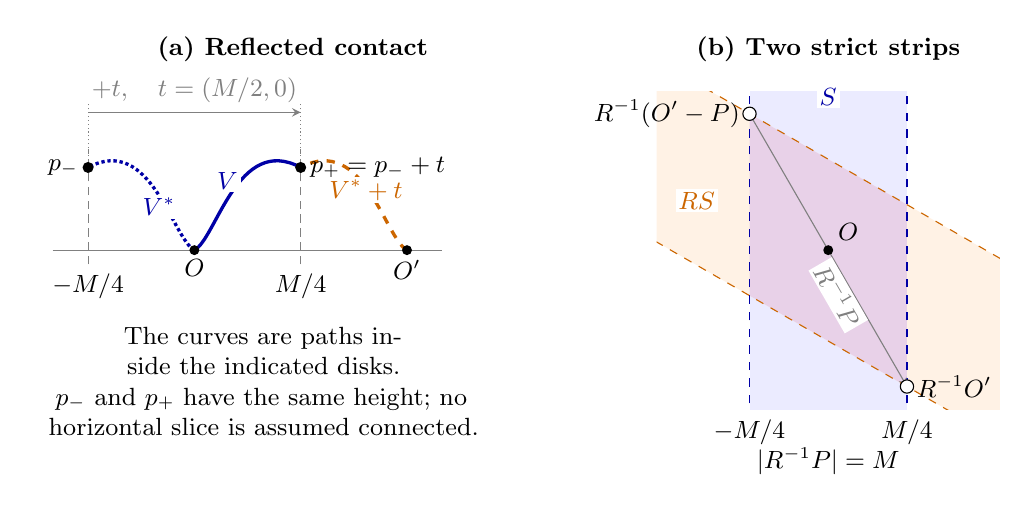
\begin{tikzpicture}[x=1cm,y=1cm,>=stealth,font=\small]
 \begin{scope}[shift={(2.4,0)}]
  \node[font=\small\bfseries] at (1.25,2.55) {(a) Reflected contact};
  \draw[gray] (-1.8,0)--(3.15,0);
  \draw[densely dashed,gray] (-1.35,-.18)--(-1.35,1.28);
  \draw[densely dashed,gray] (1.35,-.18)--(1.35,1.28);
  \draw[very thick,blue!65!black]
    (0,0) .. controls (.28,.15) and (.55,1.48) .. (1.35,1.05);
  \draw[very thick,blue!65!black,densely dotted]
    (0,0) .. controls (-.28,.15) and (-.55,1.48) .. (-1.35,1.05);
  \draw[very thick,orange!80!black,dashed]
    (2.7,0) .. controls (2.42,.15) and (2.15,1.48) .. (1.35,1.05);
  \draw[densely dotted,gray] (-1.35,1.05)--(-1.35,1.85);
  \draw[densely dotted,gray] (1.35,1.05)--(1.35,1.85);
  \draw[->,gray] (-1.35,1.75)--(1.35,1.75)
    node[midway,above] {$+t,\quad t=(M/2,0)$};
  \fill (0,0) circle (1.8pt) node[below] {$O$};
  \fill (2.7,0) circle (1.8pt) node[below] {$O'$};
  \fill (-1.35,1.05) circle (2pt)
    node[left] {$p_-$};
  \fill (1.35,1.05) circle (2pt)
    node[right] {$p_+=p_-+t$};
  \node[below] at (-1.35,-.18) {$-M/4$};
  \node[below] at (1.35,-.18) {$M/4$};
  \node[blue!65!black,fill=white,inner sep=1pt] at (.42,.88) {$V$};
  \node[blue!65!black,fill=white,inner sep=1pt] at (-.45,.55) {$V^*$};
  \node[orange!80!black,fill=white,inner sep=1pt] at (2.18,.76) {$V^*+t$};
  \node[anchor=north,align=center,text width=5.7cm] at (.85,-.85)
    {The curves are paths inside the indicated disks.\\
     \(p_-\) and \(p_+\) have the same height; no horizontal
     slice is assumed connected.};
 \end{scope}
 \begin{scope}[shift={(10.45,0)}]
  \node[font=\small\bfseries] at (0,2.55) {(b) Two strict strips};
  \begin{scope}
   \clip (-2.18,-2.02) rectangle (2.18,2.02);
   \fill[blue!8] (-1,-3) rectangle (1,3);
   \begin{scope}[rotate=60]
    \fill[orange!10] (-1,-3) rectangle (1,3);
   \end{scope}
   \fill[violet!18]
     (1,.57735)--(1,-1.73205)--(-1,-.57735)--(-1,1.73205)--cycle;
   \draw[blue!65!black,dashed] (-1,-3)--(-1,3);
   \draw[blue!65!black,dashed] (1,-3)--(1,3);
   \begin{scope}[rotate=60]
    \draw[orange!80!black,dashed] (-1,-3)--(-1,3);
    \draw[orange!80!black,dashed] (1,-3)--(1,3);
   \end{scope}
  \end{scope}
  \draw[->,gray] (-1,1.73205)--(1,-1.73205)
    node[pos=.64,sloped,below,fill=white,inner sep=1pt] {$R^{-1}P$};
  \fill (0,0) circle (1.8pt) node[above right] {$O$};
  \draw[fill=white] (-1,1.73205) circle (2.4pt)
    node[left] {$R^{-1}(O'-P)$};
  \draw[fill=white] (1,-1.73205) circle (2.4pt)
    node[right] {$R^{-1}O'$};
  \node[blue!65!black,fill=white,inner sep=1pt] at (0,1.95) {$S$};
  \node[orange!80!black,fill=white,inner sep=1pt] at (-1.67,.63) {$RS$};
  \node[below] at (-1,-2.03) {$-M/4$};
  \node[below] at (1,-2.03) {$M/4$};
  \node at (0,-2.68) {$|R^{-1}P|=M$};
 \end{scope}
\end{tikzpicture}

\caption{The two planar constructions in the escape bound.
In (a), only connecting paths inside \(V\), \(V^*\), and \(V^*+t\)
are drawn; the two marked points at a common height establish the contact without
asserting that a horizontal slice is connected. In (b),
\(S=\{|x_{\rm horiz}|<M/4\}\) and \(RS\) are the two open strips.
The open circles are adjacent rotated-back lifts of the opposite mark.
Their separation is \(M\), the long diagonal of the strip intersection.
The paths in (a) are schematic; (b) is drawn to scale.}\label{j:fig-localization}
\end{figure}

Now let \(U\) be nonwide and have diameter greater than \(CM\). It is
contained in the strict strip \(S=\{|x_{\rm horiz}|<M/4\}\). Let \(R\)
be rotation by \(\pi/3\) about \(O\). Although this rotation is not an
automorphism of the cylinder, \(RU\) projects to an embedded disk on
the same cylinder. Indeed
\[
 R^{-1}P=(M/2,-\sqrt3M/2),
\]
and the strips \(S\) and \(S+kR^{-1}P\) are disjoint for every nonzero
integer \(k\). Hence \(RU\) is disjoint from all its nontrivial period
translates. Moreover
\[
 \bigl(R^{-1}(O'+kP)\bigr)_{\rm horiz}=M/4+kM/2
\]
lies outside \(S\) for every integer \(k\). The projected disk therefore
encloses \(O\) and excludes \(O'\). Rotation preserves the honeycomb
graph and the weight. It is injective on this class because the image
disk has a unique lift containing the origin.

For any two such disks \(U,V\), compatibility of the boundaries of
\(U\) and \(RV\) would force one disk strictly inside the other.
The inner disk would then lie in \(S\cap RS\). The closure of this
intersection is a parallelogram with diagonals \(M\) and \(M/\sqrt3\);
in particular its diameter is \(M\), as shown in
Figure~\ref{j:fig-localization}(b). Both candidate inner disks have
diameter greater than \(CM>M\), a contradiction. Every original/image
pair is incompatible, so the weight \(S_L\) of this nonwide large class
satisfies
\[
 S_L^2\le I_M.
\]
Translation by \(t\) gives the identical two estimates for disks
enclosing \(O'\).

It remains to handle noncontractible cycles. Each simple
noncontractible cycle separates the two ends of the infinite cylinder.
Two disjoint such cycles are vertically ordered: after compactifying
the two ends, this is the nesting order of two disjoint curves
separating the two added points. Divide the cycles that separate the
marks into two classes according as \(O\) lies in their upper or lower
component. A cycle in one class is incompatible with every cycle in
the other, since disjoint vertically ordered cycles cannot reverse the
order of \(O,O'\). Reflection in the horizontal line interchanges the
classes and preserves weight. If each class has weight \(s\), their
ordered cross-pairs give \(I_M\ge2s^2\). Their combined weight is
therefore at most \(\sqrt{2I_M}\).

The two wide classes, the two nonwide large classes, and the
noncontractible classes are disjoint and exhaust \(\mathcal E_M\).
Their bounds sum to
\[
 2\sqrt{8I_M}+2\sqrt{I_M}+\sqrt{2I_M}
   =(5\sqrt2+2)\sqrt{I_M}.
\]
Outside these classes a disk contains its marked lift and has diameter
at most \(CM\), so every point in it is within distance \(CM\) of that
mark.
\end{proof}

We now compare the cylinder partition with \(\mathcal Z\), the planar
\(+2\) nesting partition defined in Section~\ref{c7:boundary}.
At fugacity \(2\), dropping every disjointness constraint involving
\(\mathcal E_M\) costs at most
\[
 \prod_{\lambda\in\mathcal E_M}(1+2w_\lambda)
 \le \exp\left(2\sum_{\lambda\in\mathcal E_M}w_\lambda\right)
 =\exp(O(\sqrt{\log M})).
\]
Every remaining disk lift lies in a ball of radius \(CM\). A regular
tessellation hexagon of side \(\lceil C'M\rceil\), for fixed
\(C'>2C/\sqrt3\), contains this ball. Same-mark disjointness is
preserved on the chosen lifts. Dropping constraints between the two
marks therefore bounds the remaining partition by the product of the
two corresponding planar partitions.

For the reverse comparison fix \(0<c<1/4\). Hexagons of side
\(\lfloor cM\rfloor\) about the two marked lifts, together with all
their period translates, are pairwise disjoint for large \(M\).
Their surrounding cycles project to separating cylinder cycles with
all joint disjointness preserved. We have proved
\[
 \mathcal Z(\lfloor cM\rfloor)^2
 \le G_{A,B}(2)
 \le \mathcal Z(\lceil C'M\rceil)^2
       \exp(O(\sqrt{\log M})).
\]
The cylinder estimate \(G_{A,B}(2)=M^{1/6+o(1)}\) now gives
\(\mathcal Z(R)=R^{1/12+o(1)}\). To pass from the displayed arguments
to every integer \(R\), use monotonicity of \(\mathcal Z\). For its upper
bound choose the least multiple \(M\) of \(4\) with
\(\lfloor cM\rfloor\ge R\); for its lower bound choose the greatest
multiple \(M\) of \(4\) with \(\lceil C'M\rceil\le R\).
These choices differ from \(R/c\) and \(R/C'\), respectively, by
bounded additive amounts.

Substituting this nesting exponent in the bounds for the mean in
Section~\ref{c7:boundary} gives
\[
 \mathbb E_R^{\rm chord}N=R^{4/3+o(1)}.
\]
For the bulk-visit conclusion, Proposition~\ref{j:visit} compares the
ordinary visit mass with \(\sum_{f\sim v}Z_D(f)\) by
\eqref{j:visit-identity} and \eqref{j:incident-face-partition}.
The domain inclusions following that proposition therefore give,
uniformly for honeycomb vertices \(v\) at distance at most \(R/10\)
from the center,
\[
 c\mathcal Z(\lfloor R/2\rfloor)
 \le \mathcal V_R(v)\le C\mathcal Z(3R)
\]
for all sufficiently large integer \(R\). Using the chord normalization
\eqref{j:chord-partition}, we obtain
\[
 \mathbb P_R^{\rm chord}(v\in\gamma)
   =\frac{\mathcal V_R(v)}{Z_R^{\rm chord}}
   =R^{-2/3+o(1)}
\]
uniformly in the stated range. This proves the mean and bulk-visit
conclusions of Theorem~\ref{j:hexagon}.

\section{Two marked bonds on tilted cylinders}\label{c7:marked}

The length-square estimate in \eqref{j:polygon-square} will follow by
summing the weight of polygons through pairs of specified bonds. We
first represent that positive sum by a finite matrix element. The
quantitative estimate allows the two intervals between the bonds to
have different lengths.

\subsection{The physical sum and the estimate to prove}

Put $\tau=e^{i\pi/3}$. After a lattice rotation or reflection, a
\emph{permitted cut} is a periodic path of tessellation sides whose
steps are $1$ and $\tau$. Translating it by the time step $\tau^2$
gives rows of rhombi: the spatial projection transverse to $\tau^2$
is strictly increasing, so these rows tile the plane. A period has
$M$ sides and a nonzero lattice translation $P$. We call a site
horizontal when its cut step is $1$, and mark the honeycomb bond
crossing each of two horizontal sites $i,j$. Choose the seam just
before $i$. The period then consists of consecutive nonempty lists
$A,B$, with $i$ first in $A$ and $j$ first in $B$; write
$A'=A\setminus\{i\}$ and $B'=B\setminus\{j\}$.

On the cylinder modulo $P$, let $H^{\rm poly}$ be the increasing
closed-rim height limit of
\[
 \sum_{\substack{\lambda\ {\rm a\ single\ simple\ unoriented\ cycle}\\
                   \lambda\ {\rm uses\ both\ marked\ bonds}}}
 x^{|\lambda|}.
\]
The sum includes contractible and noncontractible cycles. The
proposition below proves that the limit is finite.

The associated physical site variables have shifted-to-horizontal
ratio $q=e^{i\pi/4}$. Indeed the angles of the two rhombi relative
to the time step are $\pi/3$ and $2\pi/3$; at one common physical
row their spectral differences are $\alpha$ and $2\alpha$ for the
shifted and horizontal sites, respectively. At both differences
the scalar weights are exactly the honeycomb weights after splitting
each rhombus into two equilateral triangles. At $2\alpha$ the
weights $u,d$ and $a,b$ are interchanged relative to $\alpha$.

For a generic nonzero site list $X$ on the same two lists, define a
separate algebraic quantity
\begin{equation}\label{j:marked-flip-definition}
 H^{\rm flip}(X)=
 L_- f_i\, i^{\sum_{a\in A'}s_a^{\rm phys}} e_j R_+,\qquad
 f_i=|-\rangle_i\langle+|,\quad e_j=|+\rangle_j\langle-|.
\end{equation}
Here $s_a^{\rm phys}$ is the diagonal site-spin operator, and
$R_+=R_i$, $L_-=L_{-i}$ are the selected vacuum vectors of
Lemma~\ref{j:selected-vacuum-vectors}. Their generic normalization
is the one fixed in Section~\ref{c7:finite}.

\begin{proposition}[Physical two-bond identity]\label{j:marked-physical}
Let the permitted cut have even $M$, and let both marked sites be
horizontal. The positive sum $H^{\rm poly}$ is finite. The generic
matrix element $H^{\rm flip}$ has a regular limit at the associated
physical site list, and at that list
\[
 H^{\rm flip}=H^{\rm poly}.
\]
This holds for every order and every number of the two site types in
the two nonempty lists; the unmarked lists may be empty.
\end{proposition}

\begin{theorem}[Unequal marked intervals]\label{j:unequal}
Use the physical tilted cylinder and horizontal-type marked bonds
just defined. Its two cut intervals have $m+1$ and $n+1$
sites, with $n\ge m$ and $M=m+n+2$ even. In each unmarked list the logarithmic site
coordinates have imaginary parts $-f$ and $1-f$, where $0\le f\le0.6$. Their respective
counts differ from $m(1-f),mf$ in the first unmarked list and from
$n(1-f),nf$ in the second by at most a fixed constant. Let $H^{\rm poly}$
be the sum of $x^{|\lambda|}$ over single unoriented polygons through
the two specified bonds. Uniformly over these lists and their orders, for
every $\epsilon>0$ there are $C_\epsilon$ and $m_\epsilon$ such that
\[
 H^{\rm poly}\le C_\epsilon n^\epsilon m^{-4/3}(n/m)^{1/3}
 \qquad(n\ge m\ge m_\epsilon).
\]
Both $C_\epsilon$ and $m_\epsilon$ may depend on the fixed bound for
the count discrepancies.
\end{theorem}

The physical identity has the broader domain: its proof uses the
selected vacuum vectors, a finite nonvanishing result for their scalar
normalizer, summability on a fixed cylinder, and a two-arc phase
calculation. The count restrictions in Theorem~\ref{j:unequal} enter
later, when Sections~\ref{c7:markedgas}--\ref{c7:mixed} estimate the
horizontal representation. We keep the algebraic and positive sums
separate until Proposition~\ref{j:marked-physical} is proved.

\subsection{The generic flip formula}

Put $U=x_i$, $V=x_j$, and retain arbitrary nonzero values of these
variables. For the unmarked lists $(A',B')$, let $C_s$ denote the
summand in \eqref{j:finite-spin-sum} for $N^2\mathscr G$ at $h=1$,
including its phases. Thus the labels satisfy
$Q=\sum_{A'}s_a=\sum_{B'}s_a$. For a pair $(u,v)$ write
$e_k(u,v)=v-q^k u$.

\begin{proposition}[Generic long-flip formula]\label{j:marked-flip-formula}
For generic nonzero $X$ on consecutive nonempty lists $A,B$,
\begin{equation}\label{c7:eq-L}
\begin{aligned}
 N(X)^2 H^{\rm flip}(X)
 &=cUV\sum_s q^{-6Q}C_s
       \prod_{a\in A'\cup B'}F_{s_a}(U,x_a)F_{s_a}(V,x_a),\\
 (F_+,F_0,F_-)&=(e_5e_6,e_3e_5,e_2e_3),\qquad c=2-\sqrt2.
\end{aligned}
\end{equation}
The two endpoint variables $U,V$ are independent in this identity.
\end{proposition}

\begin{proof}
We first separate the individual spin terms of the unflipped pairing.
For each of two lists, use its ordered partial monodromy with both
auxiliary ends fixed at $+1$ for the first list and at $-1$ for the
second. Within a list these operators commute as the probe varies:
the exchange proof applies because the equal extremal auxiliary pair
has a scalar block. Label basis spins by $s=s^{\rm phys}$ in the
first list and $s=-s^{\rm phys}$ in the second. At fixed total spin,
order configurations by their prefix sums. Each partial monodromy is
triangular, with row $\le$ column, because the intermediate auxiliary
spin stays within its bounds.

The diagonal characters are products of the one-site entries
$r_s(w/x)$, where
$(r_+,r_0,r_-)=(a_{\rm tile},v_{\rm tile},b_{\rm tile})$.
They are distinct jointly at generic variables. Their denominator
roots are $w/x=q^5,q^6$, and their numerator root indices are
\[
D_-=\{0,1\},\quad D_0=\{0,3\},\quad D_+=\{2,3\}.
\]
Apply the joint eigenprojection to its leading coordinate to obtain
$|s\rangle\rangle$ and $\langle\langle s|$, taking the product over
the two lists. Their leading coefficients are one, their ket and bra
supports are respectively $\le s$ and $\ge s$, and they are dual.
Indeed each generic projection is a polynomial in triangular matrices
with exactly one diagonal entry equal to one.

Consider the two amplitudes $N\langle\langle s|R_+$ and $N L_- |s\rangle\rangle$, in total physical charge zero. We list forced factors, omitting phases. In both there is a factor $\prod_a x_a^{s_a^2/2}$. For a same-group pair in order $x,y$, labels $a,b$, the right amplitude (involving $R_+$) has zeros
\begin{itemize}
\item $e_5(x,y)$ unless $(a,b)=(+,-)$;
\item $e_6(x,y)$ unless $(a,b)\in\{(+,0),(0,-),(+,-)\}$.

\end{itemize}
Allow denominator $e_0$ if $a<b$, $e_1$ for $(-,+)$, $e_7$ for $(0,0)$. For the left amplitude use the same right rule with the order reversed. Thus the product of the two rules gives the rational monic part of $p_{ab}$ above up to constants. For a cross pair (either list first), in \textbf{each} amplitude use a factor $e_5$ if $a<b$, $e_3$ if $a>b$, additionally $e_6$ for $(-,+)$, $e_2$ for $(+,-)$. There are no cross denominator factors.

\paragraph{Forced factors and partial spectra.}
The vacuum input here is precisely the asymmetric statement of
Lemma~\ref{j:selected-vacuum-vectors}. For a physical zero-charge
configuration $\sigma$ and $t_a^2=x_a$, it says that
\[
 \frac{N(R_+)_\sigma}{\prod_a t_a^{\sigma_a^2}},
 \qquad
 \frac{N(L_-)_\sigma}{\prod_a t_a^{\sigma_a^2}}
\]
are polynomials in the ordinary site variables, independent of the
square-root signs, of degree at most $|X|-1-\sigma_a^2$ in $x_a$.
For a vacant coordinate, their value at $x_a=0$ is
$\prod_{b\ne a}x_b$ times the corresponding reduced polynomial,
and their coefficient of $x_a^{|X|-1}$ is that reduced polynomial.
With one varied site and generic fixed spectators, the proof also
gives, for the normalized coordinates, an occupied coordinate of
order $O(t_a)$ at zero and $O(t_a^{-1})$ at infinity, and the
reduced vacant coordinate at both limits. These conclusions apply
to $R_+$ and $L_-$ only.

The additional poles of our amplitudes come from the partial
projections. At a generic point of a same-list divisor
$y=q^\delta x$, their spectral coincidences require equality of
$D_a\cup(\delta+D_b)$ modulo 8 at fixed $a+b$. The displayed root
lists give only the following doublets: unequal swapped labels at
$\delta=0$; $(-,+)$ and $(0,0)$ at $\delta=1$; and their reflections
at $\delta=-1$. The spectator labels agree, and there are no
coincidences at other generic divisors. A regular generic linear
combination of probes separates either doublet to first order:
moving the second ratio moves a different multiset of numerator
roots, so the logarithmic derivatives differ. It also separates
the other characters. Thus these poles have order at most one.
Solving in triangular order on supports shows that the ket of the
lower label and bra of the higher have no pole, since those supports
exclude the colliding index. This is exactly the denominator rule
above. Several characters can coincide at an intersection of these
divisors; we make no doublet assertion there.

The singleton limits of the partial basis require a separate
observation. With one site on its own scale, fixed regular probes
have diagonal entry $q^{\pm3s}$ times the generic spectator
character, so a generic probe has a holomorphic simple projection
at that limit. It preserves the varied site's vacancy parity there.
Let $P_a$ act by $(-1)^{\sigma_a^2}$ on the physical site basis.
The leading-coordinate normalization gives
\[
 |s\rangle\rangle(-t_a)
   =(-1)^{s_a^2}P_a|s\rangle\rangle(t_a),\qquad
 \langle\langle s|(-t_a)
   =(-1)^{s_a^2}\langle\langle s|(t_a)P_a.
\]
Together with the coordinate limits of the selected vectors, this
shows that either amplitude divided by $N$ is bounded at both
singleton ends, and is respectively $O(t_a)$ and $O(t_a^{-1})$
there if $s_a=\pm1$. It also shows that extracting
$\prod_a t_a^{s_a^2}$ makes each amplitude rational in the ordinary
variables.

For same-group fusion put a higher site $q^\delta u$ before a lower $u$, $\delta=2,3$. The site intertwiner used above places $R_+$ in its image and intertwines even the partial monodromy there (for adjacent sites). Simplicities of the full and reduced fixed characters hold generically there by the same paired-scale tests, and the partial spectra are still simple by the root lists. Only labels realizing a reduced eigenvalue can occur in $\langle\langle s|R_+$. Comparing numerator lists after denominator cancellation, in (high, low) order these are $(+,-)$ for $\delta=3$, and $(+,0),(0,-),(+,-)$ for $\delta=2$. For instance at $\delta=2$ the two removed poles in numerator indices relative to $u$ are $0,5$. This proves the same-group right zeros. Swaps moving the pair together while preserving their relative order are allowed by regular exchange similarities at generic spectators, mapping the partial label projections along with the fixed lines. The normalizations cause only nonzero finite scalars (all these lines simple with their stated leading coefficients). The identical reasoning in reversed order proves left zeros: at real phases take Hermitian adjoints of monodromies, which reverses order (and conjugates the twist), then extend identities algebraically.

For cross fusion with $x=q^\delta y$, put the high site last of its list and the low first of its list. This uses same-list swaps, and, if the lists have to be interchanged cyclically, a seam change acting by a diagonal twist on the conserved list spin (hence preserving partial eigenspaces), directly by charge conservation. Suppose first the high site is in the first ($+$ convention) list. In the right-amplitude bra its physical spin is $\le a$ by prefix support; that of the low site is $\le-b$. But the vacuum ket in the fusion image uses total spin on the pair equal to 0 at $\delta=3$, or in $[-1,1]$ at $\delta=2$. This excludes $a<b$ or $a<b-1$ respectively. When the high site belongs to the other list negate physical spins in this argument. Apply the same adjacency arrangement in reversed order to the adjoint for the left amplitude. This proves the claimed cross factors, with both signs of shifts by interchanging arguments.

After dividing by the stated rational factors and site half powers,
the remaining rational function has no pole. Indeed every possible
irreducible divisor at finite nonzero values has been checked at a
generic point, and the singleton parity estimate removes the
possible pole at zero. Unique factorization then removes the same
denominators globally, including at intersections of shifted
divisors. The remainder is a polynomial. For a pair, the net degrees
used by the rational factors are $1+st$ in the same list and
$1-st-\mathbf1_{s=t=0}$ across lists. Charge equality, the
singleton bounds, and $\deg_{x_a}N\le |X|-1$ show that this
polynomial is independent of every nonzero-label variable. Its
degree in a zero-label variable is at most the number of zeros in
the opposite list.

It follows that individually for the unflipped two-list problem
\[
N^2\, i^Q(L_- |s\rangle\rangle)(\langle\langle s|R_+) = C_s
\]
(here $C_s$ and $Q$ temporarily refer to those arbitrary lists). Indeed induct on size. If a list has a distinct-label pair, choose a specialization $(x,y)=(u,q^2u)$ on these labels in \emph{ascending label} order (regardless of site order). This imposes a value on a nonzero-label variable, still free in the factored-out portion, without any zero or pole from its forced factors. By full similarity covariance of the left-right projected product (normalization by vacuum overlap 1), we may arrange the high site immediately before the other (same-list reordering here is an identity first at generic coordinates, continued to the regular values on this specialization even if an exchange itself becomes singular). Site fusion now reduces the cleared expression exactly to the reduced individual label expression times the $N^2$ fusion multiplier: the right fixed vector lies in the image, the partial probes intertwine there with simple spectra, the left fixed vector restricts to the reduced one up to normalization (product of normalizing scalars 1 by overlap), and the list spin is unchanged. The product check for surviving summands in the earlier spin formula has precisely this individual reduction. The displayed candidate shares the rational/degree rules (with the extra cross $00$ numerator), so the single evaluation in the nonzero-label variable proves equality. This handles all nonuniform cases. The remaining cases then follow by summing projections and comparing coefficients of $h^Q$ in the known unflipped spin sum: the all-zero term is the only unaccounted one there at $Q=0$, and a uniform charged configuration, if any, uniquely realizes its extremal $Q$ on two equal nonempty lists. This includes the induction base.

\paragraph{Insertion of the two long flips.}

Insert now the long flips between expansions in the partial bases on the \textbf{full} lists. By first-site triangular support the matrix element from ket label $v$ to bra label $u$ is zero unless $v_i=v_j=+$ and $u_i=u_j=-$. In these branches (physical first spins necessarily extremal due to the flips), the sections of basis vectors at their indicated first labels are exactly the corresponding normalized partial basis vectors on the remaining lists: the fixed-first-label triangular diagonal block of the probes is just the reduced probe times that first diagonal factor. Thus remaining labels have to match, say $s$ there, and the matrix element equals $i^Q$. We must evaluate $N^2(L_-|u\rangle\rangle)(\langle\langle v|R_+)$ with these labels. As functions of $U,V$ the forced factors and degree rule determine this up to a spectator factor: multiplying the two tables gives precisely
\[
UV\prod_a F_{s_a}(U,x_a) F_{s_a}(V,x_a)
\]
for their entire dependence (product over unmarked sites). Here the endpoints were first of their own lists.

Put the endpoints now together on one large scale above the spectators, in generic ratio. In these particular amplitudes $|u\rangle\rangle$ and $\langle\langle v|$ have actual first spins fixed by extremality, and reduced-list sections as just noted. Their physical endpoint total charge is zero, so only the diagonal grade block of the vacuum projections is needed. The two-scale argument above isolates the fixed character as a product of endpoint pair and spectator projections, up to the common diagonal similarity: charged endpoint totals are excluded exactly by the regular pair tests used for matched pair scales ($p_j^{S_j}$ for odd total, and the generic scalar $p_j^{\pm1}a_{\rm tile}$ for absolute total two). Neutral blocks see original twists. On endpoint physical spins $(t,-t)$ and given spectator list totals $(Q,-Q)$ the similarity displayed there acts by $q^{3tQ}$. Hence the amplitudes divided by $N$ each pick up $q^{3Q}$ relative to the reduced-list ones in this limit, as well as the endpoint pair components, whose combined multiplier by the explicit vacuum pair formula ($p=i$ on right, $-i$ on left, respectively entries $+,-$) is $cUV/(U+V)^2$. Also
\[
N(X)\sim (UV)^{|X|-2}(U+V) N(X\setminus\{U,V\});
\]
cross rows in the Pfaffian coincide toward the rest. Finally the leading phase in the displayed $F$ product is $q^{6\sum_a s_a}=q^{12Q}$. This computes the spectator factor by the individual unflipped formula and proves \eqref{c7:eq-L}.
\end{proof}

\subsection{Finite nonvanishing at the physical sites}

The physical vacuum argument needs only finite nonvanishing. The
growth of the same scalar with the number of sites will enter later
in Section~\ref{c7:markedgas}.

\begin{lemma}[Orbital ratio and nonvanishing]\label{j:shifted-nonvanishing}
Let $M=2L\ge2$, $w_j=i h_j$ with $h_j\in\mathbb R$ of spread at
most one, and $x_j=e^{\eta w_j}$, where $\eta=\pi/4$. Define
\[
 \mathcal S(X)=\mathcal P(X)\prod_{j<l}C(w_j-w_l),
 \qquad C(r)=\tanh(\pi r/6),
\]
using the confluent value for equal sites. Then $\mathcal S(X)\ne0$
and
\begin{equation}\label{j:shifted-orbital-ratio}
 \frac{N(X)}{\mathcal S(X)}
 =\left(\frac23\right)^L
   \mathbb E_h\exp\!\left(\sum_{a=1}^L\phi(k_a)\right)>0,
 \qquad
 \phi(k)=\log\left(1+\frac{e^{-2k}}{1+e^{-4k}}\right).
\end{equation}
Here $\mathbb E_h$ has ordered density on $0<k_1<\cdots<k_L$
proportional to
\[
 \Delta(k^2)^2\prod_{a=1}^L\frac{k_a}{\sinh3k_a}\ I_h(k),
 \qquad
 I_h(k)=\int_{U(2L)}
     e^{\operatorname{tr}(D_k\mathcal U D_h\mathcal U^*)}\,d\mathcal U,
\]
where $D_k=\operatorname{diag}(k_1,\ldots,k_L,-k_1,\ldots,-k_L)$
and $D_h=\operatorname{diag}(h_1-h_*,\ldots,h_M-h_*)$ for
$h_*=(\max h_j+\min h_j)/2$. The measure on $U(2L)$ is normalized
Haar measure. In particular $N(X)\ne0$. The nonvanishing also holds
after multiplying every $x_j$ by the same nonzero scalar.
\end{lemma}

\begin{proof}
First, each pair factor
$d(x_j,x_l)C(w_j-w_l)/(x_j-x_l)$ is nonzero on this domain,
including its finite nonzero limit at equality. Indeed the roots of
$d(u,v)=u^2+\sqrt2uv+v^2$ have relative arguments
$\pm3\pi/4$, outside the present range $[-\pi/4,\pi/4]$.
Within $|\Im(w_j-w_l)|\le1$, the only zero of $C$ is the simple
zero at equality and $C$ has no pole. This proves the assertion
about $\mathcal S$.

For distinct $h_j$, use the transforms of $B_0'$ and $C'$ in the
homogeneous normalization calculation. For either odd kernel
$B=B_0,C$,
\[
 B(i(h_j-h_l))
 =\int_0^\infty
   \frac{i\sinh((h_j-h_l)k)}{\pi k}\widehat{B'}(k)\,dk.
\]
The $L$th exterior power of the integral of these decomposable
two-forms expresses its Pfaffian as an integral of
$\det[e^{\pm h_j k_a}]$ on ordered positive $k_a$, with the product
of the corresponding weights $\widehat{B'}(k_a)/k_a$ and common
constants. Apply the unitary orbital determinant identity derived
before \eqref{j:boundary-orbital-law}. The Vandermonde of the paired
$k$ list supplies a constant times
$\prod_a k_a\,\Delta(k^2)^2$. Schur's identity gives
$\operatorname{Pf}C(w_j-w_l)=\prod_{j<l}C(w_j-w_l)$, while
\[
 \frac{\widehat{B_0'}(k)}{\widehat{C'}(k)}
 =\frac23 e^{\phi(k)},\qquad
 \widehat{C'}(k)=\frac{6k}{\sinh3k}.
\]
Taking the ratio proves \eqref{j:shifted-orbital-ratio}.

All integrations are absolute on the stated domain:
$\|D_h\|\le1/2$ gives $I_h(k)\le e^{\sum_a k_a}$, whereas
$k/\sinh3k$ decays like a polynomial times $e^{-3k}$.
This bound also permits coincident $h_j$ by continuity in the
orbital formula. The expectation is strictly positive at every
size, proving $N\ne0$. Homogeneity of $N$ and $\mathcal S$ gives
the last assertion.
\end{proof}

\subsection{Summability on a fixed cylinder}

\begin{lemma}[Period exclusion]\label{j:period-excluded}
Fix a nonzero lattice translation $P$ and a honeycomb vertex $v$.
The total critical weight of plane SAWs starting at $v$ whose
visited vertices are distinct modulo $P$ is finite. The empty walk
may be included. The bound may depend on $P$.
\end{lemma}

\begin{proof}
Rotate the lattice and, if necessary, replace $P$ by $-P$ so that
$P=a\tau+b(\tau-1)$ with integers $a,b\ge0$. These choices are
possible because the sixty-degree cones spanned by successive
lattice directions cover the plane. Use horizontal tessellation
lines for these coordinates. Let $a_h$ be the total weight of
first-exit slab crossings from a fixed bottom port to any top port
$h$ layers above, and let $b_h$ be the weight of those crossings
with no intermediate level crossed exactly once. The convex balance
in Section~\ref{j:local}, exhausted horizontally, gives
$a_h\le\csc(\pi/8)$ for every $h$.

Cut a crossing at every intermediate level that it crosses exactly
once. The resulting blocks are irreducible crossings counted by the
$b_h$. Conversely, any word of such blocks concatenates freely:
the first-exit property places successive blocks in disjoint open
slabs, sharing only their joining port. Their weights multiply.
Thus, for $0<t<1$,
\[
 A(t):=\sum_{h\ge1}a_ht^h
   =\sum_{r\ge1}B(t)^r<\infty,\qquad
 B(t):=\sum_{h\ge1}b_ht^h.
\]
It follows that $B(t)<1$ and, by monotone convergence,
$\mu:=\sum_{h\ge1}b_h\le1$.

Among the height-one blocks, choose the word that takes the $a+b$
upward moves whose sum is $P$ and then repeats its first block.
Its length is $r_P=a+b+1$ and its weight is
$p_P=x^{2r_P}>0$: each move traverses two triangles. Its first and
last repeated blocks visit vertices equal modulo $P$. A
period-excluding word must therefore avoid this specified word.
Divide any longer word into disjoint chunks of length $r_P$ and a
last shorter chunk. The sum of weights of words that avoid the
specified word is at most
\[
 \sum_{j=0}^{r_P-1}\mu^j
       \sum_{r\ge0}(\mu^{r_P}-p_P)^r
 \le \frac{r_P}{p_P}<\infty.
\]
The same remains true if a first and a last irreducible block are
left unrestricted, since their total masses are at most $\mu$.

We transfer this bound from ports to vertices. Measure a vertex
span $l$ in units of one third of the layer spacing. Extend a
segment whose endpoints are opposite height extrema to the adjacent
port lines, as in Lemma~\ref{j:extremal-segment}. The extension
adds at most one triangle at either end, at bounded multiplicity.
If the resulting slab has height $h$, then
$3h-l\in\{2,3,4\}$. The sequence of middle irreducible blocks
still belongs to the original period-excluding segment, so it
avoids the specified word. The preceding sum therefore gives
bounds $C_l$ for the weight of such segments from a fixed vertex to
all opposite extremal endpoints, with
\[
 \sum_{l\ge1}C_l<\infty.
\]
We take the maximum over both directions and the two vertex types;
the port extension costs only a fixed factor.

A segment starting at its highest vertex and staying no higher
splits at successive last opposite extrema as described after
Lemma~\ref{j:extremal-segment}. Its positive spans decrease
strictly, apart from a possible equality of the first two. Put
$d_l=C_l/x$, accounting for the shared vertex at a join. Summing
over these span lists costs at most a fixed factor times
\[
 \left(1+\sum_{l\ge1}d_l^2\right)
 \prod_{l\ge1}(1+d_l)<\infty.
\]
The empty segment is included. Finally split a full walk at a
specified highest vertex, for example the first such vertex. To
count the reversed first half without summing over free highest
positions, translate its highest endpoint to one of two fixed
representatives, according to vertex type. Its translated end and
the original fixed start determine the translation. Both halves
are therefore bounded by the preceding endpoint-summed bound.
\end{proof}

\subsection{The phase of two marked arcs}

We calculate phases on the reference flat cylinder with horizontal
cut and angle $\pi/3$, keeping the scalar weights of the physical
tilted rows. The local pictures and phases after the telescoping
removal in Section~\ref{j:local} are unchanged by this choice.
Place the seam at zero and write the endpoint abscissae as
$0<i<j<M$.

Consider a smooth regular embedded lift of one directed arc
$X:[0,1]\to\mathbb R^2$ from $(i,0)$ to $(j+kM,0)$,
$k\in\mathbb Z$, disjoint from all of its nontrivial horizontal
$M$-translates. Its endpoint tangents are vertical with signs
$\zeta_i,\zeta_j\in\{-1,1\}$, upward positive. Use a small
perturbation to make its interior cut and seam-ray crossings
transverse, retaining the absence of interior cut crossings at
seam or endpoint abscissae and its prescribed tangent turns.
The actual reference lattice arcs have this absence before
smoothing. Let $x_z$ and $\epsilon_z$ be the abscissae and signed
directions of the interior cut crossings, and define
\[
 \mu=\sum_{\text{interior crossings }z}\epsilon_z\delta_{x_z}
       +\frac{\zeta_i}{2}\delta_i
       +\frac{\zeta_j}{2}\delta_{j+kM},\qquad
 C(a)=\mu((-\infty,a))+\frac12\mu(\{a\}).
\]
The total mass is zero, since the interior signed crossing total is
$-(\zeta_i+\zeta_j)/2$. In particular $C$ has compact support.
Define the finite sums
\[
 C_0=\sum_{\ell\in\mathbb Z}C(\ell M),\qquad
 C_{\rm per}(a)=\sum_{\ell\in\mathbb Z}C(a+\ell M)-C_0.
\]
There is no interior crossing at a seam or an endpoint translate.
At an endpoint, $C$ includes half of an atom already of mass
$\zeta/2$, hence the contribution $\zeta/4$.

\begin{lemma}[Arc turn and seam count]\label{j:marked-phase}
Let $T(X)$ be the total turn of the lifted arc, and let $K$ be its
integer signed number of eastward crossings of the upper seam rays
$\{\ell M\}\times(0,\infty)$, summed over $\ell$. Then
\begin{equation}\label{j:marked-phase-identities}
 T(X)=-2\pi\bigl(C_{\rm per}(i)+C_{\rm per}(j)+2C_0\bigr),
 \qquad K=C_0+\frac{k}{2}.
\end{equation}
Consequently, for $q=e^{i\pi/4}$,
\[
 q^{4C_0}i^k(-1)^K=e^{2\pi iK}=1.
\]
\end{lemma}

\begin{proof}
For a seam or endpoint abscissa $a$, use the branch
$\arg(a-X)\in(0,2\pi)$. Each upward cut crossing
to the left of $a$ requires a correction $-2\pi$. The initial and
terminal branch arguments are respectively
\[
 \pi\bigl(1+\zeta_i\mathbf1_{i<a}\bigr),\qquad
 \pi\bigl(1-\zeta_j\mathbf1_{j+kM<a}\bigr),
\]
where an indicator is $1/2$ at equality. Thus the continuous
variation of $\arg(a-X(t))$, using one-sided endpoint limits, is
$-2\pi C(a)$.

Lift $\arg(X(t)-X(s))$ continuously on the triangle $s<t$.
On the route $(0,0)\to(0,1)\to(1,1)$, its changes are
$-2\pi C(i)$ and $-2\pi C(j+kM)$. On the diagonal its limiting
angle is the tangent angle, whose change is $T(X)$. The two routes
have the same endpoints, so
$T(X)=-2\pi(C(i)+C(j+kM))$. For $\ell\ne0$ instead lift
$\arg(X(t)+\ell M-X(s))$ on the whole square. Disjointness from
the translate makes this well defined. The diagonal angle is
constant; the same two-edge route therefore gives
\[
 C(i-\ell M)+C(j+kM+\ell M)=0.
\]
Summing these identities with the $\ell=0$ turn identity gives the
first formula in \eqref{j:marked-phase-identities}.

For a seam at $a$, let $I_a$ be the interior signed upward cut
flux to its left and let $K_a$ be the signed eastward crossings
of its upper ray. Flux from the upper-left region gives
\[
 K_a=I_a+\mathbf1_{\{\zeta_i=1,\ i<a\}}
          -\mathbf1_{\{\zeta_j=-1,\ j+kM<a\}}.
\]
Substituting the endpoint half-atoms into $C(a)$ makes this
\[
 K_a=
 C(a)+\frac{\mathbf1_{i<a}-\mathbf1_{j+kM<a}}2.
\]
An interior upward cut crossing enters that region and a
downward one leaves it; an upward start contributes $+1$, and
a downward finish contributes $-1$. Summing over $a=\ell M$
gives $K=C_0+k/2$, because
$0<i<j<M$ makes the sum of the indicator differences equal to
$k$. Here $K$ is an integer by its definition as a signed crossing
count. The displayed phase cancellation now follows by substituting
$C_0+k/2=K$.
\end{proof}

\subsection{Identification of the physical matrix element}

\begin{proof}[Proof of Proposition~\ref{j:marked-physical}]
For the physical site list, Lemma~\ref{j:shifted-nonvanishing}
gives $N\ne0$: after a common rescaling its logarithmic heights lie in
$\{0,1\}$, so their spread is at most one. Lemma~\ref{j:selected-vacuum-vectors} therefore
continues the selected vectors $R_+$ and $L_-$ componentwise to
this list, including its simultaneous coincidences. Their vacuum
components remain one, and the regular physical row matrices still
fix them.

We identify these algebraic vectors with the physical vacuum
limits. Stack the uniform-twist physical transfers, with twist
$i$ or $-i$, on the fixed cylinder modulo $P$. Untouched closed
loops cancel in the oriented sum. With any fixed rim states, the
remaining finitely many occupied rim ports are paired by oriented
arcs. The absolute weights of those arcs are bounded by products
of the period-excluding SAW sums of
Lemma~\ref{j:period-excluded}. Arcs reaching depth tending to
infinity from a rim have vanishing total weight, by the tail of
that finite sum. After discarding arcs that reach the middle row,
the bottom and top configurations occupy disjoint slabs and hence
factor. Thus, as the distance between the rims tends to infinity,
the transfer matrix factors into independent bottom and top vacuum
vectors. Their vacuum components are one. This
argument is for each fixed $P$ and needs no uniformity in its
length. Multiplying the continued fixed vectors by these large
powers identifies them, by their vacuum normalization, with the
corresponding physical vectors.

It remains to compute the finite-stack matrix element with the two
flips. On the reference geometry, the flips create two directed
arcs from $i$ to $j$, with opposite vertical signs at each
endpoint. Every other loop is disjoint from both arcs and cannot
separate the endpoints. Its interval insertion phase is therefore
one, so the usual orientation cancellation, including its seam
twist, removes it. The two arcs join to a single unoriented polygon.

For either arc, Lemma~\ref{j:marked-phase} makes its turning phase
\[
 e^{-iT(X)/4}
 =q^{2(C_{\rm per}(i)+C_{\rm per}(j)+2C_0)}.
\]
The total signed seam crossing count is $k$, and the signed upper
count is $K$. The lower twist $i$ and upper twist $-i$ thus
contribute $i^k(-1)^K$. Between the two arcs the endpoint atoms
cancel. Since the seam immediately precedes $i$, their summed
$C_{\rm per}(i)$ is zero. Physical spin counts downward crossings
positively, so the interval insertion equals
\[
 i^{\sum_{a\in A'}s_a^{\rm phys}}
 =q^{-2\sum_{\rm arcs}(C_{\rm per}(i)+C_{\rm per}(j))}.
\]
The remaining phase for each arc is
$q^{4C_0}i^k(-1)^K=1$. This holds for arbitrary integer $k$.
Each polygon has exactly the specified source-to-sink flow, so
its scalar weight is counted once and is $x^{|\lambda|}$.

The absolute arc sums above allow both rim heights to tend to
infinity in this finite-stack identity. They also prove finiteness
of the positive polygon sum. Hence
$H^{\rm flip}=H^{\rm poly}$ at the physical list.
\end{proof}

At a physical list we may henceforth write
$H_{\rm lg}=H^{\rm poly}=H^{\rm flip}$. At nearby generic lists
only $H^{\rm flip}$ is used. In particular any use of
\eqref{c7:eq-L} at a nongeneric list means the limit of its combined
expression. The next section estimates that algebraic quantity
before taking the physical limit.

\section{The horizontal representation with marked bonds}\label{c7:markedgas}

The marked matrix element changes the site source and adds one
varying angle. We first establish its horizontal gas identity for
finite lists at a supported finite period. We then continue the
identity to nearby shifted lists and send the period to infinity
with those lists fixed. The estimates uniform in their sizes and
orders come in Sections~\ref{c7:shifted} and \ref{c7:mixed}; only
after those estimates do we approach the physical spread-one
lists. The auxiliary site-count limit at fixed period used for the
mixed spectral radius is stated separately below.

\subsection{The endpoint source and the finite-list regulator}

Take the combined limit of \eqref{c7:eq-L} at
$U=V=e^{\eta w_e}$. This is the only specialization of its two
endpoint variables. Write
$W_\sigma=(w_{\sigma,1},\ldots,w_{\sigma,n_\sigma})$ for the
unmarked coordinates in species $\sigma=1,2$, with
$n_\sigma\ge0$, and set $x_{\sigma,a}=e^{\eta w_{\sigma,a}}$.
The full ordered list is $(U,e^{\eta W_1},U,e^{\eta W_2})$ and
has size $M=n_1+n_2+2$. Let $P_0(W_1,W_2)$ be the all-zero term
of the finite spin sum on the unmarked lists. Empty products have
value one.

The pair factors and sign cancellation for a defect
$\delta=-s=\pm1$ at centered coordinate $v=w+i\delta/2$ are
unchanged. Before Gaussian splitting, its potentials against a
zero site in the same and opposite species are respectively
\[
 V_{d,-}(w)=q^{-1}\frac{e_1e_7}{e_0e_6},\qquad
 V_{c,-}(w)=q\frac{e_3^2}{e_4^2},\qquad
 e_k=1-q^ke^{\eta w},
\]
and $V_{\rho,+}(v-i/2)=V_{\rho,-}(v+i/2)^{-1}$.
The local factor after sign cancellation is $\sqrt c$, before
these zero-site interactions. The extra $p_0/4$ in the matched
prescription came from the opposite-species zero at the same
coordinate.

The phase $q^{-6Q}$ and the two endpoint ratios in
\eqref{c7:eq-L} contribute $\exp(i\delta D_e(v-w_e))$ per defect,
where the odd branch $D_e$, real on the real line, is determined by
\[
 e^{-iD_e(v)}
 =q^{-3}\left(\frac{e^{\eta v}-q^{11/2}}
                    {e^{\eta v}-q^{5/2}}\right)^2.
\]
It is analytic on $|\Im v|<5/2$ and tends exponentially to
$\pm\nu$ at the two real infinities, where $\nu=3\pi/4$.
Indeed
\[
 D_e'(v)=\frac{2\eta\sin(5\pi/8)}
                  {\cosh(\eta v)-\cos(5\pi/8)},\qquad
 \widehat{D_e'}(k)=4\pi\frac{\sinh(3k/2)}{\sinh4k}.
\]

Fix $0<r<1/8$. Start with distinct real unmarked coordinates
and a real endpoint coordinate, all of absolute value less than $r/8$,
and take $T>8r$. Use the Gaussian and Wick data of
Section~\ref{c7:contour}. In the current
\eqref{c7:contour-current} of species $\sigma$, put $z=1$, use the
product of $U_{\delta,T}$ translated to its own list $W_\sigma$,
and use the circle $\gamma_r$ enclosing that list. Replace
$\varphi_\sigma(v)$ by $\varphi_\sigma(v)+d_T(v)$, where
\begin{equation}\label{j:marked-kink}
 d_T(v)=\sum_{\ell\in\mathbb Z}
 \bigl[D_e(v-w_e+\ell T)-D_e(v-w_e-T/2+\ell T)\bigr]-\nu.
\end{equation}
This function has zero mean, changes sign on translation by $T/2$,
and tends to $D_e(v-w_e)$ on compact sets as $T\to\infty$.
Call the resulting Wick current $\mathcal C^L_{\sigma,T}$.
With the zero-mean source
\[
 A_\sigma(x)=\sum_{w\in W_\sigma}a_T(x-w),\qquad
 A=(A_1,A_2)^t,
\]
define the normalized regulator
\begin{equation}\label{j:marked-regulator}
 \mathfrak C_T^L=
 \frac{\mathbb E\!\left[
 e^{i\int_T(DA)\cdot\chi}
 e^{-2\pi\sum_\sigma n_\sigma\ell_\sigma/T}
 \mathcal C^L_{1,T}\mathcal C^L_{2,T}\right]}
 {\mathbb E e^{i\int_T(DA)\cdot\chi}}.
\end{equation}
The source denominator is a nonzero Gaussian exponential.

\begin{proposition}[Fixed-list marked regulator]\label{j:marked-regulated-limit}
For every $T>8r$ and fixed finite initial lists and endpoint
coordinate as above,
the Wick expansion in species $\sigma$ terminates after order
$n_\sigma$ and extends to coalescing own lists in the same
neighborhood. As $T\to\infty$ with generic initial data fixed,
\begin{equation}\label{j:marked-regulator-limit}
 \mathfrak C_T^L\longrightarrow
 \frac{N(X)^2H^{\rm flip}(X)}
 {cU^2P_0(W_1,W_2)\prod_{a\in A'\cup B'}F_0(U,x_a)^2}.
\end{equation}
This statement is initially at values where the displayed
denominator is nonzero.
\end{proposition}

\begin{proof}
The current poles inside the contour are the simple poles at its
own sites. If two residues in one species select the same site,
their first Wick fields coincide and their Pfaffian vanishes.
The kink is analytic on these contours. The same fixed-contour
argument as in Proposition~\ref{c7:regulated-pfaffian} therefore
proves termination and continuation to coalescing lists. In
particular this is a finite residue calculation at each fixed
pair of lists.

Here is the changed one-site contraction. Put
$\mathfrak a_\rho(v)=\log V_{\rho,-}(v+i/2)$, using the odd
branch zero at $v=0$. These logs have step limits. At $k>0$,
their transforms in units $2\pi/k$ are
\[
 \frac{t^{1/2}(1-t)(1+t^6)}{1-t^8},\qquad
 -\frac{2t^{7/2}(1-t)}{1-t^8},\qquad t=e^{-k},
\]
for $\rho=d,c$. Differentiate the factors and use the
hyperbolic transform from Section~\ref{c7:contour}: the exponents
in $(0,8)$ are $1.5,7.5$ versus $.5,6.5$ for the first log, and
$3.5,3.5$ versus $4.5,4.5$ for the second. Integrating the
transforms symmetrically fixes their odd primitives. The resulting
column of transforms is
$(I+gE)(\widehat a,0)^t$.

At centered argument, the own-site $U$ translate contributes
$-\delta a$ to the logarithm. The normalized Gaussian source
contributes $-\delta G_{\sigma\sigma'}D a$ per site of species
$\sigma'$. Their sum is exactly $-\delta\mathfrak a_\rho$.
The other pair and constant-mode contractions are those already
proved; in particular the difference charge is neutral, so the
singular difference-channel covariance acts only on tests
vanishing at zero frequency. Symmetric Fourier sums for the step
primitive converge after differentiation and integration from
zero. At fixed lists the winding slopes and the compensation in
\eqref{j:marked-regulator} disappear in the large-period
Gaussian sum. The local residue is $\sqrt c$; multiplying it by
$V_{c,\delta}(0)=p_0/4$ recovers the earlier matched residue.
The finite residue terms are consequently exactly those in
\eqref{c7:eq-L} after its all-zero normalization. Their convergence
is locally uniform at the fixed generic initial data, proving
\eqref{j:marked-regulator-limit}.
\end{proof}

\subsection{The changed gas data}

Write
\[
 g_+=g_d+g_c,\qquad
 l(k)=\frac{kE(k)}{1+g_+(k)E(k)},\qquad L_*:=l(0)=\frac89.
\]
Let $y_T=\partial^{-1}d_T$ have zero mean. Define $J_T^{\rm loc}$
by applying the Fourier multiplier $(l(k)-L_*)/k^2$ to $d_T'$,
using its regular value at zero. This is a periodized difference
of translates to $w_e$ and $w_e+T/2$ of a fixed exponentially
decaying function. It is analytic at position heights of absolute
value less than $5/2$ relative to either center. These facts
follow by multiplying $\widehat{D_e'}$ by the displayed symbol:
the symbol is regular at zero and meromorphic with polynomial
growth on a narrow strip about the real frequency axis.

Use the six complete particle lists \eqref{j:particle-list}, the
fused union list \eqref{c7:fused-list}, and the state gas
\eqref{c7:gas-definition}, now at the fixed post-collision
displacement $d=1/8$. The residual pair factors, local activities,
state space, and charge jumps are those of that gas at this
displacement. Its changes are the following.

\begin{enumerate}
\item In each $H$ dress of species $\sigma$, replace $B_T(v)^m$
by $\prod_{w\in W_\sigma}B_T(v-w)$. These products use only that
species' unmarked list.
\item In the integral square of \eqref{c7:state-weight}, replace
$\theta$ by $d_T(x)$; in the local Berry phase of a particle at
$x_j$, replace it by $d_T(x_j)$.
\item For an $H$ entry at height $a'$ and center $x$, with signed
power $r$, add to its dress logarithm
\begin{equation}\label{j:marked-local-dress}
 r\left[J_T^{\rm loc}(x+ia')
  -L_*\bigl(y_T(x+ia')-y_T(x)-ia'd_T(x)\bigr)\right].
\end{equation}
\end{enumerate}

The last logarithms are bounded and exponentially localized near
the two kinks, for $|\Im w_e|\le0.6$ and the listed heights. They
are evaluated on every $H$ entry, preserving the listed internal
order and the analytic fused union value. In particular the fused
particle's kink multiplier is generally not one.

For later boundary evaluation, the site part of item 1 must first
be simplified by \eqref{c7:B-recurrences}. For a particle in
species $\sigma$ it is
\begin{equation}\label{j:marked-site-factors}
\begin{array}{c|l}
 P&\displaystyle\prod_{w\in W_\sigma}B_T(x-w)\\
 M,\ F_{\rm pair}&1\\
 O_+&\displaystyle\prod_{w\in W_\sigma}B_T(x-w-i)\\
 O_-&\displaystyle\prod_{w\in W_\sigma}B_T(x-w+i)\\
 U&\displaystyle\prod_{w\in W_\sigma}B_T(x-w+i(3/2+d))^{-1}\\
 L&\displaystyle\prod_{w\in W_\sigma}B_T(x-w-i(3/2+d))^{-1}.
\end{array}
\end{equation}
The value one in the $F_{\rm pair}$ row concerns only these site
products, not item 3. Denote the resulting gas by $Z_T^L$.

\begin{proposition}[Exact marked gas]\label{j:marked-gas-identity}
Fix a sufficiently small negative pre-collision displacement
$d_-$ in the stability range, with $|d_-|<1/8$, and use
post-collision displacement $d=1/8$. For all sufficiently large
integer periods $T$, chosen independently of the finite site
counts, and for every pair of finite initial real lists and real
endpoint coordinate in the fixed neighborhood above, the gas
$Z_T^L$ converges absolutely and
\begin{equation}\label{c7:eq-M}
\begin{aligned}
 \mathfrak C_T^L
 &=c(T)Z_T^L
 \exp\left(\frac12\int_T A^tD(I+gE)A
       -i\int_T A^tD\mathbf1\,d_T+R_T^d\right),\\
 R_T^d&=-\frac{|\mathbf1|^2}{4\pi}
              \int_T d_T(l-L_*)d_T,\qquad \mathbf1=(1,1)^t.
\end{aligned}
\end{equation}
Here $c(T)$ is exactly the scalar in \eqref{c7:regulator-gas}.
The identity includes coalescing own lists by continuity. The
absolute convergence bounds may depend on the fixed lists, $T$,
and the fixed displacements. The same identity holds along $T=bn$
for a sufficiently large fixed integer block length $b$ and
positive integers $n$.
No estimate uniform as a displacement tends to zero is asserted.
\end{proposition}

\begin{proof}
We first compute each conditional current coefficient. Its loop
source is
$\mathsf A=A-i(\chi+\mathbf1d_T)$. Oscillator curvature gives
$D$ as before, and the normalized source cancels the $A,\chi$
cross term:
\[
\begin{aligned}
 &\frac12\int_T
 (A-i(\chi+\mathbf1d_T))^tD(A-i(\chi+\mathbf1d_T))
       +i\int_T A^tD\chi\\
 &\qquad=\frac12\int_T A^tDA-i\int_T A^tD\mathbf1\,d_T
        -\frac12\int_T(\chi+\mathbf1d_T)^tD(\chi+\mathbf1d_T).
\end{aligned}
\]
Completing this Gaussian shifts its mean by
$-g_+E(1+g_+E)^{-1}\mathbf1d_T$ and retains the centered
covariance $\widetilde G$ in \eqref{c7:source-removal}. Including
the source denominator, its scalar logarithm is
\[
 \frac12\int_T A^tD(I+gE)A-i\int_T A^tD\mathbf1\,d_T
 -\frac{|\mathbf1|^2}{4\pi}\int_Td_T l\,d_T.
\]
The induced common extra $H$ logarithm is
\[
 \frac{iE}{1+g_+E}d_T=-L_*y_T+J_T^{\rm loc}.
\]
The deterministic $H$ dress also has the constant
$\exp(2\pi n_\sigma/T)$. Its total exponent in species $\sigma$
is $2\pi n_\sigma\ell_\sigma/T$, because the total $H$ charge
equals $\ell_\sigma$ by \eqref{c7:gas-charge-closure}.
The winding compensation cancels it exactly.

At the post-collision endpoint, the following state rearrangement
identifies the gas defined above. The common component of $p$ is
periodic and has jumps
$-\mathbf1\cdot q_j$. Integration by parts therefore gives
\[
 \sum_j(\mathbf1\cdot q_j)y_T(x_j)
 =\int_T(\mathbf1\cdot p(x))d_T(x)\,dx.
\]
Splitting $-L_*y_T(x+ia')$ into its value at $x$, its part
linear in $a'$, and its remainder now completes the varying-angle
state square and the Berry phase. The scalar part used to complete
that square is the $L_*$ term removed from the last integral.
The remainder is exactly \eqref{j:marked-local-dress} and the
scalar left is $R_T^d$. Applying the regular multiplier
$(l-L_*)/k^2$ to $d_T'$ shows that $R_T^d$ has a finite limit as
$T\to\infty$.

We next justify summing the conditional calculation. On the first
contours the displacement is the fixed $d_-<0$, there is no
fused particle, and all $H$ heights have absolute value at most
$3/2-|d_-|$. The conditional angular trace and oscillator
calculation uses its strict strip order. Absolute Gaussian
integration uses the symmetrized pre-collision estimate of
Section~\ref{c7:stability}. At each fixed list and period, the
extra deterministic factors cost at most a constant per particle;
the quadratic count confinement sums every particle number. This
constant may depend on the finite list, whereas the supported
period threshold comes from the fixed contours and stability and
is independent of the site count.

After that integration, deform the Wick-integrated meromorphic
terms, retaining both the full heat sum and the unsplit analytic
extra $H$ logarithm $-L_*y_T(v)+J_T^{\rm loc}(v)$. The state
rearrangement above is applied at the endpoint of this move.
For the move to $d=1/8$,
the extreme $H$ height differences are at most
$3+2d=13/4<4$, the mixed $D$--external differences are at most
$5/2+d=21/8<3$, and the other outer differences stay below $2$.
The divisor checks of Section~\ref{c7:boson} therefore leave
exactly the same simple $U,L$ fusion residue. The kink dress is
analytic through it and evaluates on the fused union list.
There is no assertion about the raw Gaussian field on these
post-collision contours.

Proposition~\ref{j:stability-eighth} supplies the post-collision
absolute bound at this displacement. A bounded varying angle
changes the logarithmic modulus, relative to angle zero, by at
most linear costs in the local counts and common charge, plus
$O(T)$. The quadratic count and charge terms absorb these costs,
as well as the bounded local dress logarithms. For the initial
real lists the simplified site factors have modulus at most one;
for fixed continued lists they will instead have locally bounded
per-particle costs. The absolute estimates at the two endpoints
of the deformation and the fusion factorial identity permit
summing the finite-term identities. Fixed-count domination also
passes to coalescing own lists. This closes the proof of
\eqref{c7:eq-M}.
\end{proof}

We will also use the following precise variant. Omit $d_T$, put
$z=e^{i\theta}$ in the currents, and use the constant real angle
$\theta$ in the gas. Equation~\eqref{c7:eq-M} then holds with
the two $d_T$ terms absent, at every supported period and every
finite pair of initial real lists in $|w|<r/8$, including
coalescing lists by continuity, with bounds for fixed lists and
$\theta$ in a fixed compact set. Bounded functions of the winding
may be inserted and carried to functions of the total species
charges. In Section~\ref{c7:mixed}, the homogeneous lists
$(0,m_*)$ in this variant are taken to $m_*\to\infty$ at one
fixed supported $T$; their post-collision site factors have
modulus at most one, which supplies the needed domination in
that distinct auxiliary limit.

\subsection{Continuation and the fixed-list period limit}

At each fixed supported period, continue the finite lists through
generic coordinates whose imaginary parts, including the endpoint
coordinate, have total spread less than one. We use
$|\Im w_e|\le0.6$ and $|\Im w_{\sigma,a}|\le1$. For the final
application, take $w_e=-if$ and $w_{\sigma,a}=ih_{\sigma,a}$,
where $0\le f\le0.6$ and the $h_{\sigma,a}$ lie in the single
neighborhood of $-f,1-f$ supplied by
Proposition~\ref{j:shifted-suppression}, still with total spread
strictly less than one.

This continuation acts first on the finite residue expression
for \eqref{j:marked-regulator}. Its Gaussian source-to-defect
contractions use the rapidly converging high-frequency symbol
$\widehat G D\widehat a$; its low frequencies in the period limit
use the same odd step primitive. Defect-to-defect contractions
remain in their analytic strips, and Wick poles between generic
sites are avoided at spread less than one. The $U$ factors are
meromorphic by their defining products. Thus the finite
meromorphic identity continues from the initial real set. For
each fixed pair of counts, its finite residue expression converges
locally uniformly as $T\to\infty$ on compact subsets of the
specified generic domain of spread less than one that avoid its poles.
Indeed such a compact set has a common high-frequency decay margin
and uniform convergence of the symmetric low-frequency sums, and
there are only finitely many residue terms. Holomorphic uniqueness
therefore identifies this limit with the continued right side of
\eqref{j:marked-regulator-limit}.

On the gas side, continue the already contracted Fourier
scalars, not an uncontracted translate of $a_T$ outside its
strip. The contracted scalars need only the stated site
differences or the wider kink strip, so their period limits
converge. Use the simplified site factors
\eqref{j:marked-site-factors} before evaluating any boundary
value. They have no poles for $|\Im w_{\sigma,a}|\le1$ on the
post-collision real centers: the inverse factors may equivalently
be shifted by $3i$ using \eqref{c7:B-recurrences}. At fixed
period and fixed lists these factors are locally bounded per
particle. The stability bound therefore gives locally absolute
summability along the continuation. This proves both
\eqref{c7:eq-M} and \eqref{j:marked-regulator-limit} for the
generic continued lists just specified. It asserts no bound
uniform in the list sizes from this continuation alone.

\subsection{The growing scalar normalizer}

The exact orbital ratio in Lemma~\ref{j:shifted-nonvanishing}
now supplies the power of $M$ needed after scalar cancellation.

\begin{lemma}[Uniform shifted normalizer bound]\label{j:shifted-normalizer-bound}
For every $\varepsilon>0$, for all sufficiently large even $M$,
uniformly over real $h_j$ of spread at most one,
\begin{equation}\label{c7:eq-P}
 \frac{N(X)}{\mathcal S(X)}
 \ge \left(\frac23\right)^{M/2}M^{5/48-\varepsilon},
 \qquad x_j=e^{i\eta h_j}.
\end{equation}
\end{lemma}

\begin{proof}
Write $M=2L$ and use the law in
\eqref{j:shifted-orbital-ratio}. Under the orbital tilt put
$Q=\mathcal U D_h\mathcal U^*$ and use brackets for expectation.
If $i^-$ is the position of $-k_i$, the conjugation identity
used in Lemma~\ref{j:orbital-ward} gives
\[
 0\le\partial_{k_i}\log I_h
 =\langle Q_{ii}-Q_{i^-,i^-}\rangle
 \le\min\left\{1,\frac{k_i}{2},
 \frac{1/4}{\sum_{j\ge i}(k_i+k_j)^{-1}}\right\}.
\]
For clarity, that identity is
$\langle Q_{aa}-Q_{bb}\rangle
=((D_k)_{aa}-(D_k)_{bb})\langle|Q_{ab}|^2\rangle$.
It orders the mean diagonal entries by their test values.
The direct comparison of $i,i^-$ and $\|Q\|\le1/2$ give the
first two upper bounds. For $j\ge i$, the comparison with $j^-$
has numerator at least
$\langle Q_{ii}-Q_{i^-,i^-}\rangle$. Sum over those $j$ and
use $\sum_b\langle|Q_{ib}|^2\rangle\le1/4$ to get the last bound.

The first upper bound makes this orbital law stochastically
smaller than the pure law with weight $(k/\sinh3k)e^k$, by the
association argument in Section~\ref{c7:boundary}. Its
polynomial tail argument, applied to the first $j$ points and
then summed over $j$, shows that for
$m_0=\lfloor L^{1-\epsilon}\rfloor$, with fixed
$0<\epsilon<1$, the event
\[
 \mathcal E_L=\{k_j\le C\max(j,m_0)\text{ for every }j\}
\]
has probability $1-O(e^{-c m_0})$, uniformly in $h$. On this
event the last derivative bound is $O((\epsilon\log L)^{-1})$
for $i\le m_0$.

Fix $0<\beta<3$. Conditional on $\mathcal E_L$ and the later
points, the first $m_0$ points are stochastically smaller than
the pure law of size $m_0$ with weight
\[
 W_\beta(k)=\frac{k}{\sinh(\beta k)}\exp(\min(k^2,1))
\]
when $L$ is large. Indeed, for $k<1$ its logarithmic derivative
majorizes $(\log(k/\sinh3k))'+k/2$. For $k\ge1$ it exceeds
$(\log(k/\sinh3k))'$ by a fixed positive margin, which absorbs
the displayed $o(1)$ orbital derivative. The later
Vandermonde factors and the cutoff defining $\mathcal E_L$
decrease the relative density further. Association of the pure
law therefore proves the conditional stochastic comparison.

The function $\phi$ in \eqref{j:shifted-orbital-ratio} is
nonnegative and decreasing. Restrict to $\mathcal E_L$, discard
the later terms, and apply the conditional comparison to its
decreasing product exponential. The resulting lower bound is
$\mathbb P(\mathcal E_L)$ times the pure $W_\beta$ expectation.
Lemma~\ref{j:even-log-statistic}, rescaled by $u=\beta k/\pi$,
evaluates the latter:
\[
 \log\mathbb E_{W_\beta}\exp\left(\sum_{a=1}^{m_0}\phi(k_a)\right)
 =\frac{\beta}{\pi^2}\log m_0\int_0^\infty\phi(k)\,dk
       +o(\log m_0).
\]
To see the applicability to $W_\beta$, take the difference of that
lemma for the two even continuous tests
$\min(k^2,1)-1+\phi(k)$ and $\min(k^2,1)-1$, after rescaling.
Both decay exponentially, and the difference removes the tilt.
The integral is $5\pi^2/144$ as evaluated in
Section~\ref{c7:pfaffian}. First let $L\to\infty$ with
$\beta,\epsilon$ fixed, then let $\beta\uparrow3$ and
$\epsilon\downarrow0$. The comparisons were uniform in $h$, so
\eqref{j:shifted-orbital-ratio} gives \eqref{c7:eq-P}.
\end{proof}

\subsection{Cancellation and the interface for propagation}

We finish the scalar calculation at the fixed continued lists.
For an unmarked pair, denote its factors in
$P_0/\mathcal S(X_{\rm un})^2$ by $S_d,S_c$ for the same and
opposite species, where
$X_{\rm un}=(e^{\eta W_1},e^{\eta W_2})$. Here $\mathcal S$ is
the site prefactor of Lemma~\ref{j:shifted-nonvanishing}.
Writing $u,v$ for the site exponential variables and $C$ for its
comparison kernel at their log difference gives
\[
 S_d=\frac{(v-u)^2(v^2+u^2)}
 {(v^2-\sqrt2uv+u^2)(v^2+\sqrt2uv+u^2)C^2},\qquad
 S_c=\frac{(v-u)^2(v+u)^2}
 {(v^2+\sqrt2uv+u^2)^2C^2}.
\]
Each unmarked site versus one endpoint similarly gives, using
$F_0$,
\[
 S_e=\frac{(v-u)^2}{(v^2+\sqrt2uv+u^2)C^2}.
\]
The distinct-site quadratic contractions in \eqref{c7:eq-M}
converge to $-\log S_d$ and $-\log S_c$. Their self
exponentials are $S_d(0)^{-1/2}=2/3$ per unmarked site.
The contraction $-i\int_T A^tD\mathbf1\,d_T$ converges to
$-2\log S_e$ per unmarked site.

Here are the transform checks for these cancellations. In units
$2\pi/k$, the transforms of $\log S_\rho$ are
\[
 -\left[\frac{P_\rho}{\sinh4k}
      -\frac{\cosh3k-1}{\sinh3k}\right],
\]
where
\[
\begin{aligned}
 P_d&=\cosh4k+\cosh2k-\cosh3k-\cosh k,\\
 P_c&=\cosh4k+1-2\cosh k,\\
 P_e&=\cosh4k-\cosh k.
\end{aligned}
\]
For $d,c$ these full transforms equal
$\widehat\lambda_0(k)\widehat{\mathfrak a}_\rho(k)$.
Their negatives use $\widehat\lambda_0(-k)$ instead, exactly
as in the quadratic $A$ contraction. For $e$ the bracket is
$\tanh(3k/2)\sinh k/\sinh4k$, and
\[
 -2\widehat{\log S_e}(k)
 =\widehat\lambda_0(k)\frac{\widehat{D_e'}(k)}{k}.
\]
The kink dipole inserts the additional factor
$1-e^{-ikT/2}$; its second term averages to zero in the
periodic Riemann sum by regularity at zero and high-frequency
decay. These identities first hold for decaying logs on the real
difference line, then continue to the stated fixed-list domain.

Insert $\mathcal S(X)^2$ into
\eqref{j:marked-regulator-limit} and use \eqref{c7:eq-M}.
All distinct unmarked pairs and unmarked-to-endpoint pairs cancel
by the preceding identities. The $M-2$ self factors $2/3$
cancel $(2/3)^{-M}$ from the reciprocal square of
\eqref{c7:eq-P}, up to a constant. The reciprocal squared
Schur factor of the two endpoints, multiplied by $cU^2$, is
bounded at $U=V$ by its nonzero confluent value. The limit of
$R_T^d$ is bounded for $|\Im w_e|\le0.6$.

Consequently, fix any supported integer block length $b$. For
every fixed pair of generic imaginary lists in the common
neighborhood above, with total spread less than one including
$w_e=-if$, the limit below exists along $T=4Nb$. For every
$\varepsilon>0$ and all sufficiently large even $M$,
\begin{equation}\label{c7:eq-Z}
 |H^{\rm flip}(X)|
 \le C_\varepsilon M^{-5/24+\varepsilon}
       \left|\lim_{N\to\infty}c(4Nb)Z_{4Nb}^L\right|.
\end{equation}
The constant and threshold are uniform in $0\le f\le0.6$, the
list orders, and their finite counts. Existence of the limit
comes from the finite-list regulator limit and the convergence
of the contracted scalars, with the lists held fixed; the
uniform prefactor comes from \eqref{c7:eq-P} and the exact
cancellations. No uniform operator estimate is being inferred
from this scalar argument.

Sections~\ref{c7:shifted} and \ref{c7:mixed} now estimate the
right side uniformly for lists with the proportions in
Theorem~\ref{j:unequal}. Once that bound is available, approach
the physical spread-one heights separately for each fixed pair
of lists. Proposition~\ref{j:marked-physical} supplies the
regular limit of $H^{\rm flip}$ and its identification with
$H^{\rm poly}$ there; no period limit at the boundary is needed.

\section{Shifted lists and the fixed contour displacement}\label{c7:shifted}

The marked-bond representation uses post-collision displacement \(d=1/8\). Its translated site lists also approach two imaginary heights whose separation is one. We first prove the stability estimate at that displacement, then prove uniform suppression for lists near the two physical heights with the required proportions.

\begin{proposition}[Stability at displacement \(1/8\)]\label{j:stability-eighth}
For the post-collision gas at \(d=1/8\), the conclusion of Theorem~\ref{j:absolute-stability} holds, with constants uniform in \(T\) and in \(\theta\) in a fixed compact subset of \(\mathbb C\).
\end{proposition}

\begin{proof}
We establish the same matrix conclusions as Lemma~\ref{j:stability-coercivity} for this particular displacement. Keep its normalized coordinate \(F=F_{\rm pair}/2\), even direction \(R_d=(U+L)/2\), and odd directions \(O_{\rm odd}=(O_+-O_-)/2\), \(W_d=(U-L)/2\). In this proof put
\[
\Delta=k/8,\qquad c_\Delta=\cosh\Delta,\qquad s_\Delta=\sinh\Delta,
\qquad u=e^{-k/2},\quad z=e^{-k/4},\quad h=\mathsf h_\sigma(k).
\]
The core \(A_\sigma\), and \(M_0,f,g,l,j_0,X,V,\lambda\), are those of \eqref{j:stability-core}.

\paragraph{Schur complements from the height lists.}
Define \(j_c=\cosh(k/2)/(2\cosh k)\), and let \(M^{so}\) denote the short-plus-outer part of the normalized matrix. Summing those kernels on the signed measures gives
\[
\begin{aligned}
M^{so}_{R_d,(P,M,F)}
&=c_\Delta M_{0,F,(P,M,F)}
+s_\Delta\left(j_c,j_c,-\tfrac34+\tfrac1{4\cosh k}\right),\\
M^{so}_{R_dR_d}
&=f c_\Delta^2+\tfrac g2
+\left(-\tfrac12+\tfrac1{2\cosh k}\right)s_\Delta c_\Delta .
\end{aligned}
\]
For example \(p(d)=f c_\Delta-s_\Delta/2\) and
\(o(1/2+d)=j_0c_\Delta-j_cs_\Delta\); applying these identities to the two half-weight heights of \(R_d\) gives the displayed row and square. For
\[
N_\Delta=\frac{R_d-c_\Delta F}{s_\Delta},
\]
the field cross row and square are therefore
\[
M^{so}_{N_\Delta,(P,M,F)}
=\left(j_c,j_c,-\tfrac34+\tfrac1{4\cosh k}\right),
\qquad
M^{so}_{N_\Delta N_\Delta}=\coth\Delta-g/2.
\]
The even \(H\)-moment of \(N_\Delta\) is
\[
Y=-\sinh(3k/2),
\]
and \(V_{N_\Delta}=-1\), since \(V_{R_d}=e^{-\Delta}=c_\Delta-s_\Delta\). The continued entries \eqref{j:height-continuations} give a contribution \(2\) to the \(N_\Delta,F\) cross in the minus channel and zero to its square:
\[
\frac{2\sinh(2\Delta)-4c_\Delta\sinh\Delta}{s_\Delta^2}=0.
\]
Thus the cross column of \(N_\Delta\) with the positive core is exactly
\[
d_1=
\left(j_c,j_c,-\tfrac34+\tfrac1{4\cosh k}
+2\mathbf1_{\{\sigma=-\}}\right)^t
-hXY+\sigma\lambda V.
\]
Its diagonal before the Schur subtraction is
\(\coth\Delta-g/2-hY^2-\sigma\lambda\). The even second Schur complement is consequently
\begin{equation}\label{j:eighth-even-schur}
\coth\Delta-a,\qquad
a=g/2+hY^2+\sigma\lambda+d_1^tA_\sigma^{-1}d_1.
\end{equation}

The odd list gives the first diagonal
\[
G=g+h\sinh^2 k>0
\]
and cross \(c_\Delta r_0+s_\Delta r_1\), where
\[
r_0=j_0+h\sinh k\sinh(3k/2),\qquad
r_1=-j_c+h\sinh k\cosh(3k/2).
\]
Its field square is
\[
g/2-fs_\Delta^2+
\left(\tfrac12-\tfrac1{2\cosh k}\right)s_\Delta c_\Delta.
\]
The uncontinued height square uses
\(h\sinh^2(3k/2+\Delta)\), and its continued correction in the minus channel is
\(-4s_\Delta c_\Delta\). Subtracting the cross square divided by \(G\), and then dividing by \(c_\Delta^2\), gives
\begin{equation}\label{j:eighth-odd-schur}
o_0+b_1\tanh\Delta+b_2\tanh^2\Delta,
\end{equation}
where
\[
\begin{aligned}
o_0&=g/2+h\sinh^2(3k/2)-r_0^2/G,\\
b_2&=-f-g/2+h\cosh^2(3k/2)-r_1^2/G,\\
b_1&=\tfrac12-\tfrac1{2\cosh k}-4\mathbf1_{\{\sigma=-\}}
+2h\sinh(3k/2)\cosh(3k/2)-2r_0r_1/G.
\end{aligned}
\]
Here \(o_0>0\) is the odd Schur complement at zero displacement, whose \(\min(k,1)\) gap follows from the odd Green form in Section~\ref{c7:stability}. These derivations attach both complements to the physical signed lists.

\paragraph{Exact signs and endpoint gaps.}
Substituting the rational core formulas into \eqref{j:eighth-even-schur} and clearing denominators gives
\[
a-1=\frac{u^2\mathsf P_\sigma(u)}
{(1-u^2)\mathsf Q_\sigma(u)}.
\]
The ascending coefficients are
\[
\begin{array}{l|l}
\mathsf P_+&45,12,-13,0,5,-12,29,0,105,-12,-19,0,-37,12,35,0,42\\
\mathsf Q_+&3,36,-44,60,-68,84,-92,108,-78,108,-92,84,-68,60,-44,36,3\\
\mathsf P_-&19,-12,-63,96,31,12,3,48,-177,108,15,0,49,84,-147,48,14\\
\mathsf Q_-&1,12,-40,36,4,12,-16,36,-58,36,-16,12,4,36,-40,12,1 .
\end{array}
\]
Since \(u=z^2\) and \(\tanh\Delta=(1-z)/(1+z)\), define
\[
\mathsf E_\sigma(z)
=2(1+z+z^2+z^3)\mathsf Q_\sigma(z^2)
-z^3\mathsf P_\sigma(z^2).
\]
The sign needed in \eqref{j:eighth-even-schur} is exactly
\[
\coth\Delta-a
=\frac{z\mathsf E_\sigma(z)}
{(1-z^4)\mathsf Q_\sigma(z^2)}.
\]
For the odd complement, substitution into \eqref{j:eighth-odd-schur} gives
\[
\frac{o_0+b_1\tanh\Delta+b_2\tanh^2\Delta}{o_0}
=\frac{4z\,\mathsf T_\sigma(z)}
{(1+z)^4(z^2+1)^2\mathsf D_\sigma(z^4)}.
\]
The ascending first twelve coefficients of the reciprocal degree-\(22\) polynomials \(\mathsf T_+,\mathsf T_-\) are respectively
\[
(4,6,8,8,16,18,20,20,30,33,36,33),\qquad
(4,14,24,24,8,-18,-44,-52,-26,13,52,73),
\]
and the coefficients of \(\mathsf D_+,\mathsf D_-\) are
\[
(2,4,7,4,2),\qquad (10,-16,23,-16,10).
\]
The first denominator is positive by its coefficients, and
\[
\mathsf D_-(y)=(1-y)^2(10+4y+10y^2)+11y^2>0
\quad(0\le y\le1).
\]

For each of the polynomials
\(\mathsf Q_\sigma(z^2),\mathsf E_\sigma(z),\mathsf T_\sigma(z)\),
write its ascending coefficients as \(p_i\) and its degree as \(s\). The coefficient of \(r^j\) in
\((1+r)^sp(1/(1+r))\) is
\[
\sum_{i=0}^{s-j}\binom{s-i}{j}p_i.
\]
Direct binomial expansion gives the following minimum coefficient in each case:
\[
\begin{array}{c|c|cc}
 &s&\sigma=+&\sigma=-\\\hline
\mathsf Q_\sigma(z^2)&32&3&1\\
\mathsf E_\sigma(z)&35&6&2\\
\mathsf T_\sigma(z)&22&4&4 .
\end{array}
\]
All coefficients are positive. Taking \(r=(1-z)/z\) proves positivity for \(0<z\le1\), and the constant coefficients give positivity at \(z=0\). This proves both Schur signs for every \(k>0\).

The same identities give the following limits as \(k\downarrow0\):
\[
\begin{array}{c|cc}
 &\sigma=+&\sigma=-\\\hline
k(\coth\Delta-a)&6&4\\
k^{-1}\operatorname{Schur}_{R_d-c_\Delta F}&3/32&1/16\\
G/k&11/18&3/2\\
k^{-1}\operatorname{Schur}_{W_d}&431/1408&71/384 .
\end{array}
\]
Here the second row restores the factor \(s_\Delta^2\), and the last row restores \(c_\Delta^2\) in the odd complement. The cross column of \(R_d-c_\Delta F\) is \(s_\Delta d_1=O(k)\). Its total charge is \(\cosh\Delta-1=O(k^2)\); also \(q^tA_+^{-1}=O(k)\) by the core expansion. Completing the square with the core therefore retains a positive part of the common-charge bound. In the odd block all entries are \(O(k)\), so its two positive pivot limits give a \(k\)-order gap.

For high frequencies return to the fixed basis \(P,M,F,R_d\) and \(O_{\rm odd},W_d\). The \(R_d\) crosses decay to zero and its extra diagonal tends to \(1/2\), as does the extra odd diagonal. In the minus channel the growing extreme terms cancel by \eqref{j:height-continuations}; their remainders decay because the next height rate is \(4\) and \(3+2d=13/4<4\). Thus the fixed-basis matrices converge exponentially to positive quotient limits. The count null relation and the entrywise nonnegative physical limit are unchanged. The construction of \(J\) and the Fourier identity \eqref{j:stability-energy} now apply at \(d=1/8\), proving the proposition.
\end{proof}

\subsection{Suppression for translated site lists}

For one species, a site at imaginary height \(h\) contributes to a suppressed particle \(\tau\) the factor
\[
\omega_\tau(x;h)=B(x+i(a_\tau-h))^{\epsilon_\tau},
\qquad
\begin{array}{c|ccccc}
\tau&P&O_+&O_-&U&L\\\hline
a_\tau&0&-1&1&13/8&-13/8\\
\epsilon_\tau&1&1&1&-1&-1 .
\end{array}
\]
The \(M\) and \(F_{\rm pair}\) site factors are exactly one after the per-site meromorphic cancellations supplied by the identities for \(B\). These are statements about the \(B\)-products; the additional marked-source dresses are separate.

\begin{proposition}[Uniform suppression near the two physical heights]\label{j:shifted-suppression}
There are constants \(0<\delta_0<1/16\) and \(c_1>0\) with the following property. For every fixed discrepancy bound \(0\le C_0<\infty\) there is \(n_0(C_0)\) such that, for integers \(n\ge n_0(C_0)\), the conclusion below holds uniformly in \(f\in[0,3/5]\).

Partition a list of \(n\) real heights into groups \(I_0,I_1\) such that
\[
\bigl||I_0|-n(1-f)\bigr|\le C_0,\qquad
\bigl||I_1|-nf\bigr|\le C_0.
\]
Suppose
\[
|h_a+f|<\delta_0\quad(a\in I_0),\qquad
|h_a-(1-f)|<\delta_0\quad(a\in I_1).
\]
For every real \(x\) and every \(\tau\in\{P,O_+,O_-,U,L\}\),
\begin{equation}\label{j:shifted-suppression-bound}
\left|\prod_{a=1}^n\omega_\tau(x;h_a)\right|
\le \exp\!\left(-c_1 n e^{-\kappa_1|x|}\right),
\qquad \kappa_1=\pi/3.
\end{equation}
The sums of the one-site logarithms chosen to vanish at either infinity are \(O(n e^{-\kappa_1|x|})\) there, uniformly in these lists. The proposition applies separately to each species.
\end{proposition}

\begin{proof}
We first prove strict suppression at the exact heights, with proportions \(1-f,f\). The \(U,L\) factors are the delicate ones. For real \(x\), put
\[
C_1=\cosh(\kappa_1x),\qquad
s_0=\frac{(\sqrt3/2)C_1}{\sqrt{C_1^2-1/4}},\qquad
R=\frac{\sin(\kappa_1t)}{\sqrt{C_1^2-1/4}}.
\]
Then
\[
b(t):=\log|B(x+i(3/2+t))|
=\operatorname{atanh}\frac{2s_0R}{1+R^2}.
\]
Unless both terms already have the favorable sign, the required comparison for \(U\) is
\[
(1-f)b(f+1/8)>f b(7/8-f),\qquad 0\le f\le7/8.
\]
The \(L\) comparison is the same after using \(1-f\) in place of \(f\); outside the displayed mixed-sign range both terms are favorable.

For \(0\le t\le1\), with limiting values at the endpoints,
\[
\frac9{10}\le\frac{b(t)}{2s_0R}
\le1+\frac{\sin^2(\kappa_1t)}
{3(3/4-\sin^2(\kappa_1t))}.
\]
For the upper bound, \(s_0\le1\) reduces the ratio to at most
\(\operatorname{atanh}(R)/R\). Its positive series is at most
\(1+R^2/(3(1-R^2))\), and \(R^2\le\sin^2(\kappa_1t)/(3/4)\) gives the displayed bound. For the lower bound, use
\(s_0^2\ge(3+R^2)/4\) and
\[
v\coth v\ge1+v^2/3-v^4/45.
\]
The latter follows by multiplying by \(\sinh v\) and comparing its power series. The desired lower bound is equivalent to \(v\coth v\ge(9/10)(1+R^2)\) at \(v=(9/5)s_0R\). The polynomial on the right increases with \(v^2\) for \(0\le v^2\le81/25\), so we may substitute the lower bound for \(s_0^2\). The difference then has numerator
\[
5000-4500y+6939y^2-4374y^3-729y^4,\qquad y=R^2\in[0,1],
\]
over \(50000\). Under \(y=r/(1+r)\), multiplication by \((1+r)^4\) gives the positive coefficient list
\[
(5000,15500,23439,16004,2336).
\]
This proves the lower ratio bound.

Put \(t=7/8-f\). Concavity of sine gives
\[
\sin(\kappa_1(f+1/8))\ge(\sqrt3/2)(1-t),
\]
and its Taylor estimate, using \(\kappa_1<21/20\), gives
\[
\sin(\kappa_1t)\le p(t):=(21/20)t-(9/50)t^3<\sqrt3/2.
\]
The preceding ratio bounds reduce the strict comparison to
\[
\frac{77}{100}(1/8+t)(1-t)3(3/4-p(t)^2)
-(7/8-t)p(t)(9/4-2p(t)^2)>0,\qquad 0\le t\le7/8.
\]
After \(t=(7/8)r/(1+r)\) and multiplication by \((1+r)^{10}\), direct binomial expansion gives every coefficient greater than \(1/50\). This proves the \(U,L\) comparison. For \(O_\pm\), the mixed-sign comparison is
\[
(1-f)b(f+1/2)>f b(1/2-f),\qquad 0\le f\le1/2,
\]
or its exchanged version, and follows from monotonicity of \(b\) on \([0,1]\). The \(P\) factor is strictly suppressed because both exact heights lie in \(|\Im v|<3/2\).

We make the uniform neighborhood in the proposition explicit. By \(B(v+3i)=1/B(v)\), all five one-site factors can also be written
\[
\omega_\tau(x;h)=B(x+i(\widetilde a_\tau-h)),
\qquad
(\widetilde a_P,\widetilde a_{O_+},\widetilde a_{O_-},
\widetilde a_U,\widetilde a_L)=(0,-1,1,-11/8,11/8).
\]
If a height is within \(1/16\) of either \(-f\) or \(1-f\), then every imaginary argument here lies in
\[
[-39/16,\,163/80]\subset(-5/2,5/2).
\]
On this tube the factors have no poles; their only possible singular behavior in the negative logarithm is \(+\infty\) at a zero.

Define the rescaled energy
\[
\Phi_\tau(x,h)
=-e^{\kappa_1|x|}\log|B(x+i(\widetilde a_\tau-h))|,
\]
assigning \(+\infty\) at zeros. The expansion at either infinity gives the continuous limiting value
\[
\Phi_\tau(\pm\infty,h)=2\sqrt3\cos(\kappa_1(\widetilde a_\tau-h)).
\]
Let \(J_h=[-53/80,17/16]\), which contains every height in the preliminary tube. For each finite \(M\), the truncation \(\Phi_{\tau,M}=\min(\Phi_\tau,M)\) is continuous on the compact space \(\overline{\mathbb R}\times J_h\), where \(\overline{\mathbb R}\) adjoins \(x=\pm\infty\). At infinity the rescaled \(b(t)\) is \(2\sqrt3\sin(\kappa_1t)\), and the same strict ideal comparisons persist. Thus the ideal comparisons say that
\[
(1-f)\Phi_\tau(x,-f)+f\Phi_\tau(x,1-f)>0
\]
at every \((x,f)\in\overline{\mathbb R}\times[0,3/5]\), with the value \(0\cdot(+\infty)=0\). The truncated expressions increase to this positive expression as \(M\to\infty\). At each point some finite \(M\) gives a positive margin; continuity and a finite cover therefore provide one \(M\) and one \(a_0>0\), common to all five labels, such that
\[
(1-f)\Phi_{\tau,M}(x,-f)+f\Phi_{\tau,M}(x,1-f)\ge a_0
\]
uniformly in \(x,f,\tau\).

Uniform continuity of these finitely many truncated functions now gives one \(0<\delta_0<1/16\) such that changing a height by less than \(\delta_0\) changes \(\Phi_{\tau,M}\) by at most \(a_0/4\), uniformly in \(x\) and the target height. Let \(B_0\) bound their absolute values. For the perturbed list in the proposition,
\[
\begin{aligned}
\sum_{a=1}^n\Phi_\tau(x,h_a)
&\ge\sum_{a=1}^n\Phi_{\tau,M}(x,h_a)\\
&\ge n a_0-\tfrac14na_0-2C_0B_0.
\end{aligned}
\]
For \(n\ge n_0(C_0)\) the last expression is at least \(na_0/2\). This proves \eqref{j:shifted-suppression-bound} with \(c_1=a_0/2\), independent of \(f\) and \(n\). The uniform expansion of \(B\) on the same tube gives the asserted logarithmic bounds at infinity. Applying \eqref{j:shifted-suppression-bound} to each image gives the corresponding periodized suppression.
\end{proof}

\section{Mixed propagation and unequal intervals}\label{c7:mixed}

Theorem~\ref{j:unequal} concerns two site lists whose sizes can differ.
Through \eqref{c7:eq-Z}, its proof reduces to estimating the signed
horizontal gas. Between the two suppression scales only the larger
list suppresses its species, so the interior operator from
Section~\ref{c7:compact} does not suffice there. We first bound the
operator for this intermediate region. We then extract the two exterior
power gaps and use the direction of the common-charge jumps in the
innermost region. The final subsection transfers the resulting
marked-bond estimate to planar polygons.

\subsection{The mixed spectral radius}

Fix the post-collision displacement $d=1/8$ and a sufficiently large
integer block size $b$, using Proposition~\ref{j:stability-eighth}.
On any fixed compact set of real angles, choose a common gauge with
quadratic slack.
For a constant real angle $\theta$, let $E_\theta$ be the homogeneous
operator allowing all particle types, and let $I_\theta$ allow only
$M,F_{\rm pair}$ in both species. Let $X_\theta$ allow all types in
species 1 and only $M,F_{\rm pair}$ in species 2. These are the
Hilbert--Schmidt operators constructed from the common gauge and
Bargmann tail in Section~\ref{c7:compact}. The empty-contour power
traces give
\[
 r(E_\theta)=r_E=e^{-\pi b/16}.
\]
The angles used below are $\theta=\pm\nu$, where $\nu=3\pi/4$.

\begin{proposition}[Mixed spectral bound]\label{c7:mixed-radius}
For every real $\theta$,
\begin{equation}\label{c7:eq-X}
 r(X_\theta)\le r_X^+,
 \qquad r_X^+=\exp\!\left[b\left(-\frac{5\pi}{96}
                              +\frac1{6\sqrt3}\right)\right].
\end{equation}
\end{proposition}

\begin{proof}
Use the regulator of Section~\ref{c7:markedgas} without $d_T$, with
constant angle $\theta$, and with homogeneous site counts $(0,m_*)$.
Here $m_*$ is an auxiliary site count. For a block count $N_*\ge2$,
keep $T=bN_*$ fixed until both site-count limits below have been taken.
The contour geometry gives a common period threshold $T_0$ independent
of the finite count $m_*$; the pre-collision domination constants may
depend on $m_*$. Enlarge $b$ so every such $T$ is at least $T_0$ for
both of the fixed displacement choices used below.
The unequal-list winding compensation is retained. Write
\[
 Q_{m_*,T}=\frac{m_*^2}{2}\int_T a_TD(1+g_dE)a_T.
\]
The two-species reorganization gives an exact finite-period identity
\begin{equation}\label{c7:two-species-comparison}
 \mathfrak C^{(0,m_*)}_T
 =c(T)e^{Q_{m_*,T}}\mathcal Z^{(2)}_{m_*,T},
\end{equation}
where $\mathcal Z^{(2)}_{m_*,T}$ is the gas at displacement $1/8$ with
these site powers. Its source is $(0,m_*a_T)$, so the quadratic source
contraction is exactly the species-2 diagonal entry $1+g_dE$.

The species-1 contour has no site poles. On a sufficiently small disk,
all of its positive-order Wick integrands are jointly analytic in their
contour variables, including at coincidences. Each such contour
integral vanishes, so this species contributes exactly 1 before the
Gaussian average. The remaining source and winding compensation depend
only on species 2. We can therefore evaluate the same regulator from
its original one-species marginal. Its nonzero Gaussian symbol is
$2\pi g_d/k$. Its constant mode is uniform modulo $2\pi$: the opposite
uniform mode remains uniform after addition of the independent common
Gaussian. Its winding $\ell\in8\mathbb Z$ has law
$e^{-4\pi\ell^2/T}/D_\ell$.

The one-species oscillator calculation uses the marginal before tilting.
After tilting, the height symbol is
\[
\begin{gathered}
 \mathsf h_* =\frac{g_dE^2}{1+g_dE}
 =E\bigl(1-(1+g_dE)^{-1}\bigr),\\
 1+g_dE=\frac{(1+t^3)^2(1+t^6)}{(1-t^4)(1-t^8)},\quad t=e^{-k},\\
 \frac{\mathsf h_*}{k}=\frac1{k^2}-\frac{41}{12}+O(k^2)\quad(k\downarrow0),
 \qquad \mathsf h_*=2e^{-3k}+O(e^{-4k})\quad(k\to\infty).
\end{gathered}
\]
Thus the one-species versions of $K^r,K_0$ use $\mathcal S=1$ and have
leading singularity $-2\log(1+s^2/9)$. The winding coefficients cancel:
\[
 \frac{41}{12}-4+\frac54-\frac23=0.
\]
These four terms come respectively from the covariance constant, the
winding law, the $H$ dress, and the modular scalar, in units
$\pi\ell^2/T$. The $\ell X^{(2)}$ term cancels the quadratic winding
dress as before. The inserted winding compensation cancels the remaining
$2\pi m_*\ell/T$ from the site-dependent $H$ constants.

The uniform constant mode unfolds the short heat sum. If $\mathsf X$ is the
charge-coordinate moment of the $H$ list, its integral is
\[
 \sqrt T\int_{\mathbb R}
 e^{-T\alpha^2/(4\pi)-\alpha\mathsf X}\frac{d\alpha}{2\pi}
 =e^{\pi\mathsf X^2/T}.
\]
It cancels the covariance factor $e^{-\pi\mathsf X^2/T}$, including the
Poisson factor $\sqrt T$. Hence the one-species gas has no state square
or initial-state sum. Its total particle charge must equal one
$\ell\in8\mathbb Z$. The leading linear interactions cancel in
modulus because $\mathcal S=1$, and the remaining real-position Berry
factors have modulus one. The local and residual rules are otherwise
those of Section~\ref{c7:boson}, with $\mathsf h_*$ in place of the
two-species height symbol. We use a fixed sufficiently small positive
post-collision displacement, reached from a sufficiently small negative
pre-collision displacement by the same contour deformation. The
resulting gas is denoted $\mathcal Z^{(*)}_{m_*,T}$. The second identity is
\begin{equation}\label{c7:one-species-comparison}
\begin{aligned}
 \mathfrak C^{(0,m_*)}_T
 &=c_*(T)e^{Q_{m_*,T}}\mathcal Z^{(*)}_{m_*,T},\\
 c_*(T)&=\frac{D_W}{D_\ell\operatorname{tr}\Gamma}
 \prod_{j\ge1}[1+g_d(2\pi j/T)E(2\pi j/T)]^{-1}.
\end{aligned}
\end{equation}
In particular, the deterministic exponential in the two identities
is the same.

\paragraph{Absolute summability in one species.}
We give the stability check needed to pass to the site-count limit in
\eqref{c7:one-species-comparison}. Use the normalized
$F=F_{\rm pair}/2$, and retain $M_0,X,f,g,l,j_0$ from
\eqref{j:stability-core}. The same parity decomposition and the relation
$(O_++O_-)/2=(P+M)/2$ apply. Use $\mathsf h_*$ in the height kernels;
the post-collision continuation coefficient is 2, and there is no
species off-diagonal subtraction. For the even core
$\mathcal A_*=M_0-\mathsf h_*XX^t$, direct reduction with
$u=e^{-k/2}$ gives
\[
 1-\mathsf h_*X^tM_0^{-1}X
 =\frac{(1-u^2)^2(1+u^4)^2}
 {3(1-u^2+u^4)(1-u^4+u^8)}>0.
\]
The rank-one criterion and $M_0>0$ give $\mathcal A_*>0$. Its endpoint
matrices are
\[
 \frac{\mathcal A_*}{k}\longrightarrow
 \begin{pmatrix}4&-2&-2\\-2&2&3/2\\-2&3/2&3/2\end{pmatrix}
 \quad(k\downarrow0),\qquad
 \mathcal A_*\longrightarrow\operatorname{diag}(1,1,1/4)
 \quad(k\to\infty).
\]
The first matrix has leading principal minors $4,4,1$. Continuity
therefore gives $\mathcal A_*\ge c\min(k,1)I$.

Here the displaced directions admit exact Schur complements. Put
$R_d=(U+L)/2$, $\delta_d=|d|$, $\Delta=\delta_d k$, and
\[
 \mathcal W_d=\frac{R_d-\cosh\Delta\,F}{\sinh\Delta}.
\]
Put $j_c=\cosh(k/2)/(2\cosh k)$ and $Y=-\sinh(3k/2)$.
The cross columns of $\mathcal W_d$ against the core, obtained from the
height lists, are
\[
\begin{aligned}
 \mathbf d_{\rm pre}
 &=\begin{pmatrix}-j_c\\-j_c\\-3/4-1/(4\cosh k)\end{pmatrix}
       +\mathsf h_*XY,\\
 \mathbf d_{\rm post}
 &=\begin{pmatrix}j_c\\j_c\\1/4+1/(4\cosh k)\end{pmatrix}
       -\mathsf h_*XY.
\end{aligned}
\]
In both cases its diagonal entry is
$\coth\Delta-g/2-\mathsf h_*Y^2$. Direct rational reduction gives
\[
\begin{aligned}
 g/2+\mathsf h_*Y^2+
 \mathbf d_{\rm pre}^t\mathcal A_*^{-1}\mathbf d_{\rm pre}
 &=\coth(k/2),\\
 g/2+\mathsf h_*Y^2+
 \mathbf d_{\rm post}^t\mathcal A_*^{-1}\mathbf d_{\rm post}&=E(k).
\end{aligned}
\]
Thus the Schur complements of $\mathcal W_d$ against the core are
\begin{equation}\label{c7:one-species-even-schur}
 S_{e,\mathcal W}^{\rm pre}=\coth\Delta-\coth(k/2),\qquad
 S_{e,\mathcal W}^{\rm post}=\coth\Delta-E(k).
\end{equation}
Here ``pre'' denotes the symmetrized absolute kernel at $d<0$, and
``post'' the continued kernel at $d>0$. In these entries the post continuation adds
$\sinh(2\Delta)$ to the $R_d,R_d$ entry and $\sinh\Delta$ to the
$R_d,F$ entry. Since
\[
 E(k)=\frac{1+t^3}{(1-t)(1+t^2)}<\frac{1+t}{1-t}=\coth(k/2),
\]
both Schurs are positive when $0<\delta_d<1/2$. We use this algebraic
range only at the sufficiently small contour displacements fixed above.

For the odd vectors $(O_+-O_-)/2$ and $(U-L)/2$, put
$\rho_k=\tanh(k/2)$ and $\tau_d=\tanh\Delta$. The Schur complements
against the first odd vector, divided by $\cosh^2\Delta$, are
\begin{equation}\label{c7:one-species-odd-schur}
\begin{aligned}
 \frac{S_o^{\rm pre}}{\cosh^2\Delta}
 &=\frac{(\rho_k-\tau_d)(\rho_k+3\tau_d)}{4\rho_k},\\
 \frac{S_o^{\rm post}}{\cosh^2\Delta}
 &=\frac{\rho_k L_o-J_o(2\tau_d+\tau_d^2/\rho_k)}{4D_o},
\end{aligned}
\end{equation}
where
\[
\begin{aligned}
 D_o&=2t^4-t^2+2,\\
 J_o&=2t^4-2t^3+t^2-2t+2,\\
 L_o&=6t^4+2t^3-5t^2+2t+6.
\end{aligned}
\]
The first odd pivot is $g>0$ pre-collision and
$g+\mathsf h_*\sinh^2k>0$ post-collision. Also $\tau_d<\rho_k$,
\[
 D_o=2(t^2-1/4)^2+15/8>0,\quad
 J_o=2(1-t)^2(t^2+t+1)+t^2>0,\quad
 L_o-3J_o=8t(t^2-t+1)>0.
\]
The post expression in \eqref{c7:one-species-odd-schur} decreases with
$\tau_d$; at $\tau_d=\rho_k$ it is
$2\rho_k t(t^2-t+1)/D_o>0$. This proves both odd signs.

Restoring the original $R_d$ coordinate multiplies the even Schur in
\eqref{c7:one-species-even-schur} by $\sinh^2\Delta$. For fixed
$0<\delta_d<1/2$, the limits of the original Schurs divided by $k$ at
zero are
\[
\begin{array}{c|cc}
 &\mathrm{pre}&\mathrm{post}\\\hline
 S_e/k&\delta_d(1-2\delta_d)&\delta_d(1-\delta_d)\\
 S_o/k&(1-2\delta_d)(1+6\delta_d)/8&(11-4\delta_d-4\delta_d^2)/24.
\end{array}
\]
The original cross entries are $O(k)$ there. At infinity the added
Schurs tend to $1/2$ and the cross entries tend to zero. For the extreme
post height terms the required cancellations are explicitly
\[
 -\tfrac12e^{2\Delta}+\sinh(2\Delta)=-\tfrac12e^{-2\Delta},\qquad
 -\tfrac12e^{\Delta}+\sinh\Delta=-\tfrac12e^{-\Delta};
\]
the remaining high-frequency terms decay because $\delta_d<1/2$.
Together with the core bounds, these limits give a lower bound
$c_d\min(k,1)$ on the count-respecting quotient for each fixed nonzero
$d$ used here. Its dependence on $d$ matters: the count functional has
value $1/2$ on normalized $F$ and value 1 on $R_d$, so the extra null
direction $R_0-F$ at $d=0$ is visible to count.

The physical high-frequency matrix is entrywise nonnegative, with the
same endpoint coincidences as before and normalized $F,F$ entry $1/4$.
Split off this matrix times $\tanh(e k)$ with a sufficiently small
fixed $e>0$. The remaining positive symbol divided by $k$ is regular
at zero; there is no common-charge subtraction in one species. The
periodized argument of Section~\ref{c7:stability} therefore controls
the sum of squared box counts.

For precision, its pre-collision base product is the one-species
counterpart of \eqref{j:pre-weight}. Replace every $H$ atom $(a,r)$ by
$(a,r/2),(-a,r/2)$ in both the local rule
\eqref{c7:local-factor-rule} and the forward rule
\eqref{c7:forward-residual}, using the scalar $K_0,K^r$ determined by
$\mathsf h_*$. This symmetrizes the internal $H$ self-list as well.
These local factors are finite on the chosen negative contours, since
their extreme symmetrized height difference is $3+2d<3$.
Keep the short and outer lists at the same negative displacement, take
the moduli, and multiply all local factors and all forward factors,
including nonzero self-images. At the real angle used here, the heat
modulus replaces $\mathsf X$ by $\Re\mathsf X$. The unfolded integral above cancels
$e^{-\pi(\Re\mathsf X)^2/T}$, including its Poisson normalization. The scalar state
coefficient $1-\mathcal S$ is zero, so this base product has state factor
one and no initial-state sum. The matrix bound just proved applies to
this product. The remaining deterministic pre-collision factors have
a finite bound per particle at each fixed $(m_*,T,d)$, and their linear
count cost is absorbed by the quadratic bound. Each configuration fixes
at most one permitted winding. This proves absolute summability for the
actual pre-collision Gaussian moment and the post gas, justifying
\eqref{c7:one-species-comparison}. On the post contours it also provides
domination independent of $m_*$ at fixed $T$.

\paragraph{The fixed-period site-count limit.}
In either gas, the site multipliers have modulus at most one on its
chosen post contours. At fixed $T$, as $m_*\to\infty$, all suppressed
species-2 types disappear and $M,F_{\rm pair}$ retain multiplier one.
The preceding count bound and the two-species stability bound justify
dominated convergence. Thus
\[
 \lim_{m_*\to\infty}\mathcal Z^{(2)}_{m_*,bN_*}
 =\det(I-A_0^{N_*})\operatorname{tr}X_\theta^{N_*}.
\]
We next bound the corresponding one-species limit.

For its remaining types $M,F_{\rm pair}$, the negative logarithms of
the residual pair magnitudes have Fourier symbols, in units $2\pi/k$,
\[
\begin{array}{c|c}
 MM&(1-t^4)(1-t+t^2)/(1+t^6)\\
 FF&(1-t^4)(1+t+t^2)/(1+t^6)\\
 MF&t^{1/2}(1-t^3)(1+t^2)/(1+t^6).
\end{array}
\]
These are the $M,F$ entries of $M_0-\mathsf h_*XX^t$ after restoring
$F_{\rm pair}=2F$. To invert them, put
$D_x=\cosh(\pi x/6)$ and $R_x(a)=(D_x-a)/(D_x+a)$. The hyperbolic log
transform gives
\[
\begin{aligned}
 P_{MM}(x)&=R_x(1)R_x(1/2)/R_x(\sqrt3/2),\\
 P_{FF}(x)&=R_x(1)R_x(1/2)R_x(\sqrt3/2),\\
 P_{MF}(x)&=R_x(\cos(\pi/12))R_x(\cos(5\pi/12)).
\end{aligned}
\]
Indeed $-\log R_x(\cos(\pi h/6))$ has symbol
$(t^h-t^{6-h})/(1+t^6)$ in these units for $0\le h\le3$. All three pair magnitudes are
at most one for $x>0$. For $P_{MM}$ use
$R_x(1)\le R_x(\sqrt3/2)$ and $R_x(1/2)\le1$; the other two bounds are
immediate. This includes every forward image factor.

The absolute local constants for $i=M,F_{\rm pair}$ satisfy
\[
 z_i=\lim_{x\downarrow0}\frac{\sqrt{P_{ii}(x)}}{2\pi x}.
\]
For $M$, the field prefactor has magnitude $1/\sqrt8$, and its internal
height exponent is half the coincident two-body contraction. The short
and outer zeros give $(2\pi x)(\pi x/4)$, proving this rule. The linear
part of $K^r$ has no contribution to the limiting real part. For
$F_{\rm pair}$, set
$\rho_{\rm col}=\lim_{\varepsilon\to0}|\varepsilon|^2
 e^{\Re K_0(3i+\varepsilon)}$. Its collision residue has magnitude
$(4\pi^2/8)e^{K_0(0)}\rho_{\rm col}$: this uses the short-pair zero and
the unit outer magnitude at height difference one. The leading
two-body factor is
\[
 (2\pi x)^4(\pi x/4)^2e^{2K_0(0)}\rho_{\rm col}^2/x^4,
\]
which gives the same local rule. Consequently
\[
 z_M=\frac{2+\sqrt3}{24\sqrt3},\qquad
 z_F=\frac{2-\sqrt3}{24\sqrt3},\qquad
 z_M+z_F=\frac1{6\sqrt3}.
\]
Dropping the pair factors and the winding constraint only increases
the absolute sum. The indistinguishable-particle factorials then give
\[
 \left|\lim_{m_*\to\infty}\mathcal Z^{(*)}_{m_*,T}\right|
 \le e^{T(z_M+z_F)}=e^{T/(6\sqrt3)}.
\]
Divide \eqref{c7:two-species-comparison} and
\eqref{c7:one-species-comparison} by their common nonzero exponential,
and take these two limits at the fixed period. We obtain
\[
 |\operatorname{tr}X_\theta^{N_*}|
 \le |\det(I-A_0^{N_*})|^{-1}
      \left|\frac{c_*(bN_*)}{c(bN_*)}\right|
      e^{bN_*/(6\sqrt3)}.
\]
Using $\int_0^\infty\log(1+e^{-ak})\,dk=\pi^2/(12a)$ and the
corresponding minus-sign integral from Section~\ref{c7:boson}, the
determinant product in $c_*$ has rate $-19\pi/288$; together with
$11\pi/144$ from $D_W/\operatorname{tr}\Gamma$, this gives
$\log c_*(T)/T\to\pi/96$. Since $\log c(T)/T\to\pi/16$,
\[
 \frac1T\log\frac{c_*(T)}{c(T)}\longrightarrow-\frac{5\pi}{96}.
\]
Now let $N_*\to\infty$. The determinant tends to one, and the
power-trace spectral-radius criterion from Section~\ref{c7:compact}
gives \eqref{c7:eq-X}. The fixed-site physical limit has not entered
this comparison.
\end{proof}

\subsection{A coefficient lemma for two exterior gaps}

The fixed-list limit in \eqref{c7:eq-Z} controls a trace with two long
exterior portions, one at each limiting angle. The following version
of Lemma~\ref{j:trace-extraction} records the frequency collision that
occurs when both portions have length $2N-L$.

\begin{lemma}[Two exterior gaps]\label{c7:two-gap}
Let $E_+,E_-$ be Hilbert--Schmidt operators on a complex Hilbert space,
each with spectral radius one. Write
$\mathcal P_\pm=\{\zeta\in\sigma(E_\pm):|\zeta|=1\}$ for their finite
nonempty peripheral spectra. For $\zeta\in\mathcal P_\pm$, let
$P_\zeta^\pm$ be the Riesz projection,
$J_\zeta^\pm=(E_\pm-\zeta I)P_\zeta^\pm$, and choose
$q_\zeta^\pm\ge1$ to be its nilpotent order on
$\operatorname{ran}P_\zeta^\pm$.
Let $C$ be trace class. For $i=1,2,3,4$, let $\mathscr W_i$ be a
countable family of bounded operators with integer lengths $\ell(W)\ge0$
such that, for fixed $\varepsilon,B>0$,
\[
 \sum_{W\in\mathscr W_i}e^{\varepsilon\ell(W)}\|W\|\le B.
\]
Fix an integer $L\ge0$. For integers $N\ge1$ with $g=2N-L\ge0$, put
\[
\begin{gathered}
 F_{N,L}=\sum_{\substack{W_i\in\mathscr W_i\\
                \ell_+\le g,\ \ell_-\le g}}
 \operatorname{tr}\bigl(CW_1E_+^{g-\ell_+}W_2W_3
                           E_-^{g-\ell_-}W_4\bigr),\\
 \ell_+=\ell(W_1)+\ell(W_2),\quad
       \ell_-=\ell(W_3)+\ell(W_4).
\end{gathered}
\]
Suppose $F_{N,L}-R\operatorname{tr}E_+^{4N}\to0$ for a scalar $R$ as
$N\to\infty$ at this fixed $L$.
For either sign define
\[
 \mathcal B_\zeta^\pm(z,\ell)=
 \sum_{a=0}^{q_\zeta^\pm-1}
 \binom{z-\ell}{a}\zeta^{-a}(J_\zeta^\pm)^aP_\zeta^\pm.
\]
The following series is coefficientwise absolutely convergent and defines
a polynomial:
\[
\begin{aligned}
 \mathscr P_{\zeta,\eta}(z)={}&
 \sum_{W_1,W_2,W_3,W_4}\zeta^{-\ell_+}\eta^{-\ell_-}\\
 &\quad\cdot\operatorname{tr}\bigl(CW_1\mathcal B_\zeta^+(z,\ell_+)W_2W_3
                              \mathcal B_\eta^-(z,\ell_-)W_4\bigr).
\end{aligned}
\]
Then for every frequency $\beta$ in
$\{\alpha^4:\alpha\in\mathcal P_+\}\cup
 \{(\zeta\eta)^2:\zeta\in\mathcal P_+,\eta\in\mathcal P_-\}$,
\begin{equation}\label{c7:two-gap-frequency}
\begin{aligned}
 R\sum_{\substack{\alpha\in\mathcal P_+\\\alpha^4=\beta}}
       \operatorname{rank}P_\alpha^+
 &=\sum_{\substack{\zeta\in\mathcal P_+,\eta\in\mathcal P_-\\
                   (\zeta\eta)^2=\beta}}
       (\zeta\eta)^{-L}\mathscr P_{\zeta,\eta}(-L).
\end{aligned}
\end{equation}
In particular
\[
 |R|\le K(1+L)^h\|C\|_1,
 \qquad h=\max_{\zeta,\eta}(q_\zeta^++q_\eta^--2),
\]
where $K$ depends only on $E_\pm$, $\varepsilon$, and $B$, and is
independent of $C,L,R$.
\end{lemma}

\begin{proof}
The peripheral expansions from Lemma~\ref{j:trace-extraction} give,
for either operator, a finite sum of its Riesz nilpotent polynomials
plus an exponentially small remainder in operator norm. Its powers
have a fixed polynomial bound. The exponential word moments make the
displayed series for $\mathscr P_{\zeta,\eta}$ coefficientwise
absolutely convergent: a coefficient of $\binom{z-\ell}{a}$ is at most
$C_a(1+\ell)^a$. Thus every coefficient has magnitude at most
$K\|C\|_1$, and the degree is at most $h$.

For word quadruples with both $\ell_+,\ell_-\le g/2$, replace both
powers in $F_{N,L}$ by their peripheral expansions. Their total error
is exponentially small in $g$ times a polynomial, by the word bounds.
If either total word length exceeds $g/2$, its exponential tail absorbs
the polynomial power bounds. The same estimate permits extending the
peripheral sums to all quadruples. Hence, at fixed $L$,
\[
 F_{N,L}=\sum_{\zeta\in\mathcal P_+,\eta\in\mathcal P_-}
           (\zeta\eta)^g\mathscr P_{\zeta,\eta}(g)+o(1).
\]
The bare trace is
$\sum_{\alpha\in\mathcal P_+}d_\alpha\alpha^{4N}+o(1)$, with
$d_\alpha=\operatorname{rank}P_\alpha^+$; positive nilpotent powers
have trace zero. Rewrite $g=2N-L$ and group the frequencies in $N$.
Uniqueness of unit-circle exponential polynomials, proved by Ces\`aro
extraction in Lemma~\ref{j:trace-extraction}, gives the polynomial
identity
\[
 \sum_{(\zeta\eta)^2=\beta}(\zeta\eta)^{-L}
       \mathscr P_{\zeta,\eta}(2z-L)
 \equiv R\sum_{\alpha^4=\beta}d_\alpha.
\]
Its value at $z=0$ is \eqref{c7:two-gap-frequency}. Choose a frequency
$\beta=\alpha_0^4$ from $\mathcal P_+$. The sum on the left side of
\eqref{c7:two-gap-frequency} multiplying $R$ is a positive integer.
Since $|(\zeta\eta)^{-L}|=1$ and the polynomial coefficients are
bounded as above, evaluation at $-L$ proves the asserted bound.
\end{proof}

\subsection{Proof of the unequal-interval estimate}

\begin{proof}[Proof of Theorem~\ref{j:unequal}]
Fix the bound on the count discrepancies. We first use distinct generic
imaginary site heights in the single neighborhood supplied by
Proposition~\ref{j:shifted-suppression}, with $w_e=-if$ and with the
site heights together with the endpoint height $-f$ having total spread
strictly below one. All constants below are uniform over these nearby heights,
$0\le f\le0.6$, and the list orders. The interval sizes are $m+1,n+1$,
where $n\ge m$ and $M=m+n+2$. Formula \eqref{c7:eq-Z} applies to the
continued matrix quantity $H^{\rm flip}$ on each such fixed pair of
lists.

Use one homogeneous gauge with quadratic slack for all kernels in this
proof. The bounded angle profiles and bounded extra dress logarithms
cost only linear terms in the local counts and common charge, which the
quadratic gauge absorbs uniformly. The Bargmann tail is independent of
these profiles. Normalize every block by $r_E$. The resulting kernels
have uniform Hilbert--Schmidt bounds. A perturbation of size $\delta$
in the angle and per-particle logarithms changes a kernel by
$O(\delta)$ in Hilbert--Schmidt norm; polynomial count and charge
factors from exponentiating the difference are absorbed by the same
quadratic bound. For suppressed multipliers of modulus at most one,
the corresponding estimate uses their differences directly, so it also
applies at their zeros.

\paragraph{Removing the distant periodic copies.}
Take $T=4Nb$ and let $N\to\infty$ while the two lists are fixed.
On blocks $j=-N,\ldots,N-1$, use the single origin kink
$D_e(x-w_e)$, its single localized dress corrections from
\eqref{c7:eq-M}, and the unperiodized products of all site factors.
On blocks $j=N,\ldots,3N-1$, use the opposite kink translated to
$2Nb$, negate those angle and correction logs, and omit all site
products. Exponential image tails show that each replacement of a
periodized kernel costs $O_{m,n}(e^{-cN})$ at these fixed lists.

Put
\[
 L=\left\lceil\frac{\log n}{\kappa_1b}\right\rceil,
 \qquad \kappa_1=\pi/3,
\]
and let $\mathcal K_c$ be the ordered product of the normalized origin
profile kernels on $-L\le j<L$. For large $N$ it is followed by a
positive-angle portion of length $g=2N-L$ and a negative-angle portion
of the same length. Their homogeneous operators are
$E_+'=E_{\nu}/r_E$ and $E_-'=E_{-\nu}/r_E$.

On each portion, the deviations from the homogeneous operator decay
as $Ce^{-ck}$ in block distance $k$ from its two ends. At the end next
to $\mathcal K_c$, the site log tail is bounded because
$n e^{-\kappa_1bL}\le1$; the kink corrections also decay there. At the
other end only the opposite kink contributes. These constants are
uniform in the lists. Expand each end in subsets of its deviations,
ending a word at its last chosen deviation. Pair each intervening
polynomially bounded power of $E_\pm'$ with the farther chosen index.
The exponential deviation bounds then give four word families with
\[
 \sum_W e^{c'\ell(W)}\|W\|\le C
\]
for fixed $c'>0$, uniformly in the lists. The same expansion bounds
every subinterval product polynomially in $N$ at fixed lists.
Consequently the $O_{m,n}(e^{-cN})$ periodization errors have total
trace contribution $o(1)$; keep two Hilbert--Schmidt factors and use
the polynomial bounds on the intervening products.

Let $F_N^{\rm per}$ be the normalized trace with the periodized
kernels. The exact trace formulas, including their common Bargmann
determinant, say
\[
 F_N^{\rm per}=c(4Nb)Z^L_{4Nb}\operatorname{tr}(E_+')^{4N}.
\]
For these fixed lists, \eqref{c7:eq-Z} supplies
$R=\lim_{N\to\infty}c(4Nb)Z^L_{4Nb}$. The bare power traces are bounded
by their peripheral expansion even when $E_+'$ has Jordan blocks.
It follows that $F_N^{\rm per}-R\operatorname{tr}(E_+')^{4N}\to0$.
After the periodization replacement the same limit holds for the
profile trace. Its four anchored words occupy portions of lengths
$N-L$ and $N$ in each gap. Extending those separate cutoffs to the
word sums of Lemma~\ref{c7:two-gap} adds $o(1)$ at fixed $L$: every
extra word has length at least $N-L$, and its exponential tail absorbs
the polynomial powers. The lemma applies with $C=\mathcal K_c$.
We have proved the uniform estimate
\begin{equation}\label{c7:eq-G}
 \left|\lim_{N\to\infty}c(4Nb)Z^L_{4Nb}\right|
 \le C(1+L)^h\|\mathcal K_c\|_1.
\end{equation}
The dependence of the discarded periodization errors on the fixed
lists has no effect on the uniform constant in this coefficient bound.

\paragraph{The central charge estimate.}
Put
\[
 J=\left\lfloor\frac{\log m}{\kappa_1b}\right\rfloor,
 \qquad W=\lfloor\gamma L\rfloor
\]
for a fixed small buffer fraction $\gamma>0$. Radii here count full
blocks from the origin. On each side, ignore
buffers around radii $0,J,L$. The remaining inner comparison has
length $(J-2W)_+$ and the remaining mixed comparison has length
$(L-J-2W)_+$, up to bounded endpoint changes. Thus the ignored length
relative to $J$ and $L-J$ is $O(W+1)$ even when intervals overlap or
are empty. Buffer products cost at most $C^{O(W+1)}$; reserve one
Hilbert--Schmidt factor at each end of the whole product.

At radii between $J+W$ and $L-W$, the small-list multipliers differ
from one by $O(e^{-cW})$, and the large-list suppressed multipliers are
superexponentially small in $W$. The angle and localized dress differ
from their limiting values by $O(e^{-cW})$. Hence these normalized
kernels are $O(e^{-cW})$ from $X_{-\nu}/r_E$ on the left and
$X_{\nu}/r_E$ on the right.

At radii below $J-W$, omit both species' suppressed labels, including
through the center buffer. The total error in the central product is
at most
\[
 L C^{2L}\exp(-c e^{cW}),
\]
with zero error if this inner interval is empty. This follows directly
from suppression at that distance inside the smaller scale and the
crude uniform bound for every other kernel. Between radii $W$ and
$J-W$, the remaining normalized kernels are $O(e^{-cW})$ from
$I_{-\nu}/r_E$ and $I_{\nu}/r_E$ on the two sides.

Only after this omission do we restrict charge sectors. A spatial
successor satisfies $p'=p-q$, and the remaining particles have
$q_M=-1$ and $q_{F_{\rm pair}}=-2$ in their species. Therefore
$k=p_1+p_2$ is nondecreasing along the whole restricted inner interval.
This is the spatial direction; the operator acts from successor to
predecessor. Partition the product by the sign of $k$ at its midpoint.
For the left and right angles define
$d_-(k)=|k-3/4|$ and $d_+(k)=|k+3/4|$. Monotonicity permits the
following comparison ranges $\mathcal R_-,\mathcal R_+$; the columns
$k_-^*,k_+^*$ give the spectral maximizers in those ranges:
\[
\begin{array}{c|cc|cc|c}
 \text{midpoint }k&\mathcal R_-&k_-^*&\mathcal R_+&k_+^*&
 d_-(k_-^*)^2+d_+(k_+^*)^2\\\hline
 0&\{k\le0\}&0&\{k\ge0\}&0&9/8\\
 >0&\mathbb Z&1&\{k\ge1\}&1&25/8\\
 <0&\{k\le-1\}&-1&\mathbb Z&-1&25/8
\end{array}
\]
For any range $\mathcal R$ in the table, the
compression of $I_\theta$ to its common-charge fibers has radius
\[
 \max_{k\in\mathcal R}u_k(\theta),\qquad
 u_k(\theta)=\exp\!\left[-\frac{4\pi b}{9}
                              (k+\theta/\pi)^2\right].
\]
Every closed trace in a compression contains only empty blocks, because
all allowed particles have negative common charge. The empty-block power traces
therefore give this radius, as in Section~\ref{c7:compact}. This argument
works at the real angles $\pm\nu$ and needs no semisimplicity assertion.
The last column of the table shows that every product of the applicable
left and right radii is at most
\[
 u_c^2=e^{-(4\pi b/9)(9/8)},\qquad u_c=e^{-\pi b/4}.
\]

For each of the finitely many comparison operators, a spectral-radius
upper bound $r>0$ gives $\|B^s\|\le C_\delta(re^\delta)^s$ for every
fixed $\delta>0$. Expanding the $O(e^{-cW})$ kernel deviations by
subsets gives the same bound with an arbitrarily small further spectral
slack once $W$ is large. All constants are uniform because the
comparison operators are the fixed $X_{\pm\nu}/r_E$ and the finitely
many compressed $I_{\pm\nu}/r_E$. Combine these bounds with the table,
Proposition~\ref{c7:mixed-radius}, and the buffer costs. For fixed
$\gamma,\delta>0$ the result is
\[
\begin{split}
 \|\mathcal K_c\|_1\le{}&C_{\gamma,\delta}
 e^{C_b\gamma L+2\delta L}
 (u_c/r_E)^{2J}(r_X^+/r_E)^{2(L-J)}\\
 &+LC^{2L}e^{-c e^{cW}}.
\end{split}
\]
The additive error is negligible even relative to an exponential in
$-L$ for each fixed $\gamma>0$. Since
$J=\log m/(\kappa_1b)+O(1)$ and
$L-J=\log(n/m)/(\kappa_1b)+O(1)$, choosing arbitrarily small fixed
$\gamma,\delta$ proves that for every $\eta>0$
\[
 \|\mathcal K_c\|_1\le C_\eta n^\eta
 (u_c/r_E)^{2\log m/(\kappa_1b)}
 (r_X^+/r_E)^{2\log(n/m)/(\kappa_1b)}
\]
whenever $n\ge m$ are sufficiently large. The threshold can be imposed
on $m$, and may depend on the fixed count-discrepancy bound. This also
covers short or absent comparison segments through the stated buffer
allowance.

The polynomial factor in \eqref{c7:eq-G} is absorbed by an arbitrarily
small power of $n$. Combining that equation with the uniform version
of \eqref{c7:eq-Z}, using $M\asymp n$, gives the desired power because
\[
\begin{aligned}
 -\frac5{24}+\frac{2\log(u_c/r_E)}{\kappa_1b}&=-\frac43,\\
 -\frac5{24}+\frac{2\log(r_X^+/r_E)}{\kappa_1b}
 &=\frac1{\pi\sqrt3}-\frac7{48}<\frac13.
\end{aligned}
\]
For each prescribed $\epsilon>0$, choose the induced Pfaffian, buffer,
spectral, and polynomial exponents with total at most $\epsilon$. This proves a
bound with constant $C_\epsilon$ uniform over the nearby generic
heights and orders. Now approach the physical spread-one heights for
each fixed pair of lists. Proposition~\ref{j:marked-physical} gives
regularity of $H^{\rm flip}$ and its identification with
$H_{\rm lg}=H^{\rm poly}$ there. No regulator limit at the boundary is
needed. We conclude, in the uniform notation of the introduction,
\begin{equation}\label{c7:eq-U}
 H_{\rm lg}\le n^{o(1)}m^{-4/3}(n/m)^{1/3}.
\end{equation}
This is the assertion of Theorem~\ref{j:unequal}, with constants and
threshold allowed to depend on the fixed discrepancy bound.
\end{proof}

\subsection{From selected bond pairs to planar polygons}

We finish the length-square estimate for planar polygons modulo lattice
translations:
\begin{equation}\label{c7:eq-Pol}
 \sum_{\lambda:\,\operatorname{diam}\lambda\le H}
 x^{|\lambda|}|\lambda|^2\le H^{2/3+o(1)}.
\end{equation}
The argument first removes polygons with too few locally available bond
directions. For the remaining polygons it selects many bond pairs and
constructs, for each pair, a cylinder satisfying every hypothesis of
Theorem~\ref{j:unequal}.

Fix a large integer $K$. A vertex of a polygon is called good if the
cyclic window of $2K$ path edges centered at that vertex uses bonds
crossing tessellation sides
of all three orientations. Write $N=|\lambda|$ for the polygon length.

\begin{lemma}[Summability of polygons with few good vertices]
\label{c7:bad-windows}
For a sufficiently large fixed $K$,
\[
 \sum_{\lambda:\,\#\{\text{good vertices of }\lambda\}<|\lambda|/2}
 x^{|\lambda|}|\lambda|^2<\infty,
\]
where polygons are counted modulo translations.
\end{lemma}

\begin{proof}
For large $N$, at least $N/2$ centers have a window omitting one
orientation. Greedily select disjoint cyclic radius-$K$ windows at
such centers. A selected window excludes at most $4K+1$ possible
centers, and contains $2K$ path edges. The number of covered edges,
after discarding the possible window crossing a chosen root, is at least
\[
 2K\left(\frac{N/2}{4K+1}-1\right)-2K\ge \frac N7
\]
for $N$ sufficiently large at fixed $K$.

Count the resulting rooted oriented paths. There are at most $N/(2K)$
selected window starts. Specifying those starts, one missing orientation
and the first step of each window costs at most
\[
 \sum_{j\le N/(2K)}\binom Nj6^j
 \le \exp(\varepsilon_K N+o(N)),\qquad \varepsilon_K\longrightarrow0
 \quad(K\to\infty).
\]
Inside a selected window continuation is forced: after one of the
three bond orientations is forbidden, the allowed graph has degree
two, and a nonbacktracking path has one next edge. Outside the windows
there are at most two choices per edge. Up to polynomial factors from
rooting and closing, the number of paths is therefore at most
$e^{\varepsilon_KN+o(N)}2^{6N/7}$. Since
\[
 x2^{6/7}=(2x)2^{-1/7}<1,
\]
choose $K$ so the entropy factor preserves a strict exponential decay.
The extra factor $N^2$ and the rooting factors are then summable. The
finitely many shorter lengths contribute a finite amount.
\end{proof}

\begin{lemma}[Selected pairs and permitted cylinders]\label{c7:selected-pair}
Let $\lambda$ be a planar polygon of diameter at most $H$, and let
$v_1,v_2$ be good vertices. Put $r_K=(K-1/2)/\sqrt3$. If
$|v_2-v_1|>4\sqrt{19}\,r_K$, one can assign used bonds $e_1,e_2$ within
their respective windows so that the following holds after a lattice
rotation or reflection. Both bonds cross horizontal tessellation sides,
and their midpoint displacement is
\[
 \delta=a+b\tau,\qquad a\ge1,\quad b\ge0,\quad
 f=\frac{b}{a+b}<0.6.
\]
There is a permitted cut with these two horizontal marked sites and,
after a common rescaling, physical logarithmic heights $-f,1-f$. Its
interval sizes are $m+1,n+1$, its period has an even number
$M=m+n+2$ of sites, and its unmarked count discrepancies from the
proportions $1-f,f$ are at most $f$. It has $n\ge m$,
$m\asymp|\delta|$, and $n\asymp H$
above a fixed distance cutoff. Projection to this cylinder is injective
on the polygons of diameter at most $H$ containing the fixed ordered
bond pair, when their first bond is fixed in the plane.
\end{lemma}

\begin{proof}
Choose the tessellation ray closest to $v_2-v_1$. Its angle from that
displacement is at most $\pi/6$. Goodness supplies, in each window, a
used bond crossing a side parallel to this ray. Its midpoint is within
$r_K$ of the corresponding vertex. Let $\delta$ be the displacement
of these midpoints. Set $\theta_* =\arg(2+3\tau)$. Elementary geometry
gives
\[
 \sin(\theta_*-\pi/6)=\frac1{2\sqrt{19}}.
\]
Since $|\delta-(v_2-v_1)|\le2r_K$, the change of angle is at most
$\arcsin(2r_K/|v_2-v_1|)$. The stated distance cutoff therefore makes
the angle of $\delta$ from the selected ray strictly less than
$\theta_*$. Rotate the selected ray to the positive horizontal direction,
then reflect if necessary to make that angle nonnegative.
Midpoints of horizontal-type bonds form one coset of
$\mathbb Z+\mathbb Z\tau$. Thus $\delta=a+b\tau$ with integers
$a\ge1,b\ge0$. Moreover
\[
 \tan\arg\delta=\frac{\sqrt3 f}{2-f},\qquad f=\frac b{a+b},
\]
and the value at $f=3/5$ is $\tan\theta_*$, proving $f<0.6$.

Put $s=a+b$ and $d=|\delta|$. Then
\[
 d=s\sqrt{1-f+f^2},\qquad \frac{\sqrt3}{2}s\le d\le s.
\]
Both midpoints lie in the convex hull of the polygon vertices, whose
diameter is also at most $H$, so $d\le H$. Construct a word of
$a$ horizontal and $b$ shifted $\tau$ steps, beginning with the
horizontal side crossed by $e_1$. Its next copy begins with the side
crossed by $e_2$. Repeat this word $2L$ times, where
\[
 L=\left\lfloor\frac{3H}{2d}\right\rfloor+1.
\]
For a lattice point $p+q\tau$, the transverse coordinate $p+q$
increases by one along either allowed cut step and is unchanged by the
time step $\tau^2=\tau-1$. The translated rows therefore tile the
plane and the cut is permitted.

The period vector and site count are $P=2L\delta$ and $M=2Ls$.
Thus $|P|>3H$, $M$ is even, and
\[
 3H<M\le\frac{10}{\sqrt3}H.
\]
The upper bound uses $L\le3H/(2d)+1$, $s/d\le2/\sqrt3$, and $d\le H$.
The two interval sizes and their exact unmarked counts are
\[
\begin{gathered}
 m=s-1,\qquad n=(2L-1)s-1,\\
 (a-1,b)=\bigl(m(1-f)-f,\ mf+f\bigr),\\
 ((2L-1)a-1,(2L-1)b)
   =\bigl(n(1-f)-f,\ nf+f\bigr).
\end{gathered}
\]
The two marked sites are horizontal, and every count discrepancy is
at most $f<0.6$. Apply a common rescaling of the physical site variables
so the horizontal logarithmic height is $-f$. The shifted-to-horizontal
ratio $q$ then makes the shifted height $1-f$, as required by
Theorem~\ref{j:unequal}. Since $d\le H$, one has $L\ge2$, hence $n\ge m$.
The displayed comparisons give $m\asymp d$ above a fixed cutoff and
$n\asymp H$.

Finally, no two points of a diameter-$H$ polygon differ by a nonzero
multiple of $P$, because $|P|>3H$. Its projection is therefore an
embedded cylinder polygon through the two marked bonds. The lift of a
connected projected polygon containing the fixed first plane bond is
unique. Two plane polygons containing that fixed ordered pair cannot
have the same projected polygon. This proves the claimed injection.
\end{proof}

Choose $K$ as in Lemma~\ref{c7:bad-windows}. For each prescribed
exponent slack $\epsilon>0$, choose a fixed distance cutoff large enough
both for Lemma~\ref{c7:selected-pair} and for its resulting
$m\ge m_\epsilon$ in Theorem~\ref{j:unequal}. In a polygon with at least
$N/2$ good vertices, lattice packing excludes only $O(N)$ ordered pairs
within this fixed cutoff. Thus for sufficiently large $N$ the retained
pairs number at least $cN^2$. Choosing a used bond in each window loses
only a bounded multiplicity: each selected bond can be assigned by only
$O(K)$ vertices along the polygon. The finitely many shorter lengths
contribute a bounded total modulo translations.

Fix the first bond at one translation representative of each bond type.
In a dyadic displacement annulus of radius $d$, there are $O(d^2)$
possible second bonds. For each selected pair among these possibilities,
Lemma~\ref{c7:selected-pair}
embeds the diameter-truncated plane polygons injectively into its
positive cylinder sum. Its parameters satisfy $m\asymp d$ and
$n\asymp H$, with the discrepancy bound $0.6$. Theorem~\ref{j:unequal}
therefore bounds that sum by
$C_\epsilon H^\epsilon d^{-4/3}(H/d)^{1/3}$. Summing gives
\[
\begin{aligned}
 \sum_{d\ \mathrm{dyadic},\ d\lesssim H}
 C_\epsilon d^2H^\epsilon d^{-4/3}(H/d)^{1/3}
 &\le C_\epsilon H^{1/3+\epsilon}
       \sum_{d\ \mathrm{dyadic},\ d\lesssim H}d^{1/3}
 \\&\le C_\epsilon H^{2/3+\epsilon}.
\end{aligned}
\]
Combine this with the summable family from Lemma~\ref{c7:bad-windows}
and the bounded short lengths. Since $\epsilon>0$ was arbitrary, this
proves \eqref{c7:eq-Pol}.

\begin{thebibliography}{99}
\bibitem{Baryshnikov2001}
Yu.~Baryshnikov. GUEs and queues.
\emph{Probability Theory and Related Fields} \textbf{119} (2001), 256--274.
\href{https://doi.org/10.1007/PL00008760}{doi:10.1007/PL00008760}.

\bibitem{BeatonEtAl2014}
N.~R.~Beaton, M.~Bousquet-M\'elou, J.~de Gier, H.~Duminil-Copin and
A.~J.~Guttmann. The critical fugacity for surface adsorption of
self-avoiding walks on the honeycomb lattice is $1+\sqrt2$.
\emph{Communications in Mathematical Physics} \textbf{326} (2014), 727--754.
\href{https://doi.org/10.1007/s00220-014-1896-1}{doi:10.1007/s00220-014-1896-1}.

\bibitem{DuminilCopinSmirnov2012}
H.~Duminil-Copin and S.~Smirnov.
The connective constant of the honeycomb lattice equals $\sqrt{2+\sqrt2}$.
\emph{Annals of Mathematics} \textbf{175} (2012), 1653--1665.
\href{https://doi.org/10.4007/annals.2012.175.3.14}{doi:10.4007/annals.2012.175.3.14}.

\bibitem{FeherNienhuis2018}
G.~Z.~Feh\'er and B.~Nienhuis.
Currents in the dilute $O(n=1)$ model.
Preprint (2015), revised 2018.
\href{https://arxiv.org/abs/1510.02721}{arXiv:1510.02721}.

\bibitem{Frenkel1981}
I.~B. Frenkel,
\emph{Two constructions of affine Lie algebra representations and
boson--fermion correspondence in quantum field theory},
J. Funct. Anal. \textbf{44} (1981), no.~3, 259--327.
\href{https://doi.org/10.1016/0022-1236(81)90012-4}{doi:10.1016/0022-1236(81)90012-4}.

\bibitem{FrenkelJingWang2000}
I.~B. Frenkel, N. Jing and W. Wang,
\emph{Vertex representations via finite groups and the McKay correspondence},
Internat. Math. Res. Notices \textbf{2000} (2000), no.~4, 195--222.
\href{https://doi.org/10.1155/S107379280000012X}{doi:10.1155/S107379280000012X}.
\href{https://arxiv.org/abs/math/9907166v2}{arXiv:math/9907166v2}.

\bibitem{Glazman2015}
A.~Glazman. Connective constant for a weighted self-avoiding walk on
$\mathbb Z^2$. \emph{Electronic Communications in Probability}
\textbf{20} (2015), no.~86, 1--13.
\href{https://doi.org/10.1214/ECP.v20-3844}{doi:10.1214/ECP.v20-3844}.

\bibitem{GlazmanManolescu2017}
A.~Glazman and I.~Manolescu.
Self-avoiding walk on $\mathbb Z^2$ with Yang--Baxter weights:
universality of critical fugacity and 2-point function.
\emph{Annales de l'Institut Henri Poincar\'e, Probabilit\'es et Statistiques}
\textbf{56} (2020), 2281--2300.
\href{https://doi.org/10.1214/19-AIHP1024}{doi:10.1214/19-AIHP1024}.

\bibitem{GrimmPearce1993}
U.~Grimm and P.~A.~Pearce.
Multi-colour braid--monoid algebras.
\emph{Journal of Physics A: Mathematical and General} \textbf{26} (1993), 7435--7460.
\href{https://doi.org/10.1088/0305-4470/26/24/018}{doi:10.1088/0305-4470/26/24/018}.
\href{https://arxiv.org/abs/hep-th/9303161}{arXiv:hep-th/9303161}.

\bibitem{IkhlefCardy2009}
Y.~Ikhlef and J.~Cardy. Discretely holomorphic parafermions and
integrable loop models. \emph{Journal of Physics A: Mathematical and
Theoretical} \textbf{42} (2009), 102001.
\href{https://doi.org/10.1088/1751-8113/42/10/102001}{doi:10.1088/1751-8113/42/10/102001}.

\bibitem{IshikawaOkadaTagawaZeng2006}
M.~Ishikawa, S.~Okada, H.~Tagawa and J.~Zeng.
Generalizations of Cauchy's determinant and Schur's Pfaffian.
\emph{Advances in Applied Mathematics} \textbf{36} (2006), 251--287.
\href{https://doi.org/10.1016/j.aam.2005.07.001}{doi:10.1016/j.aam.2005.07.001}.
\href{https://arxiv.org/abs/math/0411280v2}{arXiv:math/0411280v2}.

\bibitem{Klich2002}
I. Klich,
\emph{Full counting statistics: An elementary derivation of Levitov's formula},
2002.
\href{https://arxiv.org/abs/cond-mat/0209642v1}{arXiv:cond-mat/0209642v1}.

\bibitem{KrachunPanagiotis2026}
D.~Krachun and C.~Panagiotis. Quantitative sub-ballisticity of
self-avoiding walk on the hexagonal lattice.
\emph{Annals of Probability} \textbf{54} (2026), 1109--1125.
\href{https://doi.org/10.1214/24-AOP1730}{doi:10.1214/24-AOP1730}.

\bibitem{Nienhuis1982}
B.~Nienhuis.
Exact critical point and critical exponents of $O(n)$ models in two dimensions.
\emph{Physical Review Letters} \textbf{49} (1982), 1062--1065.
\href{https://doi.org/10.1103/PhysRevLett.49.1062}{doi:10.1103/PhysRevLett.49.1062}.

\bibitem{Nienhuis1990CriticalMulticritical}
B.~Nienhuis.
Critical and multicritical $O(n)$ models.
\emph{Physica A} \textbf{163} (1990), 152--157.
\href{https://doi.org/10.1016/0378-4371(90)90325-M}{doi:10.1016/0378-4371(90)90325-M}.


\bibitem{DLMF}
NIST Digital Library of Mathematical Functions,
Version 1.2.8, 15 September 2026,
Sections~18.19 and~18.23.
\url{https://dlmf.nist.gov/18.23}.

\bibitem{Wick1950}
G.~C. Wick,
\emph{The evaluation of the collision matrix},
Phys. Rev. \textbf{80} (1950), 268--272.
\href{https://doi.org/10.1103/PhysRev.80.268}{doi:10.1103/PhysRev.80.268}.

\bibitem{ZhouBatchelor1997}
Y.~K.~Zhou and M.~T.~Batchelor.
Critical behaviour of the dilute $O(n)$, Izergin--Korepin and dilute
$A_L$ face models: Bulk properties.
\emph{Nuclear Physics B} \textbf{485} (1997), 646--664.
\href{https://doi.org/10.1016/S0550-3213(96)00654-2}{doi:10.1016/S0550-3213(96)00654-2}.
\href{https://arxiv.org/abs/cond-mat/9611156}{arXiv:cond-mat/9611156}.

\bibitem{ZinnJustinZuber2003}
P.~Zinn-Justin and J.-B.~Zuber.
On some integrals over the $U(N)$ unitary group and their large $N$ limit.
\emph{Journal of Physics A: Mathematical and General}
\textbf{36} (2003), 3173--3193.
\href{https://doi.org/10.1088/0305-4470/36/12/318}{doi:10.1088/0305-4470/36/12/318}.
\href{https://arxiv.org/abs/math-ph/0209019v3}{arXiv:math-ph/0209019v3}.

\end{thebibliography}
\end{document}
